% For copyright and license information, see uiucthesis2021.dtx and derivatives.
\documentclass{uiucthesis2021}
\usepackage[utf8]{inputenc}
\usepackage[english]{babel}
\usepackage{csquotes}
\usepackage{microtype}
\usepackage{amsmath,amsthm,amssymb}
\usepackage[bookmarksdepth=3,linktoc=all,colorlinks=true,urlcolor=blue,linkcolor=blue,citecolor=blue]{hyperref}
\usepackage[capitalize]{cleveref}
\usepackage[style=ieee, dashed=false, backend=biber]{biblatex}
%\usepackage[style=authoryear, dashed=false, giveninits=true]{biblatex}
%\DefineBibliographyStrings{english}{
%  andothers = {\emph{, et al.}},
%}
%\renewcommand{\cite}{\parencite}

% Added packages
\usepackage{graphicx}
\usepackage{relsize}
\usepackage{array}
\newcolumntype{M}[1]{>{\centering\arraybackslash}m{#1}}
\usepackage{listings}
% \usepackage{caption}
\usepackage[justification=centering]{caption}
\usepackage{subcaption}
\usepackage{booktabs}
\usepackage{multirow}
\usepackage{algorithm}
\usepackage[noend]{algpseudocode}
\usepackage{csvsimple}
\usepackage{longtable}
\usepackage[acronym,toc]{glossaries}
\usepackage{float}
\usepackage[table]{xcolor} % for colors in tables
\usepackage{pdflscape}
\usepackage{longtable}
\usepackage{soul}
\sethlcolor{yellow}
\usepackage{xcolor}

% \usepackage{ruledchapters}  % example of compliant heading format, uncomment to use

\usepackage{lipsum}  % just for placeholder code

% uncomment the below to show a grid on all pages
% \usepackage[grid, gridunit=in, gridcolor=blue!40, subgridcolor=blue!20]{eso-pic}

%%%%%%%%%%%%%%%%%%%%%%%%%%%%%%%%%%%%%%%%%%%%%%%%%%%%%%%%%%%%%%%%%%%%%%%%%%%%%%%
\addbibresource{./references.bib}

\newcounter{counterforappendices}

%%%%%%%%%%%%%%%%%%%%%%%%%%%%%%%%%%%%%%%%%%%%%%%%%%%%%%%%%%%%%%%%%%%%%%%%%%%%%%%
\begin{document}

\title{A Reactor Physics Framework to Detect Anomalies in HTGR Core}
\author{Harun Ardiansyah}
\department{Nuclear, Plasma, and Radiological Engineering}
%\concentration{Coffee Studies}
\phdthesis
\degreeyear{2025}
\committee{
    Professor Tomasz Kozlowski, Chair and Director of Research\\
    Associate Professor Angela Di Fulvio\\
    Assistant Professor Syed Bahauddin Alam\\
    Associate Professor Eduard-Wilhelm Kirr\\
    Professor Christophe Demazière}
\maketitle

%%%%%%%%%%%%%%%%%%%%%%%%%%%%%%%%%%%%%%%%%%%%%%%%%%%%%%%%%%%%%%%%%%%%%%%%%%%%%%%
\frontmatter

\newacronym{BC}{BC}{boundary condition}
\newacronym{BWR}{BWR}{Boiling Water Reactor}
\newacronym{CR}{CR}{control rod}
\newacronym{CRAM}{CRAM}{Chebyshev Rational Approximation Method}
\newacronym[\glslongpluralkey={degrees of freedom}]{DoF}{DoF}{degree of freedom}
\newacronym{FDM}{FDM}{Finite Difference Method}
\newacronym{FEM}{FEM}{Finite Element Method}
\newacronym{FVM}{FVM}{Finite Volume Method}
\newacronym{He}{He}{helium}
\newacronym{HFIR}{HFIR}{High Flux Isotope Reactor}
\newacronym{HPC}{HPC}{high-performance computing}
\newacronym{HTGR}{HTGR}{High-Temperature Gas-Cooled Reactor}
\newacronym{HTR}{HTR}{High Temperature Reactor}
\newacronym{HTTR}{HTTR}{High-Temperature engineering Test Reactor}
\newacronym{IPyC}{IPyC}{inner pyrolytic carbon}
\newacronym{JFNK}{JFNK}{Jacobian-Free Newton-Krylov}
\newacronym{Keff}{k$_{eff}$}{multiplication factor}
\newacronym{LWR}{LWR}{Light Water Reactor}
\newacronym{MC}{MC}{Monte Carlo}
\newacronym{MMR}{MMR}{Micro Modular Reactor}
\newacronym{MSR}{MSR}{Molten Salt Reactor}
\newacronym{MSRE}{MSRE}{Molten Salt Reactor Experiment}
\newacronym{OPyC}{OPyC}{outer pyrolytic carbon}
\newacronym{PBMR}{PBMR}{Pebble Bed Modular Reactor}
\newacronym{PDE}{PDE}{Partial Differential Equation}
\newacronym{PIE}{PIE}{post-irradiation examination}
\newacronym{PWR}{PWR}{Pressurized Water Reactor}
\newacronym{SiC}{SiC}{silicon carbide}
\newacronym{TRISO}{TRISO}{Tristructural Isotropic}
\newacronym{UIUC}{UIUC}{University of Illinois Urbana-Champaign}
\newacronym{CORTEX}{CORTEX}{CORe monitoring Techniques and EXperimental validation and demonstration}
\newacronym{AVS}{AVS}{Absorber of Variable Strength}
\newacronym{FAV}{FAV}{Fuel Assembly Vibration}
\newacronym{CPSD}{CPSD}{Cross-Power Spectral Density}
\newacronym{PSD}{PSD}{Power Spectral Density}

%\newacronym{<++>}{<++>}{<++>}
%\newacronym{<++>}{<++>}{<++>}


\begin{abstract}

This dissertation extends the application of neutron noise analysis as a tool for detecting anomalies in High Temperature Gas-cooled Reactors (HTGRs). Neutron noise is defined as the fluctuations in the neutron detector signal caused by perturbations in a nuclear reactor. Neutron noise analysis is performed by obtaining the neutron flux signals in the time domain, which is then converted to the frequency domain to perform spectral analysis of the neutron noise. This analysis is possible only for steady-state conditions. Neutron noise analysis has been used in the past in LWRs and has proven effective in several applications. This includes the application for core monitoring and surveillance, model validation, and core diagnostics for anomaly detection.

Considering the effectiveness of the analysis, computational methods and models of neutron noise were developed from the neutron transport equation. The neutron noise models can be divided into two categories, namely the absorber of variable strength (AVS) and the vibrating absorber. The AVS is modeled as fluctuations in the macroscopic cross-section at a fixed location $\textbf{r}_0$. This includes the cases of perturbations traveling with the coolant flow in molten salt reactors (MSRs) and perturbations due to unseated fuel assemblies in boiling water reactors (BWRs). The vibrating absorber is modeled as a displacement of the assembly from its nominal position, with the assumption that neutron noise is induced by the vibrating interface. Several tools have been developed to solve neutron noise equations, using both Monte Carlo and deterministic methods.

This dissertation is divided into two contributions. First, we determined if neutron noise analysis and current neutron noise unfolding methods are applicable to prismatic-type HTGRs. To make such determination, a neutron noise equation solver was developed for both hexagonal and rectangular geometries. The developed solver solves the multigroup neutron diffusion equation in the frequency domain, using a finite volume method for spatial discretization. The solver has been verified using several benchmarks. Then, we simulated neutron noise in a prismatic-type HTGR core to obtain its neutron noise characteristics, including the point-kinetic and spatial components of neutron noise, as well as the zero-power reactor transfer functions. The results show that, generally, the neutron noise in HTGRs exhibits a similar behavior to that in LWRs. However, there are a few aspects that distinguish HTGRs. From the zero-power reactor transfer function, HTGRs have a lower plateau, which means that HTGRs are more sensitive to perturbations within a certain range of frequencies. Neutron noise in HTGRs is largely dominated by the point-kinetic component of neutron noise, which means that the neutron noise is largely driven by the reactivity effect of the perturbation.

The second contribution is to introduce two new methods to unfold neutron noise. The challenge of neutron noise unfolding is that the neutron noise is not known (measured) at all positions and energy, it is only known at the detector positions. There are three primary methods for neutron noise unfolding: the inversion method, the zoning method, and the scanning method. These methods were applied to unfold the neutron noise source in the 2D HTTR core. The results show that the inversion method lacks accuracy due to the use of linear interpolation. The scanning method shows satisfactory results but is limited to only one AVS-type source. The zoning method incorrectly identifies the location and magnitude of the neutron noise source. This dissertation developed two novel methods for neutron noise unfolding that use Green’s function, namely the brute force method and the greedy method. The brute force method solves the combinations of Green’s function and its coefficient until it finds the correct combination of Green’s functions. The greedy method iterates Green’s function to find the Green’s function matrix and the local minimum of the residual. This results in several valid solutions to the noise sources. The correct solution is the solution that requires the least number of Green’s function combinations to minimize the residual. The results show that both brute force and greedy methods can simultaneously unfold multiple AVS-type noise sources, which is not possible by the currently used methods (inversion, zoning, scanning methods).

\end{abstract}

\begin{dedication}
To Nafi, Ali, and my family in Indonesia. 

\end{dedication}

\begin{acknowledgments}

All praise is due to Allah, the Almighty God, for guiding me throughout this research endeavor and granting me success along the way. This dissertation is the culmination of many prayers. Most importantly, from my family back home in Indonesia. I thank my parents, Mohammad Sholeh and Latifah, for believing in me and giving me the confidence to move out of our hometown to pursue my studies since I was in high school. I also want to thank my brother, Muhamad Subhan, for allowing me to pursue my studies and for always being home during my absences. I want to thank my wife, Annafiatur Regatra, for always being there for me, for being supportive of my research endeavor, and for having confidence in me throughout my study, for trusting me as a husband, father, and scholar. Finally, I would like to thank my son, Ali Zein Ardiansyah. It will be a while for you to be able to read this dissertation, but understand that your presence completes me. I will do everything in my power for you in the future.

I would like to acknowledge and thank all my teachers, past and present, for helping me discover my passion for nuclear engineering. I would like to thank my PhD advisor, Prof. Tomasz Kozlowski, for his confidence in me to pursue the neutron noise method as the topic for my dissertation. I am grateful for all your encouragement that has helped push me forward in my studies. Prof. Kozlowski also provided me with numerous opportunities to grow as a scholar. From writing skills to teaching, mentoring, and being confident in a conference, thank you for your support during my PhD studies.

I would like to thank all the professors who served in my committee. Profs. Angela Di Fulvio, Syed Bahauddin Alam, Eduard Wilhelm Kirr, and Christophe Demazière, not only for reviewing my dissertation, but also for giving me meaningful insights along the way. I would like to extend my special thanks to Prof. Christophe Demazière for his guidance thus far. I still remember my first meeting with Christophe in Gothenburg in December 2023, where we discussed my initial proposal for this dissertation. I did not know a lot about neutron noise back then, but his support and guidance helped me to formulate my objectives for this dissertation. Special thanks also to Prof. April Novak. Being Prof. Novak's teaching assistant for the last four semesters has helped me develop my communication skills with students and learn how to engage with them proactively.

I would also like to thank NPRE family and staff for helping me along my studies. I would like to appreciate Kristie Stramaski for helping me with all the problems I encountered during my PhD. I would also like to thank Barbara Russell, Sarah Drum, Becky Meline, and Jenna Russell for assisting me during my study at NPRE. Special thanks to all the people at Talbot 223. Thank you, Dr. Roberto Fairhurst-Agosta, Dr. Alvin Lee, Runxia Wen, Yifan Mao, Silvana Tabares, and all the people whose interaction I really appreciate.

\textit{And finally, I would like to thank YOU, the reader, for considering this out of many literatures out there. I hope this dissertation is professionally meaningful and contributes to everything that you are looking for.}

\end{acknowledgments}

{
    \hypersetup{linkcolor=black}  % disable link coloring locally
    \tableofcontents
    % the Graduate College doesn't recommend including lot or lof
    %\listoftables
    %\listoffigures
}

%\chapter{List of Abbreviations}
%
%\begin{abbrevlist}
%\item[CA] Caffeine Addict.
%\item[CD] Coffee Drinker.
%\end{abbrevlist}
%
%\chapter{List of Symbols}
%
%\begin{symbollist}[0.7in]
%\item[$\tau$] Time taken to drink one cup of coffee.
%\item[$\mu$g] Micrograms (of caffeine, generally).
%\end{symbollist}

%%%%%%%%%%%%%%%%%%%%%%%%%%%%%%%%%%%%%%%%%%%%%%%%%%%%%%%%%%%%%%%%%%%%%%%%%%%%%%%
\mainmatter

\chapter{Introduction}
\label{ch:introduction}

\section{Motivation}

Core diagnostics have been a key component of nuclear reactor operation to ensure reactor safety and performance. As a multicomponent system, perturbations in nuclear reactors are unavoidable. For power reactors, neutron noise is defined as the stochastic or random process that always happens in a nuclear reactor \cite{saitoTheoryPowerReactor1974b}. In the past, neutron noise experiments were developed to perform online monitoring and diagnostics of research reactors. Some examples include continuous neutron noise monitoring at the \gls*{HFIR}, neutron and pressure noise monitors at the \gls*{MSRE} \cite{fryExperienceReactorMalfunction1971}, neutron noise diagnostics at the Palisades Nuclear Generating Station in Michigan \cite{fryAnalysisNeutrondensityOscillations1975}. German measurements in \gls*{BWR} that showed vibrations quantified using neutron noise simulations \cite{wachInvestigationJointEffect1974}.

The success of core diagnostics using neutron noise experiments motivates the development of computational models of neutron noise. In the early days, the computational models revolved around accurately modeling perturbations in a reactor as cross-section perturbations \cite{saitoTheoryPowerReactor1974,saitoTheoryPowerReactor1974a}. Further development of the model led to the concept of the noise unfolding method, a technique for detecting the location of neutron noise and determining its magnitude. Three main methods have been developed to unfold neutron noise: the inversion method, the zoning method, and the scanning method. All of the methods require the Green function matrix to solve the problem \cite{pazsitNoiseTechniquesNuclear2010}. The input for these methods is the neutron noise derived from the detector readings, and the output is the noise locations and their magnitudes.

The development of advanced reactors has been rising for the last several years. This is supported by the backing of the financial market through startups and private funds, as well as a favorable public perception of nuclear energy in recent years. While many developers focus on the inherent reactor safety of advanced reactors, it is also essential to develop monitoring and diagnostic methods in advanced reactors.

In this dissertation, computational models of neutron noise are developed based on the neutron diffusion equation in the frequency domain. The solver is developed using the finite volume method for rectangular and triangular geometries. The main goal of the solver is application to \glspl*{HTGR}. However, application to rectangular geometries is also provided to differentiate the characteristics of \glspl*{HTGR} and \glspl*{LWR} systems. In this dissertation, code-to-code comparisons are provided. Methods for unfolding neutron noise are also developed in the simulator to highlight the advantages and disadvantages of the methods. 

\section{Objectives}

The main objective of this work is to develop and demonstrate core diagnostics in \gls*{HTGR} system using the neutron noise method. The following objectives are identified to advance this goal:
\begin{enumerate}
    \item Develop a numerical solver to perform forward, adjoint, and noise (in frequency domain) calculations, based on multigroup diffusion theory, in cartesian and triangular geometry.
    \item Determine the characteristics of noise in \glspl*{HTGR} compared to \glspl*{LWR} through the zero-power reactor transfer function.
    \item Determine the distinct characteristics of noise sources in \glspl*{LWR} and \glspl*{HTGR} for absorber of variable strength and fuel assembly vibration.
    \item Perform noise unfolding in prismatic \gls*{HTGR} using existing methods.
    \item Derive new noise unfolding methods and demonstrate their performance relative to the existing methods.
\end{enumerate}

Objective 1 focuses on the development of a numerical solver that could perform simulations in rectangular and hexagonal geometries using the provided macroscopic cross-sections. This solver will be used to model and simulate neutron noise in \gls*{HTGR} systems, which is the focus of Objective 2. The \gls*{HTGR} model used in this case is the \gls*{HTTR} benchmark model. The \gls*{HTTR} benchmark is modeled in the Monte Carlo code Serpent \cite{leppanenSerpentMonteCarlo2015}. This Serpent model is a heterogeneous model with various materials. The details of the \gls*{HTTR} model will be provided in the following sections. This model is mainly used to generate homogenized cross-sections for the solver. 

After obtaining the model, Objective 3 and 4 focus on modeling various neutron noise models and unfolding methods that existed in the literature. These models and methods are mainly developed for \gls*{LWR} systems. However, it is meaningful to apply the methods and model to understand the different behavior of \gls*{HTGR} system under small perturbations. The novelty of this work relies on Objective 5. Using all the information known from previous Objectives, it is important to extend these models and methods to reflect the important physics of \gls*{HTGR} system and leverage all the known parameters from forward and adjoint calculations.

Objectives 1, 2, and 3 are preliminary and background work necessary to advance beyond the current state-of-the-art. Objective 4 establishes baseline performance of existing noise unfolding methods, which is improved by new methods derived in Objective 5. Objectives 3, 4, and 5 all contribute a new body of knowledge. Objective 3 contributes a quantitative explanation of \glspl*{LWR} and \glspl*{HTGR} neutron physics differences. Objective 4 contributes a consistent performance comparison of existing noise unfolding methods for the \gls*{HTGR} reactor. Objective 5 derives new noise unfolding methods and demonstrates their superior performance relative to existing methods. Objective 5 is a new and original contribution to the body of knowledge.

\section{Relevant Works}

Relevant works and toolsets that are related to the objectives are presented in this section. These works are compared with the current work to identify the gaps in the method. The discussion is divided into two criteria. Namely, the neutron noise solver and the noise unfolding method.

For the neutron noise solver, this work focuses on solving the neutron noise equation using a deterministic approach, namely the diffusion method. This work primarily follows the CORE SIM+ simulator developed at Chalmers University of Technology, Sweden. CORE SIM+ is a 3D neutron diffusion solver that can solve forward, adjoint, and noise problems for rectangular geometries \cite{mylonakisCORESIMFlexible2021}. This simulator has been used to simulate neutron noise for experiments and has been validated using experimental data \cite{mylonakisCORESIMSimulations2021,hursinModelingNoiseExperiments2023}. CORE SIM+ uses a box-scheme finite difference for spatial discretization and frequency domain analysis. The difference between the simulator and this work is the energy treatment. This work uses a multigroup approach, while CORE SIM+ only uses two-group approach. Having a multigroup approach is generally beneficial to advanced reactors, especially \glspl*{HTGR}, since the neutron spectrum is different from \glspl*{PWR} \cite{ardiansyahEvaluationPBMR400Core2021}. Another code to be used for comparison is FEMFFUSION, which was developed in Spain as the time-domain counterpart of CORE SIM+ in the \gls*{CORTEX} project \cite{demaziereCORTEXProjectImproving2020}. FEMFFUSION uses time-domain for noise analysis and the finite element method for discretization. FEMFFUSION can also solve the neutron transport equation using simplified spherical harmonic ($\text{SP}_\text{N}$) approximations. Table \ref{table:other_works} summarizes the different approaches in the simulators.

\begin{table}[ht]
    \centering
    \caption{Summary of features of simulators for noise calculation}
    {\renewcommand{\arraystretch}{1.5}%
    \begin{tabular}{ | >{\raggedright\arraybackslash}m{3.0cm} | >{\centering\arraybackslash}m{3.5cm} |>{\centering\arraybackslash}m{3.0cm} | >{\centering\arraybackslash}m{3.5cm} | } 
     \hline
     \textbf{Parameter} & \textbf{CORE SIM+} & \textbf{FEMFFUSION}& \textbf{Current Work} \\ 
     \hline
     Working domain & Frequency &  Time and Frequency & Frequency \\ 
     \hline
     Neutron transport method & Diffusion & Diffusion and $\text{SP}_\text{N}$ & Diffusion\\ 
     \hline
     Energy group & Two group & Multigroup & Multigroup \\ 
     \hline
     Spatial discretization & Box-scheme finite difference (rectangular only) & Finite element & Finite volume (rectangular and triangular) \\ 
     \hline
     Code language & Matlab & C++ & Python\\ 
     \hline
    \end{tabular}} \quad
    \label{table:other_works}
\end{table}

In terms of the neutron noise unfolding method, \cite{demaziereIdentificationLocalizationAbsorbers2005} provided the theory and derivation of the noise unfolding method. The unfolding method is used to diagnose an absorber of variable strength noise source. This is further supported by \cite{hosseiniNoiseSourceReconstruction2014}, which provides several additional cases solved using a hybrid method. This work will focus on improving the existing method to solve the generalized noise source. Compared to both papers, the approach in this work focuses on neutron noise reconstruction, which can later be integrated with the known inverse of the Green’s function matrix.

\section{Outline}

This dissertation describes the motivation, objectives, methodology, results, and conclusions towards the advancement of the neutron noise unfolding methods and their application \gls*{HTGR} core.
The remainder of this dissertation is organized as follows.
Chapter \ref{ch:literature_review} presents a literature review of neutron noise methods and their applications for diagnostics.
Chapter \ref{ch:simulations} presents the development of computational tools for forward, adjoint, and noise calculations, as well as some application for verification purposes.
Chapter \ref{ch:noise_HTTR} focuses on the application of neutron noise methods for \gls*{AVS} and \gls*{FAV} in 2D and 3D \gls*{HTTR} core.
Chapter \ref{ch:unfolding_methods} introduces the novel methods of neutron noise unfolding and their application to 2D and 3D \gls*{HTTR} core. This includes the comparison between existing neutron noise unfolding methods and the novel methods.
Finally, Chapter \ref{ch:conclusions} summarizes the findings of this dissertation and provides recommendations for future work.


\chapter{Literature Review}
\label{ch:literature_review}

In nuclear engineering, “noise” can be categorized into two distinct definitions. The first definition is the zero-power reactor noise, also known as “pile noise”, which is the random fluctuation of fission chains that could affect the reactor operation in low-powered systems \cite{pazsitNoiseTechniquesNuclear2010, pazsitNeutronFluctuationsTreatise2008, uhrigRandomNoiseTechniques1970}. The other category is at-power reactor noise, also known as “neutron noise”, which is defined as the stochastic or random processes inherent to a nuclear reactor \cite{saitoTheoryPowerReactor1974b}. Another meaning also defines noise as the fluctuation in the detector output when the incident radiation is steady \cite{pacilioAnalysisReactorNoise1979}. The common theme of these definitions of at-power reactor noise is the fluctuations of the output detector signal as the effect of perturbation in nuclear reactors, which has many applications in nuclear engineering \cite{thiePowerReactorNoise1981}.

In this chapter, and the remainder of the dissertation, we focus on at-power reactor noise, also known as neutron noise. Neutron noise has been studied since the early adoption of power reactors. This is because noise phenomena has a potential to monitor and diagnose malfunctions in the reactor \cite{ferrierReactorNoise1963, saitoTheoryPowerReactor1974, saitoTheoryPowerReactor1974a}. The original observation of neutron noise theory can be found in the reactor oscillator experiments performed at the “Clinton Pile” in Oak Ridge, USA. Clinton Pile is the nickname of the X-10 reactor built in today’s Oak Ridge National Laboratory \cite{pazsitNoiseTechniquesNuclear2010}. 

Neutron noise serves several beneficial purposes, one of them is for core monitoring and diagnostics, which is related to anomaly detection in nuclear reactors. The monitoring and diagnostics encompass a wide range of nuclear reactor operations. During the operation of any system, perturbations are unavoidable, including in nuclear reactor systems. Perturbations such as mechanical vibrations in the fuel assemblies and absorbers, boiling of the coolant/moderator in a BWR, and instability of flow dynamics in the system, may lead to fluctuations of reactor system behavior \cite{thiePowerReactorNoise1981}. The capability to monitor and diagnose these perturbations is beneficial for reactor safety. Reactor monitoring and diagnostics using noise analysis for anomaly detection have been widely employed globally. Noise analysis relies on measuring fluctuations in process parameters, such as neutron flux, around their mean values. Using noise analysis, non-intrusive, online core monitoring can be done more accurately \cite{demaziereDevelopmentNonintrusiveMethod2002}.

The structure of this chapter is as follows. First, we provide an overview of the theoretical aspects of neutron noise. This includes the theory underlying some past experiments and the theory behind the computational methods used for neutron noise analysis. Second, we derive the multigroup neutron noise equation that will be used for the computational methods of neutron noise analysis. This includes the definition of the noise sources and models. Lastly, we provide several examples of existing tools to solve neutron noise equation, based on deterministic and Monte Carlo methods.

\section{Neutron Noise Analysis and Its Applicationss}

\subsection{Theory of Neutron Noise Analysis}

In the past, neutron noise analysis was used to perform core monitoring and diagnostics for anomaly detection. Generally, neutron noise analysis is performed by measuring the neutron flux for a period of time and then performing spectral analysis to the neutron flux \cite{fryExperienceReactorMalfunction1971}. Before the spectral analysis is performed, it is essential to note that the detector’s signals should be preprocessed to remove any trends from the signals. Trend removal is a necessary step to minimize unwanted signal noise since it is assumed that the analysis is done during steady-state conditions  \cite{mylonakisCORESIMSimulations2021}.

In a time-domain analysis, noise is represented as a function of time. We are interested in the correlation of the signal of events produced by neutron noise. Assuming we have two distinct functions of noise as a function of time, $x(t)$ and $y(t)$, we can define a time-averaged cross-correlation function $R_{xy} (\tau)$,

\begin{equation}
    R_{xy}(\tau) = \lim_{T \rightarrow \infty} \frac{1}{T} \int_{\frac{T}{2}}^{\frac{T}{2}} x(t) \cdot y(t+\tau) dt
    \label{eq:R_xy}
\end{equation}
where $T$ is the period and $\tau$ is time delay between two signals. Eq. \ref{eq:R_xy} assumes that the time signals are observed over an infinitely long time interval, ensuring that the time average approximates the true correlation.

The detector responses are then converted into the frequency domain by performing Fourier transform to perform the spectral analysis. The quantity of interest in this case is the Cross-Power Spectral Density (CPSD) \cite{ambrozicNoiseAnalysisTechniques2020}. The CPSD represents the frequency domain correlation between two different signals, describing how their spectral components are related in both magnitude and phase. The CPSD is defined as follows:
\begin{equation}
    S_{xy}(f) = \lim_{T \rightarrow \infty} \frac{1}{T} \mathbb{E} \bigg( X^*(f) \cdot Y(f) \bigg)
    \label{eq:S_xy}
\end{equation}
where,
\begin{itemize}
    \item[] $S_{x,y}(f)$ = \gls*{CPSD} as a function of frequency, 
    \item[] $T$ = Period (s), 
    \item[] $X(f)$, $Y(f)$ = Fourier transform of $x(t)$, $y(t)$, 
    \item[] $X^*(f)$ = Complex conjugate of $X(f)$. 
\end{itemize}

Due to the usefulness of concepts in frequency analysis and the time domain, we can relate the cross correlation function and CPSD using Wiener-Khincin theorem. The relation between cross-correlation function and CPSD is as follows \cite{kerlinFrequencyResponseTesting1974, thiePowerReactorNoise1981}:
\begin{equation}
    S_{xy}(f) = \int^{\infty}_{-\infty} R_{xy}(\tau) \exp{(-i \omega \tau)} d\tau
    \label{eq:S_xy-R_xy}
\end{equation}

It should be noted that the signal is recorded at a particular time value in the noise experiments. This is contrary to the definition of time-averaged cross correlation function  $R_{xy} (\tau)$  and CPSD $S_{xy} (f)$, which assumes sufficiently long signal duration for the average to be well-defined. This requires an alternative to calculate CPSD.

Another way to calculate CPSD is to calculate each detector signal’s Power Spectral Density (PSD). PSD is defined as the distribution of a signal’s power across frequency. It is defined as the Fourier transform of the autocorrelation function. The autocorrelation function is defined as follows:
\begin{equation}
    R_{xx}(\tau) = \lim_{T \rightarrow \infty} \frac{1}{T} \int_{\frac{T}{2}}^{\frac{T}{2}} x(t) \cdot x(t+\tau) dt
    \label{eq:R_xx}
\end{equation}
The PSD is then defined as follows:
\begin{equation}
    S_{xx}(f) = \lim_{T \rightarrow \infty} \frac{1}{T} \mathbb{E} \bigg( \left| X(f) \right|^2 \bigg)
    \label{eq:S_xx}
\end{equation}
Finally, the relationship between autocorrelation and PSD is defined as follows \cite{thiePowerReactorNoise1981}:
\begin{equation}
    S_{xx}(f) = \int^{\infty}_{-\infty} R_{xx}(\tau) \exp{(-i \omega \tau)} d\tau
    \label{eq:S_xx-R_xx}
\end{equation}

One method used to estimate the PSD for a detector signal is the Welch method, where the PSD is calculated directly without an autocorrelation function \cite{welchDirectDigitalMethod1961}. The Welch method works by:
\begin{enumerate}
    \item dividing the signals into overlapping frequency segments,
    \item multiplying each segment by a window function to reduce spectral leakage,
    \item performing a fast Fourier transform for each segment, and 
    \item averaging the resulting PSD estimates over all segments. 
\end{enumerate}
The Welch method to calculate the CPSD can be written as follows:
\begin{equation}
    S_{xy}(f) = \frac{1}{N} \sum_{k=1}^{N} X_k^*(f) \cdot Y_k(f)
\end{equation}
where $N$ is the number of segments in the Welch method \cite{ambrozicNoiseAnalysisTechniques2020}.

In addition to the CPSD, another variable of interest in a neutron noise experiment is coherence, which is defined as the measure of commonality between two signals. It can also be defined as the closeness of two signals to have a cause-and-effect relationship. The coherence is described as follows \cite{fryAnalysisNeutrondensityOscillations1975}:
\begin{equation}
    COH \equiv \gamma^2 (f) = \frac{|S_{xy} (f)|^2}{PSD_x (f) \cdot PSD_y (f)}
    \label{eq:COH}
\end{equation}
The range of coherence is [0,1]. Eq. \ref{eq:COH} shows that two perfectly correlated signals would have a coherence of 1, and two uncorrelated signals would have a coherence of 0. The coherence would act as an indicator of the data quality from the signals. It is common to aim for COH $>$ 0.8 for noise experiments \cite{ambrozicNoiseAnalysisTechniques2020}. If the two signals have relatively high coherence, it is also meaningful to have the phase relationship between the signals, which is defined as follows \cite{fryAnalysisNeutrondensityOscillations1975}:

\begin{equation}
    \theta (f) = \tan^{-1} \biggl( \frac{Im(S_{xy} (f)}{Re(S_{xy} (f)} \biggr)
\end{equation}

The spectral analysis is done by observing the detector signals’ CPSD, PSD, and coherence. The PSD analysis can show some fluctuations directly, but using CPSD and coherence will help eliminate some uncertainties that might still be propagated in the PSD.

\subsection{Application of Neutron Noise Analysis}

Neutron noise analysis has been applied in various nuclear reactors. The reference \cite{thiePowerReactorNoise1981} explained several reasons for using noise analysis in nuclear reactors. This includes the capability to perform specific measurements, design, or model verification, as well as simplicity, low cost, and no interference with operating procedures. Table \ref{table:diagnostics} provides examples of noise analysis applications for various reactor types.

\begin{table}[H]
        \centering
        \caption{Some examples of noise application for power reactors}
        \label{table:diagnostics}
        \begin{tabular}{ | M{3.5cm} | M{2cm} | M{7cm} | M{2.5cm} | } 
         \hline
         \textbf{Reactor Name} & \textbf{Type} & \textbf{Application}& \textbf{References} \\
         \hline
         Novovoronezh-1 & PWR &  Coolant flow-induced vibration caused excessive looseness in the thermal shield. Noise analysis from neutron, pressure, and vibration signal is used for monitoring. & \cite{thiePowerReactorNoise1981} \\ 
         \hline
         Fukushima Daiichi-2 & BWR & The neutron noise spectrum show excessive tube vibration caused by flow impingement in the instrumentation tube. & \cite{behringerObservationIncoreInstrument1977, mathisCharacterizationStudiesBWR41977}\\ 
         \hline
         Palisades & PWR & The neutron noise spectrum, pressure, and acceleration signals detected excessive and damaging flow-induced core barrel motion. & \cite{fryAnalysisNeutrondensityOscillations1975} \\ 
         \hline
         High Flux Isotope Reactor (HFIR) & Research & The neutron noise spectrum and motion sensors detected some problems with abnormally loose control rods. & \cite{behringerObservationIncoreInstrument1977, mathisCharacterizationStudiesBWR41977}\\ 
         \hline
         Experimental Breeder Reactor-1 (EBR-1) & FBR & Neutron noise, temperature, and acceleration signals detected oscillatory fuel motion. & \cite{thiePowerReactorNoise1981} \\ 
         \hline
         Fort St. Vrain & Gas-cooled & Motion of the core structure were manifested in neutron and temperature signals in an unstable operating regime. & \cite{thiePowerReactorNoise1981} \\ 
         \hline
        \end{tabular}
\end{table}

In addition to the applications in Table \ref{table:diagnostics}, neutron noise analysis has been used for core monitoring and surveillance \cite{czibokRegularNeutronNoise2003, hashemianOnlineMonitoringApplications2011, hashemianMeasurementDynamicTemperatures2011, hashemianPracticalReviewMethods2010, montalvoAdvancedSurveillanceResistance2014, ortiz-villafuerteBWROnlineMonitoring2006}, model validation \cite{demaziereCORTEXProjectImproving2020}, and core diagnostics \cite{pazsitDevelopmentsCoreBarrelMotion2016, montalvoFirstEvidencePivotal2016, torresNeutronNoiseAnalysis2019}. In the context of core monitoring and surveillance, one example is the use of neutron noise for a monitoring system to detect anomalies or faulty behavior of equipment of a BWR \cite{ortiz-villafuerteBWROnlineMonitoring2006}. This paper shows the use of the Noise Analysis Monitoring System (NAMS) in two steps: signal data collection using a data collection module, and real-time data comparison of the normalized PSD functions of the signal against PSD signal reference \cite{ortiz-villafuerteBWROnlineMonitoring2006}. ). The NAMS has been applied to several problems, including partial blockage in jet pumps, miss-calibration of a sensor in recirculation mass flow, and detection of a faulty data acquisition card \cite{ortiz-villafuerteBWROnlineMonitoring2006}.

In the context of reactor core diagnostics, one of the examples is the use of neutron noise for core barrel motion (CBM) monitoring \cite{pazsitDevelopmentsCoreBarrelMotion2016}. This paper develops a methodology for investigating, diagnosing, and surveilling CBM. The surveillance was conducted at the core of Ringhals 2-4 in Sweden by inspecting the amplitude of the peaks in the normalized auto power spectral densities (APSDs) of the ex-core neutron detectors. In this instance, the CBM was employed because visible vibrations were detected in the radial supports of the core barrel in the Ringhals reactors. In \cite{martinSurveillanceDiagnosticsBeam2012}, the investigation focused on the pendulum motion of the core barrel, or it is also known as the beam mode. During the Ringhals operation, monitoring of the beam mode indicated that the amplitude of the APSD increased throughout the fuel cycle. However, the APSD decreased after the refueling \cite{pazsitFinalReportResearch2011}. 

In terms of model validation, the CORTEX (COre monitoring Techniques: EXperimental validation and Demonstration) project was launched in 2017. The goal of the CORTEX project is to develop capabilities to model neutron noise sources, and to perform neutron noise unfolding methods of such noise sources using artificial intelligence. The CORTEX project used two approaches to implement noise analysis based on a given noise source \cite{demaziereCORTEXProjectImproving2020}. The first approach uses the formulation of the linearized neutron noise equation in the frequency domain. From the equation, the neutron noise can be determined as a complex quantity. The second approach calculates the evolution of the spatial distribution of the flux as a function of time by solving the time-dependent neutron transport equation \cite{brighentiDevelopmentValidationTimedependent2022, hursinModelingNoiseExperiments2023}. 

The CORTEX project uses two research reactors (AKR-2 and CROCUS) to demonstrate two different types of neutron noise. The first type of perturbation was generated by a rotating neutron absorber with a varying absorption cross-section with respect to the rotation angle, and the second one by fuel rods that oscillate in a controlled manner inside the reactor core \cite{lamirandExperimentalReport1st2018, lamirandExperimentalReport2nd2021, lamirandExperimentalReport3rd2021}. The experiments consisted of two different parts representing different sources of periodic reactivity perturbation that created neutron flux oscillations. The experiments produced two different quantities of interest: the spectral power density (SPD) and the phase shift angle between detector pairs \cite{ambrozicNoiseAnalysisTechniques2020}. 

The AKR-2 reactor is a thermal, homogeneous, polyethylene-moderated zero-power reactor located at TU Dresden. For the first type of experiment in AKR-2, a piece of cadmium is rotated in the reactor core \cite{hubnerExperimentalDeterminationZero2021}. For the second type of experiment in AKR-2, the mechanical vibration consists of a neutron absorber that moves linearly back and forth in an experimental channel located outside of the reactor core \cite{lamirandExperimentalReport1st2018}. The CROCUS reactor is an experimental reactor dedicated to research and teaching in radiation and reactor physics, located at the École Polytechnique Fédérale de Lausanne (EPFL). For noise analysis, the CROCUS reactor used the COLIBRI experimental setup consisting of a fuel rod oscillator and neutron detection instrumentation \cite{lamirandExperimentalReport1st2018, lamirandExperimentalReport2nd2021, lamirandExperimentalReport3rd2021, lamirandCOLIBRIExperimentalProgram2020}. The CORTEX project concluded in 2021; its final phase involved applying the developed technique of modeling and unfolding neutron noise sources to the actual nuclear plant data. Four reactors were used for the demonstration exercises: a German four-loop pre-Konvoi PWR, a Swiss three-loop pre-Konvoi PWR, a Czech VVER-1000 reactor, and a Hungarian VVER-440 reactor \cite{demaziereCORTEXProjectImproving2020, seidlReviewHistoricNeutron2015}.

Considering the benefits of neutron noise analysis in nuclear reactors, especially for core monitoring and anomaly detection, it would be beneficial to develop computational tools for modeling the effect of neutron noise. This would enable early detection, localization, and characterization of anomalies in nuclear reactors while they are in operation \cite{demaziereCORTEXProjectImproving2020}.

\section{Computational Methods of Neutron Noise Analysis}
\subsection{Neutron Noise Derivation in Frequency Domain}
\label{sec:noise_derivation}

In the case of power reactors, the neutron noise can be derived using neutron transport or diffusion theory \cite{bahramiNewApproachCalculation2020, demaziereDevelopment2D2group2004}. Here, we will focus on the diffusion theory and its application to neutron noise analysis. The diffusion theory is chosen as it satisfies the phenomena for most cases of practical interest  \cite{pazsitNoiseTechniquesNuclear2010}. We will consider multigroup diffusion and one group delayed neutron precursor \cite{pazsitNoiseTechniquesNuclear2010}. 

For power reactors, neutron noise theory assumes that the stationary deviation in the system is small enough that the overall system would not change significantly \cite{pazsitNoiseTechniquesNuclear2010}. This means that the noise phenomena can be analyzed using linear equations. Additionally, we can separate the form of any time-dependent variable into its mean value and fluctuations.
\begin{equation}
        X(\textbf{r}, t) = X_0 (\textbf{r}) + \delta X(\textbf{r}, t)
        \label{eq:fluctuation}
\end{equation}

We can apply this definition to the time-dependent neutron diffusion equations. Then, to further simplify the equation, we define additional approximations:
\begin{itemize}
        \item The cross-product of the fluctuating terms is neglected. This means that we only keep the first-order behavior of the neutron noise. The higher order might be relevant for a specific case. However, generally, the first order is sufficient to explain the behavior of neutron noise in the reactor.
        \begin{equation}
                \Sigma_t (\textbf{r}, t) \phi_g (\textbf{r}, t) = \Sigma_{t,0} (\textbf{r}) \phi_{g0} (\textbf{r}) + \delta \Sigma_t (\textbf{r}, t) \phi_{g0} (\textbf{r}) + \Sigma_{t,0} (\textbf{r}) \delta \phi_g (\textbf{r}, t)
                \label{eq:approx1}
        \end{equation}

        \item The temporal fluctuation in the diffusion coefficient can be neglected, such that, 
        \begin{equation}
            \nabla D(\textbf{r}) \nabla \phi(\textbf{r}, t) = \nabla D(\textbf{r}) \nabla \phi(\textbf{r}) + \nabla D(\textbf{r}) \nabla \delta \phi(\textbf{r}, t)
            \label{eq:approx2}
        \end{equation}
        The assumption of a constant diffusion coefficient can be traced back to the derivation of the neutron diffusion equation from the neutron transport equation. In steady-state conditions, it is assumed that the time variation of the neutron current density is much smaller than the gradient of neutron flux. This means that we can set $\frac{\partial}{\partial t} J(\textbf{r},t)=0$, which implies that the diffusion coefficient is constant \cite{bellNuclearReactorTheory1970, larssonComparativeStudy2group2009}.
\end{itemize}

Applying Eqs. \ref{eq:fluctuation}, \ref{eq:approx1}, and \ref{eq:approx2} to the time-dependent neutron diffusion equation and the neutron precursor equation, we get,

\begin{equation}
        \begin{aligned}
                \frac{1}{v_g} \frac{\partial \delta \phi_g (\textbf{r}, t)}{\partial t} - \nabla D_g(\textbf{r}) \nabla \delta \phi_g(\textbf{r}, t) + \biggl(\Sigma_{t,g,0}(\textbf{r}) \delta \phi_g(\textbf{r}, t) + \delta \Sigma_{t,g}(\textbf{r}, t) \phi_{g,0}(\textbf{r}) \biggr) = \\
                \sum_{g' = 1}^{G} \biggl(\Sigma_{s0,g',g,0}(\textbf{r}) \delta \phi_{g'}(\textbf{r}, t) + \delta \Sigma_{s0,g',g}(\textbf{r}, t) \phi_{g',0}(\textbf{r}) \biggr)\\
                \chi^p_g \frac{1-\beta_{\text{eff}}}{k_{\text{eff}}} \biggl(\sum_{g' = 1}^{G} \nu \Sigma_{f,g',0}(\textbf{r}) \delta \phi_{g'}(\textbf{r}, t) + \chi_g \sum_{g' = 1}^{G} \delta \nu \Sigma_{f,g'}(\textbf{r}, t) \phi_{g',0}(\textbf{r}) \biggr) + \lambda \delta C(\textbf{r}, t)
        \end{aligned}
        \label{eq:time_1}
\end{equation}
and:
\begin{equation}
        \frac{\partial \delta C(\textbf{r}, t)}{\partial t} = - \lambda \delta C(\textbf{r}, t) + \chi^d_g \frac{\beta_{\text{eff}}}{k_{\text{eff}}}\biggl(\sum_{g' = 1}^{G} \nu \Sigma_{f,g',0}(\textbf{r}) \delta \phi_{g'}(\textbf{r}, t) + \sum_{g' = 1}^{G} \delta \nu \Sigma_{f,g'}(\textbf{r}, t) \phi_{g',0}(\textbf{r}) \biggr)
        \label{eq:time_2}
\end{equation}

Using Eq. \ref{eq:time_1} and \ref{eq:time_2}, the time domain analysis can be conducted to solve for $\delta \phi_g (\textbf{r}, t)$. If the frequency domain analysis is desired, then we can perform the Fourier transform for each term, which yields to,
\begin{equation}
        \begin{aligned}
                \frac{i \omega}{v_g} \delta \phi_g (\textbf{r}, \omega) - \nabla D_g(\textbf{r}) \nabla \delta \phi_g(\textbf{r}, \omega) + \biggl(\Sigma_{t,g,0}(\textbf{r}) \delta \phi_g(\textbf{r}, \omega) + \delta \Sigma_{t,g}(\textbf{r}, \omega) \phi_{g,0}(\textbf{r}) \biggr) = \\
                \sum_{g' = 1}^{G} \biggl(\Sigma_{s0,g',g,0}(\textbf{r}) \delta \phi_{g'}(\textbf{r}, \omega) + \delta \Sigma_{s0,g',g}(\textbf{r}, \omega) \phi_{g',0}(\textbf{r}) \biggr)\\
                \chi^p_g \frac{1-\beta_{\text{eff}}}{k_{\text{eff}}} \biggl(\sum_{g' = 1}^{G} \nu \Sigma_{f,g',0}(\textbf{r}) \delta \phi_{g'}(\textbf{r}, \omega) + \sum_{g' = 1}^{G} \delta \nu \Sigma_{f,g'}(\textbf{r}, \omega) \phi_{g',0}(\textbf{r}) \biggr) + \lambda \delta C(\textbf{r}, \omega)
        \end{aligned}
        \label{eq:freq_1}
\end{equation}
and:
\begin{equation}
        i \omega \delta C(\textbf{r}, \omega) = - \lambda \delta C(\textbf{r}, \omega) + \chi^d_g \frac{\beta_{\text{eff}}}{k_{\text{eff}}}\biggl(\sum_{g' = 1}^{G} \nu \Sigma_{f,g',0}(\textbf{r}) \delta \phi_{g'}(\textbf{r}, \omega) + \sum_{g' = 1}^{G} \delta \nu \Sigma_{f,g'}(\textbf{r}, \omega) \phi_{g',0}(\textbf{r}) \biggr)
        \label{eq:freq_2}
\end{equation}

Combining Eq. \ref{eq:freq_1} and Eq. \ref{eq:freq_2} yields to,
\begin{equation}
        \begin{aligned}
                \frac{i \omega}{v_g} \delta \phi_g (\textbf{r}, \omega) - \nabla D_g(\textbf{r}) \nabla \delta \phi_g(\textbf{r}, \omega) + \Sigma_{t,g,0}(\textbf{r}) \delta \phi_g(\textbf{r}, \omega) - \sum_{g' = 1}^{G} \biggl(\Sigma_{s0,g',g,0}(\textbf{r}) \delta \phi_{g'}(\textbf{r}, \omega) \biggr) -\\ \frac{1}{k_{\text{eff}}} \biggl( \chi^p_g (1-\beta_{\text{eff}}) + \chi^d_g \frac{\lambda \beta_{\text{eff}}}{i \omega + \lambda} \biggr)  \biggl(\sum_{g' = 1}^{G} \nu \Sigma_{f,g',0}(\textbf{r}) \delta \phi_{g'}(\textbf{r}, \omega) \biggr)= \\
                - \delta \Sigma_{t,g}(\textbf{r}, \omega) \phi_{g,0}(\textbf{r}) + \sum_{g' = 1}^{G} \biggl(\delta \Sigma_{s0,g',g}(\textbf{r}, \omega) \phi_{g',0}(\textbf{r}) \biggr)\\
                +\frac{1}{k_{\text{eff}}} \biggl( \chi^p_g (1-\beta_{\text{eff}}) + \chi^d_g \frac{\lambda \beta_{\text{eff}}}{i \omega + \lambda} \biggr)  \biggl( \sum_{g' = 1}^{G} \delta \nu \Sigma_{f,g'}(\textbf{r}, \omega) \phi_{g',0}(\textbf{r}) \biggr)
        \end{aligned}
        \label{eq:freq_4}
\end{equation}
In operator form, Eq. \ref{eq:freq_4} can be written as follows:
\begin{equation}
    \textbf{B}(\textbf{r}) \delta \phi_g (\textbf{r}, \omega) = \textbf{S}(\textbf{r}, \omega)
    \label{eq:operator_noise}
\end{equation}

Eq. \ref{eq:freq_4} is the neutron noise equation in the frequency domain. In Eq. \ref{eq:freq_4}, the neutron noise source $\textbf{S}(\textbf{r}, \omega)$ consists of the fluctuation of the cross-sections multiplied by the forward neutron flux $\phi_{g,0}(\textbf{r})$ \cite{pazsitDynamicAdjointGreens2015}. The equation shows that the noise equation in the frequency domain is similar to the diffusion equation in a subcritical system (or a fixed source problem). However, this diffusion equation has a complex value term and noise source. The complex terms represent the complex-valued absorption of the system.

The computational method can work in tandem with the experimental method of neutron noise. The experimental method measures the quantity of interest using the known power spectral density of the detectors. The computational method can extend the analysis by verifying the CPSD at known frequencies to detect the location of noise sources \cite{hursinModelingNoiseExperiments2023}. The general workflow is described in Figure \ref{fig:flow_diagram}.
\begin{figure}[H]
        \centering
        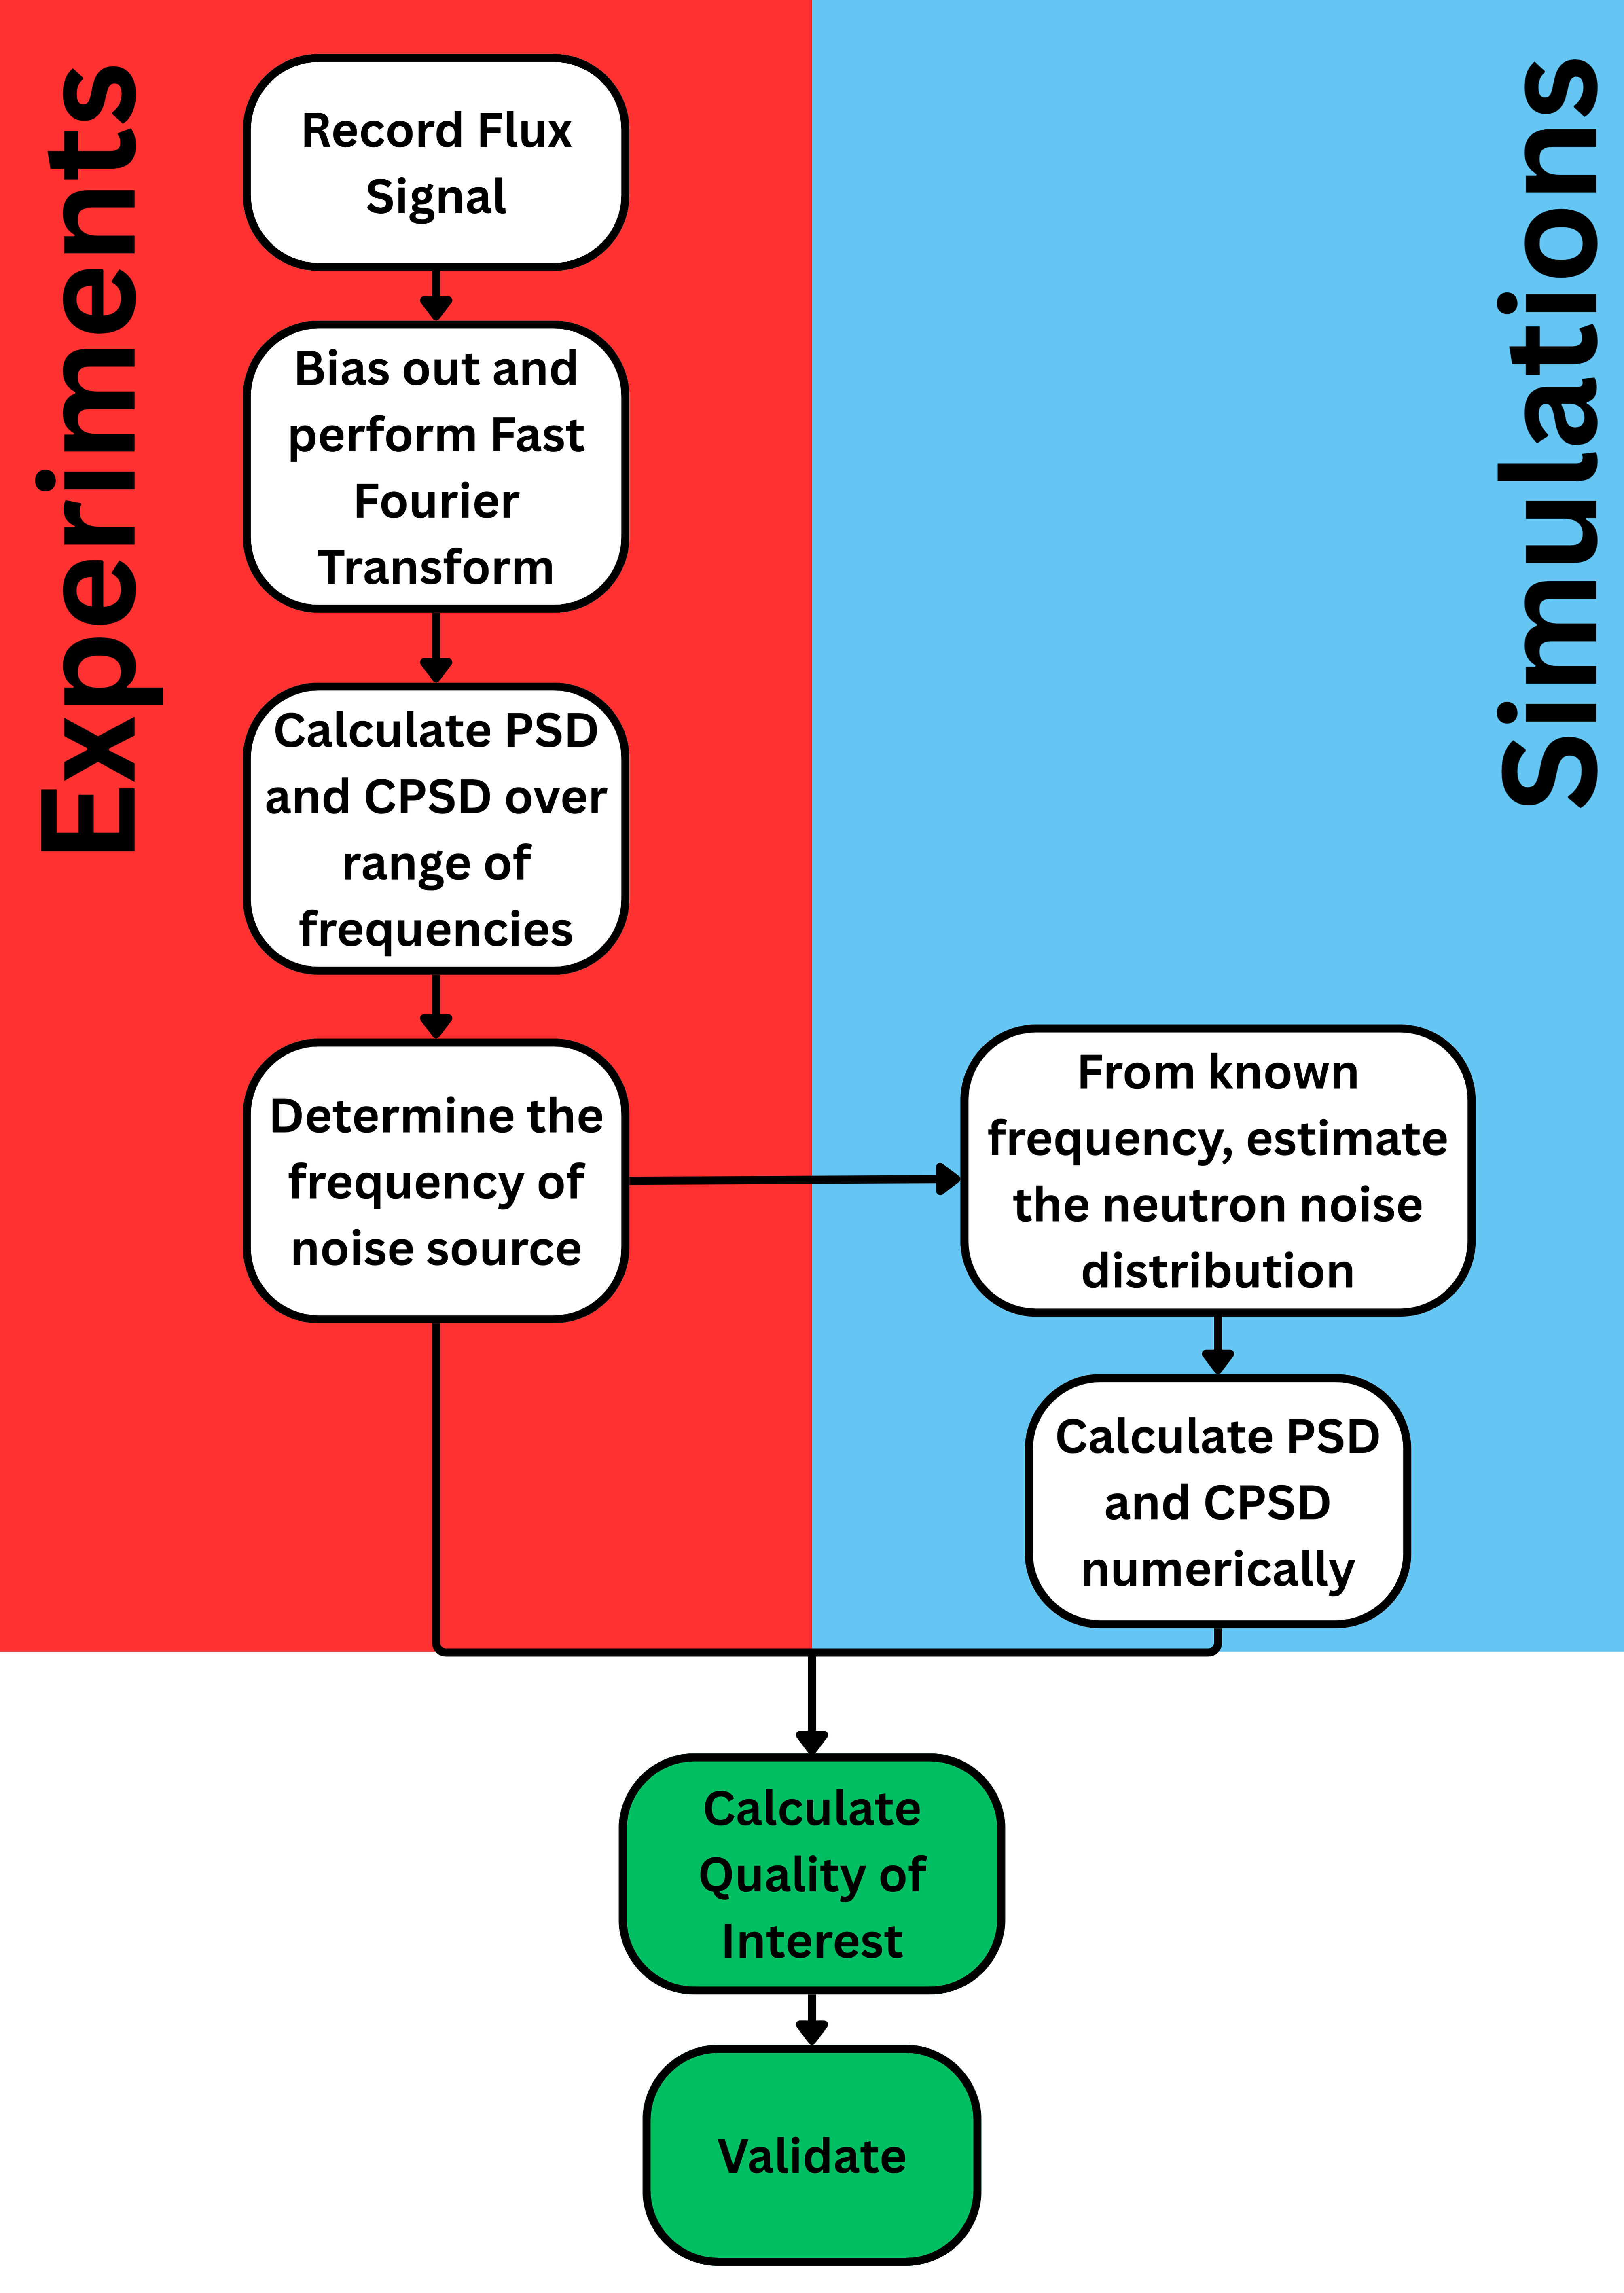
\includegraphics[width=0.5\textwidth]{figures/noise_workflow_exp1.png}
        \caption{General workflow of neutron noise experiment and simulation}
        \label{fig:flow_diagram}
\end{figure}

Assuming $\delta \phi_g (\textbf{r},\omega)$ is known from the computational method, the PSD can be determined using Welch method as follow \cite{mylonakisCORESIMSimulations2021}:

\begin{equation}
        \text{CPSD}_{xy} = \biggl(\frac{\delta \phi_{g}(\textbf{r}, \omega)}{\phi_{g}(\textbf{r})} \biggr)_x^* \cdot \biggl(\frac{\delta \phi_{g}(\textbf{r}, \omega)}{\phi_{g}(\textbf{r})} \biggr)_y
        \label{eq:CPSD_comp}
\end{equation}

To further understand the physical meaning of neutron noise, we can utilize point kinetic approximations to extract the integral parameters that characterize the reactor. To do this, we start by factorizing the time-dependent forward flux into its amplitude and shape function, such that,
\begin{equation}
        \phi (\textbf{r}, E, t) = P(t) \psi (\textbf{r}, E, t)
\end{equation}
with the following normalization condition,
\begin{equation}\label{eq:normalization}
        \frac{\partial}{\partial t} \int_{\textbf{E}} \int_{\textbf{r}} \biggl( \frac{1}{v} \phi^{\dagger}(\textbf{r}, E) \psi (\textbf{r}, E, t) \biggr) d\textbf{r} dE = 0
\end{equation}
In this case, $\phi^{\dagger}(\textbf{r}, E)$ is the solution of the adjoint equation. The normalization in Eq. \ref{eq:normalization} comes from the constraint of the variation of the flux shape in point-kinetic approximations. By having this constraint, the time dependence of the flux will largely be carried away by the amplitude function \cite{ottIntroductoryNuclearReactor1985}. Then, we split all the time-dependent components into the main values and the perturbations. Here, we define the initial condition (mean value) of the forward flux as follows,
\begin{equation}
        \phi_0(\textbf{r}, E) = P_0 \psi_0 (\textbf{r}, E)
\end{equation}
Therefore, we can write the neutron noise as follows (neglecting second-order terms),
\begin{equation}
        \begin{aligned}
                \delta \phi(\textbf{r}, E, t) &= \phi (\textbf{r}, E, t) - \phi_0(\textbf{r}, E)\\
                &= (P(t)\psi(\textbf{r}, E, t)) - \phi_0(\textbf{r}, E)\\
                &= \biggl( P_0 + \delta P(t) \biggr) \biggl( \psi_0(\textbf{r}, E)+\delta \psi(\textbf{r}, E, t) \biggr) - \phi_0(\textbf{r}, E) \\
                &= \biggl( P_0 \psi_0(\textbf{r}, E) \biggr) + \biggl(  \delta P(t) \psi_0(\textbf{r}, E)\biggr)+ \biggl(P_0 \delta \psi(\textbf{r}, E, t) \biggr) + \biggl( \delta P(t) + \delta \psi(\textbf{r}, E, t) \biggr) - \phi_0(\textbf{r}, E) \\
                &= \biggl(  \delta P(t) \psi_0(\textbf{r}, E)\biggr)+ \biggl(P_0 \delta \psi(\textbf{r}, E, t) \biggr)\\
                &= \delta P(t) \frac{\phi_0(\textbf{r}, E)}{P_0} + P_0 \delta \psi(\textbf{r}, E, t)
        \end{aligned}
        \label{eq:noise_component_time}
\end{equation}
Applying Fourier transforms to Eq. \ref{eq:noise_component_time} yields the following.
\begin{equation}\label{eq:noise_component_freq}
        \delta \phi(\textbf{r}, E, \omega) = \phi_0(\textbf{r}, E) \frac{ \delta P(\omega)}{P_0} + P_0 \delta \psi(\textbf{r}, E, \omega)
\end{equation}

Eq. \ref{eq:noise_component_freq} shows that the neutron noise can be split into two components. The first term on the right-hand side is the point-kinetic component, and the second is the spatial component of neutron noise. The point-kinetic component is driven by the reactivity effect of the perturbation, and the spatial component is driven by the nonuniform (in space) character of the perturbation \cite{pazsitNoiseTechniquesNuclear2010}.

The magnitude of power perturbation $\frac{\delta P(\omega)}{P_0}$ can be determined as follows. We can multiply Eq \ref{eq:noise_component_freq} by $\phi^{\dagger}(\textbf{r})/v$ and integrate over all the spatial and energy domains, which leads to the following.
\begin{equation}
        \int_{\textbf{E}} \int_{\textbf{r}} \frac{1}{v} \phi^{\dagger}(\textbf{r}, E) \delta \phi(\textbf{r}, E, \omega) d\textbf{r} dE = \frac{ \delta P(\omega)}{P_0} \int_{\textbf{E}} \int_{\textbf{r}} \frac{1}{v} \phi^{\dagger}(\textbf{r}, E) \phi_0(\textbf{r}, E) d\textbf{r} dE + P_0 \int_{\textbf{E}} \int_{\textbf{r}} \frac{1}{v} \phi^{\dagger}(\textbf{r}, E) \delta \psi(\textbf{r}, E, \omega) d\textbf{r} dE
        \label{eq:pk_long}
\end{equation}

Recall from Eq. \ref{eq:normalization}, we can split the shape function as follows:
\begin{equation}\label{eq:normalization_split}
\begin{aligned}
        \frac{\partial}{\partial t} \int_{\textbf{E}} \int_{\textbf{r}} \biggl( \frac{1}{v} \phi^{\dagger}(\textbf{r}, E) (\psi_0 (\textbf{r}, E) + \delta \psi (\textbf{r}, E, t) \biggr) d\textbf{r} dE &= 0 \\
        \frac{\partial}{\partial t} \int_{\textbf{E}} \int_{\textbf{r}} \biggl( \frac{1}{v} \phi^{\dagger}(\textbf{r}, E) \psi_0 (\textbf{r}, E) \biggr) d\textbf{r} dE + \frac{\partial}{\partial t} \int_{\textbf{E}} \int_{\textbf{r}} \biggl( \frac{1}{v} \phi^{\dagger}(\textbf{r}, E) \delta \psi (\textbf{r}, E, t) \biggr) d\textbf{r} dE &= 0 \\
        \frac{\partial}{\partial t} \int_{\textbf{E}} \int_{\textbf{r}} \biggl( \frac{1}{v} \phi^{\dagger}(\textbf{r}, E) \delta \psi (\textbf{r}, E, t) \biggr) d\textbf{r} dE &= 0 \\
\end{aligned}
\end{equation}

This means that Eq. \ref{eq:pk_long} can be simplified as follows:
\begin{equation}
        \frac{ \delta P(\omega)}{P_0} = \frac{\int_{\textbf{E}} \int_{\textbf{r}} \frac{1}{v} \phi^{\dagger}(\textbf{r}) \delta \phi(\textbf{r}, \omega) d\textbf{r} dE}{\int_{\textbf{E}} \int_{\textbf{r}} \frac{1}{v} \phi^{\dagger}(\textbf{r}) \phi_0(\textbf{r}) d\textbf{r} dE}
\end{equation}

Continuing with the derivation of the point kinetics component, we start from the time-dependent neutron diffusion equation, multiply both sides with adjoint flux as a weighting function, and integrate over the spatial domain, yielding the following:
\begin{equation}
    \begin{aligned}
        \frac{dP_0}{dt} + \frac{d(\delta P(t))}{dt} &= \frac{\rho_0}{\Lambda} (P_0 + \delta P(t)) + \frac{\delta \rho(t)}{\Lambda} (P_0 + \delta P(t)) - \frac{\beta}{\Lambda} (P_0 + \delta P(t)) + \lambda (C_0 + \delta C(t))\\
        \frac{dC_0}{dt} + \frac{d(\delta C(t))}{dt} &= \frac{\beta}{\Lambda} (P_0 + \delta P(t)) - \lambda (C_0 + \delta C(t))\\
    \end{aligned}
\end{equation}

By neglecting second-order terms and eliminating the time-independent component, we can simplify the equation into:
\begin{equation}
    \begin{aligned}\label{eq:simple_PRKE}
        \frac{d(\delta P(t))}{dt} &= \frac{\delta \rho(t)}{\Lambda} P_0 - \frac{\beta}{\Lambda} \delta P(t) + \lambda \delta C(t)\\
        \frac{d(\delta C(t))}{dt} &= \frac{\beta}{\Lambda} \delta P(t) - \lambda \delta C(t)\\
    \end{aligned}
\end{equation}
Applying the Fourier Transform to Eq. \ref{eq:simple_PRKE} yields to:
\begin{equation}
    \begin{aligned}\label{eq:simple_PRKE_omega}
        i \omega \delta P(\omega) &= \frac{P_0}{\Lambda} \delta \rho(\omega) - \frac{\beta}{\Lambda} \delta P(\omega) + \lambda \delta C(\omega)\\
        i \omega \delta C(\omega) &= \frac{\beta}{\Lambda} \delta P(\omega) - \lambda \delta C(\omega)\\
    \end{aligned}
\end{equation}
where $\omega = 2 \pi f$. Simplifying the precursor equation of Eq. \ref{eq:simple_PRKE_omega}, yields:
\begin{equation}
    \begin{aligned}\label{eq:simple_PRKE_precursor}
        \delta C(\omega) &= \frac{\beta}{\Lambda (i \omega + \lambda)} \delta P(\omega)\\
    \end{aligned}
\end{equation}
Then, substituting Eq. \ref{eq:simple_PRKE_precursor} to the power equation of Eq. \ref{eq:simple_PRKE_omega}, yields to:
\begin{equation}
    \begin{aligned}\label{eq:simple_power_omega}
        i \omega \delta P(\omega) &= \frac{P_0}{\Lambda} \delta \rho(\omega) - \frac{\beta}{\Lambda} \delta P(\omega) + \frac{\lambda \beta}{\Lambda (i \omega + \lambda)} \delta P(\omega)\\
        \frac{P_0}{\Lambda} \delta \rho(\omega) &= \biggl( i \omega +  \frac{\beta}{\Lambda} - \frac{\lambda \beta}{\Lambda (i \omega + \lambda)} \biggr) \delta P(\omega) \\
        \delta P(\omega) &= \delta \rho(\omega)P_0 \frac{1}{\Lambda \biggl( i \omega +  \frac{\beta}{\Lambda} - \frac{\lambda \beta}{\Lambda (i \omega + \lambda)} \biggr)} \\
        \delta P(\omega) &= \delta \rho(\omega)P_0 G(\omega)\\
    \end{aligned}
\end{equation}
Since we derive Eq. \ref{eq:simple_power_omega} from Eq. \ref{eq:freq_4}, we can explicitly define $\delta \rho(\omega)$ as follows,
\begin{equation}
        \delta \rho(\omega) = \frac{\int_{\textbf{E}} \int_{\textbf{r}} \phi^{\dagger}(\textbf{r}, E) \textbf{S}(\textbf{r}, E, \omega) d\textbf{r} dE}{\int_{\textbf{E}} \int_{\textbf{r}} \phi^{\dagger}(\textbf{r}, E) \textbf{F}(\textbf{r}, E) d\textbf{r} dE}
\end{equation}
where $\textbf{S}(\textbf{r}, \omega)$ is the noise source in the system, and $\textbf{F}(\textbf{r})$  is the fission source in the forward equation. This means that we have two ways to calculate the zero-power reactor transfer function $G(\omega)$. They are,
\begin{equation}\label{eq:ZPRTF}
        G(\omega) = \frac{1}{\Lambda \biggl( i \omega +  \frac{\beta}{\Lambda} - \frac{\lambda \beta}{\Lambda (i \omega + \lambda)} \biggr)} = \frac{\delta P (\omega) /P_0}{\delta \rho(\omega)}
\end{equation}

The zero-power reactor transfer function is one method for observing system’s behavior during a small sinusoidal perturbation. It could also be used to check whether the reactivity feedback is as expected from the design \cite{bellNuclearReactorTheory1970}. The input in ZPRTF is the reactivity perturbations ($\delta \rho (\omega)$), and the output is the power perturbations ($\frac{\delta P(\omega)}{P_0}$). It should be noted that even though the transfer function is called the zero-power reactor transfer function, Eq. \ref{eq:ZPRTF} only captures the $\delta \rho (\omega)$ response driven by the point kinetic component of the neutron noise. Therefore, it is more appropriate to call the zero-power reactor transfer function as the point kinetic zero-power reactor transfer function. An example of ZPRTF is given in Figure \ref{fig:Example2DTransferFunction}.

We can see from Figure \ref{fig:Example2DTransferFunction}, at lower frequencies, the magnitude of ZPRTF increases as the frequency decreases. This increases the point kinetic component of neutron noise, which makes the magnitude of neutron noise increases. This means that the neutron noise is dominated by the point kinetic component. At higher frequencies, the opposite happens. The magnitude of ZPRTF decreases as the frequency increases, which decreases the point kinetic component of neutron noise. In this case, the contribution of the point kinetic component to the neutron noise decreases. This means that the contribution of spatial component becomes more significant. At mid-frequencies, it is observed that there will be a plateau region in the magnitude of the transfer function in the range of $[\lambda ; \beta/\Lambda_0]$. In this region, the amplitude is nearly constant and equal to $1/\beta$. The phase of the transfer function generally will be similar to a bell curve, where the peak of the curve of the phase is close to zero \cite{demaziereDevelopmentPointkineticVerification2017}.

\begin{figure}[H]
        \centering
        \begin{subfigure}{.48\textwidth}
          \centering
          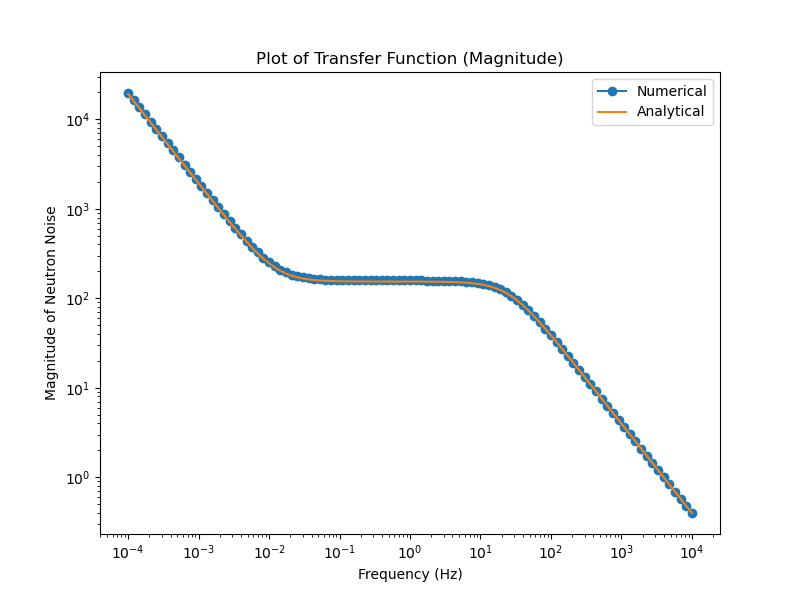
\includegraphics[width=\linewidth]{figures/OBJECTIVES3_TEST01_2DMG_BIBLIS_AVS_NOISE_Magnitude_freq.png}
        \end{subfigure}
        \hfill
        \begin{subfigure}{.48\textwidth}
          \centering
          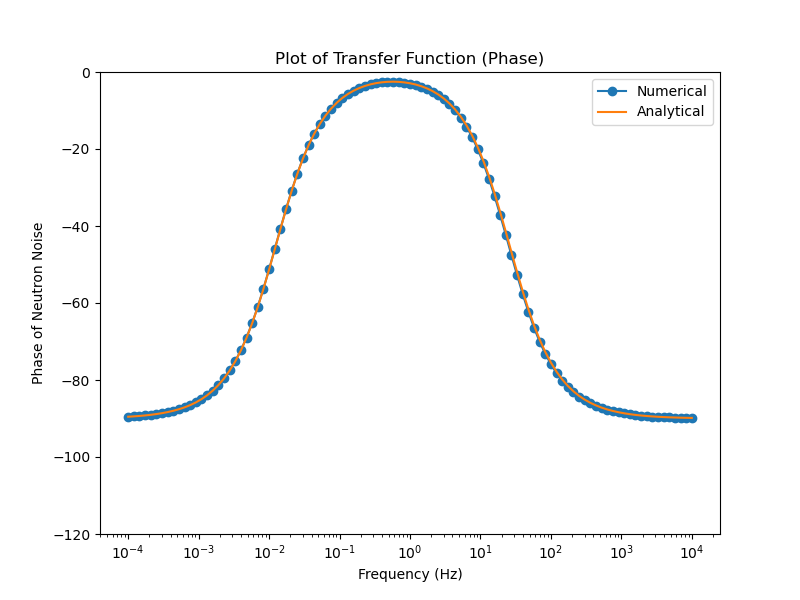
\includegraphics[width=\linewidth]{figures/OBJECTIVES3_TEST01_2DMG_BIBLIS_AVS_NOISE_Phase_freq.png}
        \end{subfigure}
        \caption{Magnitude (left) and phase delay (right) of transfer function in 2D BIBLIS Benchmark}
        \label{fig:Example2DTransferFunction}
\end{figure}

\subsection{Neutron Noise Models and Sources}

In the computational method, neutron noise sources can generally be divided into two categories. The first category is the absorber of variable strength, and the second category is called the vibrating absorber. 

\subsubsection{Absorber of Variable Strength}

Although terminology specifies absorber, these types of noise typically refer to any type of cross-sections. This includes absorption, fission, and scattering  \cite{pazsitNoiseTechniquesNuclear2010}. The absorbers of variable strength can be represented as fluctuations in the macroscopic cross-section at a given fixed location $\textbf{r}_0$ and the noise sources can be expressed as:
\begin{equation}\label{eq:AVS_FGW}
        \delta \Sigma_x (\textbf{r}, \omega) = \gamma (\omega) \delta (\textbf{r} - \textbf{r}_0)
\end{equation}
where $\gamma (\omega)$ is the noise source strength. Eq. \ref{eq:AVS_FGW} is also called the Feinberg-Galanin-Williams model \cite{pazsitNoiseTechniquesNuclear2010}. Some examples of this type of noise include the perturbations traveling with the coolant flow \cite{jonssonTwogroupTheoryNeutron2011} and perturbations due to unseated fuel assembly \cite{demaziereAnalysisMethodsDetermination2006}. In terms of modeling the noise source in a numerical tool, the absorber of variable strength can be intuitively modeled as a perturbation of cross-section in the center of computational node \cite{mylonakisCORESIMFlexible2021}. 

\subsubsection{Vibrating Absorber}

The second category is the vibrating absorber. The vibrating absorber could include vibration of the fuel assembly \cite{chionisSIMULATE3KAnalysesNeutron2017}, vibration of control rods \cite{pazsitNeutronNoiseDiagnostics1983}, or vibration of the core barrel \cite{pazsitDevelopmentsCoreBarrelMotion2016}. In the vibration absorber, the perturbation is modeled as the displacement of the vibrating assembly (or another component) from its nominal position. This is done by assuming that the neutron noise is induced by vibrating interfaces.

We can use one-dimensional perturbation as an example. Let’s assume that we have a one-dimensional system that is vibrating in one interface. We denote the equilibrium position of the vibrating interface as $x_0$. Then, we define $\Sigma_\alpha^L$ and $\Sigma_\alpha^R$ as macroscopic cross sections of the region at the left ($x<x_0$) and at the right ($x>x_0$) of the vibrating interface. We assume that the vibration in the interface is periodic with frequency $\omega_0$, and amplitude $\varepsilon$, which is smaller than the side $d$ of the region of interest in the interface perturbation. Figure \ref{fig:1Dvibration} illustrates the vibrating absorber case in 1D \cite{zoiaAnalysisNeutronNoise2021}.
\begin{figure}[H]
        \centering
        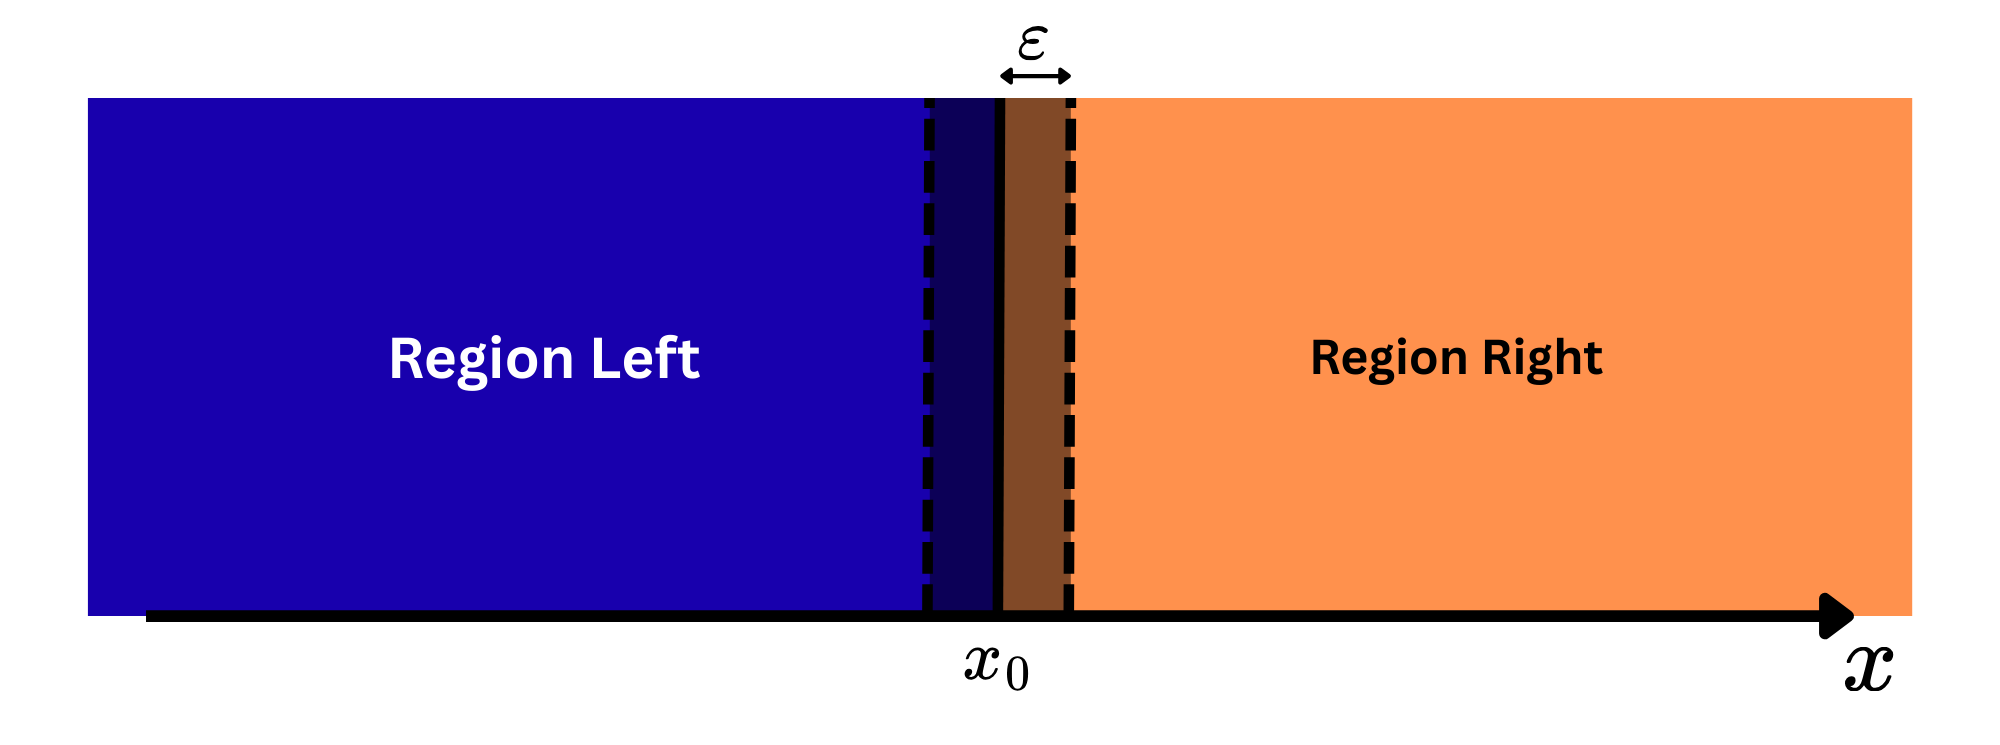
\includegraphics[width=0.5\textwidth]{figures/Region Left.png}
        \caption{Example of vibrating absorber noise source in 1D}
        \label{fig:1Dvibration}
\end{figure}

In this case, the position of the moving interface $x_i (t)$ and the perturbation $\delta\Sigma_\alpha (x, E, t)$ can be written as follows:
\begin{equation}
    x_i(t) = x_0 + \varepsilon \sin(\omega_0 t)
\end{equation}
\begin{equation}\label{eq:dABS_exact}
    \delta\Sigma_\alpha (x, E, t) = \biggl(\Sigma_\alpha^L (x, E)-\Sigma_\alpha^R (x, E)\biggr) \biggl( H(x-x_0)-H(x-x_0-\varepsilon \sin(\omega_0 t) \biggr)
\end{equation}

Where $H(x-x_0)$ is the Heaviside function. This means that the value of $\delta\Sigma_\alpha (x, E, t)$ is non-zero only at the perturbed area, which $x-\varepsilon \leq x \leq x+\varepsilon$ \cite{zoiaAnalysisNeutronNoise2021}. From Eq. \ref{eq:dABS_exact}, we can perform Fourier transformations by dividing into two different regions, $x<x_0$ and $x>x_0$. This will lead to the definition of the neutron noise source for periodic vibrating absorber. 

For $\varepsilon\ll d$, one could perform an approximation called the weak absorber approximation, also known as the $\varepsilon/d$ model \cite{pazsitInvestigationSpaceDependentNoise1977}. This model indicates that the magnitude of the perturbation is so small compared to the reactor size that it can be converted into a spatially localized cross-section perturbation. The weak absorber approximation is done by performing a Taylor series expansion to Eq. \ref{eq:dABS_exact} in powers of $\varepsilon$, which yields the following:
\begin{equation}\label{eq:dABS_taylor}
    \delta\Sigma_\alpha (x, E, t) = \biggl(\Sigma_\alpha^L (x, E)-\Sigma_\alpha^R (x, E)\biggr) \biggl( \varepsilon \sin(\omega_0 t) \delta(x-x_0)-\frac{\varepsilon^2 \sin^2(\omega_0 t)}{2} \delta'(x-x_0)+ ... \biggr)
\end{equation}
Performing Fourier transform to Eq. \ref{eq:dABS_taylor} yields the following:
\begin{equation}\label{eq:dABS_taylor_omega}
    \delta\Sigma_\alpha (x, E, \omega) = \biggl(\Sigma_\alpha^L (x, E)-\Sigma_\alpha^R (x, E)\biggr) \biggl( -i \pi \varepsilon \delta(x-x_0) \delta(\omega-\omega_0)-\frac{\pi}{4} \varepsilon^2 \delta'(x-x_0) \delta(\omega-2\omega_0)+ ... \biggr)
\end{equation}

From Eq. \ref{eq:dABS_taylor_omega}, we can see that the periodic vibration can be approximated as a series of frequencies \cite{zoiaAnalysisNeutronNoise2021}. Some literature shows that the second harmonic might be relevant in some cases \cite{luciaCorrelationNeutronNoise1973, pazsitInvestigationSpaceDependentNoise1977, pazsitLinearizationVibrationinducedNoise1984}. However, previous works in $\varepsilon/d$ approximation only consider the first order effect, which yields the following.
\begin{equation}\label{eq:dABS_taylor_omega_truncated}
    \delta\Sigma_\alpha (x, E, \omega) = \biggl(\Sigma_\alpha^L (x, E)-\Sigma_\alpha^R (x, E)\biggr) \biggl( -i \pi \varepsilon \delta(x-x_0) \delta(\omega-\omega_0) \biggr)
\end{equation}
In terms of modeling the noise source in a numerical tool, the vibrating absorbers can be modeled as a perturbation of cross-sections at the boundary of the vibrating region \cite{mylonakisCORESIMFlexible2021}.

The vibrating absorber model shown in this chapter (which will be used for the remainder of the dissertation) comes from the linearization of vibration-induced noise, which yields an idealized delta function that eventually leads to Eq. \ref{eq:dABS_taylor_omega_truncated}.  When this absorber model is applied as the noise source in Eq. \ref{eq:freq_4}, it will provide accurate estimates for the neutron noise when $\varepsilon/d \ll 1$. Linearization of the vibrating absorber model means that the system only responds at frequency $\omega_0$. This brings up the issue of an effect called the “double frequency” effect, which means that a system subject to a periodic vibration at frequency $\omega_0$ could have a secondary peak at frequency $2\omega_0$. This double-frequency effect has been demonstrated in some experiments \cite{luciaCorrelationNeutronNoise1973}. By linearizing the vibration noise source, the secondary peak is no longer observable.  

\section{Existing Computational Tools of Neutron Noise Analysis}
\label{sec:noise_tools}

\subsection{Solving Neutron Noise Problems using Deterministic Methods}

Deterministic transport methods have been developed to solve the neutron noise equation. It should be noted that knowledge of the forward neutron flux distribution and k-criticality is necessary to perform neutron noise simulations, as these parameters become the input to the neutron noise simulation. The tools developed varied in terms of spatial discretization, energy discretization, angular discretization, and the domain of interest to solve the neutron noise equation. The following list shows the development of neutron noise simulation tools using deterministic methods. This list is sorted based on the time at which the literature has been published.
\begin{itemize}
    \item Demazi\`ere developed a 2-group, 2-dimensional (cartesian) neutron noise simulator in frequency domain. The simulator used finite difference for spatial discretization. The simulator calculated the neutron noise and the corresponding adjoint functions \cite{demaziereDevelopment2D2group2004}.
    \item Malmir et al. developed a 2-group, 2-dimensional neutron noise simulator for hexagonal geometries. The neutron noise simulator is in frequency domain. The box-scheme finite difference method for hexagonal mesh was used for spatial discretization. The spatial discretization is performed by splitting each hexagon into seven hexagonal mesh boxes. The simulation of neutron noise in VVER-1000 has been applied to this simulator \cite{malmirDevelopment2D2group2010}.
    \item Larsson et al. developed a 2-group, 2-dimensional (cartesian) neutron noise simulator in frequency domain. The simulator used analytical nodal method (ANM) for spatial discretization. ANM is used to solve for both forward flux and neutron noise calculations \cite{larssonNeutronNoiseCalculations2011}.
    \item Demazi\`ere developed a multi-purpose neutronic tool called CORE SIM. CORE SIM is a 2-group, 3-dimensional (cartesian) simulator. It uses finite difference for spatial discretization. It has the capability to solve forward, adjoint, and neutron noise equations. The neutron noise equation is solved in frequency domain \cite{demaziereCORESIMMultipurpose2011}.
    \item Tran et al. developed a tool for neutron noise equation in hexagonal geometries. The tool is a multigroup, 2-dimensional (hexagonal) simulator. It uses finite difference for spatial discretization. It has been compared with analytical solutions based on 2-dimensional 2-group homogeneous systems \cite{tranNeutronNoiseCalculations2013}.
    \item Rouchon et al. developed a neutron noise tool in the APOLLO3. APOLLO3 is a 3-dimensional (cartesian) multigroup diffusion tool. It uses Nodal Expansion Method (NEM) for spatial discretization \cite{schneiderAPOLLO3CEADeterministic2016}. The neutron noise simulation is performed using frequency domain. In APOLLO3, the neutron noise simulation is performed by changing the production operator into complex number, and adding an iteration loop between the real and imaginary parts of the neutron noise equation \cite{rouchonNew3DMultigroup2017}.
    \item Rohde et al. simulated neutron noise in time domain using DYN3D. DYN3D is a three-dimensional best-estimate tool for simulating steady states and transients of LWRs \cite{rohdeReactorDynamicsCode2016}. The neutron noise simulation is performed for a generic KONVOI reactor core. The neutron noise is induced by coolant inlet temperature variations, channel-wise mass-flow rate variation, and variation in the local moderator density in a part of the core \cite{rohdeNeutronNoiseObservations2018}.
    \item Chionis et al. developed a neutron noise tool in the SIMULATE-3K code (S3K). S3K is 2-group nodal code for transient analysis. For neutron noise simulation, the code uses time domain analysis. The code is applied to analyze fuel assembly vibration in the Swiss PWR \cite{chionisSIMULATE3KAnalysesNeutron2017}. The same tool is also used to simulate fuel assembly vibrations in KWU pre-KONVOI reactors \cite{vermaModellingAnalysisFuel2021}.
    \item Bahrami et al. developed a neutron noise tool based on SN method. The neutron noise equation is solved using Green’s function in frequency domain. The tool has been applied to several benchmarks problems and compared to diffusion-based neutron noise tool. The results show that the difference between SN-based and diffusion-based methods are noticeable in the media with less than 100 mean free path thickness as well as source locations near the edge. In these cases, more comprehensive tests are necessary \cite{bahramiSNTransportMethod2018}.
    \item Vidal-Ferrandiz et al. developed FEMFFUSION. FEMFFUSSION is a 3-dimensional, 2-group neutron diffusion simulator that uses a finite element method to solve the neutron diffusion equation. FEMFFUSION solves the neutron noise equation in the time domain \cite{vidal-ferrandizNeutronicSimulationFuel2020}.
    \item Mylonakis et al. developed CORE SIM+, which is the extension of CORE SIM. CORE SIM+ has the capability to solve non-unform meshes. It also has the capability to generate Green’s functions for solving neutron noise equation \cite{mylonakisCORESIMFlexible2021}.
    \item Gong et al. developed a prototype code called CORCA-NOISE. CORCA-NOISE is a multigroup neutron noise tool based on the simplified P3 method for the angular discretization. It is part of the industry SP3 tool CORCA-PIN, which is developed by the Nuclear Power Institute of China (NPIC). It uses finite element method for spatial discretization. This tool has been compared to CORE SIM for two benchmark studies \cite{gongNeutronNoiseCalculation2021}.
    \item Yi et al. developed a neutron noise tool called the NOISE-SN. NOISE-SN is a multigroup, 3-dimensional (cartesian) neutron noise tool based on the SN method for angular discretization. It uses diamond finite difference for the spatial discretization. The tool is compared with CORE SIM+ using C4V and C5G7 benchmarks \cite{yiSimulationNeutronNoise2021}.
\end{itemize}

\subsection{Solving Neutron Noise Problems using Monte Carlo Methods}

Monte Carlo method has been used to solve neutron noise equations. Several methods are developed to solve the neutron noise equation from transport theory. Some others developed Monte Carlo method to solve Green’s function using Monte Carlo. Compared to a conventional fixed source transport equation, the neutron noise equation (see Eq. \ref{eq:freq_4}) has three main differences. First, the solution of neutron noise equation, $\delta \phi(\textbf{r},\Omega, E, \omega)$, is a complex value. Second, the production term is multiplied by a complex-value factor $\biggl( \chi^p_g (1-\beta_{\text{eff}}) + \chi^d_g \frac{\lambda \beta_{\text{eff}}}{i \omega + \lambda} \biggr)$. Third, the addition of $\frac{i \omega}{v} \delta \phi(\textbf{r},\Omega, E, \omega)$ in the equation. The following list shows the use of Monte Carlo method to solve neutron noise equation.
\begin{itemize}
    \item Yamamoto developed a method to solve neutron noise equations using Monte Carlo method \cite{yamamotoMonteCarloMethod2013}. The method is developed based on the neutron leakage-corrected calculation using complex-weighted Monte Carlo method \cite{yamamotoMonteCarloMethod2012}. The strategy of solving neutron noise equation using Monte Carlo method is divided into three parts. First, the method introduces complex-valued weights for each simulated neutron noise particle. These weights can have positive or negative signs. Second, as the particle transported, the method performed weight cancellation of positive and negative weights. The weight cancellation is necessary to avoid the production of too many neutron noise particles at low and very high frequencies. Third, the method includes the additional term $\frac{i \omega}{v} \delta \phi(\textbf{r},\Omega, E, \omega)$ during the random walk processes of the particles with complex-valued weights. For verification purposes, this method has been verified with analytical solutions and comparison with diffusion theory. The results show that the diffusion theory yields less accurate results compared to Monte Carlo method for higher frequency noise sources \cite{yamamotoMonteCarloMethod2013}.
    \item Rouchon et al. developed a new Monte Carlo-based method to solve neutron noise equation \cite{rouchonNewMonteCarlo2017}. Similar to \cite{yamamotoMonteCarloMethod2013}, the method is based on transporting complex-valued neutron noise particles. However, the method introduces a new term to the neutron noise equation $\frac{(\eta - i)}{\eta} \eta \frac{\omega}{v} \delta \phi (\textbf{r}, \omega)$, where $\eta$ is a real constant with the same sign as $\omega$. By having this modification, the method can use conventional algorithms for fixed source problems for all frequencies. This method also does not need any weight cancellation techniques for low and very high frequencies. This method has been compared to \cite{yamamotoMonteCarloMethod2013} and shows that the method has better Figure of Merit (FoM) compared to \cite{yamamotoMonteCarloMethod2013}.
    \item Demaziere et al. developed a Monte Carlo-based method that leverages Green’s function for solving neutron noise equation. Starting from neutron noise equation in frequency domain, the authors split the equation in coupled balance equation, representing the real part and imaginary part of neutron noise. To solve these coupled equations using Monte Carlo code, the reaction rates in each equation need to be positive. Demaziere et al. rewrote the coupled equation such that the reaction rates are positive. Then, the solution of neutron noise can be obtained using Green’s functions that are generated using Monte Carlo simulations \cite{demaziereMonteCarlobasedDynamic29}.
\end{itemize}

\section{Conclusion}

This chapter provides a general overview of neutron noise. Neutron noise analysis has been implemented in nuclear reactors, especially for anomaly detections. Computational methods of neutron noise have been derived and reviewed in this chapter. This chapter also derived the point kinetics approximation of neutron noise equation to obtain several parameters (e.g. power perturbations, reactivity perturbations, and zero-power reactor transfer functions). This chapter reviews different models of neutron noise sources and its implementation to computational method. This chapter also provides several tools that have been developed to solve neutron noise equation, both using deterministic and Monte Carlo methods.

%=======================================================================

\chapter{Computational Tool for Neutron Noise Simulations}
\label{ch:simulations}

The previous chapter explained that the history of the neutron noise method began as part of the core diagnostics methods performed in a nuclear reactor. Seeing the success of the technique, computational methods to solve the neutron noise have also been developed \cite{demaziereCORTEXProjectImproving2020}. To perform reactor diagnostics using neutron noise analysis computationally, the tool must have the capability to perform neutron noise calculations, forward flux calculations, and generate the Green’s function matrix. The forward flux is part of the source term in the neutron noise equation, which will be shown in the next section. The Green’s function is used as part of the neutron noise unfolding method. The adjoint flux is used to determine the characteristics of neutron noise (e.g. neutron noise components and ZPRTF) as shown in Section \ref{sec:noise_derivation}. Numerous efforts have been made to computationally solve the neutron noise equation. Several examples of tools have been mentioned in the previous chapter.

Forward, adjoint, neutron noise, and Green's function simulator is not a unique problem to solve. There has been many tool developed for these purposes. Tools such as CORE SIM+ \cite{mylonakisCORESIMFlexible2021} can perform forward, adjoint, and noise calculations, as well as generate the Green’s function matrix. Another tool, such as FEMFFUSION \cite{vidal-ferrandizFEMFFUSIONFiniteElement2023}, can perform forward, adjoint, and noise calculations for rectangular and triangular mesh using a finite element method. Other examples of tools have been mentioned in Section \ref{sec:noise_tools}. In this dissertation, a numerical tool for neutron noise analysis is developed to ensure a consistency between the solutions of forward flux, adjoint flux, neutron noise, and the Green's function. By developing a unified numerical tool, all four calculations share the same numerical framework, discretization, and data structures, eliminating discrepancies that can arise when mixing external tools with different discretization strategies. The tool is based on on a multigroup diffusion equation and a finite volume method for spatial discretization. The tool is available in \href{https://github.com/harunardi/FANGS-UNFOLD}{GitHub}\footnote{https://github.com/harunardi/FANGS-UNFOLD} for future references.

The structure of this chapter is as follows. First, we review the neutron noise equation, which was derived in the previous chapter. This includes the forward and adjoint equations, as well as the inputs and outputs for each equation. Then, we focus on the spatial discretization method using the finite volume method and how it is applied to 3D triangular geometries for each equation. We also explain the boundary conditions that can be used in the tool. Lastly, we provide some case examples for verifying the tool.

\section{The Neutron Noise Equation}
The neutron noise equation has been derived in the previous chapter. The equation is given in Eq. \ref{eq:freq_4}, which is repeated here for convenience:
\begin{equation}
        \begin{aligned}
                \frac{i \omega}{v_g} \delta \phi_g (\textbf{r}, \omega) - \nabla D_g(\textbf{r}) \nabla \delta \phi_g(\textbf{r}, \omega) + \Sigma_{t,g,0}(\textbf{r}) \delta \phi_g(\textbf{r}, \omega) - \sum_{g' = 1}^{G} \biggl(\Sigma_{s0,g',g,0}(\textbf{r}) \delta \phi_{g'}(\textbf{r}, \omega) \biggr) -\\ \frac{1}{k_{\text{eff}}} \biggl( \chi^p_g (1-\beta_{\text{eff}}) + \chi^d_g \frac{\lambda \beta_{\text{eff}}}{i \omega + \lambda} \biggr)  \biggl(\sum_{g' = 1}^{G} \nu \Sigma_{f,g',0}(\textbf{r}) \delta \phi_{g'}(\textbf{r}, \omega) \biggr)= \\
                - \delta \Sigma_{t,g}(\textbf{r}, \omega) \phi_{g,0}(\textbf{r}) + \sum_{g' = 1}^{G} \biggl(\delta \Sigma_{s0,g',g}(\textbf{r}, \omega) \phi_{g',0}(\textbf{r}) \biggr)\\
                \frac{1}{k_{\text{eff}}} \biggl( \chi^p_g (1-\beta_{\text{eff}}) + \chi^d_g \frac{\lambda \beta_{\text{eff}}}{i \omega + \lambda} \biggr)  \biggl( \sum_{g' = 1}^{G} \delta \nu \Sigma_{f,g'}(\textbf{r}, \omega) \phi_{g',0}(\textbf{r}) \biggr)
        \end{aligned}
        \label{eq:freq_4_ch3}
\end{equation}
Eq. \ref{eq:freq_4_ch3} shows the multigroup neutron noise equation in the frequency domain, where $\delta \phi_g (\textbf{r}, \omega)$ is the group-wise neutron noise and $\omega$ is the angular frequency (radians per second). The unknown (output) of the equation is the neutron noise, $\delta \phi_g (\textbf{r}, \omega)$ with unit of $\frac{n}{cm^2}$, the knowns (inputs) are the macroscopic cross sections and the noise source.

In Eq. \ref{eq:freq_4_ch3}, the noise source is defined as the combination of perturbed macroscopic cross sections and the forward flux $\phi_{g,0} (\textbf{r})$. The forward flux is obtained from the steady-state multigroup neutron diffusion equation \cite{duderstadtNuclearReactorAnalysis1977}, shown in Eq. \ref{eq:forward_eq_ch3}.
\begin{equation}
        \begin{aligned}
                - \nabla D_g(\textbf{r}) \nabla \phi_{g,0}(\textbf{r}) + \Sigma_{t,g,0}(\textbf{r}) \phi_{g,0}(\textbf{r}) = \sum_{g' = 1}^{G} \biggl(\Sigma_{s0,g',g,0}(\textbf{r}) \phi_{g',0}(\textbf{r}) \biggr) \\
                + \frac{1}{k_{\text{eff}}} \biggl( \chi^p_g (1-\beta_{\text{eff}}) + \chi^d_g \beta_{\text{eff}} \biggr)  \biggl( \sum_{g' = 1}^{G} \nu \Sigma_{f,g',0}(\textbf{r}) \phi_{g',0}(\textbf{r}) \biggr)
        \end{aligned}
        \label{eq:forward_eq_ch3}
\end{equation}
In Eq. \ref{eq:forward_eq_ch3}, the knowns (input) are the macroscopic cross sections, the unknown (outputs) are the forward flux and the criticality $k_{\text{eff}}$. 

The tool also solve the multigroup adjoint equation \cite{duderstadtNuclearReactorAnalysis1977}, as it is important for calculating the neutron noise components and zero-power reactor transfer function:
\begin{equation}
        \begin{aligned}
                - \nabla D_g(\textbf{r}) \nabla \phi^{\dagger}_{g,0}(\textbf{r}) + \Sigma_{t,g,0}(\textbf{r}) \phi^{\dagger}_{g,0}(\textbf{r}) = \sum_{g' = 1}^{G} \biggl(\Sigma_{s0,g,g',0}(\textbf{r}) \phi^{\dagger}_{g',0}(\textbf{r}) \biggr) \\
                + \frac{1}{k_{\text{eff}}} \nu \Sigma_{f,g,0}(\textbf{r}) \biggl( \sum_{g' = 1}^{G} \bigl( \chi^p_{g'} (1-\beta_{\text{eff}}) + \chi^d_{g'} \beta_{\text{eff}} \bigr) \phi^{\dagger}_{g',0}(\textbf{r}) \biggr)
        \end{aligned}
        \label{eq:adjoint_eq_ch3}
\end{equation}
Here, the known (inputs) are the macroscopic cross sections, the unknown (outputs) are the adjoint flux and the criticality $k_{\text{eff}}$.

\section{The Neutron Noise tool}

\subsection{Spatial Discretization for Triangular Geometries}

In this chapter, the 3D system for triangular geometries are derived. The neutron noise tool is developed using the finite volume method as the spatial discretization method. In case of hexagonal assembly, it is divided into 6 equilateral triangles, and mesh refinement is done by subdividing each triangle into 4 equilateral triangles. The total number of triangles in the hexagon is defined as follows:
\begin{equation}
    n = 6 \times 4^{\text{level}}
\end{equation}
where “level” is the mesh refinement level, which indicates how many times the triangular meshes have been subdivided. This means that level 0 consists of 6 triangles (no subdivision), level 1 consists of 24 triangles (subdivided once), level 2 consists of 96 triangles (subdivided twice), and so on. Figure \ref{fig:2DTri discretization} shows how the indexing of the triangular grid works. The visual representation of the discretization for 3D triangular geometries is shown in Figure \ref{fig:3DTri discretization}.

\begin{figure}[H]
        \centering
        \begin{subfigure}{.48\textwidth}
          \centering
          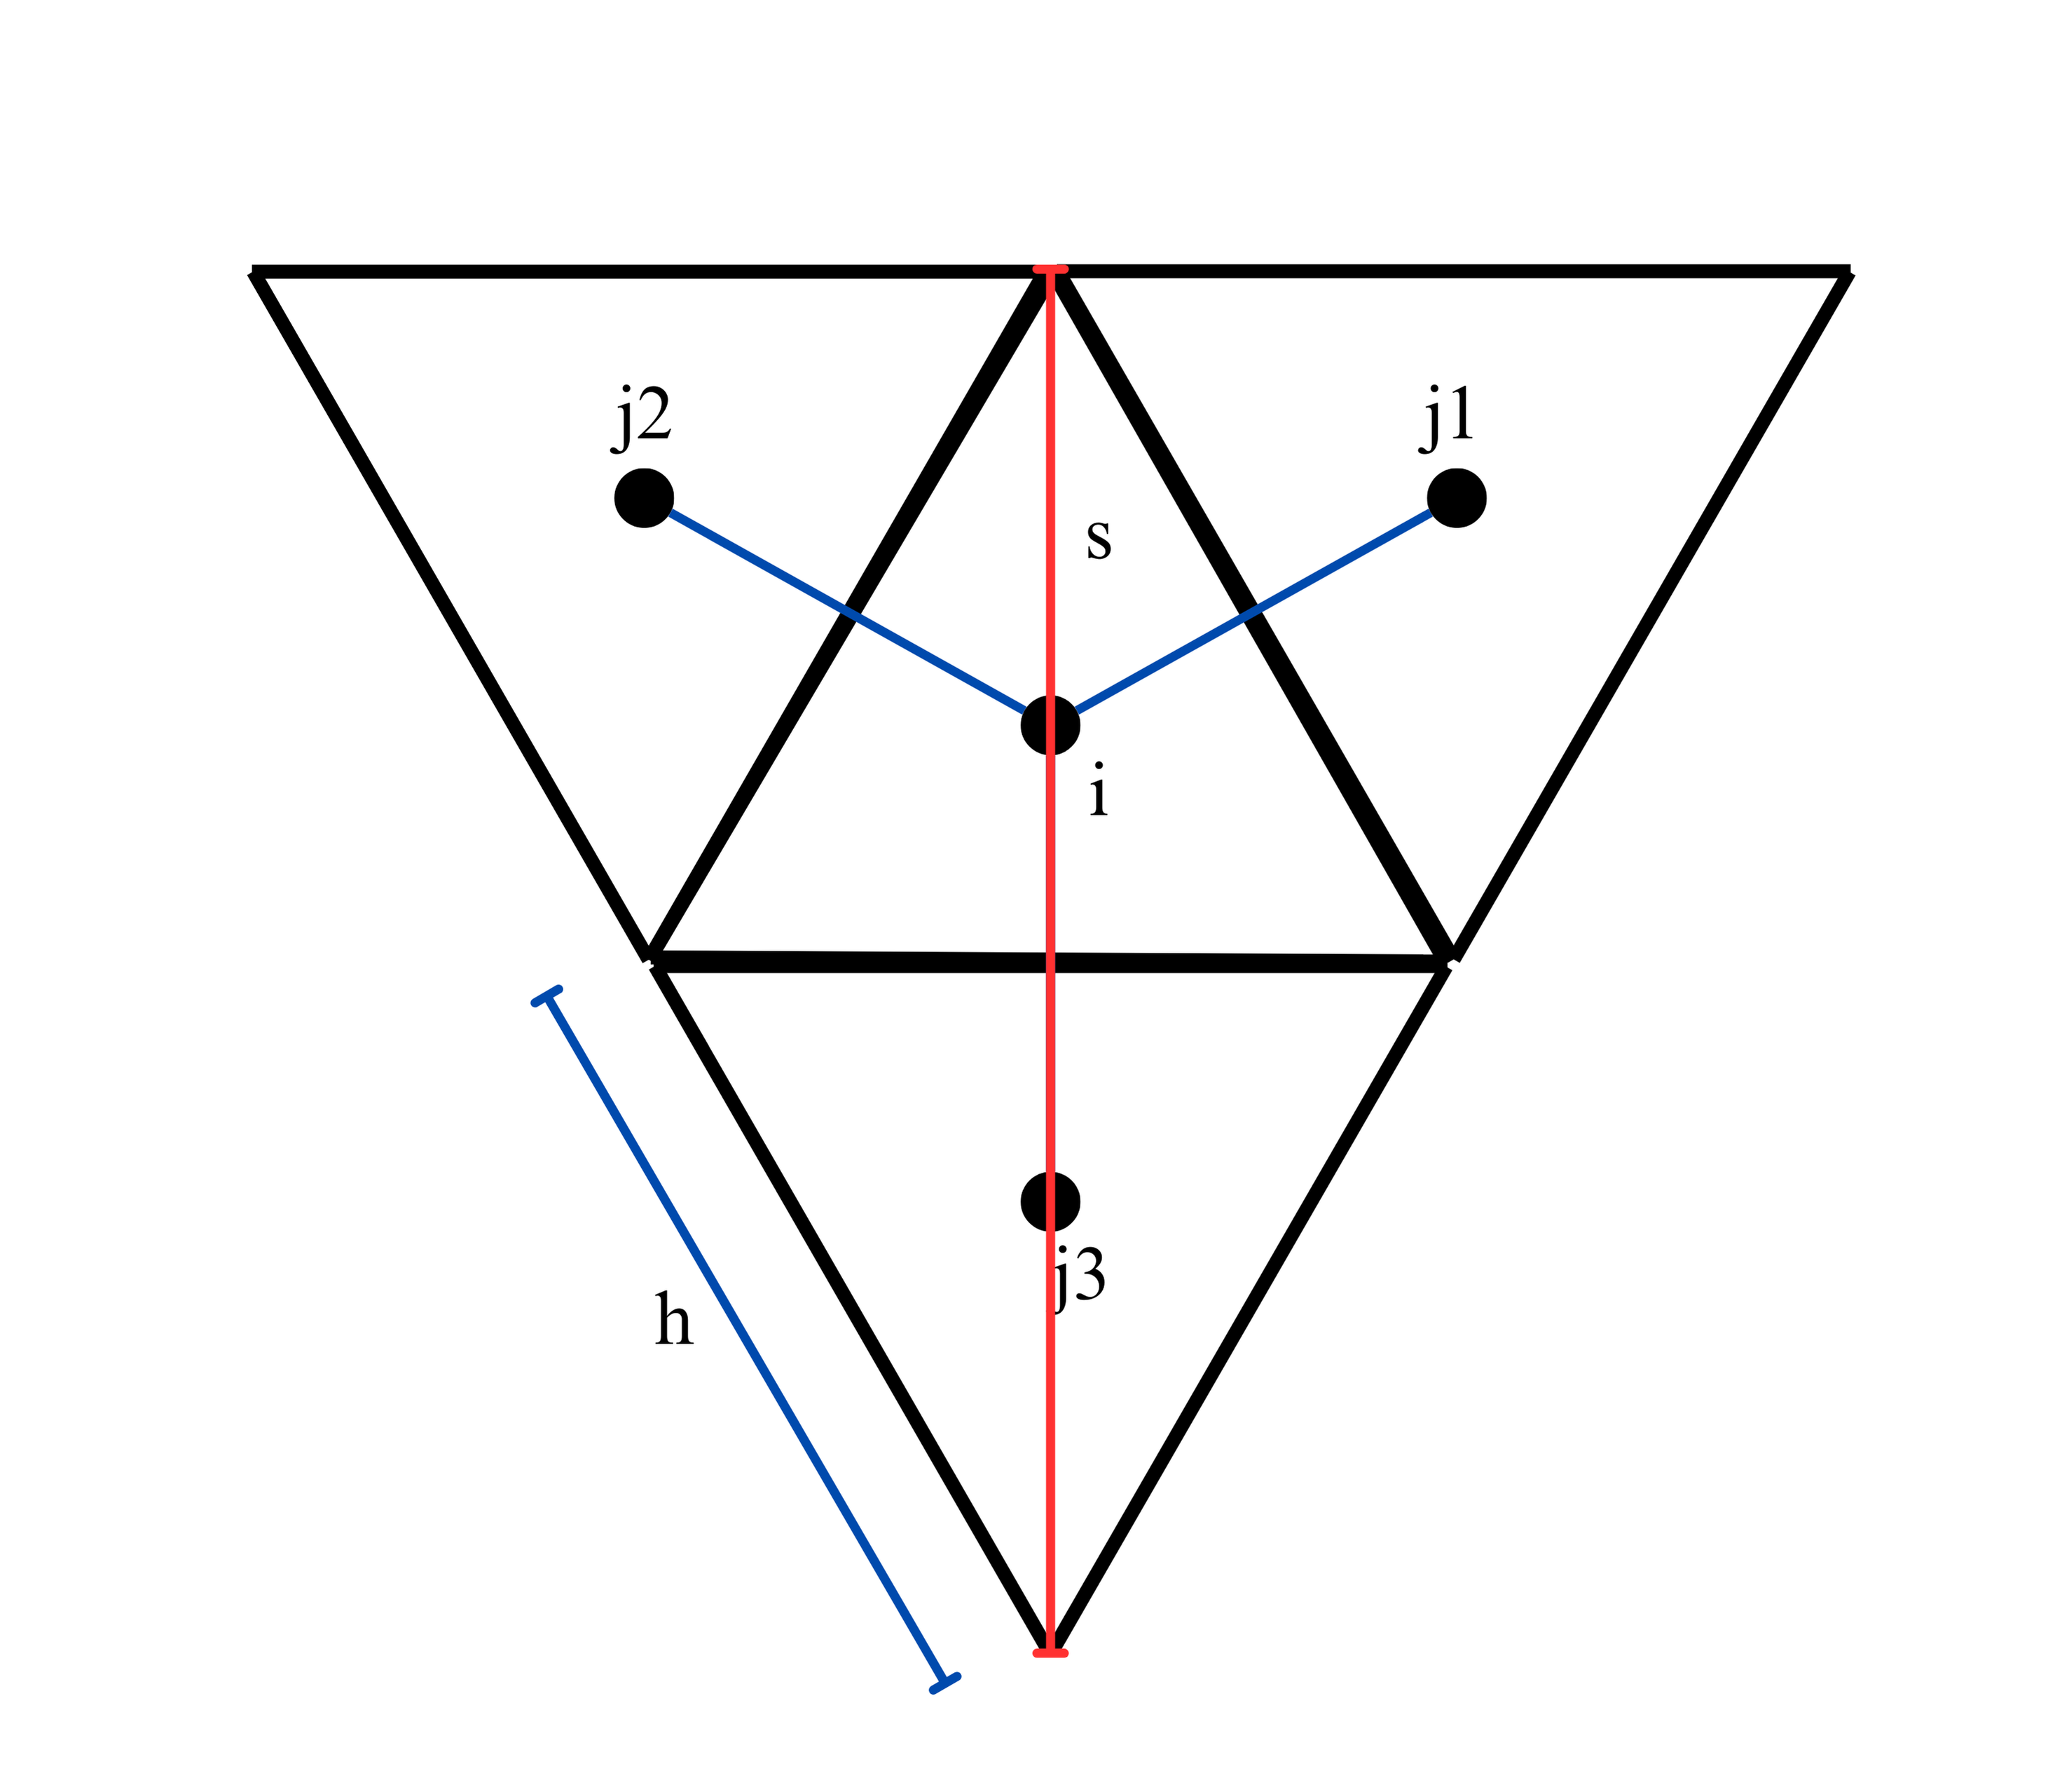
\includegraphics[width=\linewidth]{figures/disc_hexx.png}
        \end{subfigure}
        \hfill
        \begin{subfigure}{.48\textwidth}
          \centering
          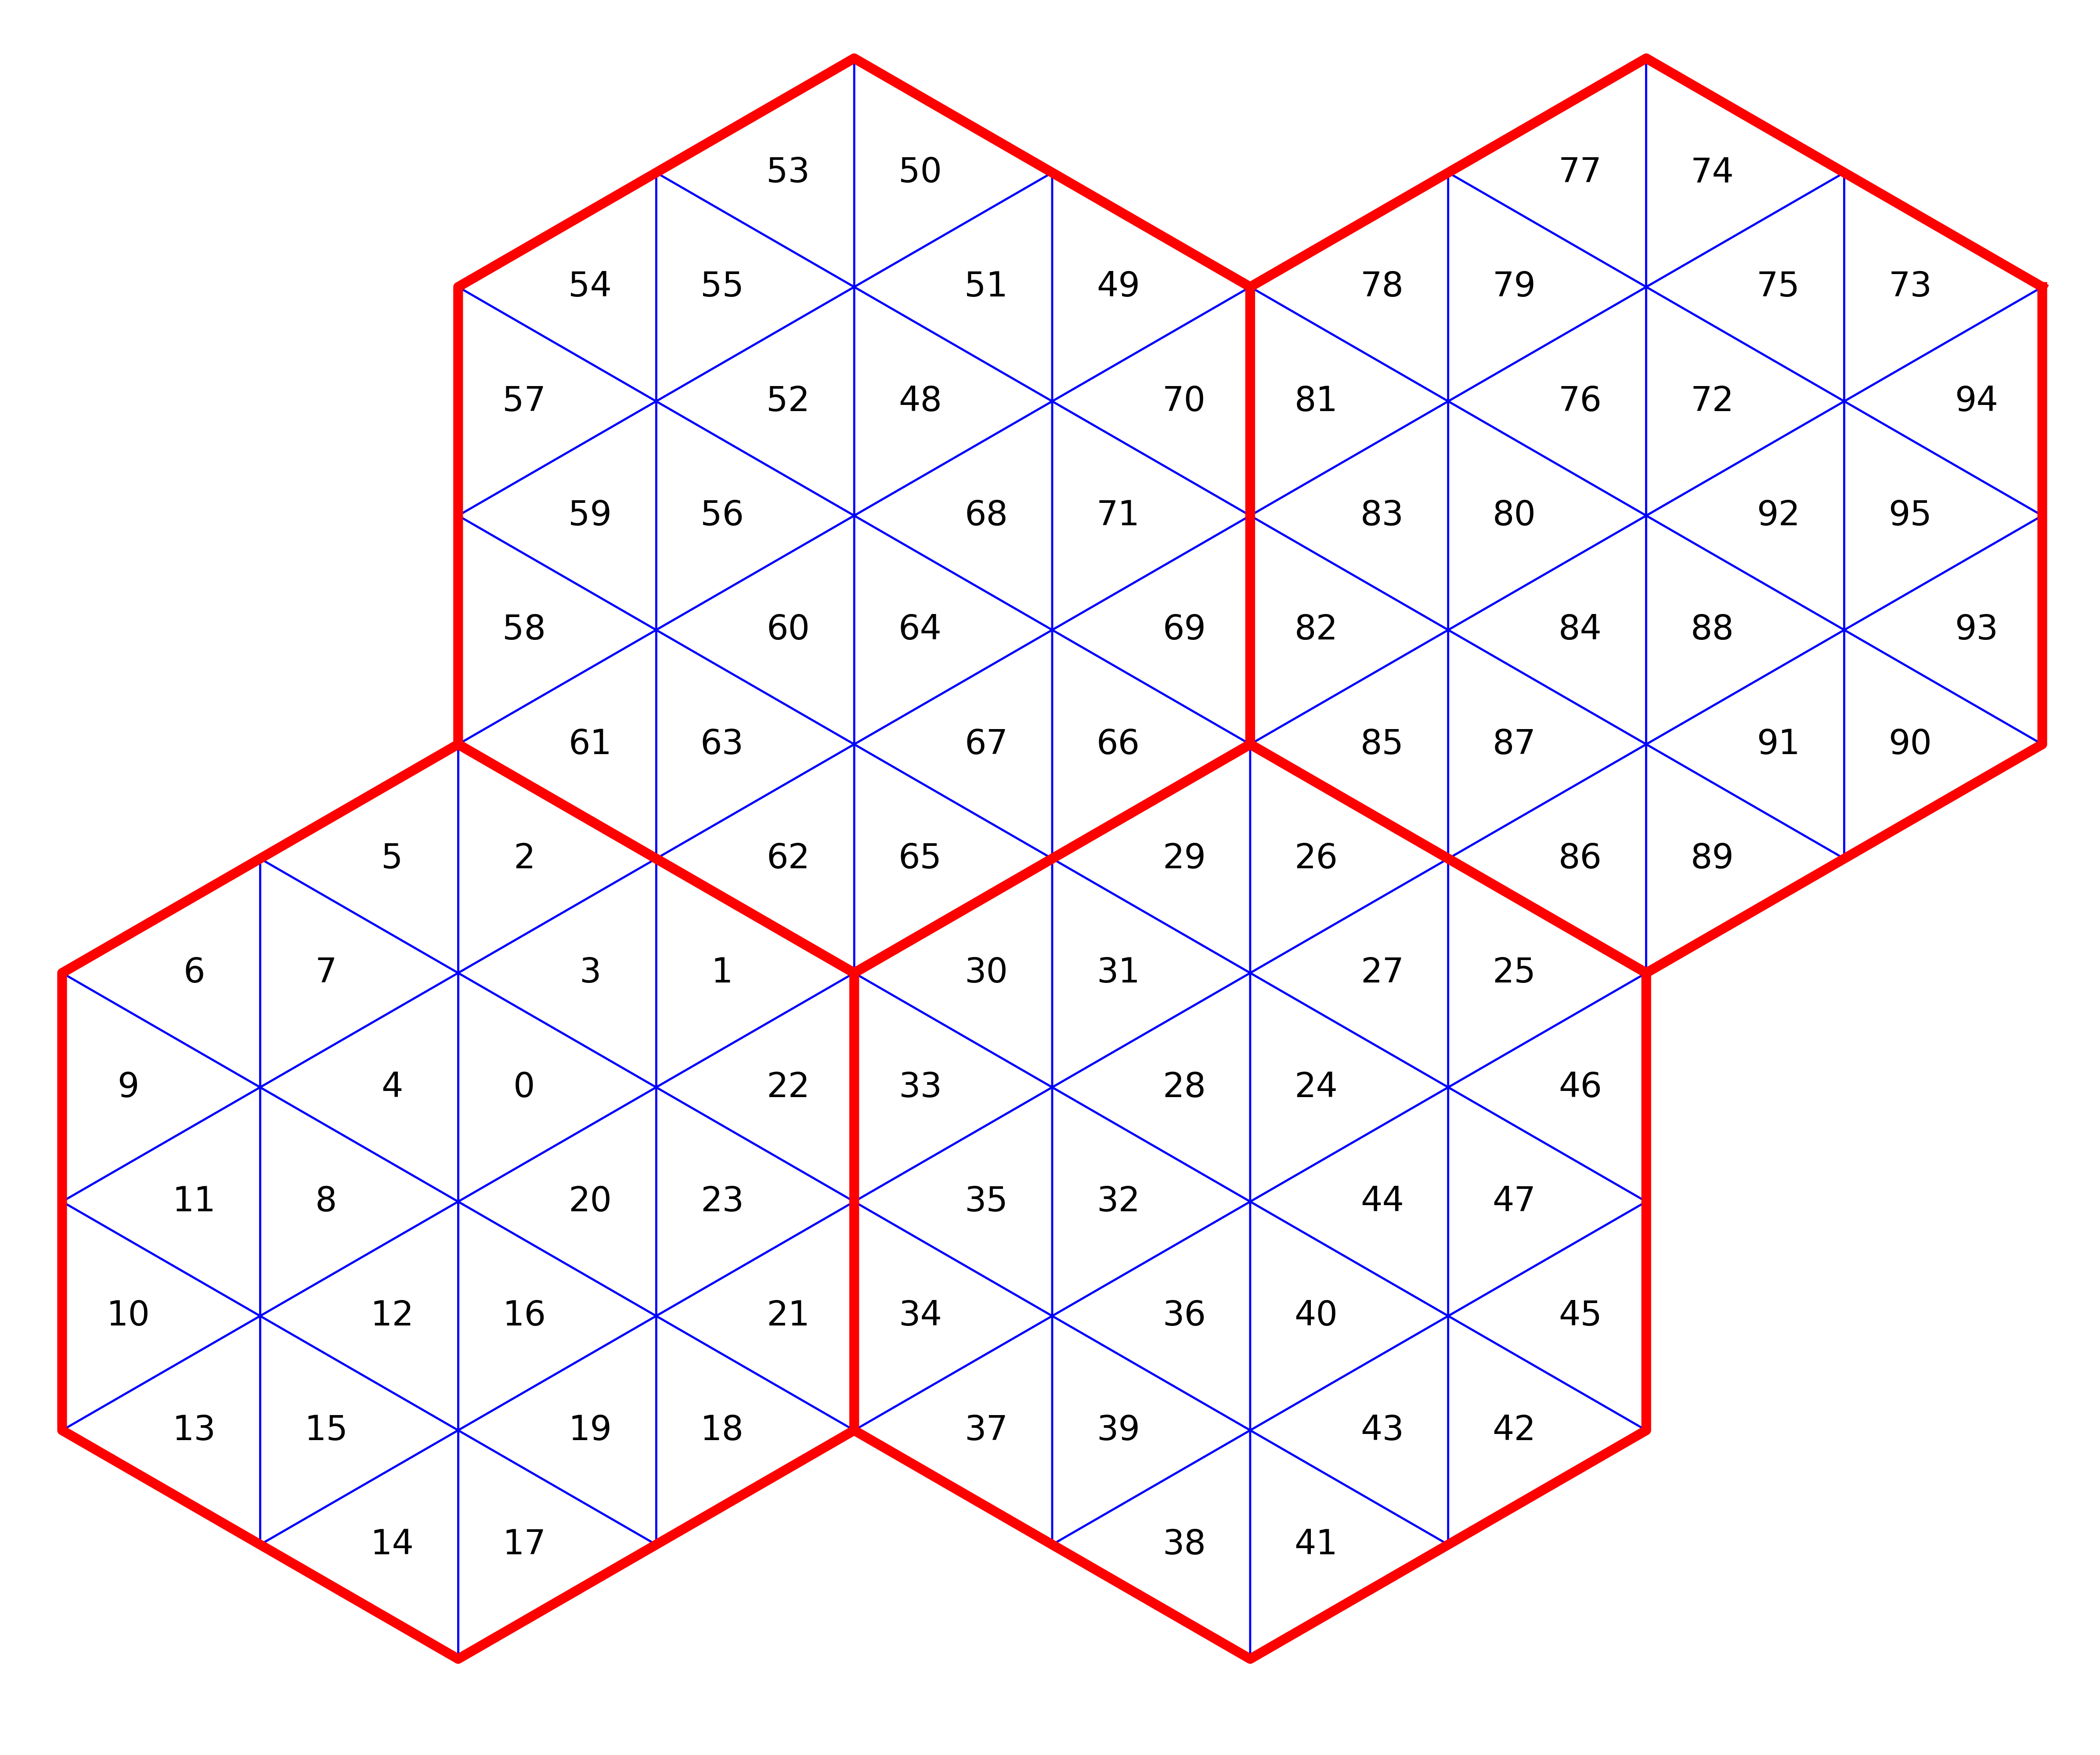
\includegraphics[width=\linewidth]{figures/trial_triangulation_new.png}
        \end{subfigure}
        \caption{2D triangular discretization (left) and hexagon indexing for level 1 (right)}
        \label{fig:2DTri discretization}
\end{figure}
\begin{figure}[H]
        \centering
        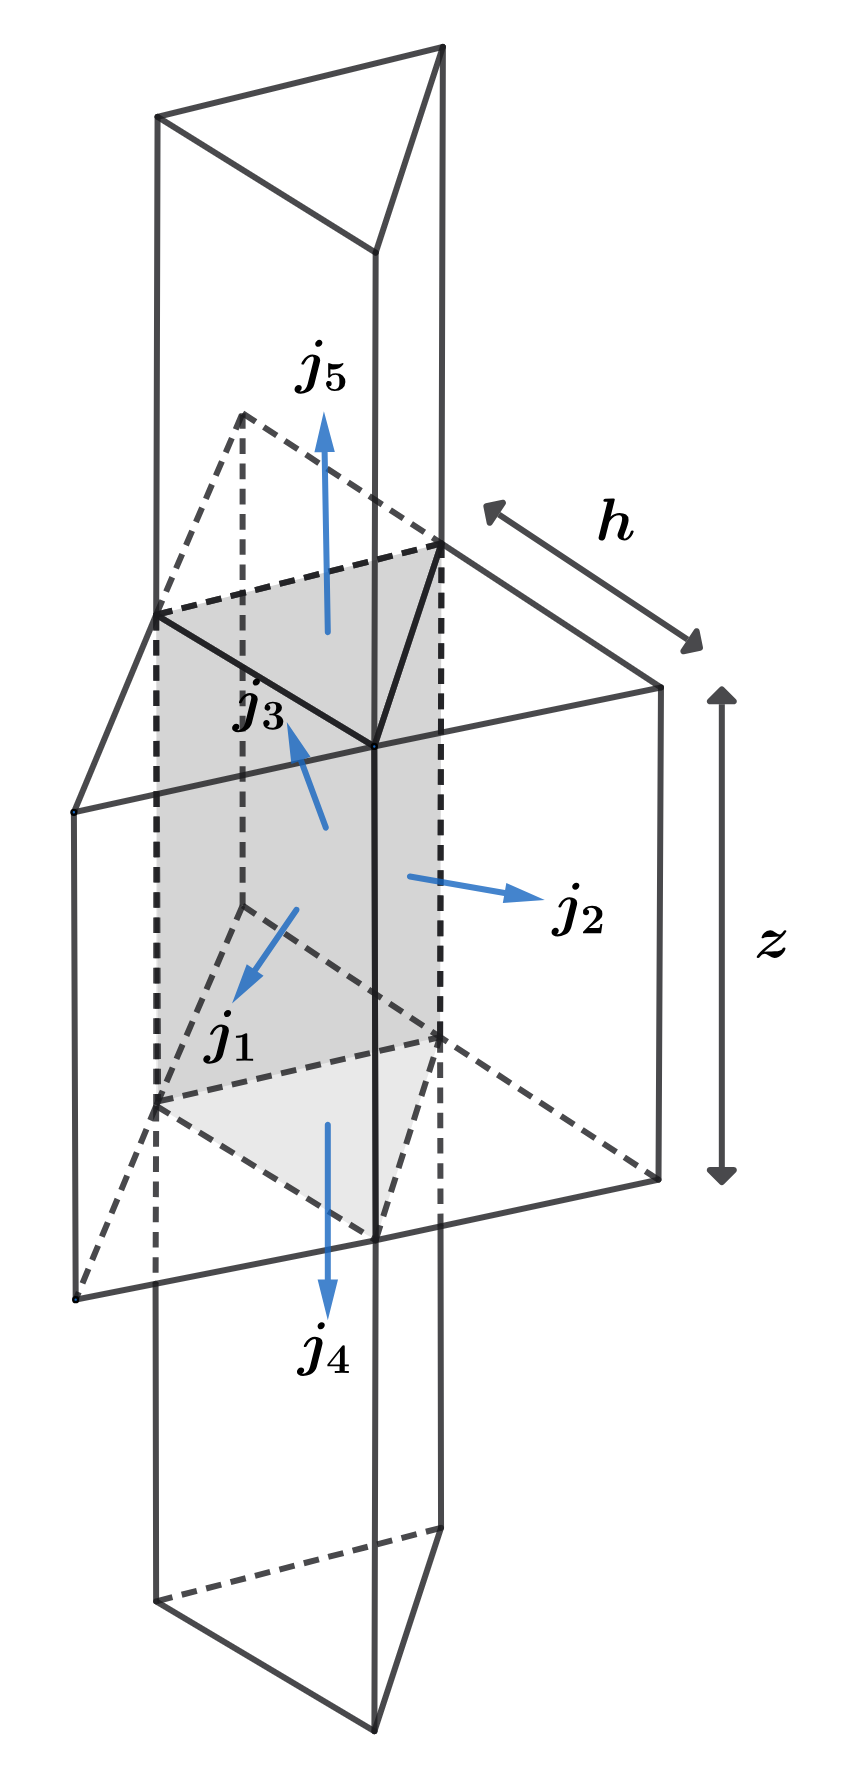
\includegraphics[width=0.35\textwidth]{figures/3DTri_disc2.png}
        \caption{3D discretization of triangular geometries in finite volume method}
        \label{fig:3DTri discretization}
\end{figure}

The discretized form of Eq. \ref{eq:freq_4_ch3} for 3D triangular geometries is as follows:
\begin{equation}
        \begin{aligned}
                \frac{i \omega}{v_g} \delta \phi_{g,i} (\omega) &+ \biggl( \frac{8}{h^2} \biggl( \frac{D_{g,i}D_{g,j1}}{D_{g,i}+D_{g,j1}} + \frac{D_{g,i}D_{g,j2}}{D_{g,i}+D_{g,j2}} + \frac{D_{g,i}D_{g,j3}}{D_{g,i}+D_{g,j3}} \biggr) \delta \phi_{g,i}(\omega) +\\ 
                &\biggl(-\frac{8}{h^2}\frac{D_{g,i}D_{g,j1}}{D_{g,i}+D_{g,j1}}\biggr) \delta \phi_{g,j1}(\omega) + \biggl(-\frac{8}{h^2}\frac{D_{g,i}D_{g,j2}}{D_{g,i}+D_{g,j2}}\biggr) \delta \phi_{g,j2}(\omega) + \biggl(-\frac{8}{h^2}\frac{D_{g,i}D_{g,j3}}{D_{g,i}+D_{g,j3}}\biggr) \delta \phi_{g,j3}(\omega) \biggr) + \\ 
                &\frac{1}{(\Delta z)^2} \biggl( -\frac{2D_{g,i}D_{g,j4}}{D_{g,i}+D_{g,j4}} \delta \phi_{g,j4}(\omega) + \biggl(\frac{2D_{g,i}D_{g,j4}}{D_{g,i}+D_{g,j4}}+\frac{2D_{g,i}D_{g,j5}}{D_{g,i}+D_{g,j5}}\biggr) \delta \phi_{g,i}(\omega) - \\
                &\frac{2D_{g,i}D_{g,j5}}{D_{g,i}+D_{g,j5}} \delta \phi_{g,j5}(\omega) \biggr) + \Sigma_{t,g,i} \delta \phi_{g,i}(\omega) - \sum_{g' = 1}^{G} \biggl(\Sigma_{s0,g',g,i} \delta \phi_{g',i}(\omega) \biggr) - \\
                &\frac{1}{k_{\text{eff}}} \biggl( \chi^p_g (1-\beta_{\text{eff}}) + \chi^d_g \frac{\lambda \beta_{\text{eff}}}{i \omega + \lambda} \biggr)  \biggl(\sum_{g' = 1}^{G} \nu \Sigma_{f,g',i} \delta \phi_{g',i}(\omega) \biggr)= - \delta \Sigma_{t,g,i}(\omega) \phi_{g,i} + \\
                &\sum_{g' = 1}^{G} \biggl(\delta \Sigma_{s0,g',g,i}(\omega) \phi_{g',i}) \biggr) + \frac{1}{k_{\text{eff}}} \biggl( \chi^p_g (1-\beta_{\text{eff}}) + \chi^d_g \frac{\lambda \beta_{\text{eff}}}{i \omega + \lambda} \biggr)  \biggl( \sum_{g' = 1}^{G} \delta \nu \Sigma_{f,g',i}(\omega) \phi_{g',i}) \biggr)
        \end{aligned}
        \label{eq:noise_3D_tri_disc}
\end{equation}

For Eq. \ref{eq:forward_eq_ch3}, the discretization for 3D triangular geometries is as follows:
\begin{equation}
        \begin{aligned}
                \biggl( \frac{8}{h^2} &\biggl( \frac{D_{g,i}D_{g,j1}}{D_{g,i}+D_{g,j1}} + \frac{D_{g,i}D_{g,j2}}{D_{g,i}+D_{g,j2}} + \frac{D_{g,i}D_{g,j3}}{D_{g,i}+D_{g,j3}} \biggr) \phi_{g,i} + \biggl(-\frac{8}{h^2}\frac{D_{g,i}D_{g,j1}}{D_{g,i}+D_{g,j1}}\biggr) \phi_{g,j1} + \\ 
               &\biggl(-\frac{8}{h^2}\frac{D_{g,i}D_{g,j2}}{D_{g,i}+D_{g,j2}}\biggr) \phi_{g,j2} + \biggl(-\frac{8}{h^2}\frac{D_{g,i}D_{g,j3}}{D_{g,i}+D_{g,j3}}\biggr) \phi_{g,j3} \biggr) + \\ 
                &\frac{1}{(\Delta z)^2} \biggl( -\frac{2D_{g,i}D_{g,j4}}{D_{g,i}+D_{g,j4}} \phi_{g,j4} + \biggl(\frac{2D_{g,i}D_{g,j4}}{D_{g,i}+D_{g,j4}}+\frac{2D_{g,i}D_{g,j5}}{D_{g,i}+D_{g,j5}}\biggr) \phi_{g,i} - \\
                &\frac{2D_{g,i}D_{g,j5}}{D_{g,i}+D_{g,j5}} \phi_{g,j5} \biggr) + \Sigma_{t,g,i} \phi_{g,i} =  \sum_{g' = 1}^{G} \biggl(\Sigma_{s0,g',g,i} \phi_{g',i}) \biggr)\\
                & + \frac{1}{k_{\text{eff}}} \biggl( \chi^p_g (1-\beta_{\text{eff}}) + \chi^d_g \frac{\lambda \beta_{\text{eff}}}{i \omega + \lambda} \biggr)  \biggl( \sum_{g' = 1}^{G} \nu \Sigma_{f,g',i} \phi_{g',i}) \biggr)
        \end{aligned}
        \label{eq:forward_3D_tri_disc}
\end{equation}

For Eq. \ref{eq:adjoint_eq_ch3}, the discretization for 3D triangular geometries is as follows:
\begin{equation}
        \begin{aligned}
                \biggl( \frac{8}{h^2} &\biggl( \frac{D_{g,i}D_{g,j1}}{D_{g,i}+D_{g,j1}} + \frac{D_{g,i}D_{g,j2}}{D_{g,i}+D_{g,j2}} + \frac{D_{g,i}D_{g,j3}}{D_{g,i}+D_{g,j3}} \biggr) \phi_{g,i}^{\dagger} + \biggl(-\frac{8}{h^2}\frac{D_{g,i}D_{g,j1}}{D_{g,i}+D_{g,j1}}\biggr) \phi_{g,j1}^{\dagger} + \\ 
               &\biggl(-\frac{8}{h^2}\frac{D_{g,i}D_{g,j2}}{D_{g,i}+D_{g,j2}}\biggr) \phi_{g,j2}^{\dagger} + \biggl(-\frac{8}{h^2}\frac{D_{g,i}D_{g,j3}}{D_{g,i}+D_{g,j3}}\biggr) \phi_{g,j3}^{\dagger} \biggr) + \\ 
                &\frac{1}{(\Delta z)^2} \biggl( -\frac{2D_{g,i}D_{g,j4}}{D_{g,i}+D_{g,j4}} \phi_{g,j4}^{\dagger} + \biggl(\frac{2D_{g,i}D_{g,j4}}{D_{g,i}+D_{g,j4}}+\frac{2D_{g,i}D_{g,j5}}{D_{g,i}+D_{g,j5}}\biggr) \phi_{g,i}^{\dagger} - \\
                &\frac{2D_{g,i}D_{g,j5}}{D_{g,i}+D_{g,j5}} \phi_{g,j5}^{\dagger} \biggr) + \Sigma_{t,g,i} \phi_{g,i}^{\dagger} =  \\
                &\sum_{g' = 1}^{G} \biggl(\Sigma_{s0,g,g',i} \phi_{g',i}^{\dagger} \biggr) + \frac{1}{k_{\text{eff}}} \nu \Sigma_{f,g,i} \biggl( \sum_{g' = 1}^{G} \biggl( \chi^p_{g'} (1-\beta_{\text{eff}}) + \chi^d_{g'} \frac{\lambda \beta_{\text{eff}}}{i \omega + \lambda} \biggr) \phi_{g',i}^{\dagger} \biggr)
        \end{aligned}
        \label{eq:adjoint_3D_tri_disc}
\end{equation}

\subsection{Boundary Conditions}

The boundary conditions implemented here are vacuum, reflective, and zero flux. The vacuum boundary condition is defined as follows,
\begin{equation}
    J_{-}(\textbf{r}_b) = \frac{\phi(\textbf{r}_b)}{4} + \frac{1}{2}D(\textbf{r}_b) \nabla \phi(\textbf{r}_b) = 0
\end{equation}
The reflective boundary condition is defined as follows,
\begin{equation}
    D(\textbf{r}_b) \nabla \phi(\textbf{r}_b) = 0
\end{equation}
For the implementation in the developed tool, the albedo boundary condition is used. The definition of the albedo boundary condition is as follows:
\begin{equation}\label{eq:define_albedo}
    \frac{J_{-}(\textbf{r}_b)}{J_{+}(\textbf{r}_b)} = \alpha
\end{equation}
where $\alpha$ has a range of values between 0 and 1. We can derive Eq. \ref{eq:define_albedo} further as follows:
\begin{equation}
    \begin{aligned}
        J_{-}(\textbf{r}_b) &= \alpha J_{+}(\textbf{r}_b)\\
        \frac{\phi(\textbf{r}_b)}{4} + \frac{1}{2} D(\textbf{r}_b) \nabla \phi(\textbf{r}_b) &= \alpha \biggl( \frac{\phi(\textbf{r}_b)}{4} - \frac{1}{2} D(\textbf{r}_b) \nabla \phi(\textbf{r}_b) \biggr) \\
        (1-\alpha) \frac{\phi(\textbf{r}_b)}{4} + (1+\alpha) \biggl( \frac{1}{2} D(\textbf{r}_b) \nabla \phi(\textbf{r}_b) \biggr) &= 0  \\
        \frac{1-\alpha}{1+\alpha} \frac{\phi(\textbf{r}_b)}{4} + \frac{1}{2} D(\textbf{r}_b) \nabla \phi(\textbf{r}_b) &= 0
    \end{aligned}
\end{equation}
Albedo is a convenient boundary conditions because $\alpha$ = 0 corresponds to the vacuum boundary condition, $\alpha$ = 1 corresponds to reflective boundary condition. Finally, the zero flux boundary condition is defined as follows,
\begin{equation}
    \phi(\textbf{r}_b) = 0
\end{equation}

\subsection{Numerical Methods}

To solve the forward equation (Eq. \ref{eq:forward_eq_ch3}), adjoint equation (Eq. \ref{eq:adjoint_eq_ch3}), and neutron noise equation (Eq. \ref{eq:freq_4_ch3}), we can write those equations in matrix form as follows:
\begin{equation}\label{eq:matrix_forward}
    A_{\text{fw}} \phi_{\text{fw}} = \frac{1}{k_{\text{eff}}} F_{\text{fw}} \phi_{\text{fw}}
\end{equation}
\begin{equation}\label{eq:matrix_adjoint}
    A^{\dagger} \phi^{\dagger} = \frac{1}{k_{\text{eff}}} F^{\dagger} \phi^{\dagger}
\end{equation}
\begin{equation}\label{eq:matrix_noise}
    A_{\text{noise}} \delta \phi_{\text{noise}} = S_{\text{noise}}
\end{equation}
where Eq. \ref{eq:matrix_forward} is the matrix form of forward equation, Eq. \ref{eq:matrix_adjoint} is the matrix from of adjoint equation, and equation \ref{eq:matrix_noise} is the matrix form of neutron noise equation.

In Eq. \ref{eq:matrix_forward}-\ref{eq:matrix_noise}, the coefficient matrices (e.g. $A_{\text{fw}}$, $A^{\dagger}$, and $A_{\text{noise}}$) are large, sparse, and banded. The size of these coefficients is ($\text{G} * N \times \text{G} * N$), where G is the number of neutron energy groups and N is the spatial grid of the system of interest. In this tool, the geometries are discretized using a uniform mesh. Coefficient matrices are constructed using sparse array format. The terms such as $D$, $\Sigma_t$,$\Sigma_s$, and $\nu \Sigma_f$ are constructed separately. Then, the operators are combined into the coefficient matrices. 

Since we are solving a sparse system of equations in Eqs. \ref{eq:matrix_forward}-\ref{eq:matrix_noise}, it is beneficial to use a sparse matrix solver. In this tool, the sparse matrix solver is obtained from the PETSc (Portable, Extensible Toolkit for Scientific Computation) Library. PETSc is a suite of algorithms and data structures for the solution of problems arising in scientific and engineering applications, especially those modeled by partial differential equation, and targeted for high performance parallel computing environments \cite{dalcinParallelDistributedComputing2011}. PETSc includes a large suite of scalable parallel linear and nonlinear equation solvers, ODE integrators, and optimization algorithms for application codes written in C, C++, Fortran, and Python \cite{balayPETScTAOUsers2025}.

The matrix solver in this tool is divided into two categories, the eigenvalue solver and fixed source solver. The eigenvalue solver is used to solve forward and adjoint equations, while the fixed source solver is used to solve the neutron noise equation. For all the matrix solvers, the tool applies the iterative Generalized Minimal Residual (GMRES) method. The acceleration of the convergence is obtained from a preconditioner, which can be chosen between Incomplete LU (ILU) and LU preconditioner. The eigenvalue problem is solved using the standard power iteration method, while the fixed source problem is solved with a conventional linear system solver.

\section{Simulated Cases for Verification Purposes}
\label{sec:simulated_vandv}

\subsection{2D Homogeneous Reactor}

In this case, simulations were performed and compared with the analytical solutions based on an infinitely long homogeneous cylindrical reactor with radius 150 cm. For the simulations, the cylinder is approximated using triangular meshes. There are 19,692 triangular meshes in this case. A vacuum boundary condition is assumed on all sides of the reactor. The homogeneous macroscopic cross-sections, the diffusion coefficients, and the kinetic parameters are given in Table \ref{table:2DHomogParam}. 

\begin{table}[H]
\centering
\caption{Kinetic parameters and cross-sections of 2D Homogeneous Reactor in Triangular Grid}
\label{table:2DHomogParam}

% Define custom color
\definecolor{myyellow}{RGB}{255, 255, 150}

\renewcommand{\arraystretch}{1.0} % row height

\begin{tabular}{|>{\centering\arraybackslash}m{3cm}|>{\centering\arraybackslash}m{3cm}|>{\centering\arraybackslash}m{3cm}|}
\hline
\textbf{Parameter} & \textbf{Value} & \textbf{Unit} \\ \hline
\rowcolor{myyellow}\multicolumn{3}{|c|}{\textbf{Kinetic Parameters}} \\ \hline
$\beta_{\text{eff}}$ & 535 & pcm \\ \hline
$\lambda$ & 0.085 & $s^{-1}$ \\ \hline
$v_1$ & 18372300 & cm/s \\ \hline
$v_2$ & 413086 & cm/s \\ \hline

\rowcolor{myyellow}\multicolumn{3}{|c|}{\textbf{Cross-sections}} \\ \hline
$\Sigma_{a,1} $ & 0.0115 & $cm^{-1}$ \\ \hline
$\Sigma_{a,2} $ & 0.1019 & $cm^{-1}$ \\ \hline
$\nu \Sigma_{f,1} $ & 0.0057 & $cm^{-1}$ \\ \hline
$\nu \Sigma_{f,2} $ & 0.14425 & $cm^{-1}$ \\ \hline
$\Sigma_{R} $ & 0.0151 & $cm^{-1}$ \\ \hline
$D_1$ & 0.5376 & cm \\ \hline
$D_2$ & 0.1423 & cm \\ \hline

\end{tabular}
\end{table}

\subsubsection{Forward Flux Solution}

For the forward flux, the analytical solution is described in Eq. \ref{eq:2DHomog_forward_ana}.
\begin{equation}\label{eq:2DHomog_forward_ana}
    \begin{bmatrix}
        \phi_1(r) \\[4pt]
        \phi_2(r)
    \end{bmatrix}
    =
    \begin{bmatrix}
    1 \\[4pt]
    c_\mu
    \end{bmatrix}
    J_0\!\big(B_g r\big)
\end{equation}
where,
\begin{equation}
    \begin{aligned}
        B_g^2 &= \biggl( \frac{j_0}{R + 2D_1} \biggr)^2 \\
        c_{\mu} &= \frac{\Sigma_R}{\Sigma_{a,2} + D_2 B_g^2}
    \end{aligned}
\end{equation}
$j_0$ is the first root of the Bessel function $J_0$.

The analytical $k_{\text{eff}}$ is calculated using Eq. \ref{eq:2DHomog_forward_ana_keff}.
\begin{equation}
    k_{\text{eff}} = \frac{\nu \Sigma_{f,2} \Sigma_R + \nu \Sigma_{f,1} (\Sigma_{a,2} + D_2 B_g^2)}{(\Sigma_{a,1} + D_1 B_g^2 + \Sigma_R) (\Sigma_{a,2} + D_2 B_g^2)}
    \label{eq:2DHomog_forward_ana_keff}
\end{equation}

The comparison between the tool and the analytical solutions are described in Table \ref{table:2DHomog_fw_results} and Figure \ref{fig:2DHomog_fw_results_compare}.

\begin{table}[H]
        \centering
        \caption{Eigenvalue comparison of 2D Homogeneous Reactor}
        \label{table:2DHomog_fw_results}
        \begin{tabular}{ | M{3.5cm} | M{2cm} | } 
         \hline
         $k_{\text{eff}}$ Analytical & 1.01241  \\
         \hline
         $k_{\text{eff}}$ tool & 1.01241  \\
         \hline
         Absolute Error (pcm) & 0.0  \\
         \hline
        \end{tabular}
\end{table}

\begin{figure}[H]
        \centering
        \begin{subfigure}{.48\textwidth}
          \centering
          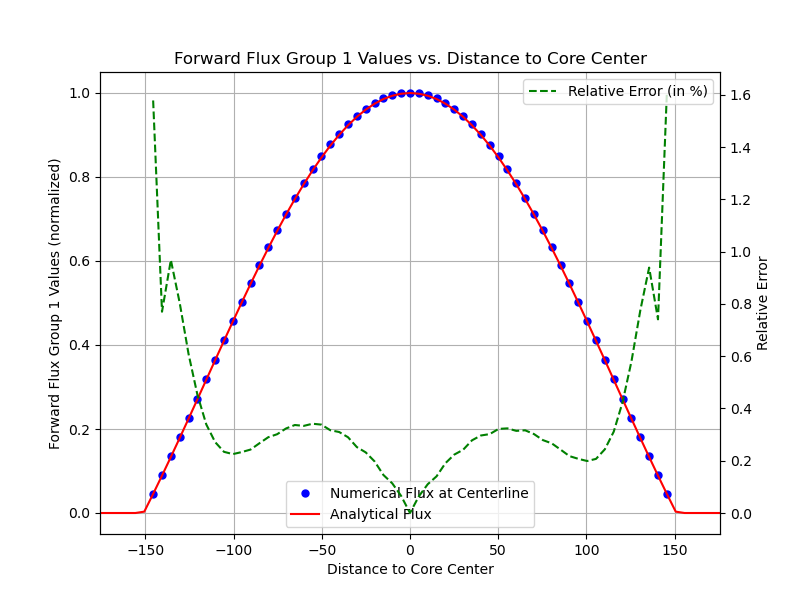
\includegraphics[width=\linewidth]{figures/Verification_PHI_magnitude_G1.png}
        \end{subfigure}
        \hfill
        \begin{subfigure}{.48\textwidth}
          \centering
          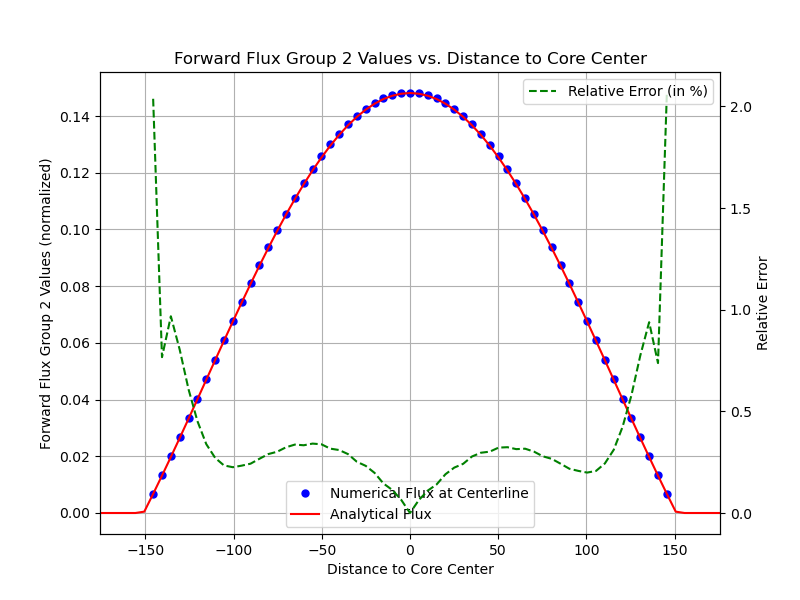
\includegraphics[width=\linewidth]{figures/Verification_PHI_magnitude_G2.png}
        \end{subfigure}
        \caption{Comparison of forward flux at the centerline between the tool and analytical solutions}
        \label{fig:2DHomog_fw_results_compare}
\end{figure}

The results show that the tool agrees well with the analytical solutions of the forward flux, with a maximum error of 2\% at the periphery of the core. The $k_{\text{eff}}$ matches between analytical solution and the developed tool. This demonstrates that the tool performs effectively for 2D triangular geometries.

\subsubsection{Adjoint Flux Solution}

For the adjoint flux, the analytical solution is described in Eq. \ref{eq:2DHomog_adjoint_ana}.
\begin{equation}\label{eq:2DHomog_adjoint_ana}
    \begin{bmatrix}
        \phi_1^{\dagger}(r) \\[4pt]
        \phi_2^{\dagger}(r)
    \end{bmatrix}
    =
    \begin{bmatrix}
    1 \\[4pt]
    c_\mu^{\dagger}
    \end{bmatrix}
    J_0\!\big(B_g r\big)
\end{equation}
where,
\begin{equation}
    \begin{aligned}
        c_{\mu}^{\dagger} &= \frac{1}{k_\text{eff}} \frac{\nu \Sigma_{f,2}}{\Sigma_{a,2} + D_2 B_g^2}
    \end{aligned}
\end{equation}

The comparison between the tool and the analytical solutions are described in Figure \ref{fig:2DHomog_adj_results_compare}.

\begin{figure}[H]
        \centering
        \begin{subfigure}{.48\textwidth}
          \centering
          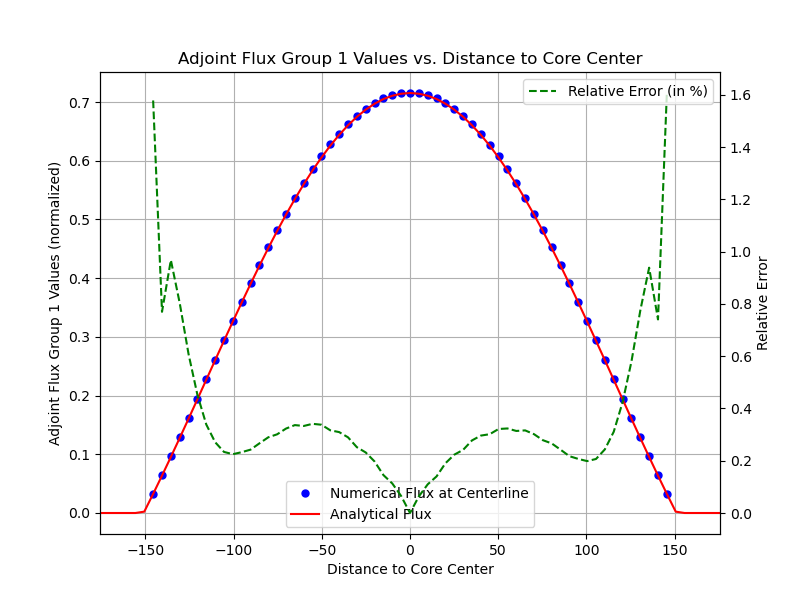
\includegraphics[width=\linewidth]{figures/Verification_PHI_ADJ_magnitude_G1.png}
        \end{subfigure}
        \hfill
        \begin{subfigure}{.48\textwidth}
          \centering
          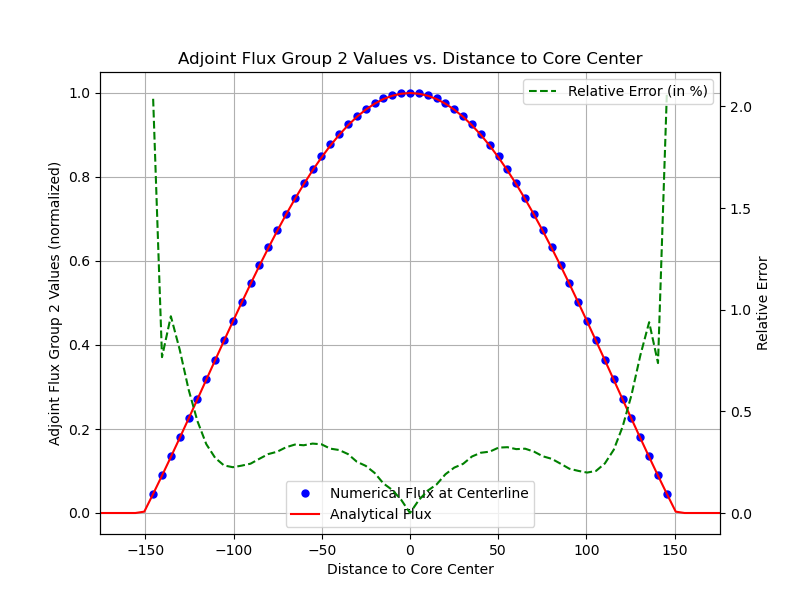
\includegraphics[width=\linewidth]{figures/Verification_PHI_ADJ_magnitude_G2.png}
        \end{subfigure}
        \caption{Comparison of adjoint flux at the centerline between the tool and analytical solutions}
        \label{fig:2DHomog_adj_results_compare}
\end{figure}

The results show that the tool agrees well with the analytical solutions of the adjoint flux, with a maximum error of 2\% at the periphery of the core. This indicates that the tool performs effectively for 2D triangular geometries.

\subsubsection{Neutron Noise Solution}

In this case, it is defined that the noise source perturbed the absorption cross-section.
\begin{equation}
    \delta \Sigma_{a,2}(\textbf{r}_p,\omega) = 0.3
\end{equation}

where we define $\textbf{r}_p$ at the center of the core with a frequency of 1 Hz. The analytical solutio for this problem is described in Eq. \ref{eq:2DHomog_noise_ana}.
\begin{equation}\label{eq:2DHomog_noise_ana}
    \begin{bmatrix}
       \delta \phi_1(r, \omega) \\[4pt]
       \delta \phi_2(r, \omega)
    \end{bmatrix}
    = \frac{1}{4 D_2(c_\lambda - c_\mu)}
    \begin{bmatrix}
        1 \\[4pt]
        c_\mu
    \end{bmatrix}
    \biggl(J_0(\mu r) \frac{Y_0(\mu R)}{J_0(\mu R)} - Y_0(\mu r) \biggr) - \frac{1}{2 \pi D_2(c_\lambda - c_\mu)}
    \begin{bmatrix}
        1 \\[4pt]
        c_\lambda
    \end{bmatrix}
    \biggl(K_0(\lambda r) - I_0(\lambda r) \frac{K_0(\lambda R)}{I_0(\lambda R)} \biggr) 
\end{equation}
where,
\begin{equation}
    \begin{aligned}
        \mu^2 &= \frac{-(\Sigma_1 D_2 + \Sigma_2 D_1) + \sqrt{(\Sigma_1 D_2 + \Sigma_2 D_1)^2 -4 D_1 D_2 (\Sigma_1 \Sigma_2 - \Sigma_R \nu \Sigma_{f,2}}}{2 D_1 D_2} \\
        \lambda^2 &= \frac{(\Sigma_1 D_2 + \Sigma_2 D_1) + \sqrt{(\Sigma_1 D_2 + \Sigma_2 D_1)^2 -4 D_1 D_2 (\Sigma_1 \Sigma_2 - \Sigma_R \nu \Sigma_{f,2}}}{2 D_1 D_2} \\
        c_\mu &= \frac{\Sigma_R}{\Sigma_2 + D_2 \mu^2} \\
        c_\lambda &= \frac{\Sigma_R}{\Sigma_2 - D_2 \lambda^2} \\
        \Sigma_1 &= \Sigma_{a,1} + \frac{i\omega}{v_1} + \Sigma_R - \nu \Sigma_{f,1} \\
        \Sigma_2 &= \Sigma_{a,2} + \frac{i\omega}{v_2}
    \end{aligned}
\end{equation}

The comparison between the developed tool and analytical solutions are described in Figure \ref{fig:2DHomog_noise_results_diff_phi}

\begin{figure}[H]
        \centering
        \begin{subfigure}{.48\textwidth}
          \centering
          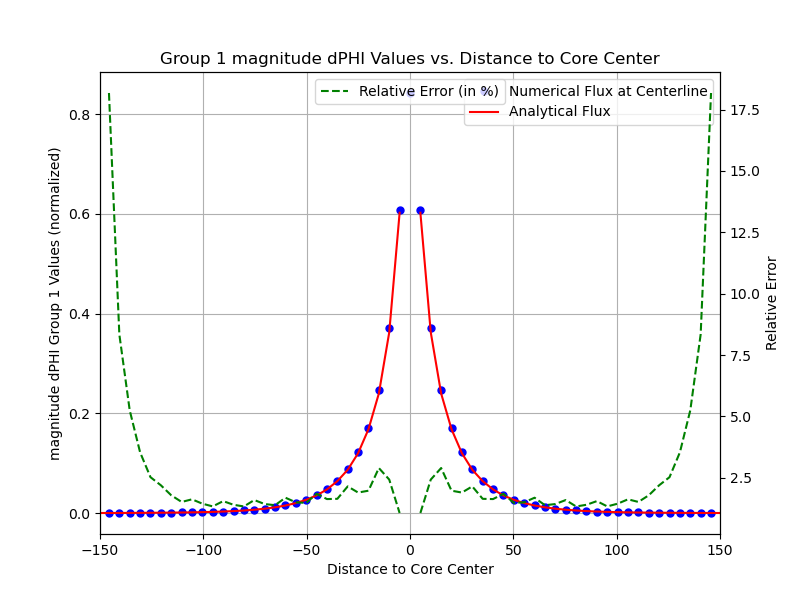
\includegraphics[width=\linewidth]{figures/Verification_dPHI_magnitude_G1.png}
        \end{subfigure}
        \hfill
        \begin{subfigure}{.48\textwidth}
          \centering
          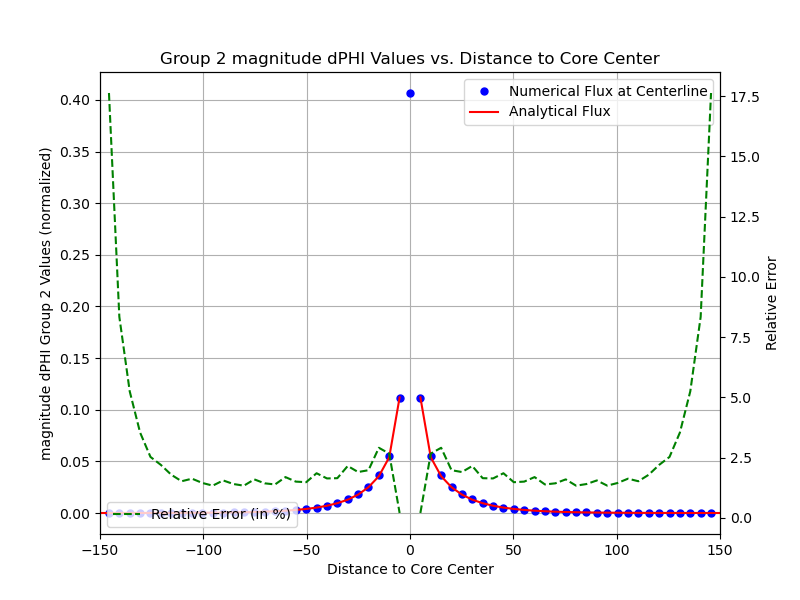
\includegraphics[width=\linewidth]{figures/Verification_dPHI_magnitude_G2.png}
        \end{subfigure}
\end{figure}
\begin{figure}[H]\ContinuedFloat
        \centering
        \begin{subfigure}{.48\textwidth}
          \centering
          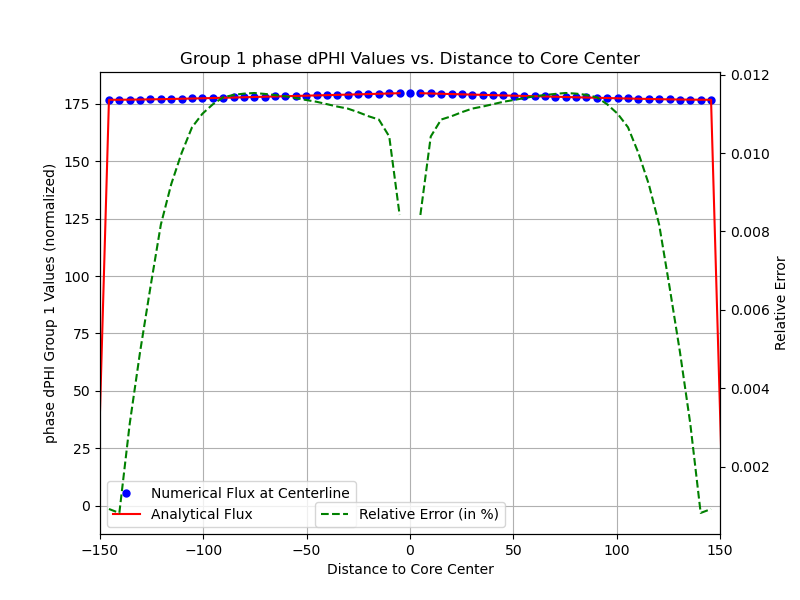
\includegraphics[width=\linewidth]{figures/Verification_dPHI_phase_G1.png}
        \end{subfigure}
        \hfill
        \begin{subfigure}{.48\textwidth}
          \centering
          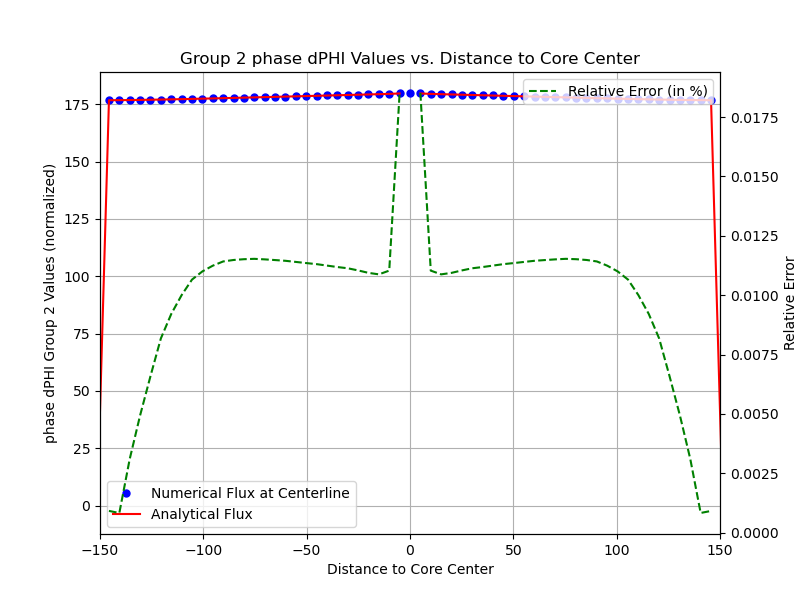
\includegraphics[width=\linewidth]{figures/Verification_dPHI_phase_G2.png}
        \end{subfigure}
        \caption{Comparison of neutron noise at the centerline between the developed tool and analytical solutions}
        \label{fig:2DHomog_noise_results_diff_phi}
\end{figure}

The results show that the solutions for both magnitude and phase in each group agree well with the analytical solution. Since the noise source is defined as perturbations in $\Sigma_{a,2}$, the noise in group 2 reaches its peak at the center of the core. The relative error is higher in the periphery, which is similar to previous cases, due to the neutron noise value being close to zero but still within a reasonable range. Overall, the tool works well compared to the analytical solutions.

\subsection{2D VVER-400 Benchmark}

The VVER-400 Benchmark is developed from \cite{chaoConformalMappingHexagonal1995} to simulate the capability for hexagonal geometries. The VVER-440-type reactor core design features large control rod assemblies that do not contain fuel rods. As a control rod assembly moves into the core, it pushes the fuel assembly underneath out of the way. This results in a significant flux gradient near the interfaces of the control rod assembly and its neighboring fuel assemblies. The core consists of 312 standard fuel assemblies, 37 control assemblies, and a layer of reflector assemblies surrounding the core boundary. The fuel assembly pitch is 14.7 cm. A vacuum boundary condition was applied to the outer boundary of the reflector. In this section, the forward flux is simulated and compared with FEMFFUSION, a finite element-based code developed by Universitat Politècnica de València \cite{vidal-ferrandizFEMFFUSIONFiniteElement2023}. To calculate the error, the normalized power in each assembly is used as the parameter to compare \cite{vidal-ferrandizMovingMeshesSolve2016}. To calculate the normalized power in each assembly, first we define the power for each mesh point $i$ ($P_i$) as follows:
\begin{equation}
    P_i = E_R \sum_g \Sigma_{f,i,g} \phi_{i,g} V_i
\end{equation}
where $E_R$ is the recoverable energy per fission, which is assumed to be constant, and $V_i$ is the volume of the mesh. Then, the normalized power for each assembly $k$ ($P_k$) is defined as follows:
\begin{equation}
    P_k = \frac{\sum_{i=1}^I P_i}{V_k}
\end{equation}
where $I$ is the number of mesh points in one assembly, and $V_k$ is the volume of the assembly. The relative error is calculated as follows:
\begin{equation}
    \varepsilon_k = \frac{|P_{k, \text{calc}}-P_{k, \text{ref}}|}{|P_{k, \text{ref}}|}
\end{equation}

\subsubsection{Forward Flux Solution}

For the tool, the hexagon is divided into six triangular mesh. The eigenvalue comparison is in Table \ref{table:2DVVER_fw_results}, while forward flux and the forward flux comparison to FEMFFUSION are in Figure \ref{fig:2DVVER_fw_results_flx} - \ref{fig:2DVVER_fw_results_diff_phi}.

\begin{table}[H]
        \centering
        \caption{Eigenvalue comparison of 2D VVER-400}
        \label{table:2DVVER_fw_results}
        \begin{tabular}{ | M{3.5cm} | M{2cm} | } 
         \hline
         $k_{\text{eff}}$ FEMFFUSION & 1.003495  \\
         \hline
         $k_{\text{eff}}$ tool & 1.002570  \\
         \hline
         Absolute Error (pcm) & 92.5  \\
         \hline
        \end{tabular}
\end{table}

\begin{figure}[H]
        \centering
        \begin{subfigure}{.48\textwidth}
          \centering
          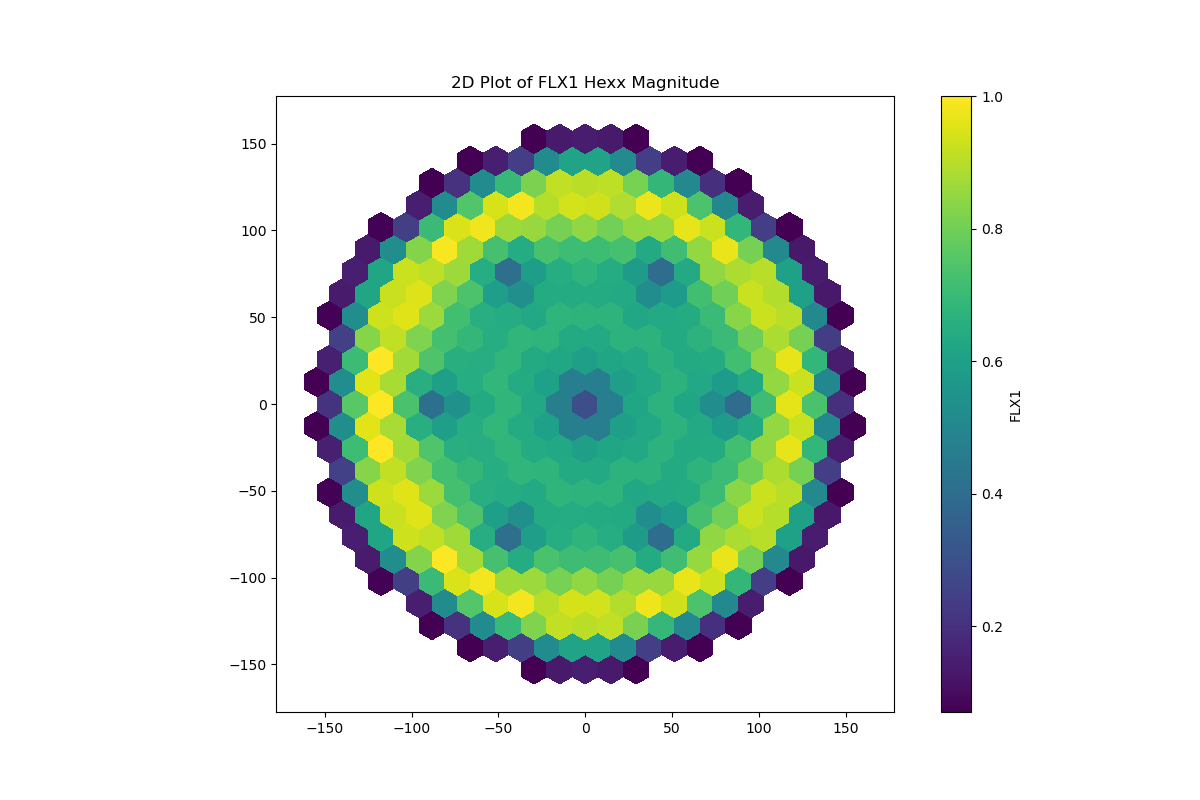
\includegraphics[width=\linewidth]{figures/OBJECTIVES1_TEST05_2DTriMG_VVER400_VandV_level2_FORWARD_FLX_magnitude_G1.png}
        \end{subfigure}
        \hfill
        \begin{subfigure}{.48\textwidth}
          \centering
          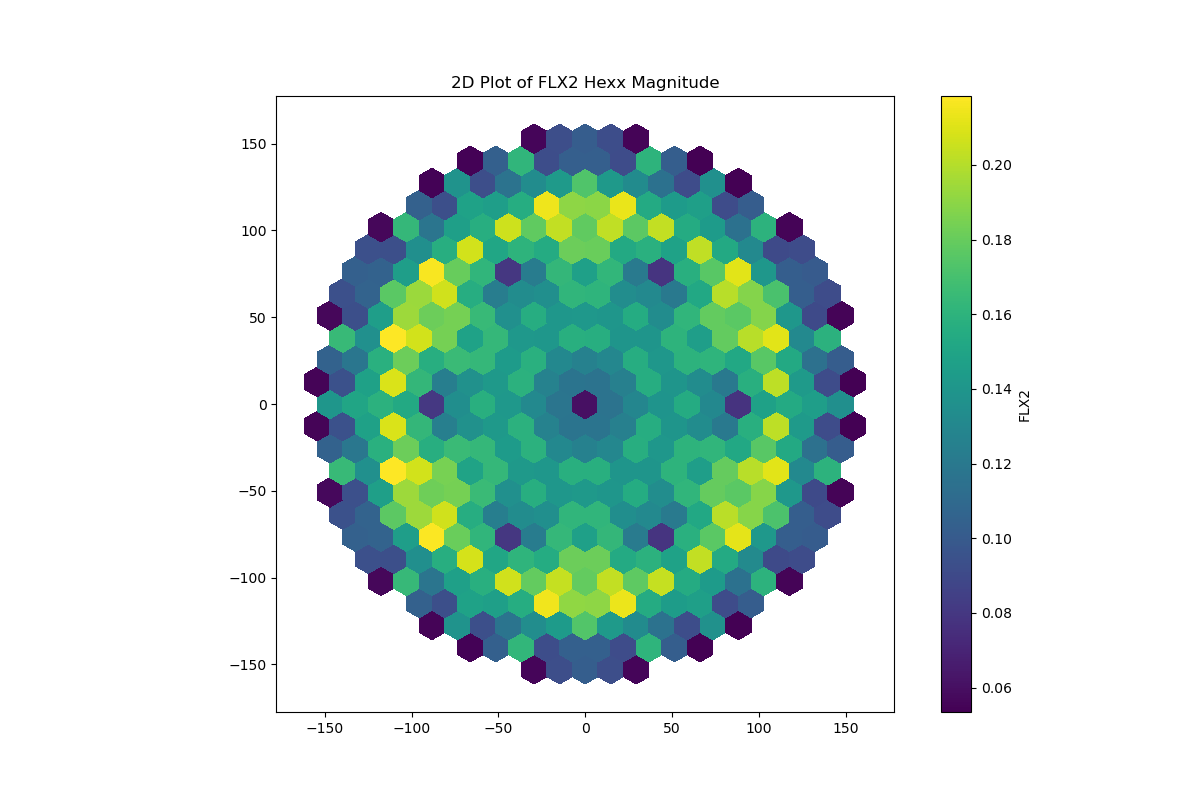
\includegraphics[width=\linewidth]{figures/OBJECTIVES1_TEST05_2DTriMG_VVER400_VandV_level2_FORWARD_FLX_magnitude_G2.png}
        \end{subfigure}
        \caption{Forward flux results from FEMFFUSION}
        \label{fig:2DVVER_fw_results_flx}
\end{figure}
\begin{figure}[H]
        \centering
        \begin{subfigure}{.48\textwidth}
          \centering
          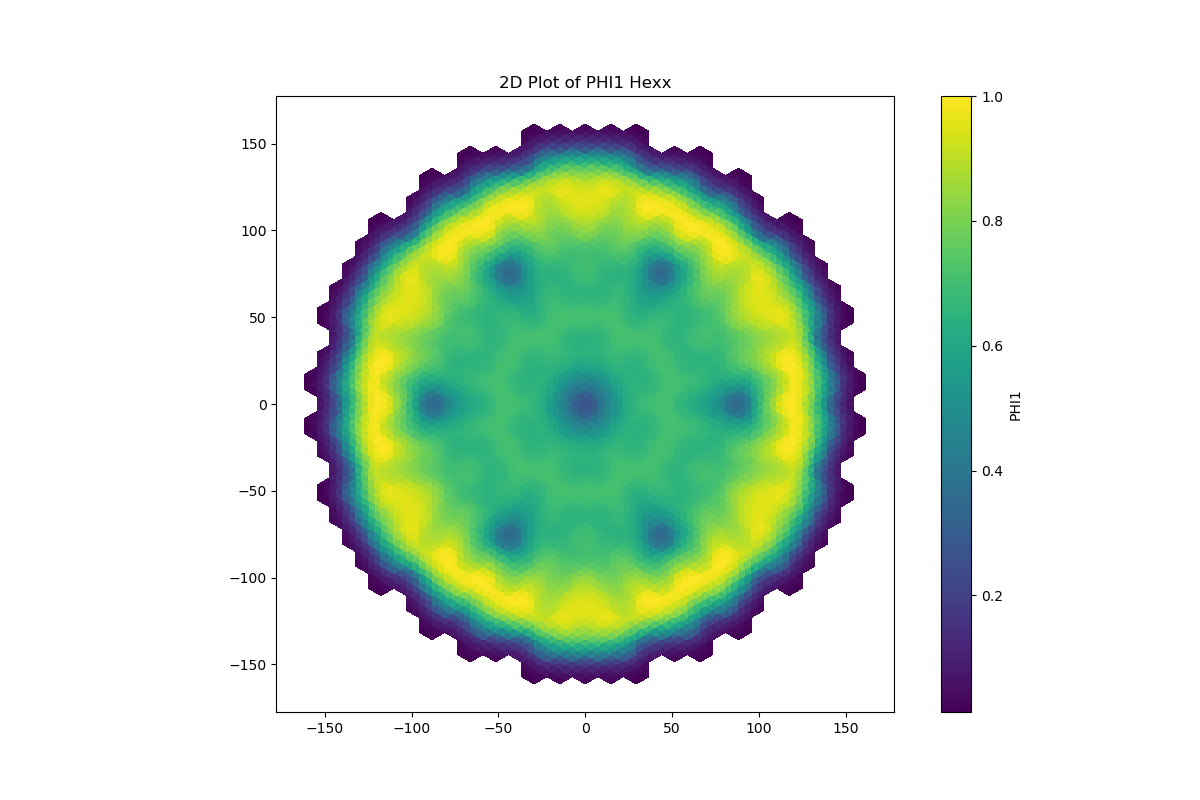
\includegraphics[width=\linewidth]{figures/OBJECTIVES1_TEST05_2DTriMG_VVER400_VandV_level2_FORWARD_PHI_magnitude_G1.png}
        \end{subfigure}
        \hfill
        \begin{subfigure}{.48\textwidth}
          \centering
          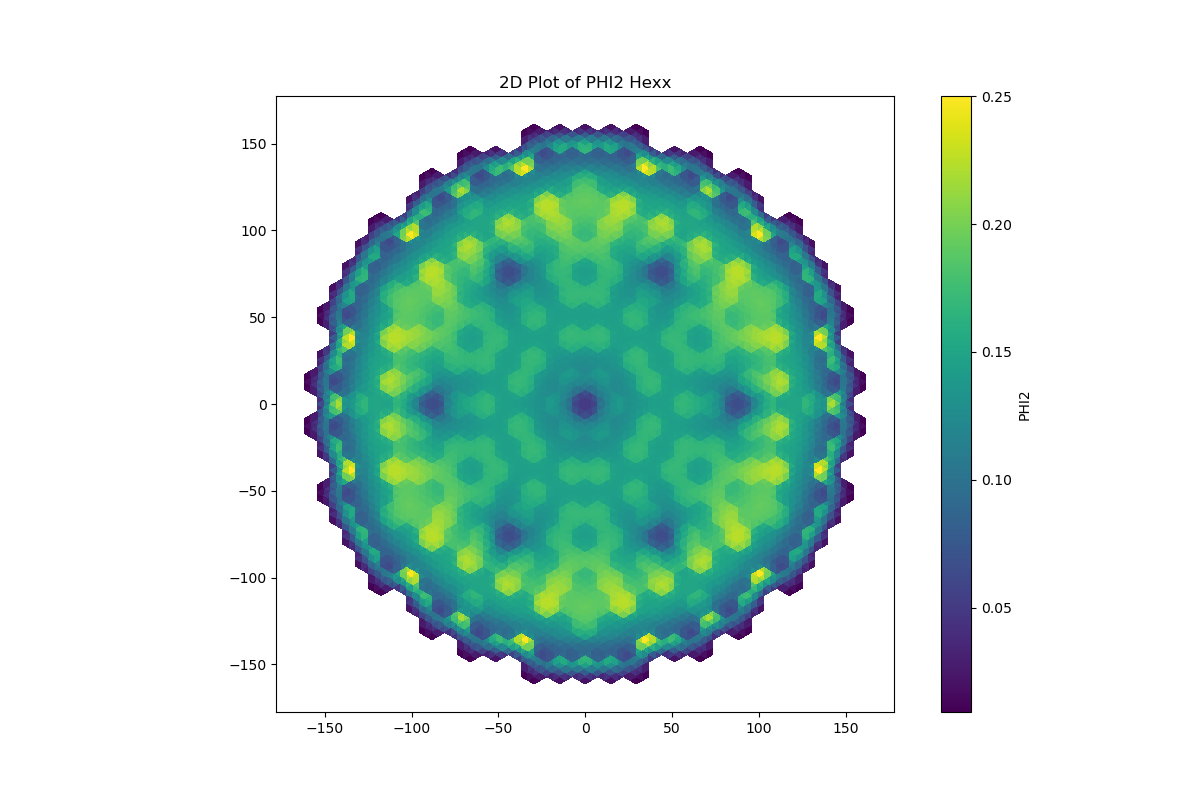
\includegraphics[width=\linewidth]{figures/OBJECTIVES1_TEST05_2DTriMG_VVER400_VandV_level2_FORWARD_PHI_magnitude_G2.png}
        \end{subfigure}
        \caption{Forward flux results from the developed tool}
        \label{fig:2DVVER_fw_results_phi}
\end{figure}
\begin{figure}[H]
        \centering
        \begin{subfigure}{.48\textwidth}
          \centering
          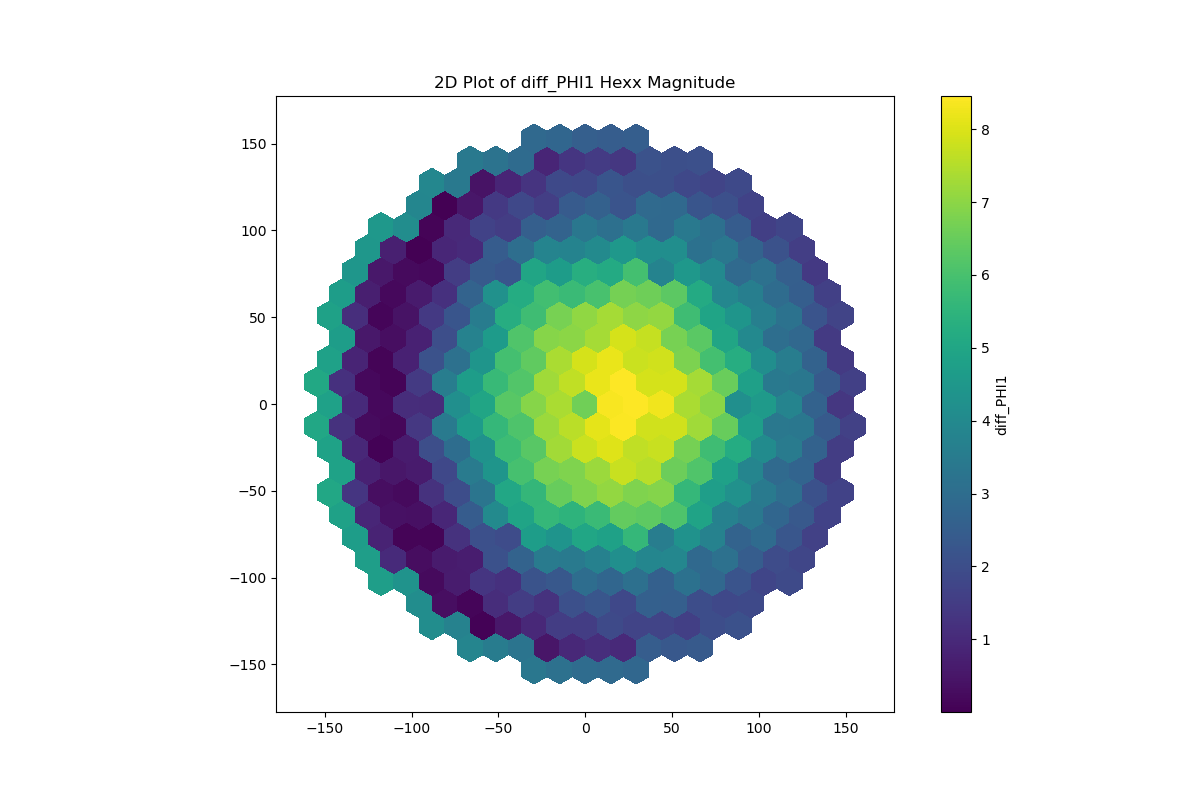
\includegraphics[width=\linewidth]{figures/OBJECTIVES1_TEST05_2DTriMG_VVER400_VandV_level2_FORWARD_diff_PHI_magnitude_G1.png}
        \end{subfigure}
        \hfill
        \begin{subfigure}{.48\textwidth}
          \centering
          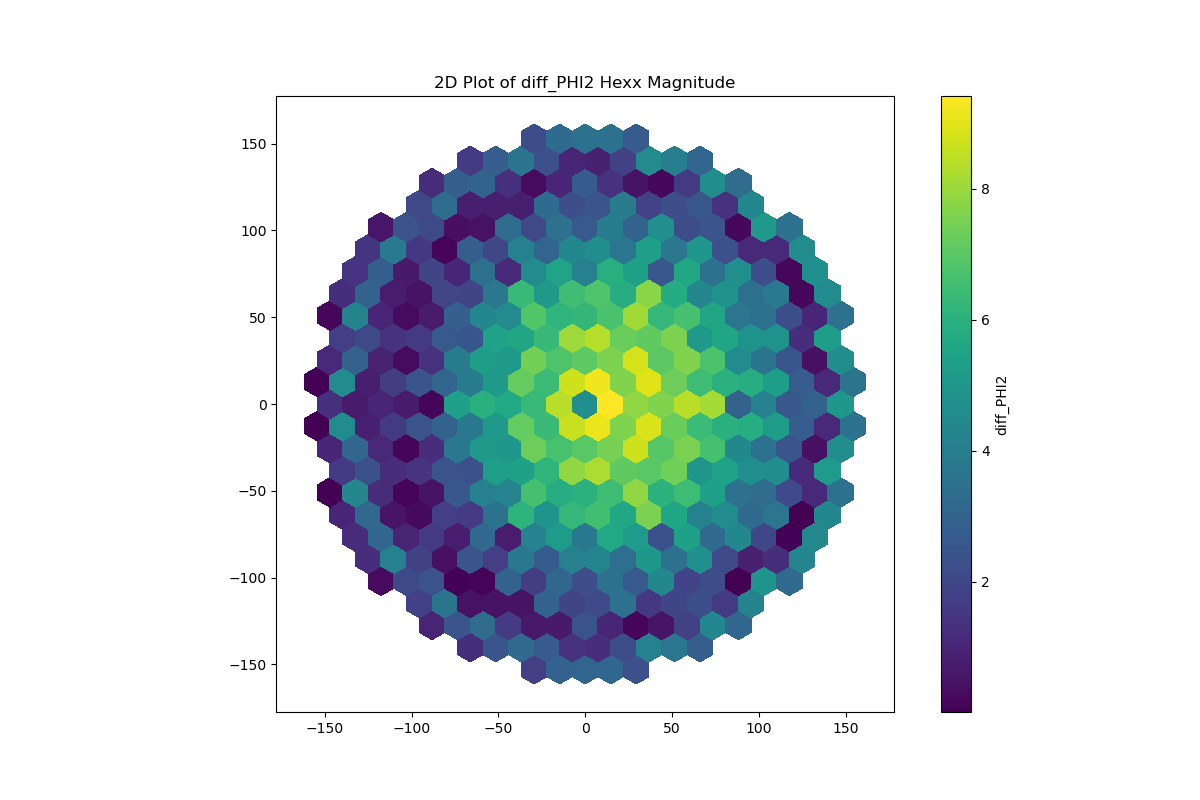
\includegraphics[width=\linewidth]{figures/OBJECTIVES1_TEST05_2DTriMG_VVER400_VandV_level2_FORWARD_diff_PHI_magnitude_G2.png}
        \end{subfigure}
        \caption{Difference of forward flux between FEMFFUSION and the tool}
        \label{fig:2DVVER_fw_results_diff_phi}
\end{figure}

The results show a good agreement between the tool and FEMFFUSION, with a maximum error of 8\% in the forward flux. Overall, the tool is in good agreement with FEMFFUSION.

\section{Conclusion}

A numerical tool has been developed for neutron noise application. The tool is based on the 3-dimensional, multigroup neutron diffusion equation in the frequency domain. The tool can solve rectangular and hexagonal geometries. The tool is designed to solve forward, adjoint, and neutron noise equations with two types of neutron noise sources. It uses sparse matrices to solve systems of linear equations obtained from PETSc. Several cases have been simulated to verify the numerical results against analytical solutions, as well as other tools, such as FEMFFUSION. The results demonstrate that the developed tool aligns with those from analytical solutions and other numerical tools. 


\chapter{Neutron Noise Simulation of High Temperature Test Reactor (HTTR)}
\label{ch:noise_HTTR}

Efforts to deploy advanced reactors are actively ongoing in many countries. The types of reactors vary, including High-Temperature Gas-cooled reactors (HTGRs), Molten Salt Reactors (MSRs), Lead-Cooled Fast Reactors (LFRs), Sodium Fast Reactors (SFRs), and many more \cite{pioroHandbookGenerationIV2016}. With the massive development of advanced reactors, advancements in core monitoring and diagnostics for advanced reactors are expected. On the other hand, the development of autonomous or semi-autonomous reactor control is on the rise. These imply that core monitoring and diagnostics must be upheld to the highest standard to achieve such goals.

However, it is worth noting that different types of advanced reactors have their own unique characteristics compared to others. The uniqueness might come from the type of fuel used, the geometry of the core, and the reactor operation itself. In terms of geometry, some advanced reactors employ different geometries compared to LWRs. In HTGRs, for example, a hexagonal geometry is used to model prismatic fuel blocks containing TRISO particles. Application of hexagonal geometries in neutron noise analysis presents unique challenges in terms of discretization and mesh convergence \cite{tranNeutronNoiseCalculations2013}. Additionally, in HTGRs, pebble bed-type reactors present challenges related to neutron cross-section generation and the types of perturbations that can occur in the reactor. The use of a generalized meshing system might be feasible for solving the problems \cite{hosseiniDevelopment3DNeutron2016, vidal-ferrandizMovingMeshesSolve2016}. 

Different types of advanced reactors also have different neutron noise sources that need to be considered. Concurrently with the development of advanced reactors, it is essential to develop neutron noise analysis methods for these reactors. This will be challenging, particularly in terms of perturbation data availability and validating the noise source itself. While acknowledging the need for validation, it is essential to note that a model can be developed to analyze the neutron noise of advanced reactors by using a general, simplified model that preserves the physics of the reactors.

This chapter focuses on the application of the neutron noise method for prismatic-type HTGRs. Specifically, the High Temperature Test Reactor (HTTR) benchmark serves as the basis for the simulated cases. The objective of this chapter is to show whether HTTR follows the expected behavior of neutron noise. The structure of this chapter is as follows. First, we review the basic parameters of HTTR. Second, we will focus on the use of Monte Carlo methods to generate homogenized cross-sections to be used in the neutron noise simulation tool. Third, we demonstrate the developed tool for simulating HTTR, including forward and neutron noise simulations. Lastly, we performed some comparisons on how neutron noise in HTTR differs from that in other types of reactors. This is achieved by comparing integral parameters, namely the neutron noise components and the Zero-Power Reactor Transfer Function.

\section{Overview of HTTR}

The HTTR is a high-temperature gas-cooled prismatic-block reactor built by the JAEA (Japan Atomic Energy Agency) \cite{gotoNeutronicsCalculationsHTTR2006}. It is a graphite-moderated and helium gas-cooled reactor. The construction of HTTR started in 1991 at the JAEA O-arai Research and Development Center. The first criticality was achieved in 1998, and full operation began in 2001 \cite{gotoNeutronicsCalculationsHTTR2006}. 

HTTR is an annular core, which is one of the most promising core types due to its high inherent safety characteristics for loss-of-coolant accidents \cite{fujimotoAnnularCoreExperiments2005}. The core consists of fuel blocks, control rod blocks, replaceable reflectors, and irradiation blocks. The core is surrounded by permanent reflectors. HTTR utilizes TRISO fuel particles, which are incorporated into the fuel pellets. The fuel pellets are stacked in the fuel pins, and the fuel pins are placed in the fuel block, as seen in Figure \ref{fig:HTTR1} \cite{bessEvaluationStartCore2009}. The fuel of HTTR is $\text{UO}_2$ with different levels of enrichment depending on the location of the block. The fuel enrichment in HTTR ranges from 3.4\% to 9.9\% of U-235. The vertical and horizontal cross-sections of HTTR, as well as the general parameters of HTTR, are described in Figure \ref{fig:HTTR1}, Figure \ref{fig:HTTR2}, and Table \ref{table:HTTRParam}.

\begin{figure}[H]
        \centering
        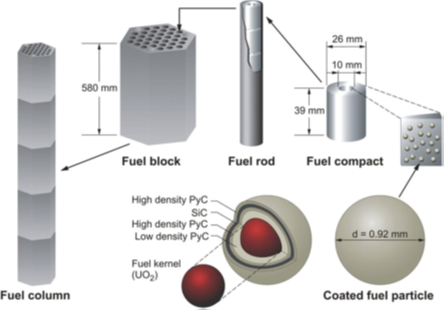
\includegraphics[width=0.6\textwidth]{figures/HTTR1.png}
        \caption{Fuel column loading of HTTR (obtained from \cite{bessEvaluationStartCore2009})}
        \label{fig:HTTR1}
\end{figure}

\begin{figure}[H]
        \centering
        \begin{subfigure}{.4\textwidth}
          \centering
          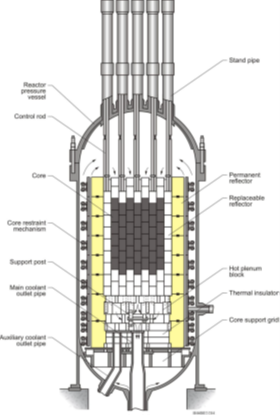
\includegraphics[width=\linewidth]{figures/HTTR2.png}
        \end{subfigure}
        \hfill
        \begin{subfigure}{.48\textwidth}
          \centering
          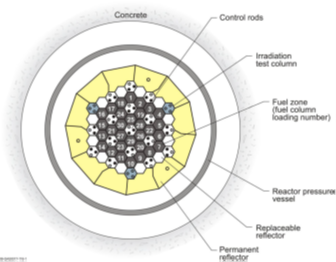
\includegraphics[width=\linewidth]{figures/HTTR3.png}
        \end{subfigure}
        \caption{Vertical (left) and horizontal (right) cross-sections of HTTR (obtained from \cite{bessEvaluationStartCore2009})}
        \label{fig:HTTR2}
\end{figure}

\begin{table}[H]
\centering
\caption{General parameters of HTTR}
\label{table:HTTRParam}

% Define custom color
\definecolor{myyellow}{RGB}{255, 255, 150}

\renewcommand{\arraystretch}{1.0} % row height

\begin{tabular}{|>{\raggedright\arraybackslash}p{8cm}|>{\centering\arraybackslash}m{3cm}|>{\centering\arraybackslash}m{3cm}|}
\hline
\rowcolor{myyellow}\multicolumn{3}{|c|}{\textbf{General Parameters}} \\ \hline
\centering\textbf{Parameter} & \textbf{Value} & \textbf{Unit} \\ \hline
Flat-to-flat core width & 436.48 & cm \\ \hline
Active core height (3D) & 522 & cm \\ \hline
Number of fuel block assembly & 30 & -- \\ \hline
Number of control block assembly & 19 & -- \\ \hline
Number of replaceable/permanent block assembly & 12/108 & -- \\ \hline

\rowcolor{myyellow}\multicolumn{3}{|c|}{\textbf{TRISO Kernels}} \\ \hline
Fuel kernel radius & 0.0300 & cm \\ \hline
Buffer layer outer radius & 0.0360 & cm \\ \hline
Inner PyC outer radius & 0.0390 & cm \\ \hline
SiC outer radius & 0.0415 & cm \\ \hline
Outer PyC radius & 0.0460 & cm \\ \hline
TRISO Packing Fraction & 30 & \% \\ \hline

\rowcolor{myyellow}\multicolumn{3}{|c|}{\textbf{Fuel Block Assembly}} \\ \hline
Fuel pin radius & 2.05 & cm \\ \hline
Coolant pin radius & 0.775 & cm \\ \hline
Burnable poison pin radius & 0.75 & cm \\ \hline
Number of fuel pins per block & 33 & -- \\ \hline
Number of burnable poison pins per block & 3 & -- \\ \hline
Fuel block height & 58 & cm \\ \hline
Flat-to-flat block width & 36 & cm \\ \hline
Fuel type & UO$_2$ & -- \\ \hline

\rowcolor{myyellow}\multicolumn{3}{|c|}{\textbf{Control Block Assembly}} \\ \hline
Control rod outer radius & 6.15 & cm \\ \hline
Control rod inner radius & 5.65 & cm \\ \hline

\rowcolor{myyellow}\multicolumn{3}{|c|}{\textbf{Coolant Block Assembly}} \\ \hline
Coolant pin radius & 1.15 & cm \\ \hline
Number of coolant pins per block & 33 & -- \\ \hline

\end{tabular}
\end{table}

For this dissertation, the design for HTTR startup core configuration with cold zero-power is used as the reference case. For the 2D case, not all variations of fuel enrichments are used. The 2D case is taken from the mid-plane block of the 3D case. The configuration map of the materials and fuel enrichment in the 2D case is shown in Figure \ref{fig:HTTR2Dconfig} \cite{bessEvaluationStartCore2009, zhangSimplifiedTwoThree2011}.

\begin{figure}[H]
        \centering
        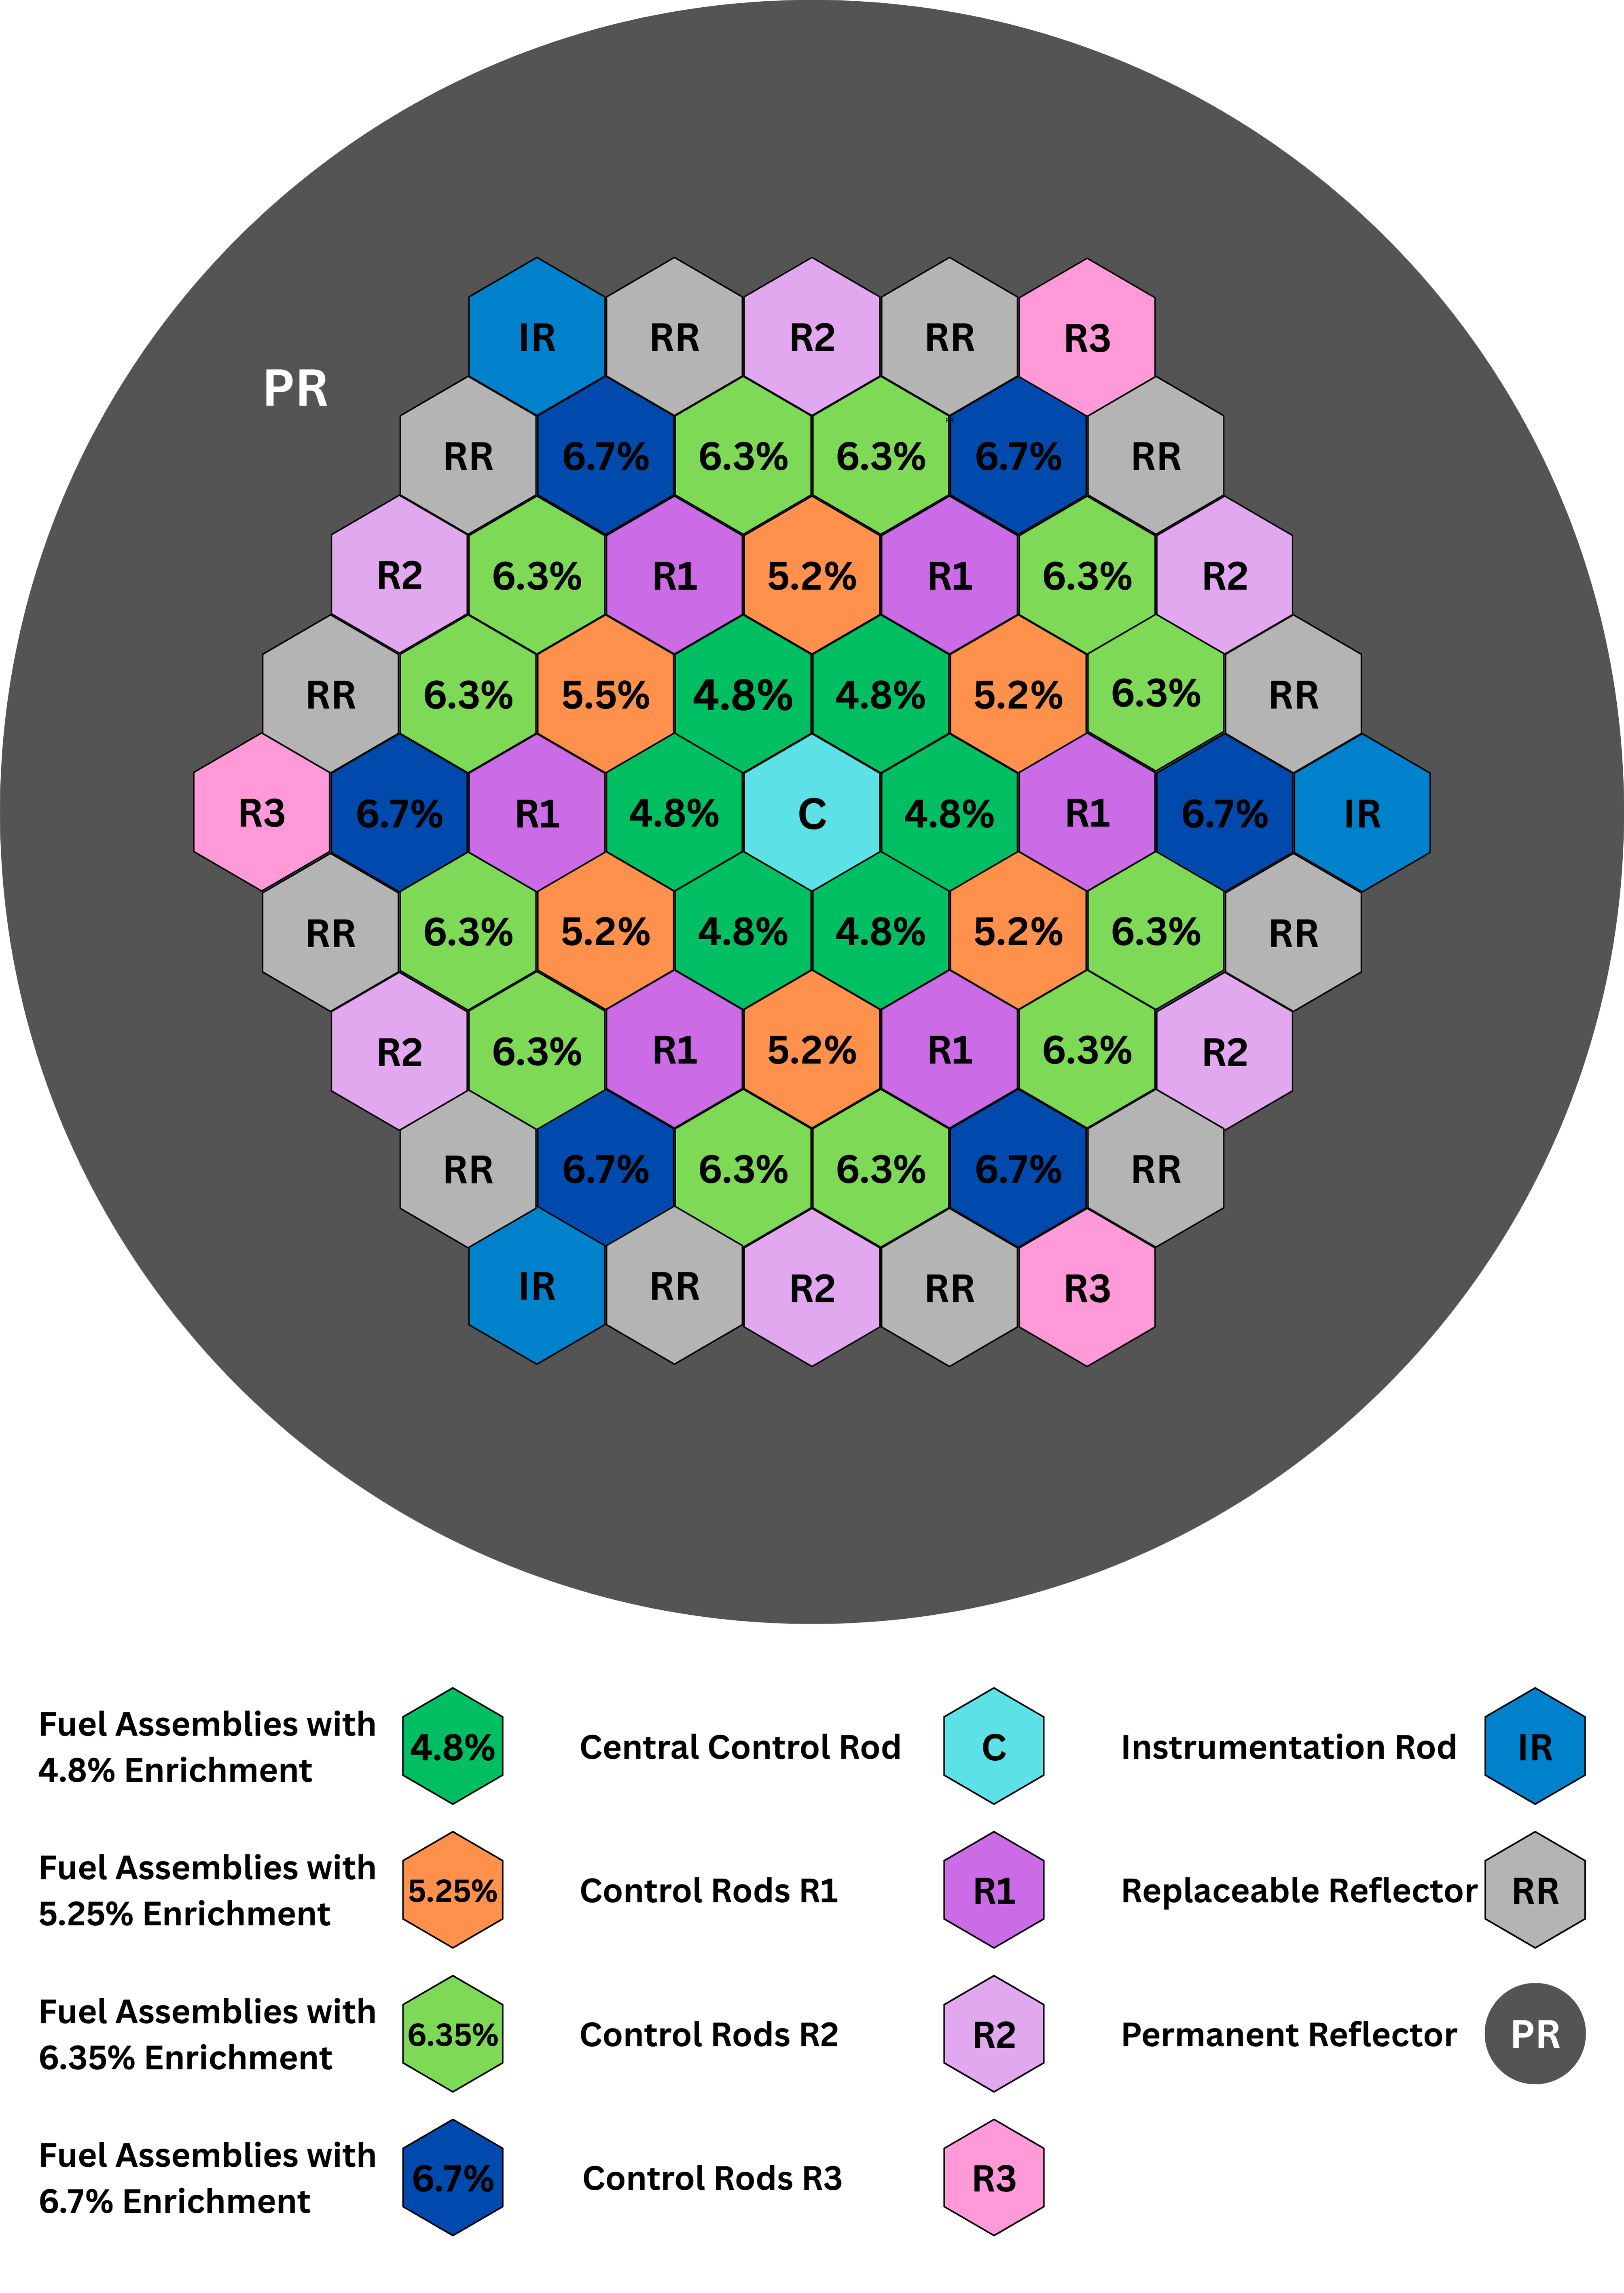
\includegraphics[width=0.45\textwidth]{figures/HTTR2Dconfig.png}
        \caption{Configuration map for 2D HTTR case}
        \label{fig:HTTR2Dconfig}
\end{figure}

For 3D case, the control rods are partially inserted to the level at which it is critical \cite{bessEvaluationStartCore2009, zhangSimplifiedTwoThree2011}. The configuration map of the 3D case in radial and axial directions is shown in Figure \ref{fig:HTTR3Dconfig} \cite{bessEvaluationStartCore2009, zhangSimplifiedTwoThree2011}.

\begin{figure}[H]
        \centering
        \begin{subfigure}{.48\textwidth}
          \centering
          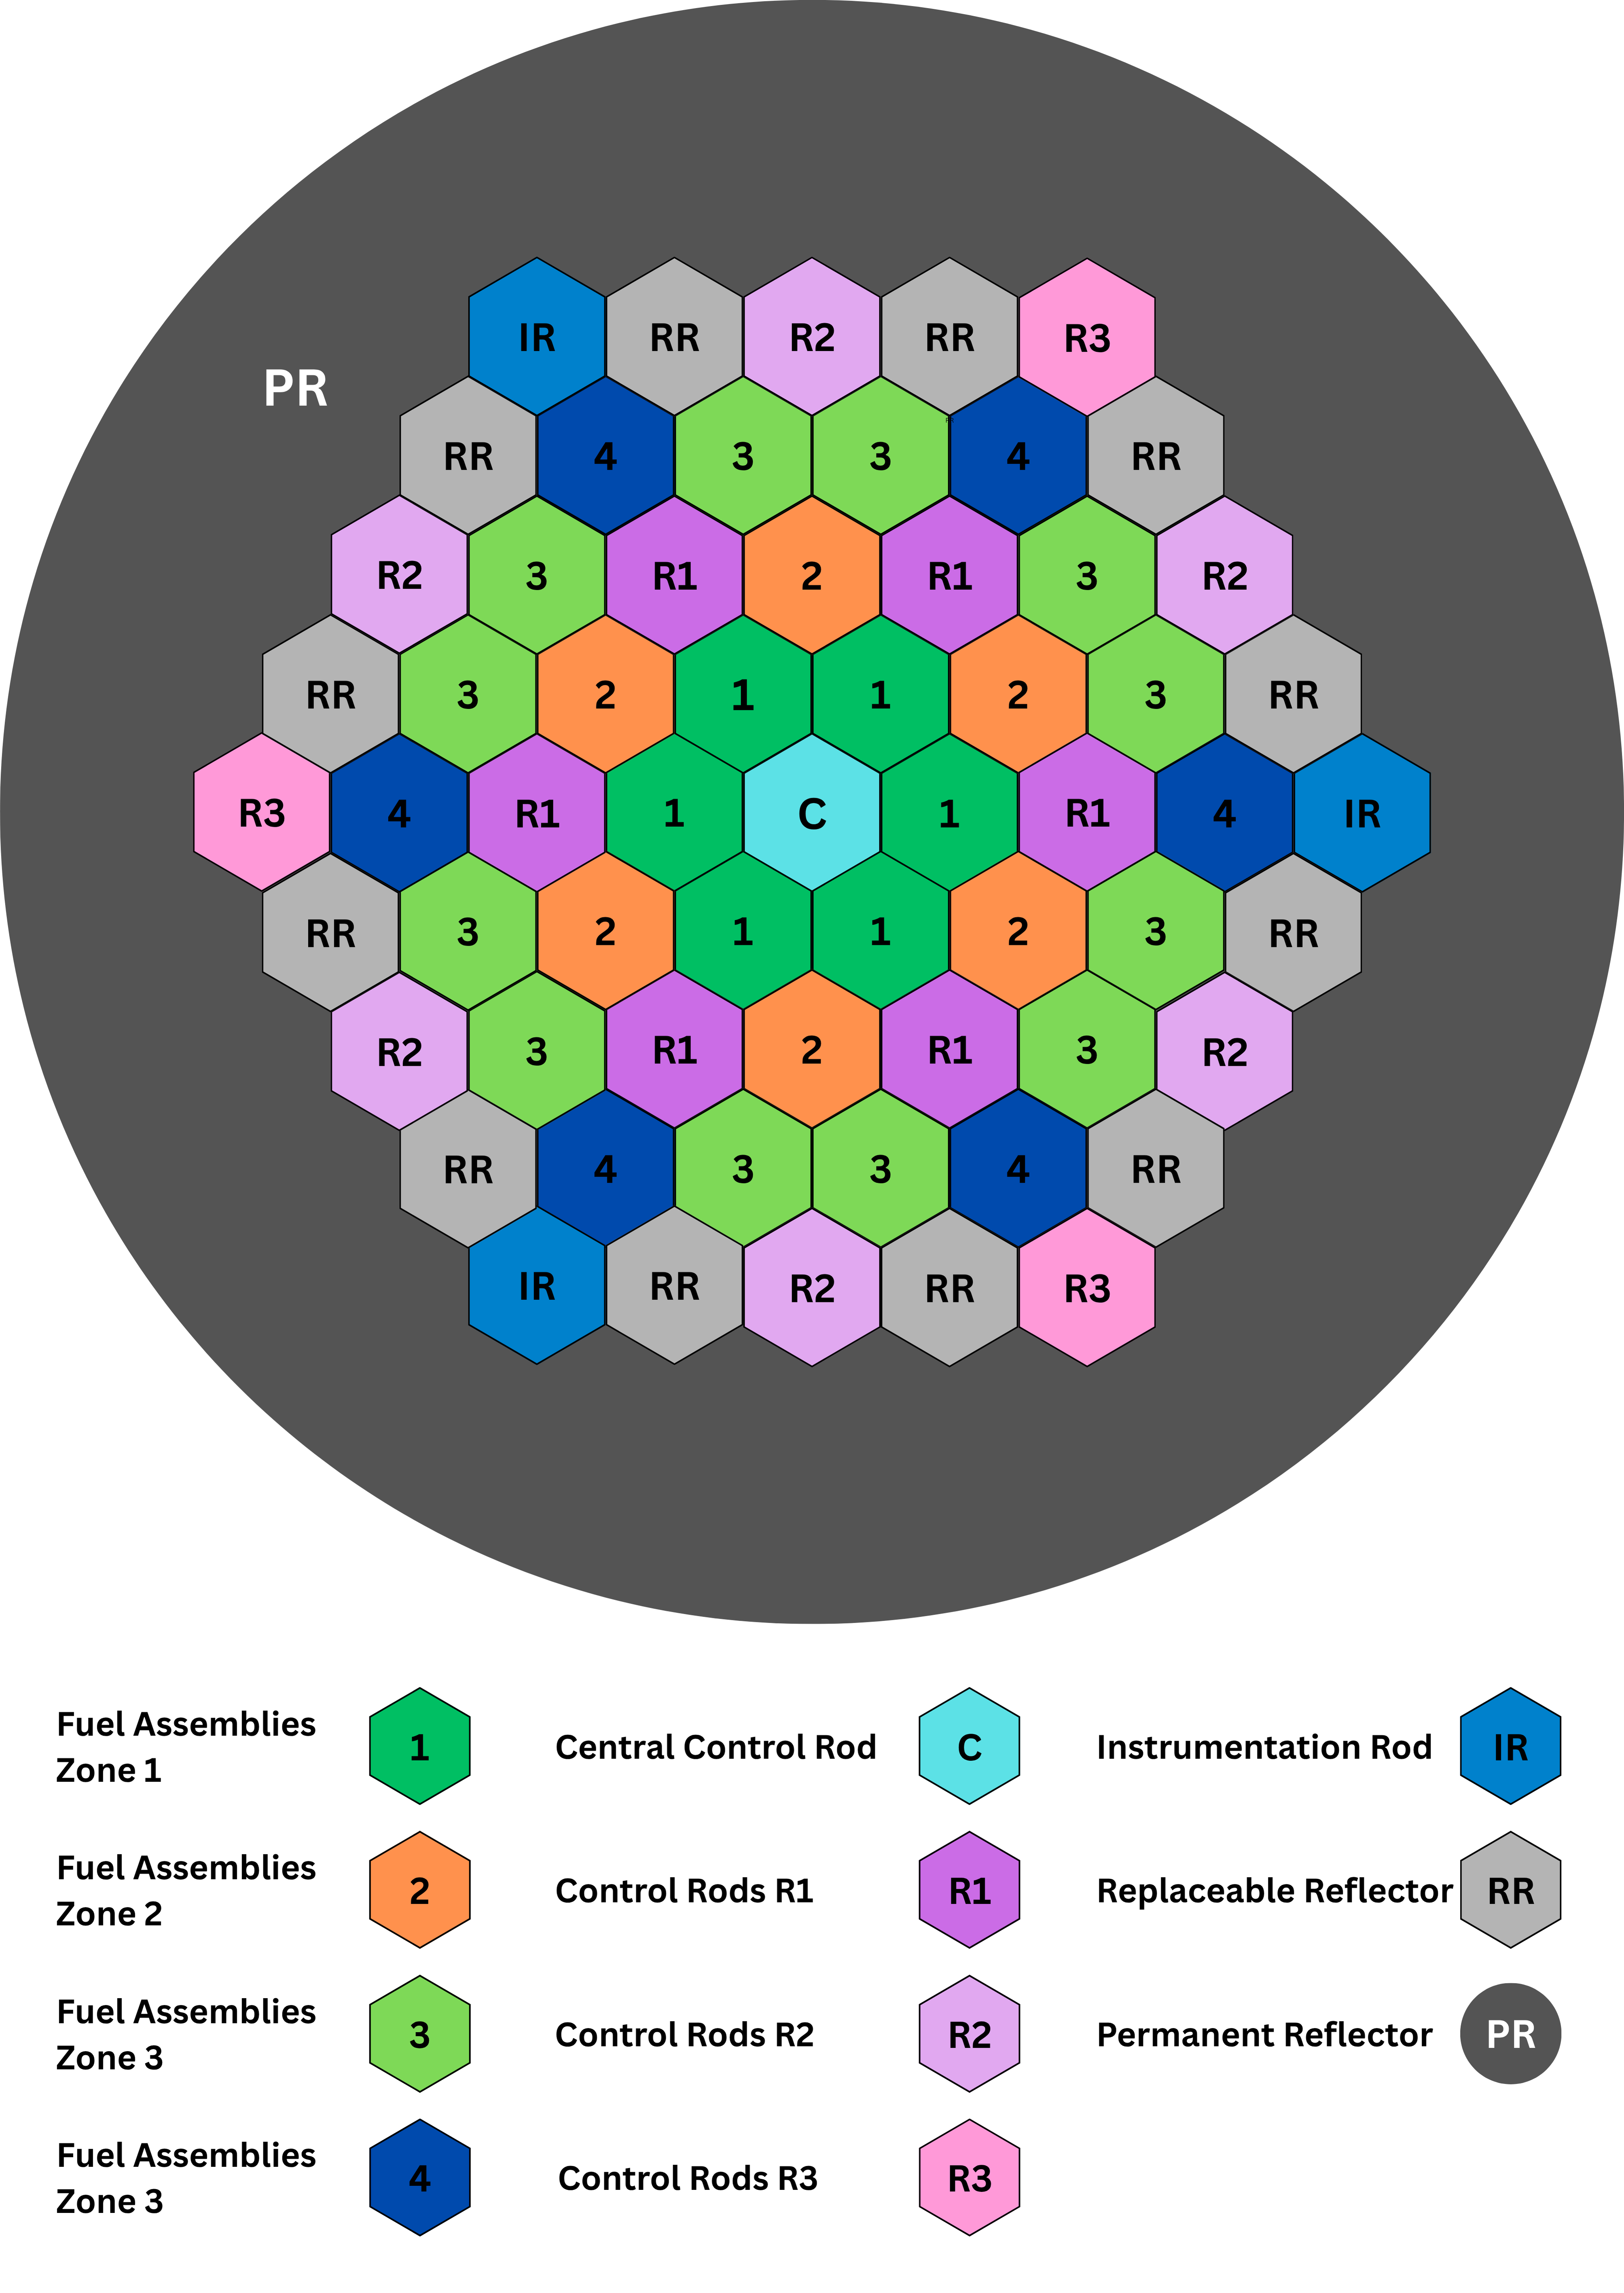
\includegraphics[width=\linewidth]{figures/HTTR3Dconfig1.png}
        \end{subfigure}
        \hfill
        \begin{subfigure}{.48\textwidth}
          \centering
          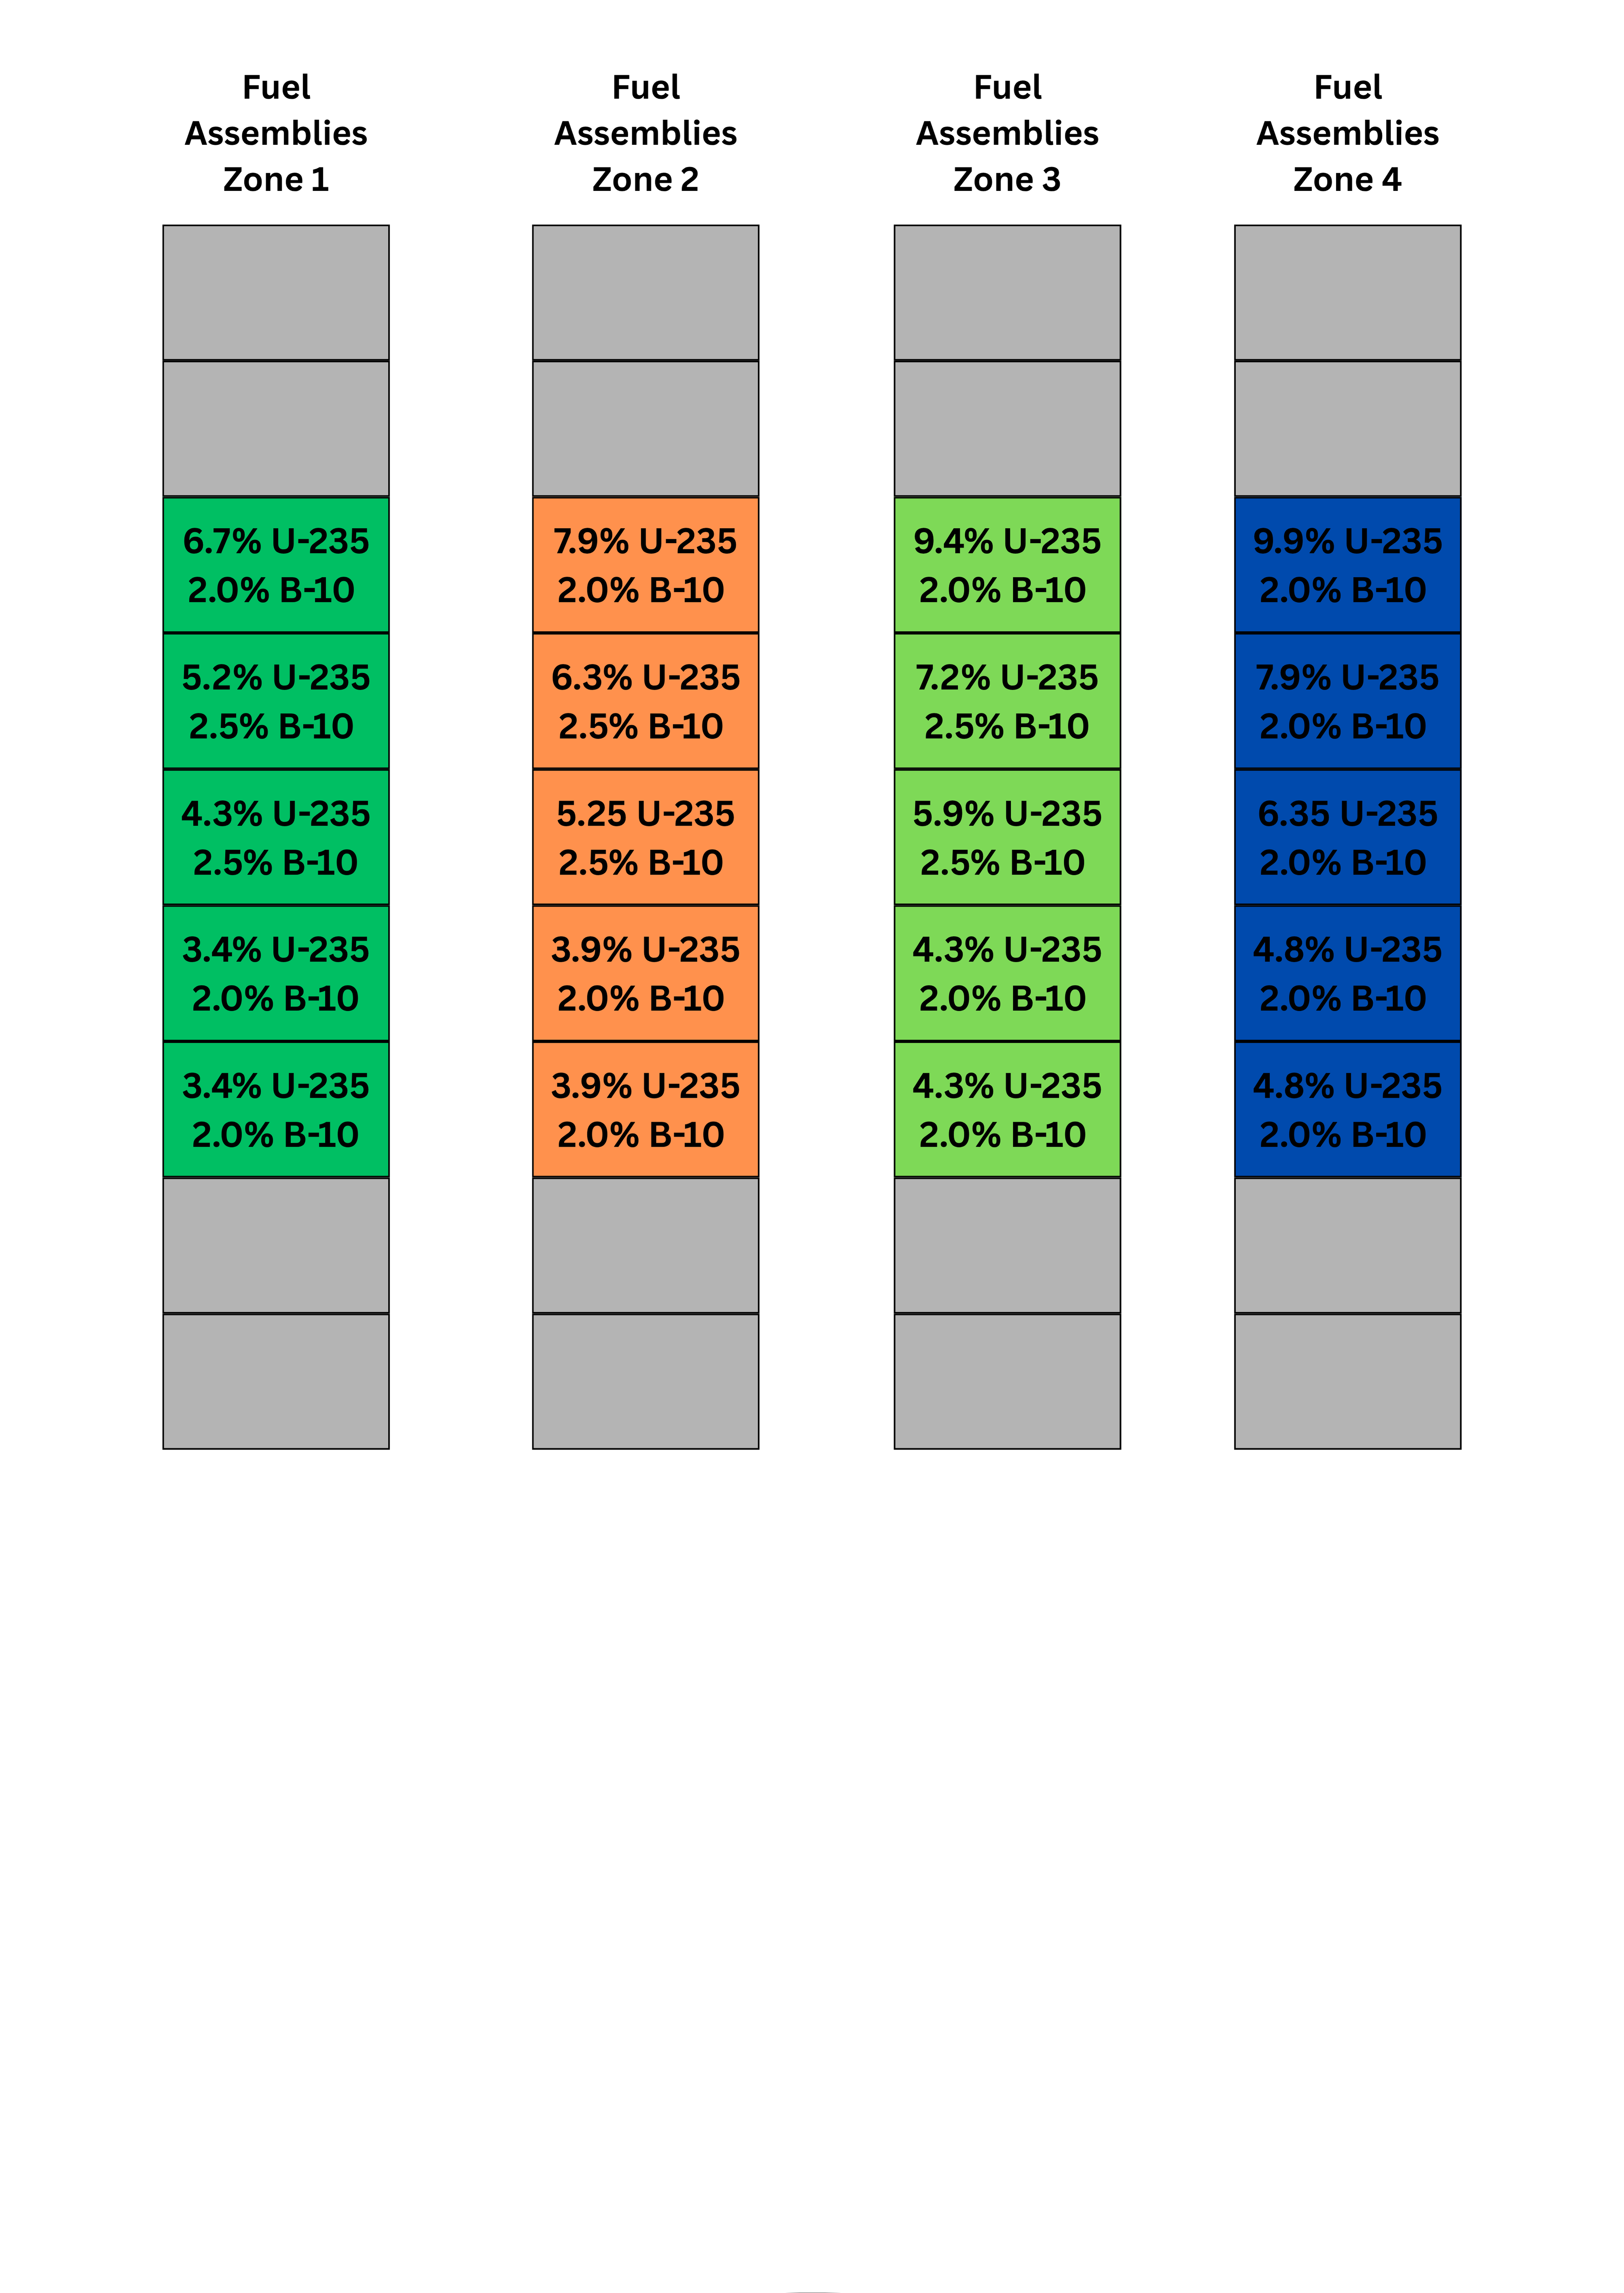
\includegraphics[width=\linewidth]{figures/HTTR3Dconfig2.png}
        \end{subfigure}
        \caption{Radial (left) and axial (right) configuration of 3D HTTR}
        \label{fig:HTTR3Dconfig}
\end{figure}

\section{Cross-section Homogenization using Serpent Monte Carlo Code}

The Serpent Monte Carlo code was developed by VTT Technical Research Center in Finland. It is a continuous-energy Monte Carlo particle code. Serpent has the capability to generate multigroup cross-sections for deterministic codes through spatial homogenization \cite{fridmanRevisedMethodsFewGroup2012, leppanenSerpentMonteCarlo2015}. Serpent has unique capabilities regarding the modeling of HTGRs. It has the capability to model the random TRISO distribution inside the fuel pellets. This modeling is done explicitly, in which the location of each TRISO fuel is generated using an automated disperser routine \cite{leppanenSerpentMonteCarlo2015}.

The spatial homogenization is used to preserve the local reaction balance when the group constants are generated from the solution of local heterogeneous transport. The homogenized, multigroup reaction cross-section $\Sigma_g$ is written as follows.
\begin{equation}
    \Sigma_g = \frac{\int_{E_g}^{E_{g-1}} dE \int_V dV \Sigma(\textbf{r}, E) \phi(\textbf{r}, E)}{\int_{E_g}^{E_{g-1}} dE \int_V dV \phi(\textbf{r}, E)}
\end{equation}
where $\phi(\textbf{r}, E)$ is the scalar flux. The integration is performed over the volume of the homogenized region and energy group. One of the advantages of using Monte Carlo simulations for cross-section homogenization is that the stochastic estimates of the integral values of the reaction rates and the integral value of the flux over space and energy can be obtained directly from the simulation \cite{leppanenOverviewMethodologySpatial2016}.

For this dissertation, homogenized cross-sections are generated for each block in the core, which is defined as a distinct universe. For the 2D core, 128 universes are defined, and for the 3D core, 1144 universes are defined. Each universe generates homogenized cross-sections that will be post-processed and used as inputs to the neutron noise simulation tool.

\section{Forward Simulation of HTTR}

\subsection{2D Forward Flux}

In this simulation, the solution for the developed tool is compared to the Serpent Monte Carlo results. The output of Serpent is assembly-averaged flux distribution, which is then normalized in the postprocess. For the developed tool, the output is the flux distribution for triangular mesh. In this case, each hexagon is divided into six triangles. To obtain the assembly-averaged flux distribution, we performed the following:
\begin{equation}
    \phi_{g,k} = \frac{\sum_{i=1}^I \phi_{g,i}}{V_k}
\end{equation}
where,
\begin{itemize}
    \item[] $\phi_{g,i}$ = Neutron flux for group $g$ and triangle $i$,
    \item[] $I$ = = Total number of triangles in every assembly, 
    \item[] $\phi_{g,k}$ = Neutron flux for group $g$ and assembly $k$, 
    \item[] $V_k$ = Volume of assembly $k$. 
\end{itemize}

The relative error is calculated as follows:
\begin{equation}\label{eq:error_serpent}
    \varepsilon_k = \frac{|\phi_{k,\text{calc}}-\phi_{k,\text{serpent}}|}{|\phi_{k,\text{serpent}}|}
\end{equation}
The results for these calculations are as follows:
\begin{table}[H]
        \centering
        \caption{Eigenvalue comparison of 2D HTTR}
        \label{table:2DHTTR_fw_results}
        \begin{tabular}{ | M{3.5cm} | M{4cm} | } 
         \hline
         $k_{\text{eff}}$ Serpent & 0.991938 $\pm$ 0.00012  \\
         \hline
         $k_{\text{eff}}$ Tool & 1.002590  \\
         \hline
         Absolute Error (pcm) & 1065.2  \\
         \hline
        \end{tabular}
\end{table}

\begin{figure}[H]
        \centering
        \begin{subfigure}{.48\textwidth}
          \centering
          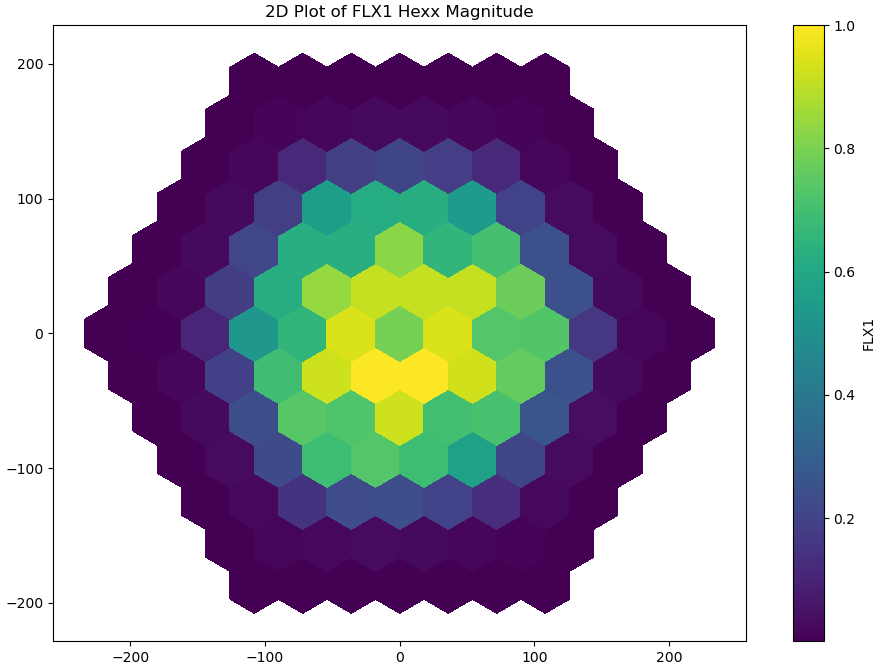
\includegraphics[width=\linewidth]{figures/OBJECTIVES1_TEST08_2DTriMG_HTTR2G_VandV_level1_FORWARD_FLX_magnitude_G1.png}
        \end{subfigure}
        \hfill
        \begin{subfigure}{.48\textwidth}
          \centering
          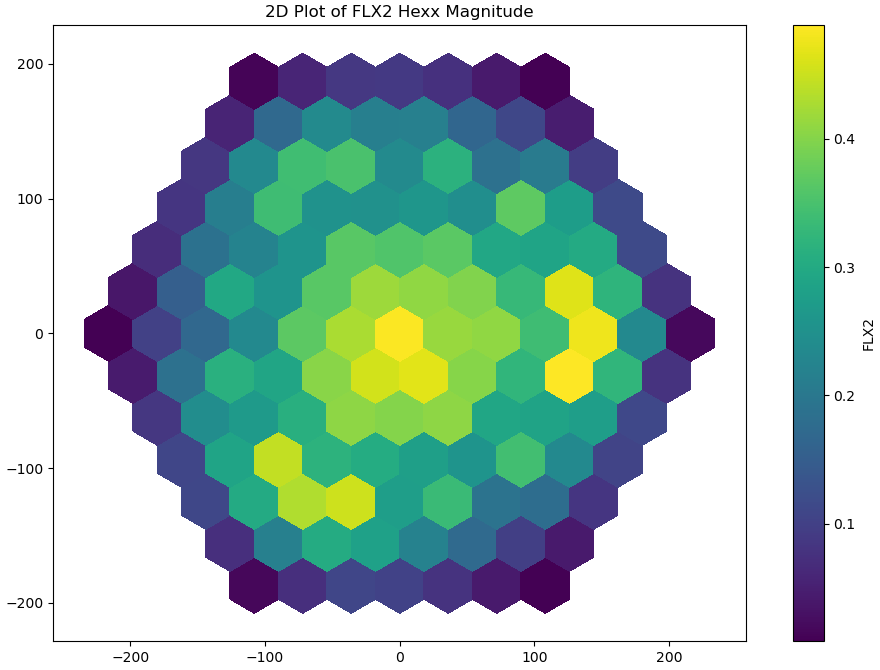
\includegraphics[width=\linewidth]{figures/OBJECTIVES1_TEST08_2DTriMG_HTTR2G_VandV_level1_FORWARD_FLX_magnitude_G2.png}
        \end{subfigure}
        \caption{Forward flux results from Serpent}
        \label{fig:2DHTTR_fw_results_flx}
\end{figure}
\begin{figure}[H]
        \centering
        \begin{subfigure}{.48\textwidth}
          \centering
          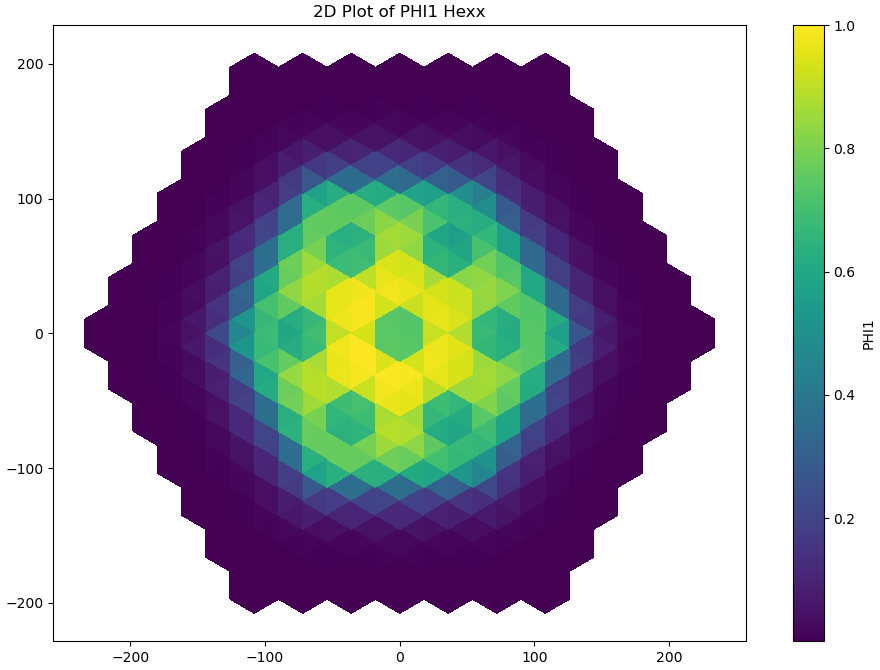
\includegraphics[width=\linewidth]{figures/OBJECTIVES1_TEST08_2DTriMG_HTTR2G_VandV_level1_FORWARD_PHI_magnitude_G1.png}
        \end{subfigure}
        \hfill
        \begin{subfigure}{.48\textwidth}
          \centering
          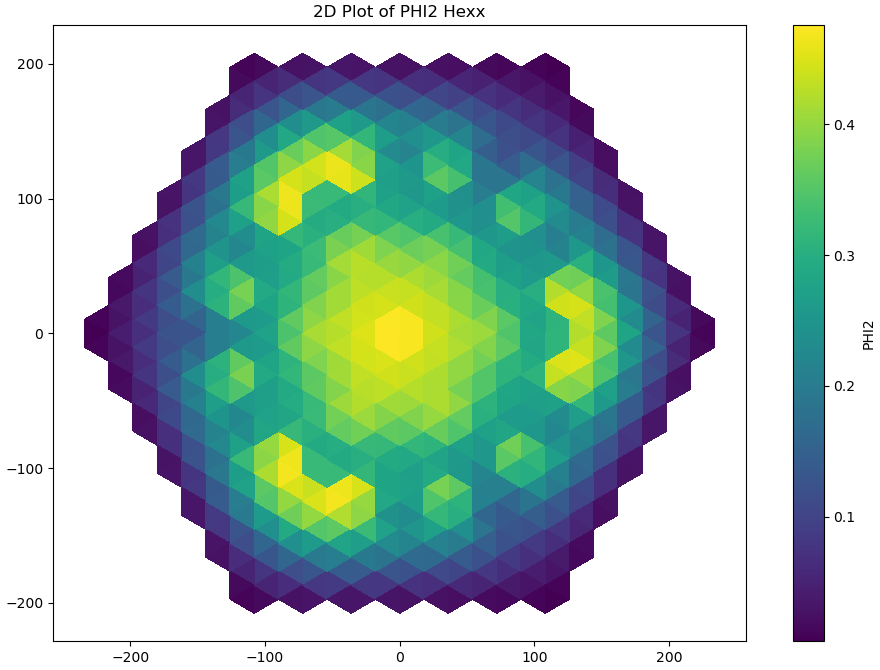
\includegraphics[width=\linewidth]{figures/OBJECTIVES1_TEST08_2DTriMG_HTTR2G_VandV_level1_FORWARD_PHI_magnitude_G2.png}
        \end{subfigure}
        \caption{Forward flux results from the developed tool}
        \label{fig:2DHTTR_fw_results_phi}
\end{figure}
\begin{figure}[H]
        \centering
        \begin{subfigure}{.48\textwidth}
          \centering
          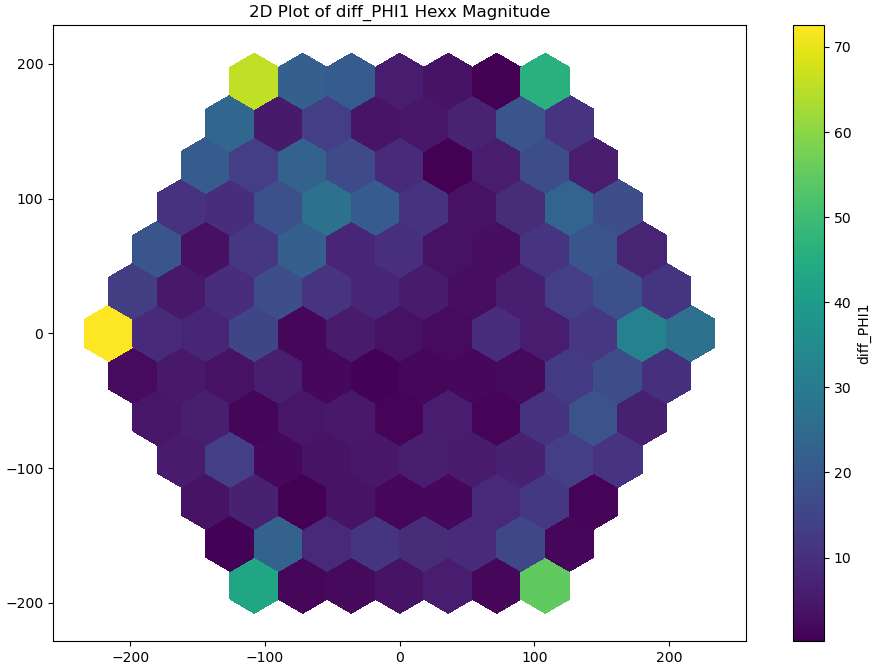
\includegraphics[width=\linewidth]{figures/OBJECTIVES1_TEST08_2DTriMG_HTTR2G_VandV_level1_FORWARD_diff_PHI_magnitude_G1.png}
        \end{subfigure}
        \hfill
        \begin{subfigure}{.48\textwidth}
          \centering
          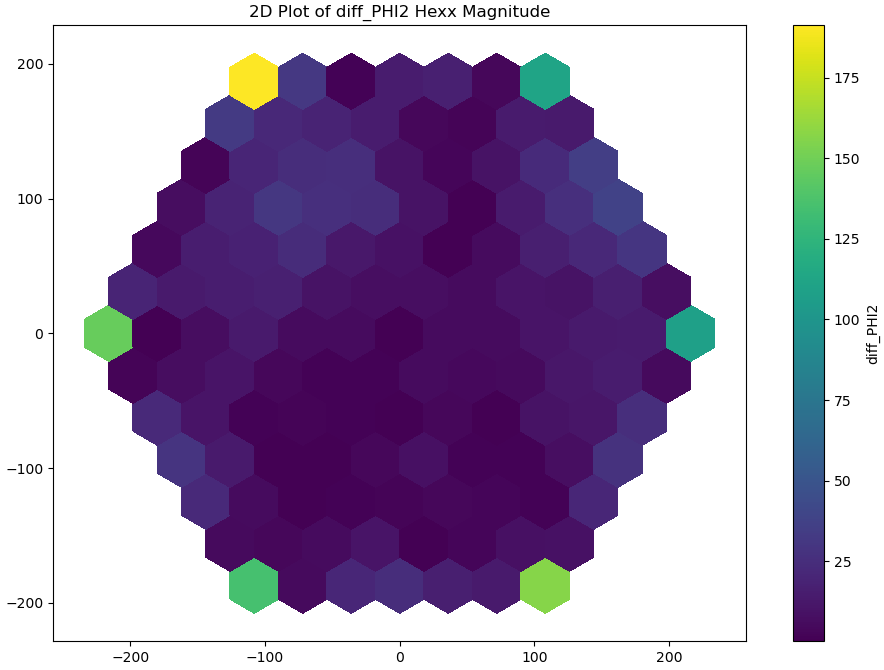
\includegraphics[width=\linewidth]{figures/OBJECTIVES1_TEST08_2DTriMG_HTTR2G_VandV_level1_FORWARD_diff_PHI_magnitude_G2.png}
        \end{subfigure}
        \caption{Difference of forward flux between Serpent and the tool}
        \label{fig:2DHTTR_fw_results_diff_phi}
\end{figure}

The results from Table \ref{table:2DHTTR_fw_results}, Figure \ref{fig:2DHTTR_fw_results_flx}, Figure \ref{fig:2DHTTR_fw_results_phi}, and Figure \ref{fig:2DHTTR_fw_results_diff_phi} show that, in general, the forward flux results obtained from the developed tool are in good agreement with the Serpent results. For the eigenvalue results, the difference in $k_{\text{eff}}$ is expected due to the homogenization of macroscopic cross-sections that are used in the developed tool. The heterogeneity effect of the HTTR is suppressed due to the spatial homogenization of the cross-sections. Also, the neutron diffusion method underestimates the neutron leakage due to its assumption of linear anisotropy. The flux differences are mainly in the periphery of the core. This behavior is expected, as the peripheral regions are filled with reflector materials, where the neutron flux is relatively low. 

\subsection{3D Forward Flux}

For the 3D forward flux simulation, the solution for the developed tool is compared to the Serpent Monte Carlo results. The output of Serpent is assembly-averaged flux distribution, which is then normalized in the postprocess. The assembly in this case is defined as a fuel block with a height of 58 cm. For the developed tool, the output is the flux distribution for each triangular prism. In this case, each hexagonal prism is divided into six triangular prisms. The error used in this case is defined in Eq. \ref{eq:error_serpent}. 

The results for these calculations are as follows:
\begin{table}[H]
        \centering
        \caption{Eigenvalue comparison of 3D HTTR}
        \label{table:3DHTTR_fw_results}
        \begin{tabular}{ | M{3.5cm} | M{4cm} | } 
         \hline
         $k_{\text{eff}}$ Serpent & 1.021540 $\pm$ 0.000094  \\
         \hline
         $k_{\text{eff}}$ Tool & 1.050390  \\
         \hline
         Absolute Error (pcm) & -2885.0  \\
         \hline
        \end{tabular}
\end{table}

\begin{figure}[H]
        \centering
        \begin{subfigure}{.48\textwidth}
          \centering
          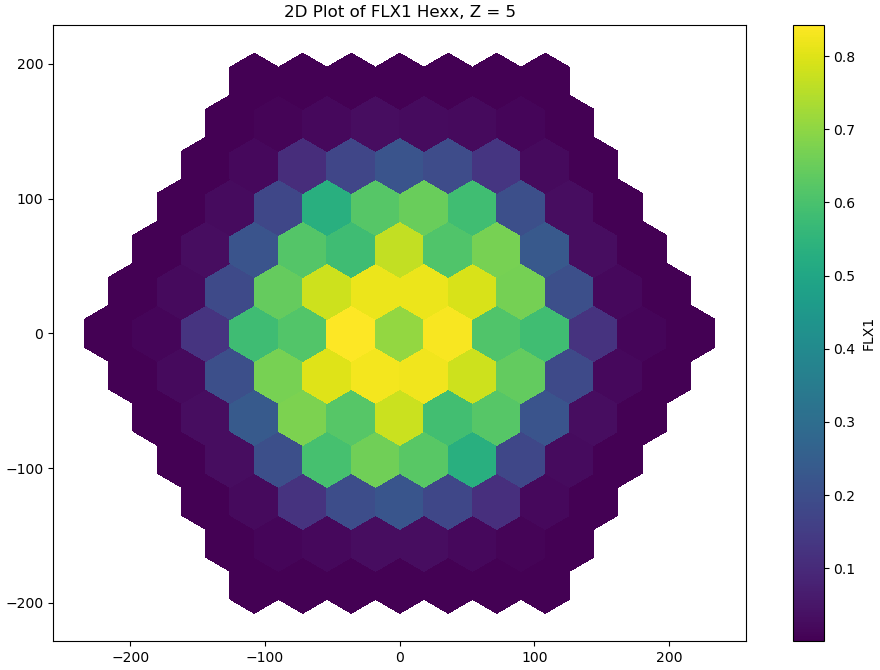
\includegraphics[width=\linewidth]{figures/OBJECTIVES1_TEST09_3DTriMG_HTTR_level1_FORWARD_FLX_magnitude_G1_Z5.png}
        \end{subfigure}
        \hfill
        \begin{subfigure}{.48\textwidth}
          \centering
          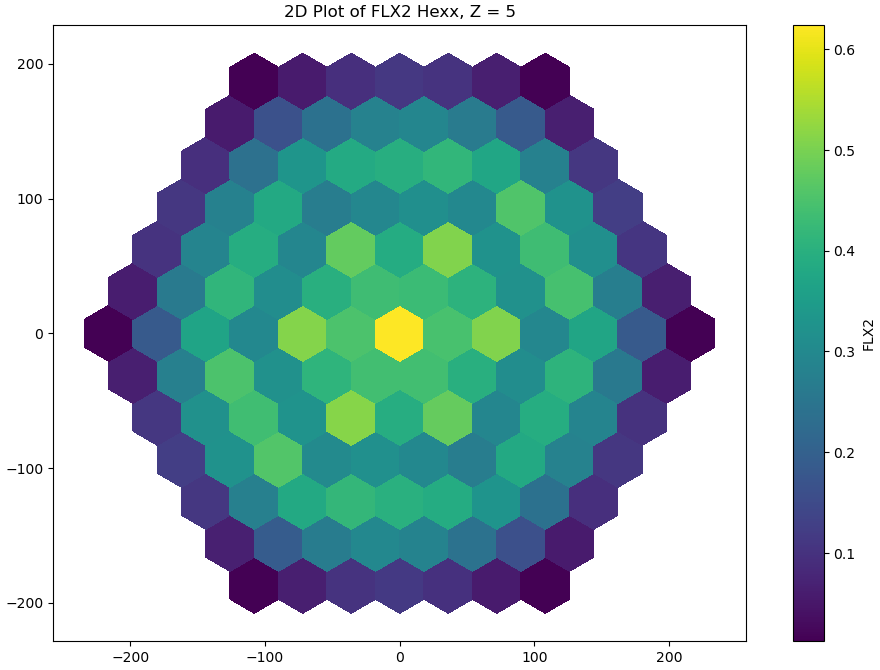
\includegraphics[width=\linewidth]{figures/OBJECTIVES1_TEST09_3DTriMG_HTTR_level1_FORWARD_FLX_magnitude_G2_Z5.png}
        \end{subfigure}
        \caption{Forward flux of 3D HTTR at midplane ($Z=5$) from Serpent}
        \label{fig:3DHTTR_fw_results_flx}
\end{figure}
\begin{figure}[H]
        \centering
        \begin{subfigure}{.48\textwidth}
          \centering
          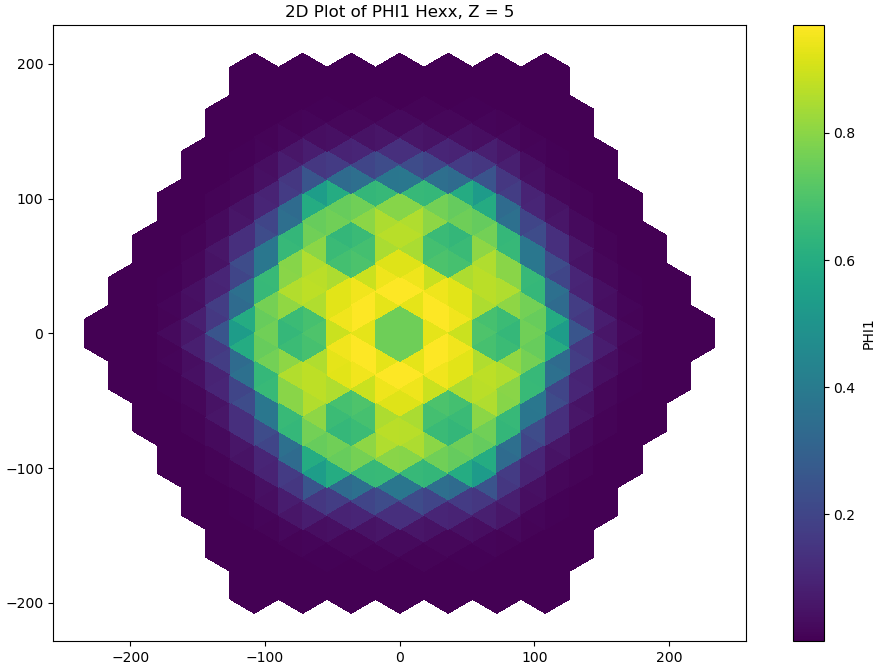
\includegraphics[width=\linewidth]{figures/OBJECTIVES1_TEST09_3DTriMG_HTTR_level1_FORWARD_PHI_magnitude_G1_Z5.png}
        \end{subfigure}
        \hfill
        \begin{subfigure}{.48\textwidth}
          \centering
          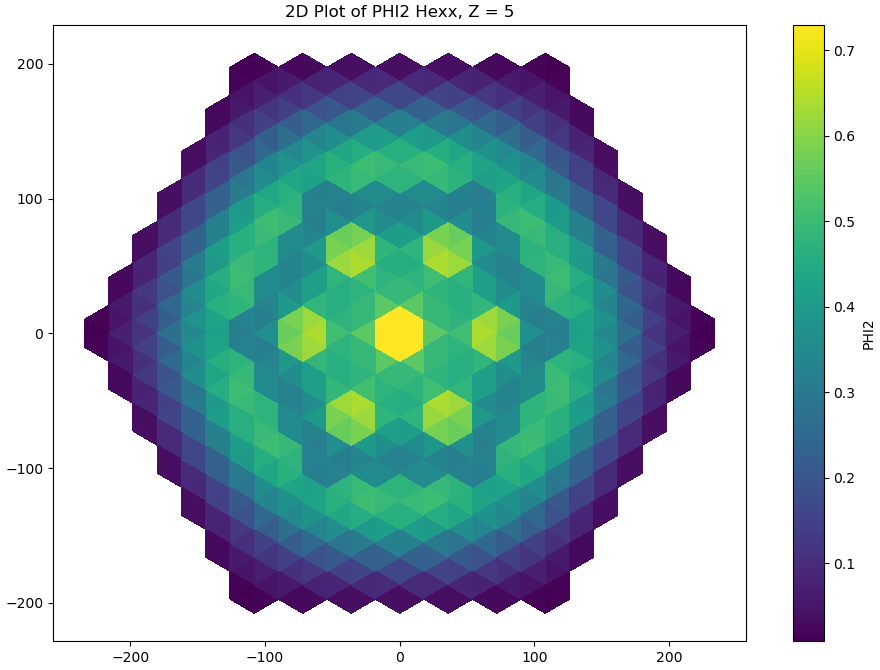
\includegraphics[width=\linewidth]{figures/OBJECTIVES1_TEST09_3DTriMG_HTTR_level1_FORWARD_PHI_magnitude_G2_Z5.png}
        \end{subfigure}
        \caption{Forward flux of 3D HTTR at midplane ($Z=5$) from the developed tool}
        \label{fig:3DHTTR_fw_results_phi}
\end{figure}
\begin{figure}[H]
        \centering
        \begin{subfigure}{.48\textwidth}
          \centering
          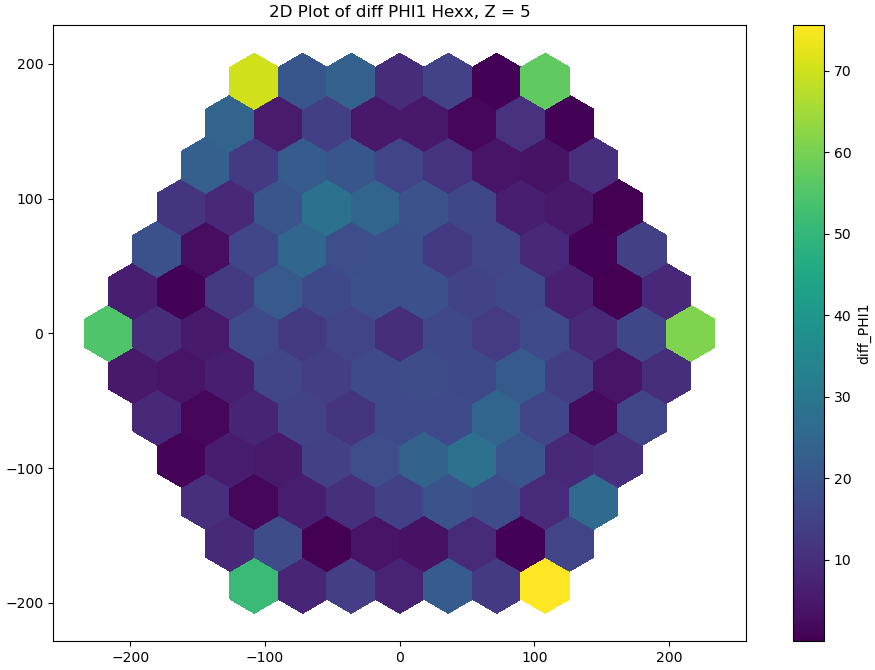
\includegraphics[width=\linewidth]{figures/OBJECTIVES1_TEST09_3DTriMG_HTTR_level1_FORWARD_diff_PHI_magnitude_G1_Z5.png}
        \end{subfigure}
        \hfill
        \begin{subfigure}{.48\textwidth}
          \centering
          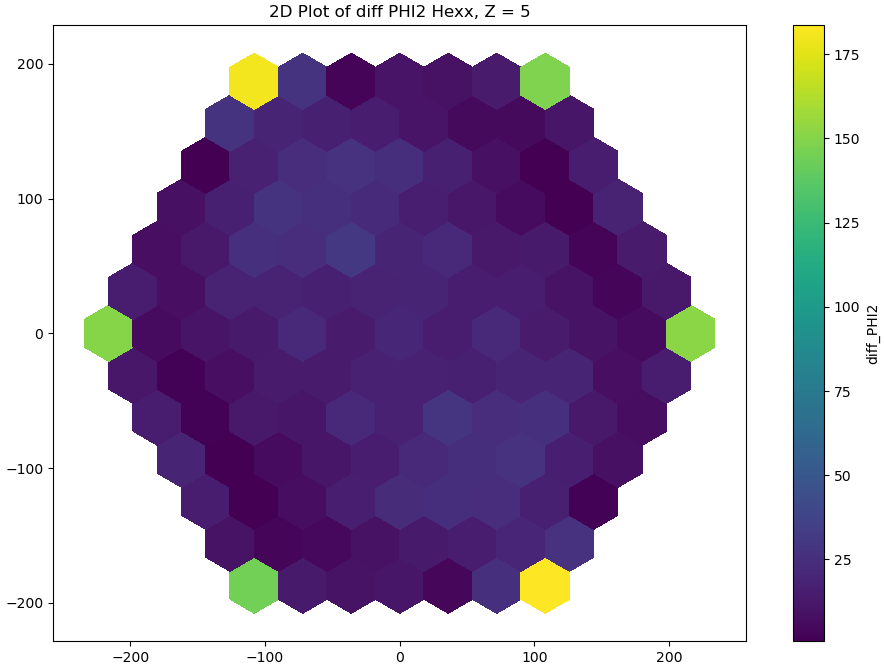
\includegraphics[width=\linewidth]{figures/OBJECTIVES1_TEST09_3DTriMG_HTTR_level1_FORWARD_diff_PHI_magnitude_G2_Z5.png}
        \end{subfigure}
        \caption{Difference of forward flux between Serpent and the developed tool}
        \label{fig:3DHTTR_fw_results_diff_phi}
\end{figure}

The results from Table \ref{table:3DHTTR_fw_results}, Figure \ref{fig:3DHTTR_fw_results_flx}, Figure \ref{fig:3DHTTR_fw_results_phi}, and Figure \ref{fig:3DHTTR_fw_results_diff_phi} show that, in general, the forward flux results obtained from the developed tool are in good agreement with the Serpent results. Overall, it shows similar observations compared to the 2D HTTR system. The difference in $k_{\text{eff}}$ is mainly due to the homogenization of macroscopic cross-sections and the assumption of neutron diffusion theory. The flux differences are primarily in the periphery of the core. This behavior is expected, as the peripheral regions are filled with reflector materials, where the neutron flux is relatively low. 

\section{Neutron Noise Simulation of HTTR}

\subsection{2D HTTR with Absorber of Variable Strength Source}

For this simulation, the neutron noise source is defined as a perturbation of the thermal absorption cross-section in the fuel assembly. The perturbation can be written as follows:
\begin{equation}
    \delta \Sigma_{a,2}(\textbf{r}, \omega) = \gamma(\omega) \delta(\textbf{r} - \textbf{r}_0)
\end{equation}
where $\gamma(\omega)$ is defined as 5\% of the thermal absorption cross-section at $r_0$ and $r_0$ is defined as one mesh in assembly number 65 (indicated as red triangle), which is shown in Figure \ref{fig:HTTR2DAVS}.
\begin{figure}[H]
        \centering
        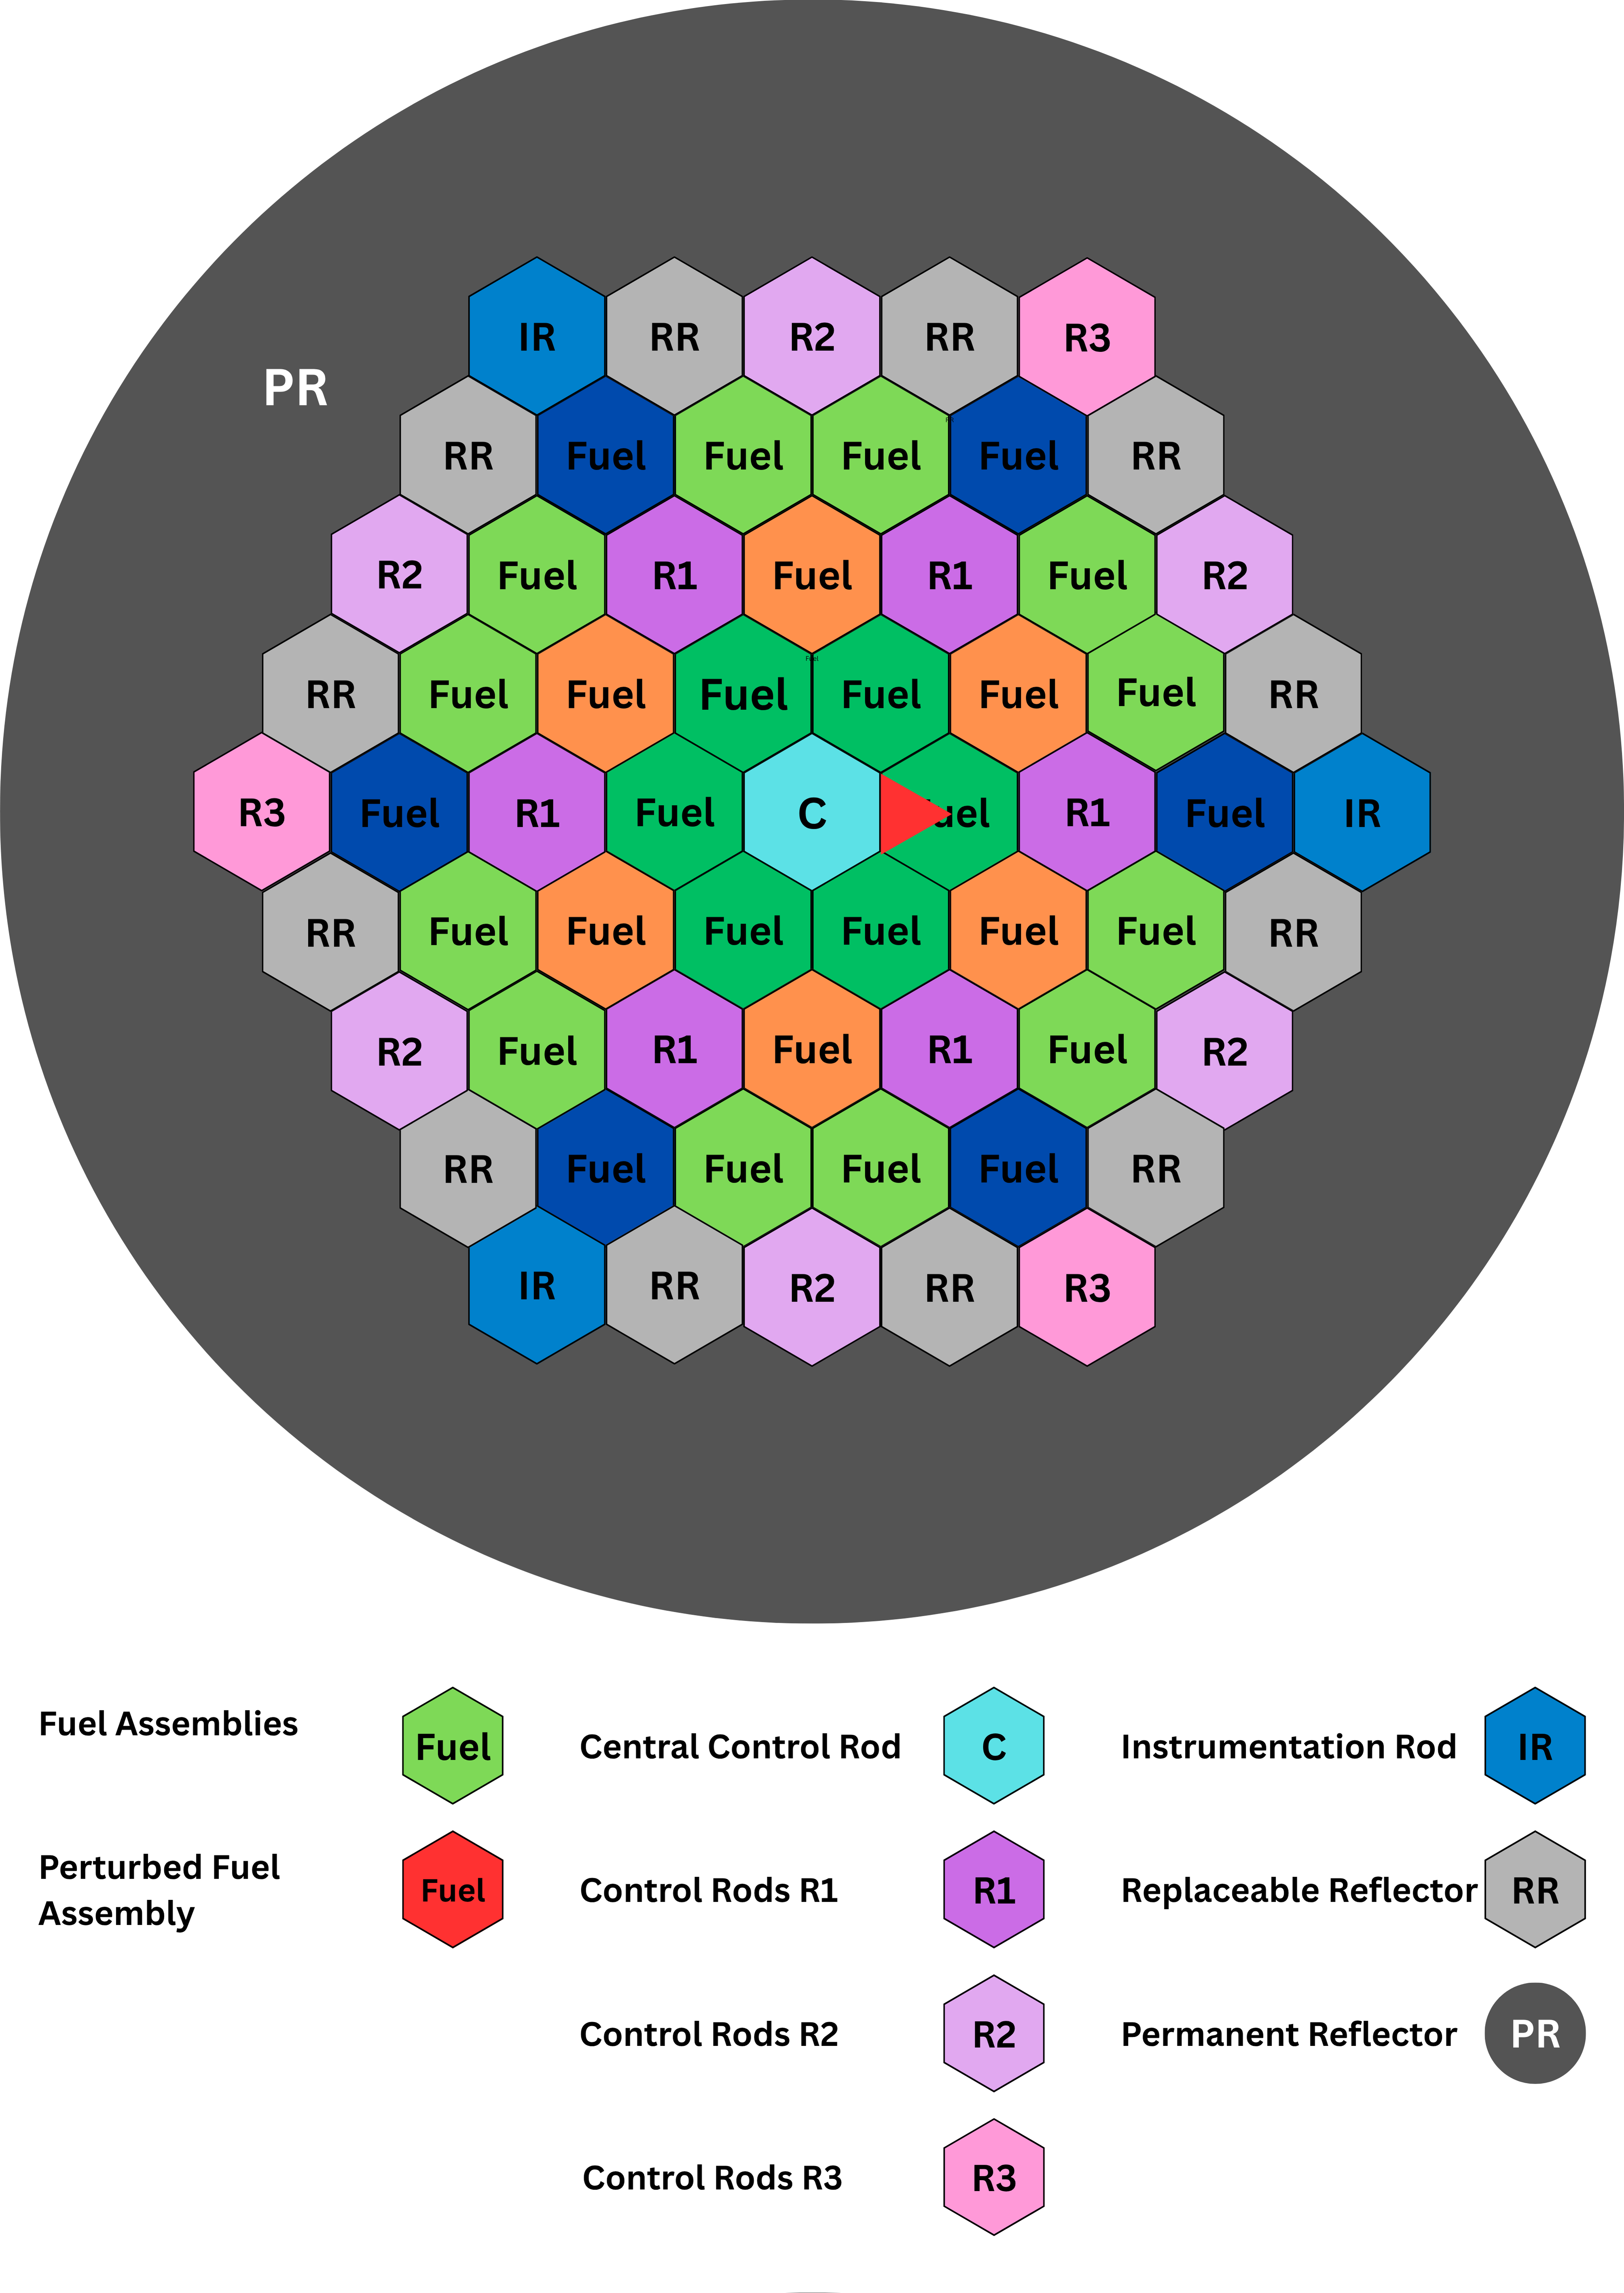
\includegraphics[width=0.45\textwidth]{figures/HTTR2DAVS.png}
        \caption{Location of the absorber of variable strength for 2D HTTR}
        \label{fig:HTTR2DAVS}
\end{figure}
The results of the simulations are as follows:
\begin{figure}[H]
        \centering
        \begin{subfigure}{.48\textwidth}
          \centering
          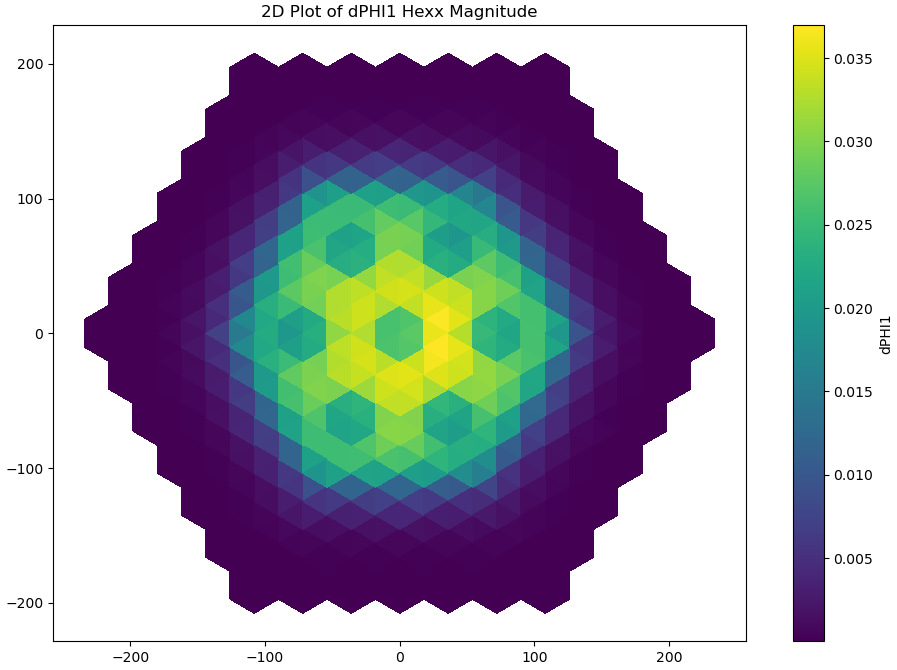
\includegraphics[width=\linewidth]{figures/OBJECTIVES3_TEST03_2DTriMG_HTTR2G_AVS_level1_NOISE_dPHI_magnitude_G1.png}
        \end{subfigure}
        \hfill
        \begin{subfigure}{.48\textwidth}
          \centering
          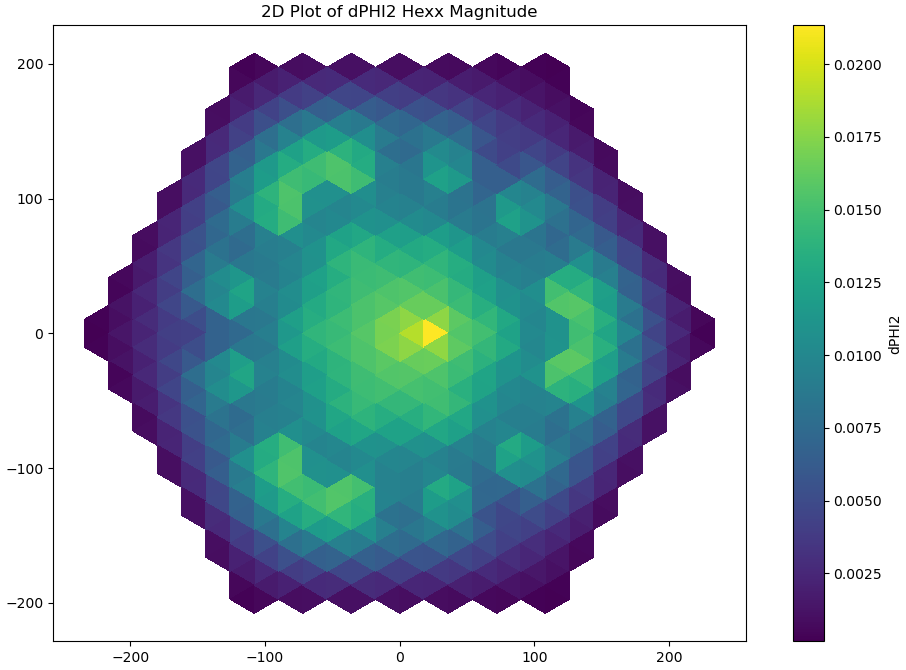
\includegraphics[width=\linewidth]{figures/OBJECTIVES3_TEST03_2DTriMG_HTTR2G_AVS_level1_NOISE_dPHI_magnitude_G2.png}
        \end{subfigure}
        \caption{Magnitude of the neutron noise for AVS in 2D HTTR}
        \label{fig:2DHTTR_noise_results_mag}
\end{figure}
\begin{figure}[H]
        \centering
        \begin{subfigure}{.48\textwidth}
          \centering
          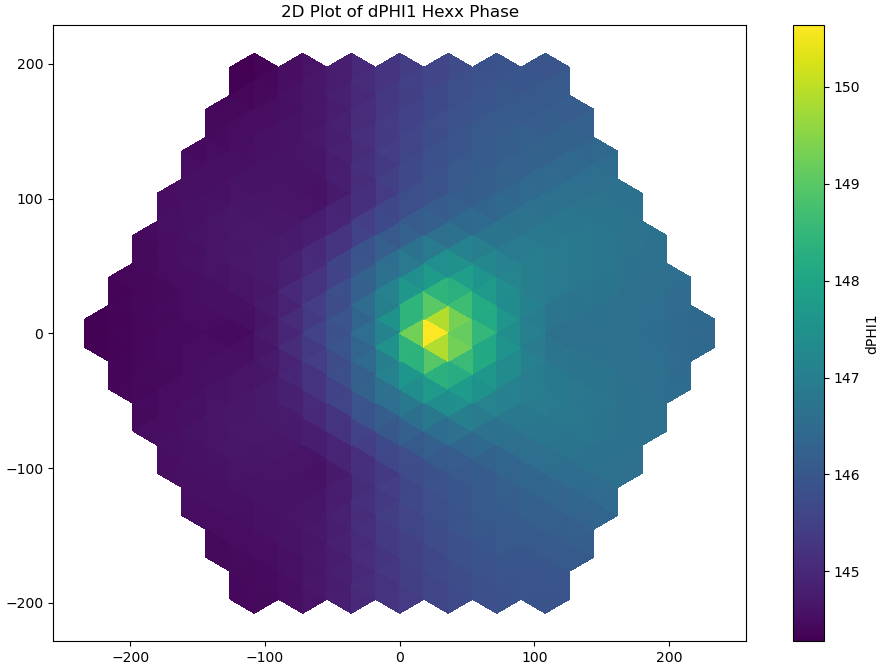
\includegraphics[width=\linewidth]{figures/OBJECTIVES3_TEST03_2DTriMG_HTTR2G_AVS_level1_NOISE_dPHI_phase_G1.png}
        \end{subfigure}
        \hfill
        \begin{subfigure}{.48\textwidth}
          \centering
          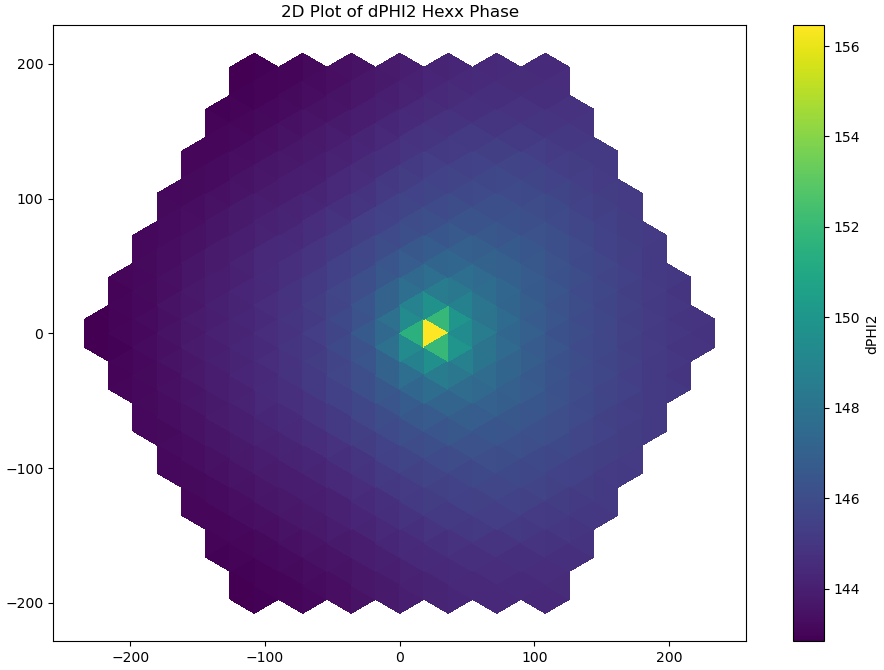
\includegraphics[width=\linewidth]{figures/OBJECTIVES3_TEST03_2DTriMG_HTTR2G_AVS_level1_NOISE_dPHI_phase_G2.png}
        \end{subfigure}
        \caption{Phase of the neutron noise for AVS in 2D HTTR}
        \label{fig:2DHTTR_noise_results_phase}
\end{figure}

Generally, the results indicate that the effect of neutron noise is more apparent in the thermal group. This is mainly due to the noise source located in the thermal spectrum only. We can also see in the phase delay plot (Figure \ref{fig:2DHTTR_noise_results_phase}) that the effect of neutron noise is more localized in the thermal group compared to the fast group. It should be noted that even though the neutron noise source is located at the thermal group only, the neutron noise in the fast group has a larger magnitude and is more dispersed compared to the thermal group. This is expected due to the larger mean free path of fast neutrons.

To further understand the driving force of neutron noise, we can split the neutron noise into its point kinetic component and its spatial component, as shown in Eq. \ref{eq:noise_component_time}. Figures \ref{fig:2DHTTRAVS_noise_component_results1} and \ref{fig:2DHTTRAVS_noise_component_results2} show the point kinetic component and spatial component of the neutron noise in fast and thermal group with AVS source, taken at the centerline of the core ($y=0$).
\begin{figure}[H]
        \centering
        \begin{subfigure}{.48\textwidth}
          \centering
          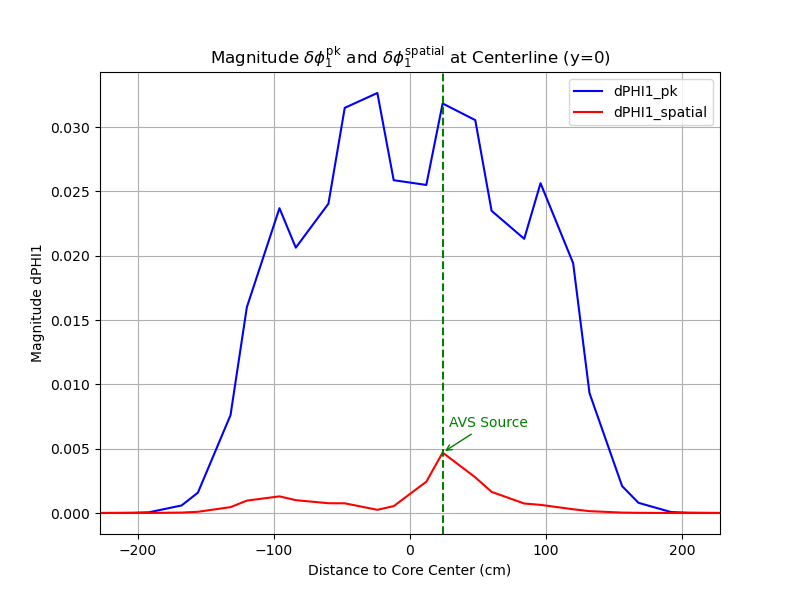
\includegraphics[width=\linewidth]{figures/Centerline_y0_OBJECTIVES3_TEST03_2DTriMG_HTTR2G_AVS_level1_dPHI_magnitude_G1.png}
        \end{subfigure}
        \hfill
        \begin{subfigure}{.48\textwidth}
          \centering
          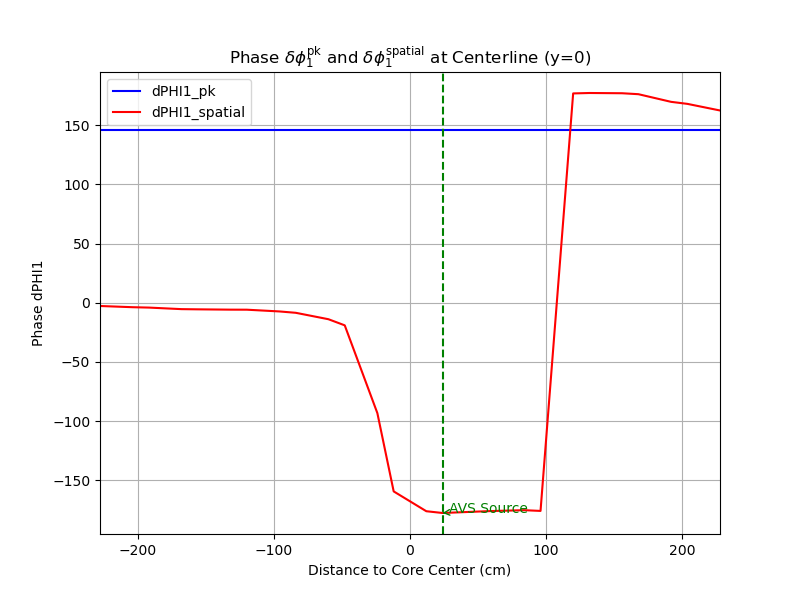
\includegraphics[width=\linewidth]{figures/Centerline_y0_OBJECTIVES3_TEST03_2DTriMG_HTTR2G_AVS_level1_dPHI_phase_G1.png}
        \end{subfigure}
        \caption{Magnitude (left) and phase (right) of the components of fast neutron noise for AVS in 2D HTTR, taken at centerline ($y=0$)}
        \label{fig:2DHTTRAVS_noise_component_results1}
\end{figure}
\begin{figure}[H]
        \centering
        \begin{subfigure}{.48\textwidth}
          \centering
          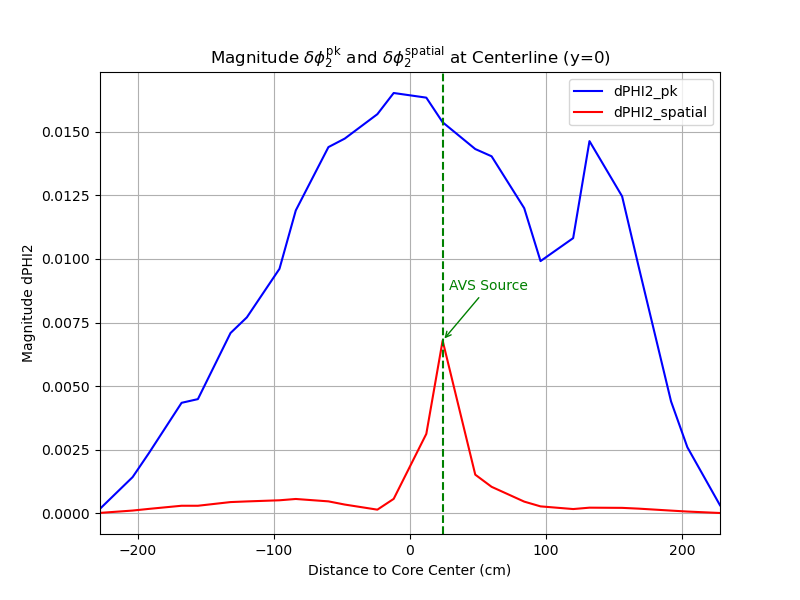
\includegraphics[width=\linewidth]{figures/Centerline_y0_OBJECTIVES3_TEST03_2DTriMG_HTTR2G_AVS_level1_dPHI_magnitude_G2.png}
        \end{subfigure}
        \hfill
        \begin{subfigure}{.48\textwidth}
          \centering
          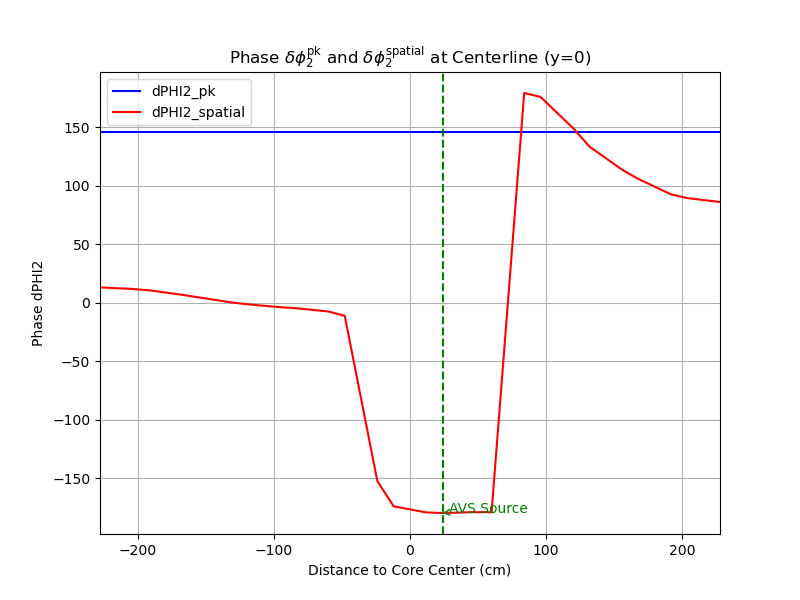
\includegraphics[width=\linewidth]{figures/Centerline_y0_OBJECTIVES3_TEST03_2DTriMG_HTTR2G_AVS_level1_dPHI_phase_G2.png}
        \end{subfigure}
        \caption{Magnitude (left) and phase (right) of the components of thermal neutron noise for AVS in 2D HTTR, taken at centerline ($y=0$)}
        \label{fig:2DHTTRAVS_noise_component_results2}
\end{figure}
Comparing Figure \ref{fig:2DHTTRAVS_noise_component_results1} and Figure \ref{fig:2DHTTRAVS_noise_component_results2}, we can see that in the fast group, the magnitude of the point kinetic component is has higher magnitude compared to the spatial component. This makes the magnitude of the neutron noise in the fast group more dispersed, following the point kinetic component. In the thermal group, the point kinetic component is also higher compared to the spatial component, but not at the same ratio as the fast group. This makes the contribution of the spatial component more apparent in the thermal group. The variation of the phase delay is mainly driven by the spatial components. This means that the phase of the spatial component drives the out-of-phase behavior of the neutron noise in the system. It is expected that the point kinetic component will have no effect on the phase delays since it is a factor of the forward flux. Overall, we can see that the point kinetic component is more dominant in 2D HTTR, which means that the neutron noise is driven by the reactivity effect of the perturbation.

\subsection{2D HTTR with Fuel Assembly Vibration Source}

For the simulation of the fuel assembly vibration, the neutron noise source is modeled using the $\varepsilon/d$ method. This means perturbation is a time-dependent sinusoidal function with amplitude $\varepsilon$ and frequency $\omega_0$. In this case, the frequency of vibration ($\omega_0$) is defined as 1 Hz, and the amplitude of vibration ($\varepsilon$) is 0.5 cm. Using this definition, the neutron noise source model is written as follows:
\begin{equation}
    \delta \Sigma_{a,g} (\textbf{r}_b,\omega) = \left\{
\begin{array}{ll}
      -i \pi \varepsilon \Delta  \Sigma_{a,g} \delta (\omega - \omega_0) & \textbf{r}_b-\varepsilon\leq y \leq \textbf{r}_b + \varepsilon \\
      0 & \text{otherwise}\\
\end{array} 
\right. 
\end{equation}
This means that all the interfaces of the assembly become the source of neutron noise. This differs from rectangular geometry cases, where the vibration can be defined in one axis and the other axis remains constant. The vibration is located at assembly number 65, as shown in Figure \ref{fig:HTTR2DFAV}.
\begin{figure}[H]
        \centering
        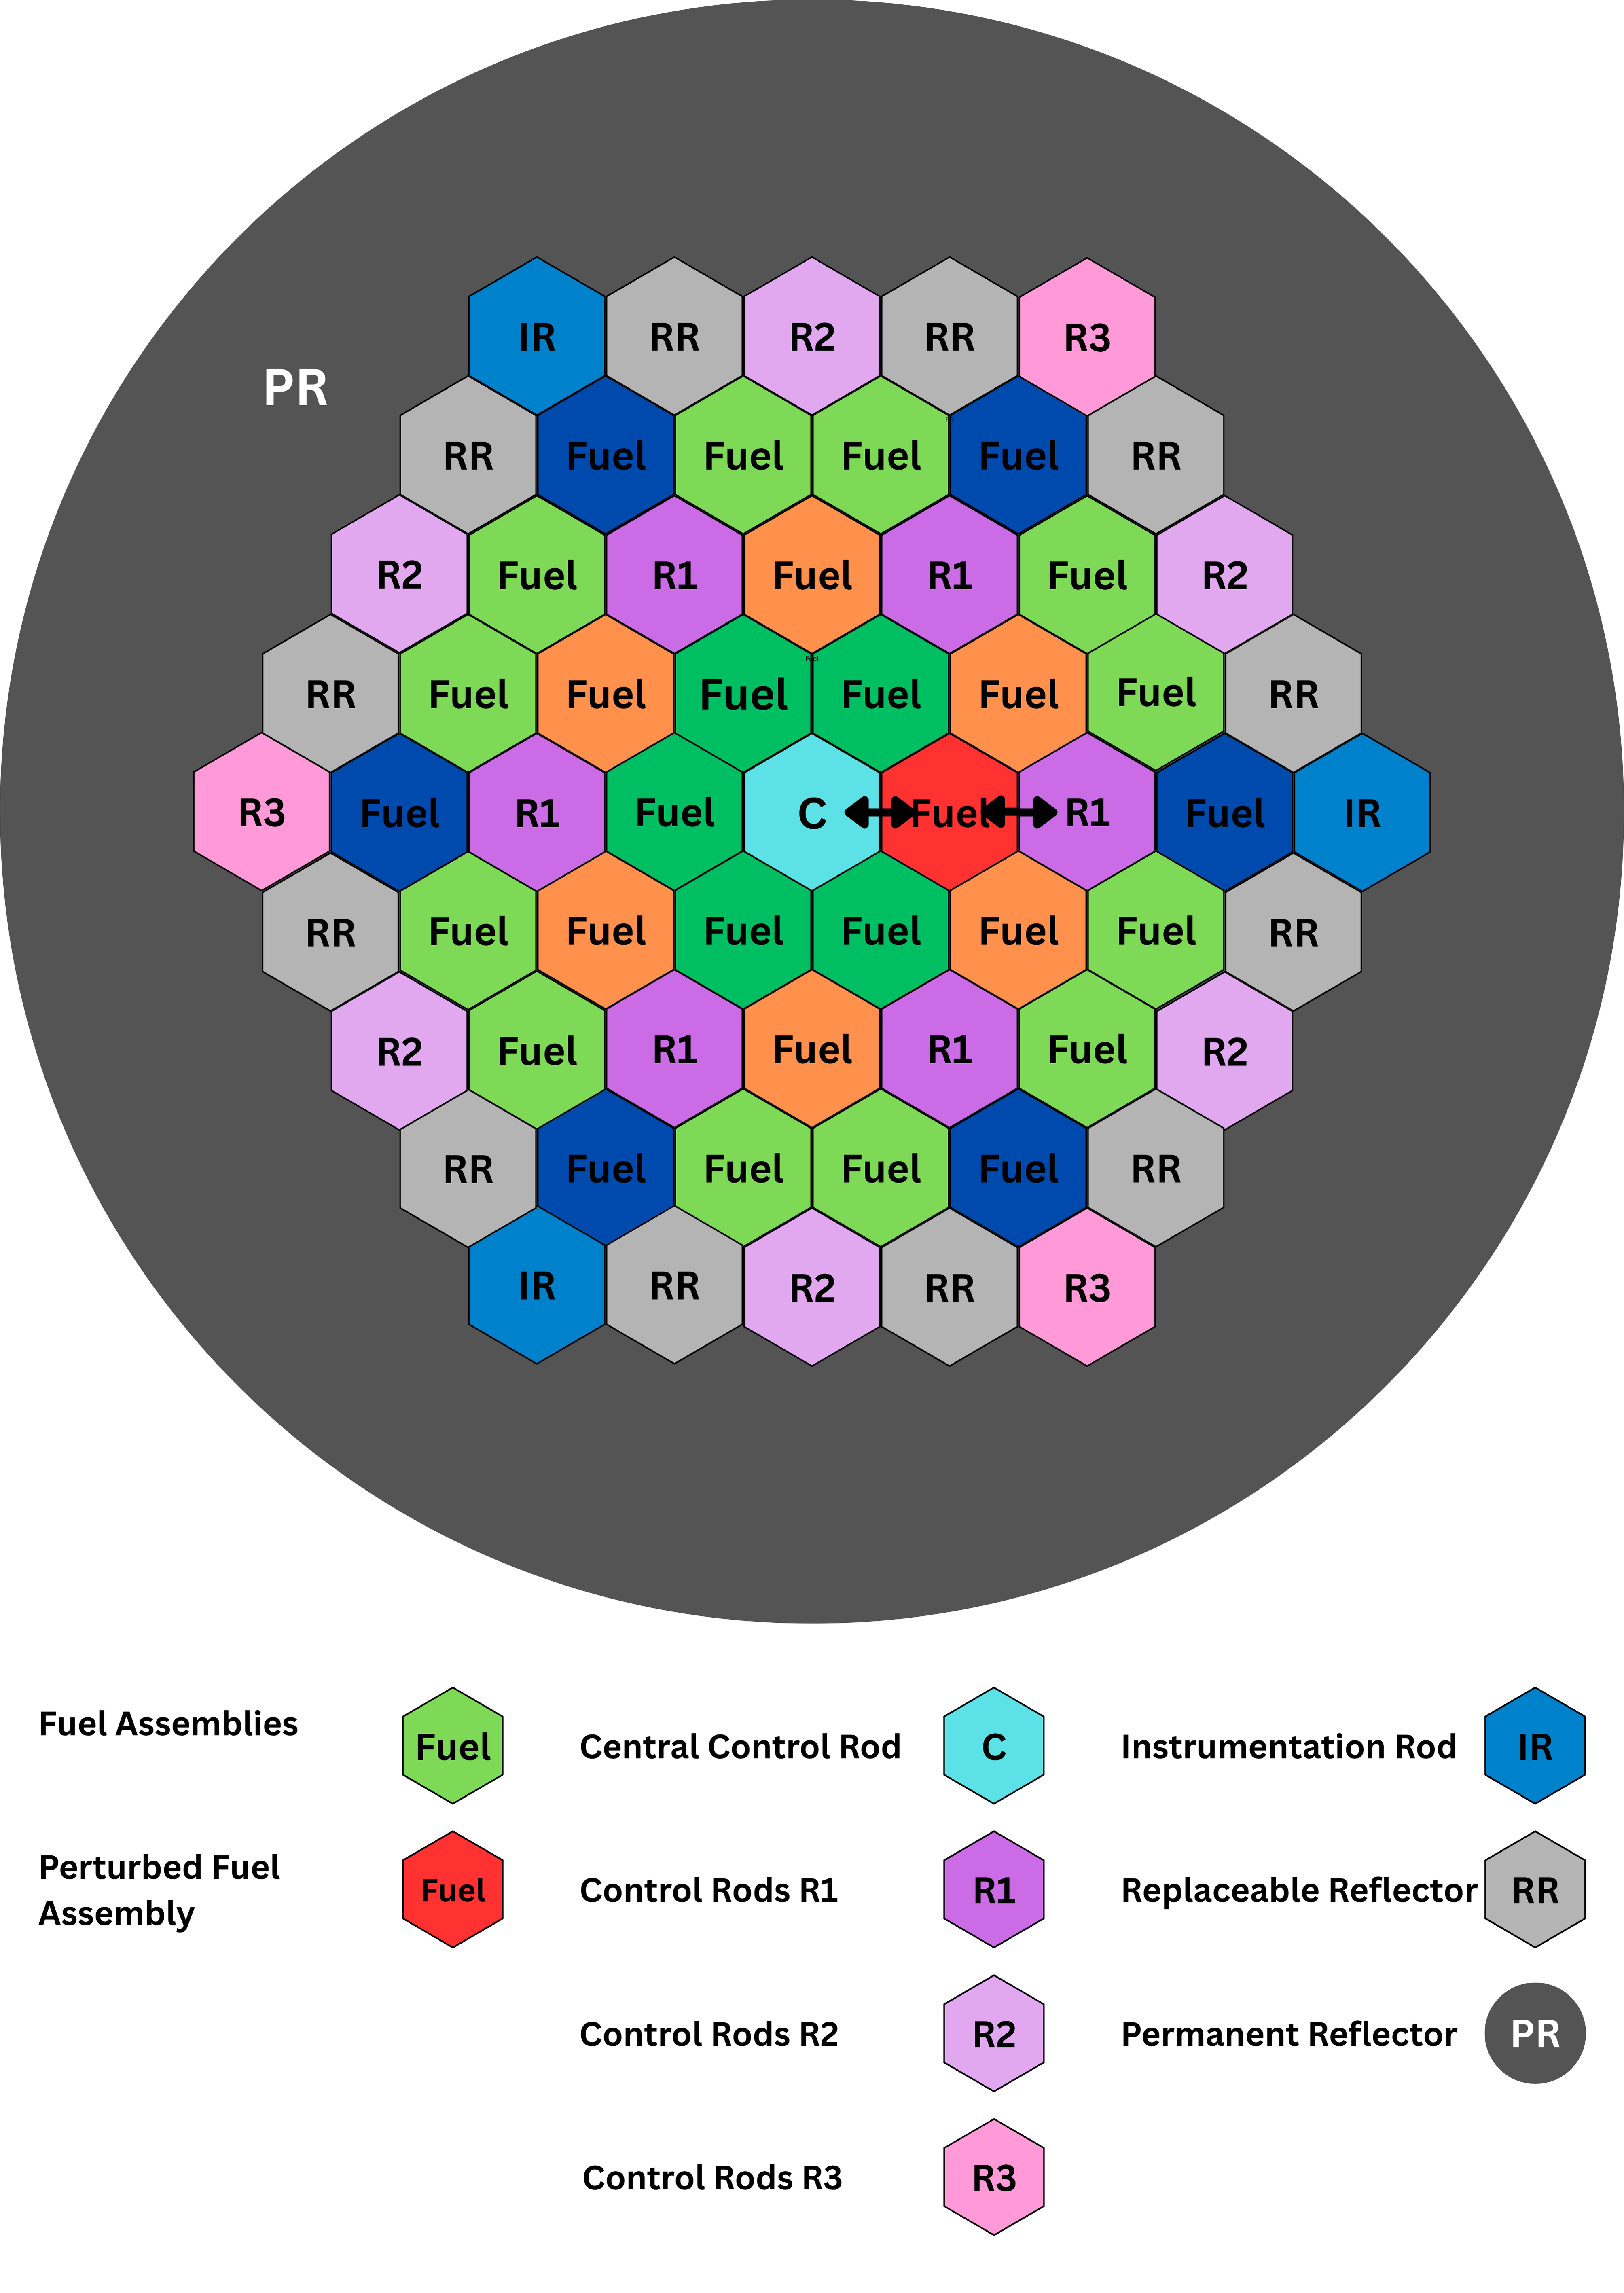
\includegraphics[width=0.45\textwidth]{figures/HTTR2DFAV.png}
        \caption{Location of the fuel assembly vibration for 2D HTTR}
        \label{fig:HTTR2DFAV}
\end{figure}
The results of the simulations are as follows:
\begin{figure}[H]
        \centering
        \begin{subfigure}{.48\textwidth}
          \centering
          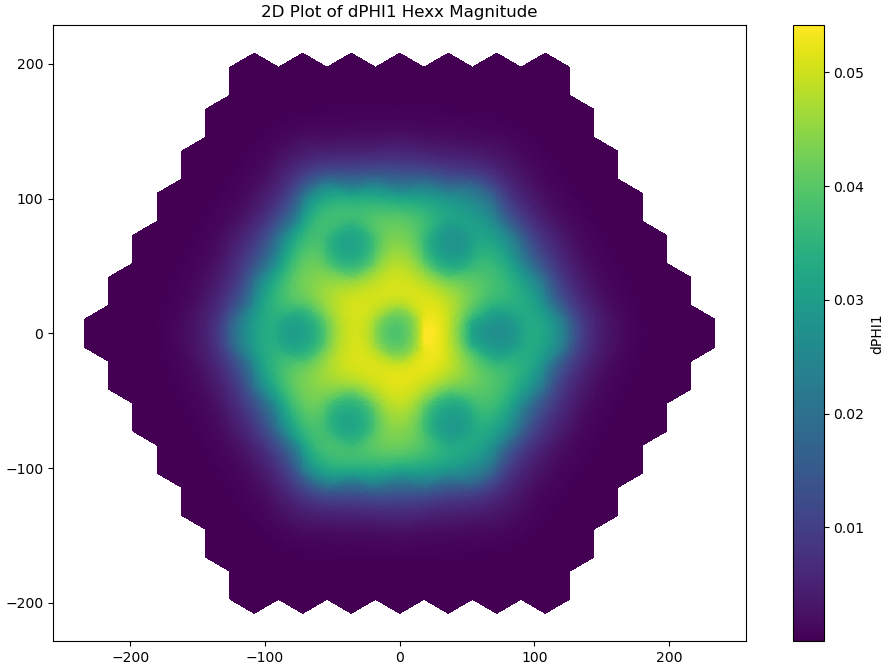
\includegraphics[width=\linewidth]{figures/OBJECTIVES3_TEST04_2DTriMG_HTTR2G_FAV_level5_NOISE_dPHI_magnitude_G1.png}
        \end{subfigure}
        \hfill
        \begin{subfigure}{.48\textwidth}
          \centering
          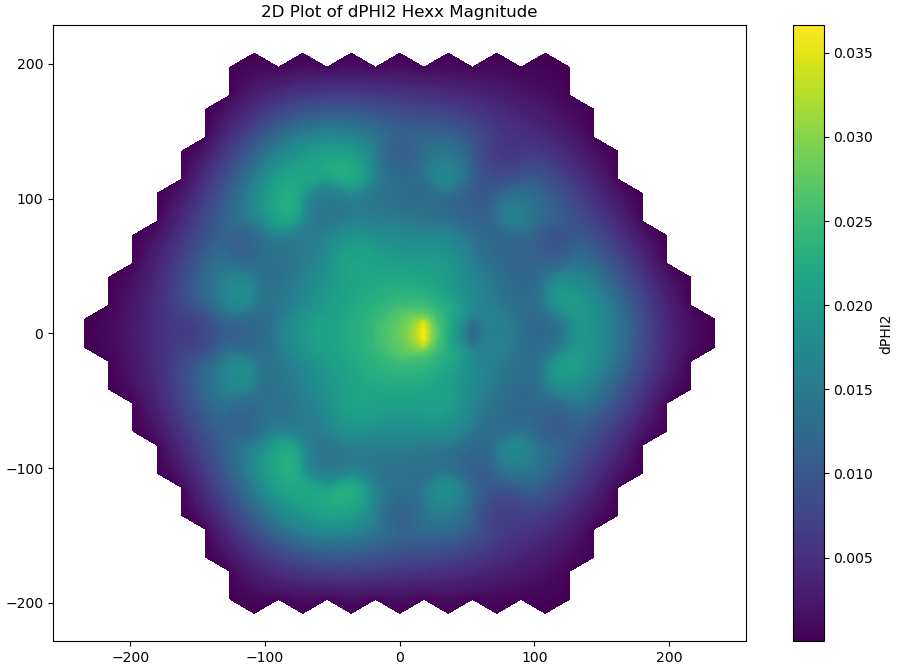
\includegraphics[width=\linewidth]{figures/OBJECTIVES3_TEST04_2DTriMG_HTTR2G_FAV_level5_NOISE_dPHI_magnitude_G2.png}
        \end{subfigure}
        \caption{Magnitude of the neutron noise for FAV in 2D HTTR}
        \label{fig:2DHTTR_noise_FAV_results_mag}
\end{figure}
\begin{figure}[H]
        \centering
        \begin{subfigure}{.48\textwidth}
          \centering
          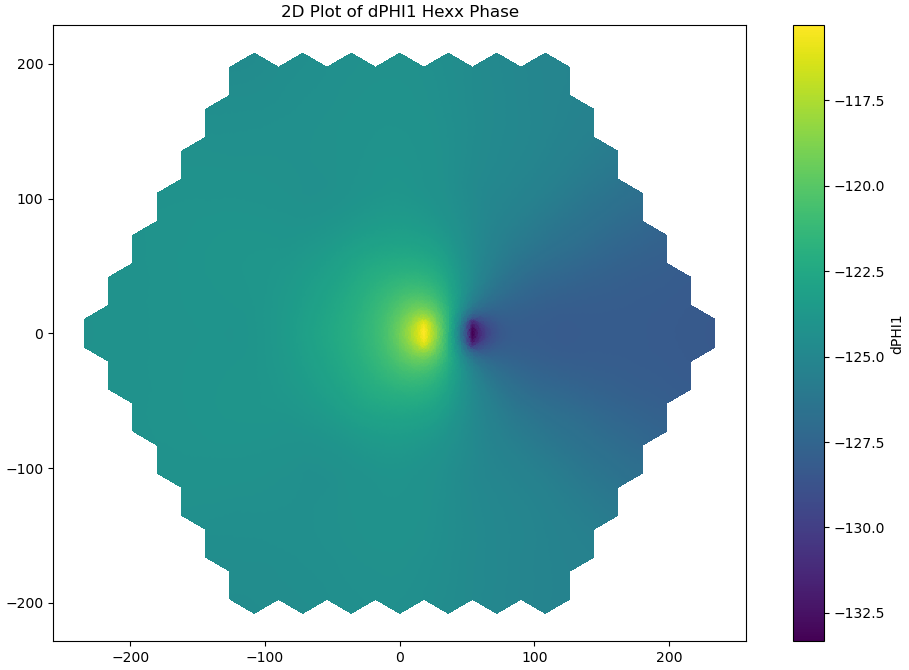
\includegraphics[width=\linewidth]{figures/OBJECTIVES3_TEST04_2DTriMG_HTTR2G_FAV_level5_NOISE_dPHI_phase_G1.png}
        \end{subfigure}
        \hfill
        \begin{subfigure}{.48\textwidth}
          \centering
          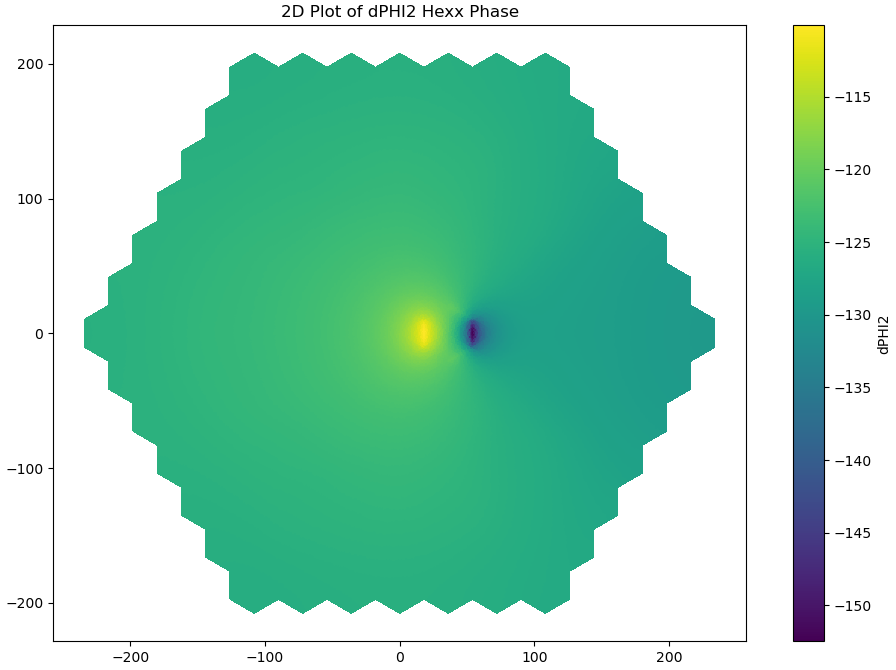
\includegraphics[width=\linewidth]{figures/OBJECTIVES3_TEST04_2DTriMG_HTTR2G_FAV_level5_NOISE_dPHI_phase_G2.png}
        \end{subfigure}
        \caption{Phase of the neutron noise for FAV in 2D HTTR}
        \label{fig:2DHTTR_noise_FAV_results_phase}
\end{figure}

As seen in Figure \ref{fig:2DHTTR_noise_FAV_results_mag} and Figure \ref{fig:2DHTTR_noise_FAV_results_phase}, the neutron noise is more apparent in the thermal group and more dispersed in the fast group. This is a similar phenomenon compared to the AVS source in 2D HTTR. For the fuel assembly vibration case, it is expected that there will be some opposing effect in the magnitude and phase delay results due to the out-of-phase neutron noise source model. This is clearly evident in the simulation. Since the vibrating assembly is a fuel assembly, the opposing effect is not so apparent in the interfaces where the neighboring assembly is also a fuel assembly. This is expected since the difference between the macroscopic cross-sections  ($\Delta \Sigma_{a,g}$) is smaller at these interfaces. However, the opposing effect becomes more evident at the interfaces where the neighboring assembly is a reflector assembly. 

To further understand the driving force of neutron noise, we can split the neutron noise into its point kinetic component and its spatial component. Figures \ref{fig:2DHTTRFAV_noise_component_results1} and \ref{fig:2DHTTRFAV_noise_component_results2} show the point kinetic component and spatial component of the neutron noise in fast and thermal group with FAV source, taken at the centerline of the core ($y=0$).

\begin{figure}[H]
        \centering
        \begin{subfigure}{.48\textwidth}
          \centering
          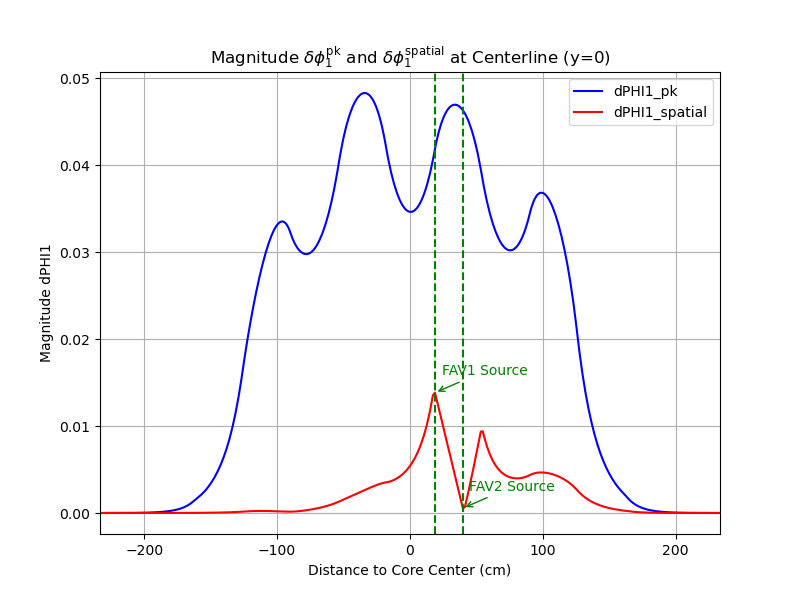
\includegraphics[width=\linewidth]{figures/Centerline_y0_OBJECTIVES3_TEST04_2DTriMG_HTTR2G_FAV_level5_dPHI_magnitude_G1.png}
        \end{subfigure}
        \hfill
        \begin{subfigure}{.48\textwidth}
          \centering
          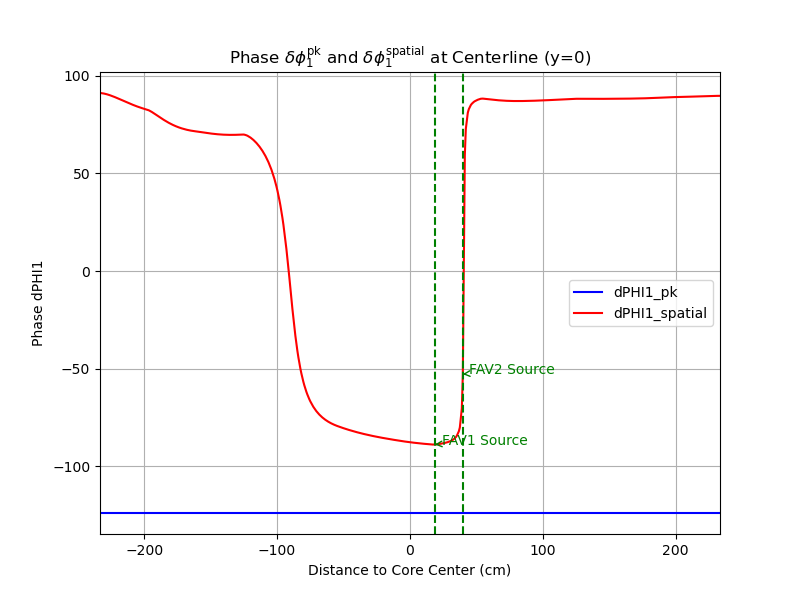
\includegraphics[width=\linewidth]{figures/Centerline_y0_OBJECTIVES3_TEST04_2DTriMG_HTTR2G_FAV_level5_dPHI_phase_G1.png}
        \end{subfigure}
        \caption{Magnitude (left) and phase (right) of the components of fast neutron noise for FAV in 2D HTTR, taken at centerline ($y=0$)}
        \label{fig:2DHTTRFAV_noise_component_results1}
\end{figure}
\begin{figure}[H]
        \centering
        \begin{subfigure}{.48\textwidth}
          \centering
          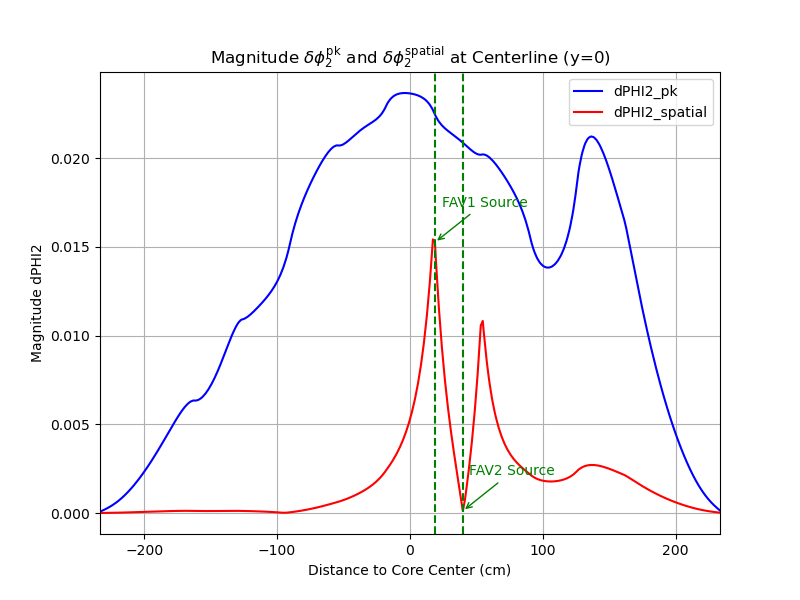
\includegraphics[width=\linewidth]{figures/Centerline_y0_OBJECTIVES3_TEST04_2DTriMG_HTTR2G_FAV_level5_dPHI_magnitude_G2.png}
        \end{subfigure}
        \hfill
        \begin{subfigure}{.48\textwidth}
          \centering
          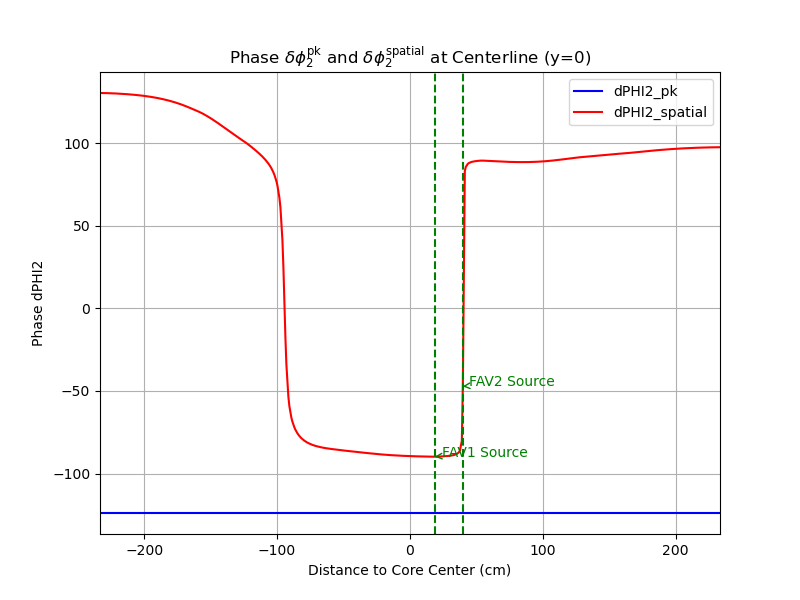
\includegraphics[width=\linewidth]{figures/Centerline_y0_OBJECTIVES3_TEST04_2DTriMG_HTTR2G_FAV_level5_dPHI_phase_G2.png}
        \end{subfigure}
        \caption{Magnitude (left) and phase (right) of the components of thermal neutron noise for FAV in 2D HTTR, taken at centerline ($y=0$)}
        \label{fig:2DHTTRFAV_noise_component_results2}
\end{figure}
Comparing Figure \ref{fig:2DHTTRFAV_noise_component_results1}, and Figure \ref{fig:2DHTTRFAV_noise_component_results2}, we can see that the behavior is similar to the AVS source, where the point kinetic component is more apparent in the magnitude of neutron noise. The point kinetic component in the fast group is more dominant compared to the thermal group, which makes the magnitude of the neutron noise in the fast group more dispersed. The opposing effect of the neutron noise source is reflected in the magnitude of the neutron noise source. The spatial component influences the phase delays similarly to the AVS source. The out-of-phase behavior can be clearly seen in the phases of the neutron noise. In general, we can see that the point kinetic component has a more significant impact on the magnitude of neutron noise, while the spatial component affects the phase of the neutron noise. 

\subsection{3D HTTR with Absorber of Variable Strength Source}

For this simulation, the neutron noise source is defined as perturbation of the thermal absorption cross-section in the fuel assembly. Formally, the perturbation can be written as follows:
\begin{equation}
    \delta \Sigma_{a,2}(\textbf{r}, \omega) = \gamma(\omega) \delta(\textbf{r} - \textbf{r}_0)
\end{equation}
Where $\gamma(\omega)$ is defined as 5\% of the thermal absorption cross-section at $r_0$ and $r_0$ is defined as one triangle mesh in assembly number 65 at mid-elevation (mid-elevation of fuel zone 1, indicated as red triangle), which is shown in Figure \ref{fig:HTTR3DAVS}.
\begin{figure}[H]
        \centering
        \begin{subfigure}{.48\textwidth}
          \centering
          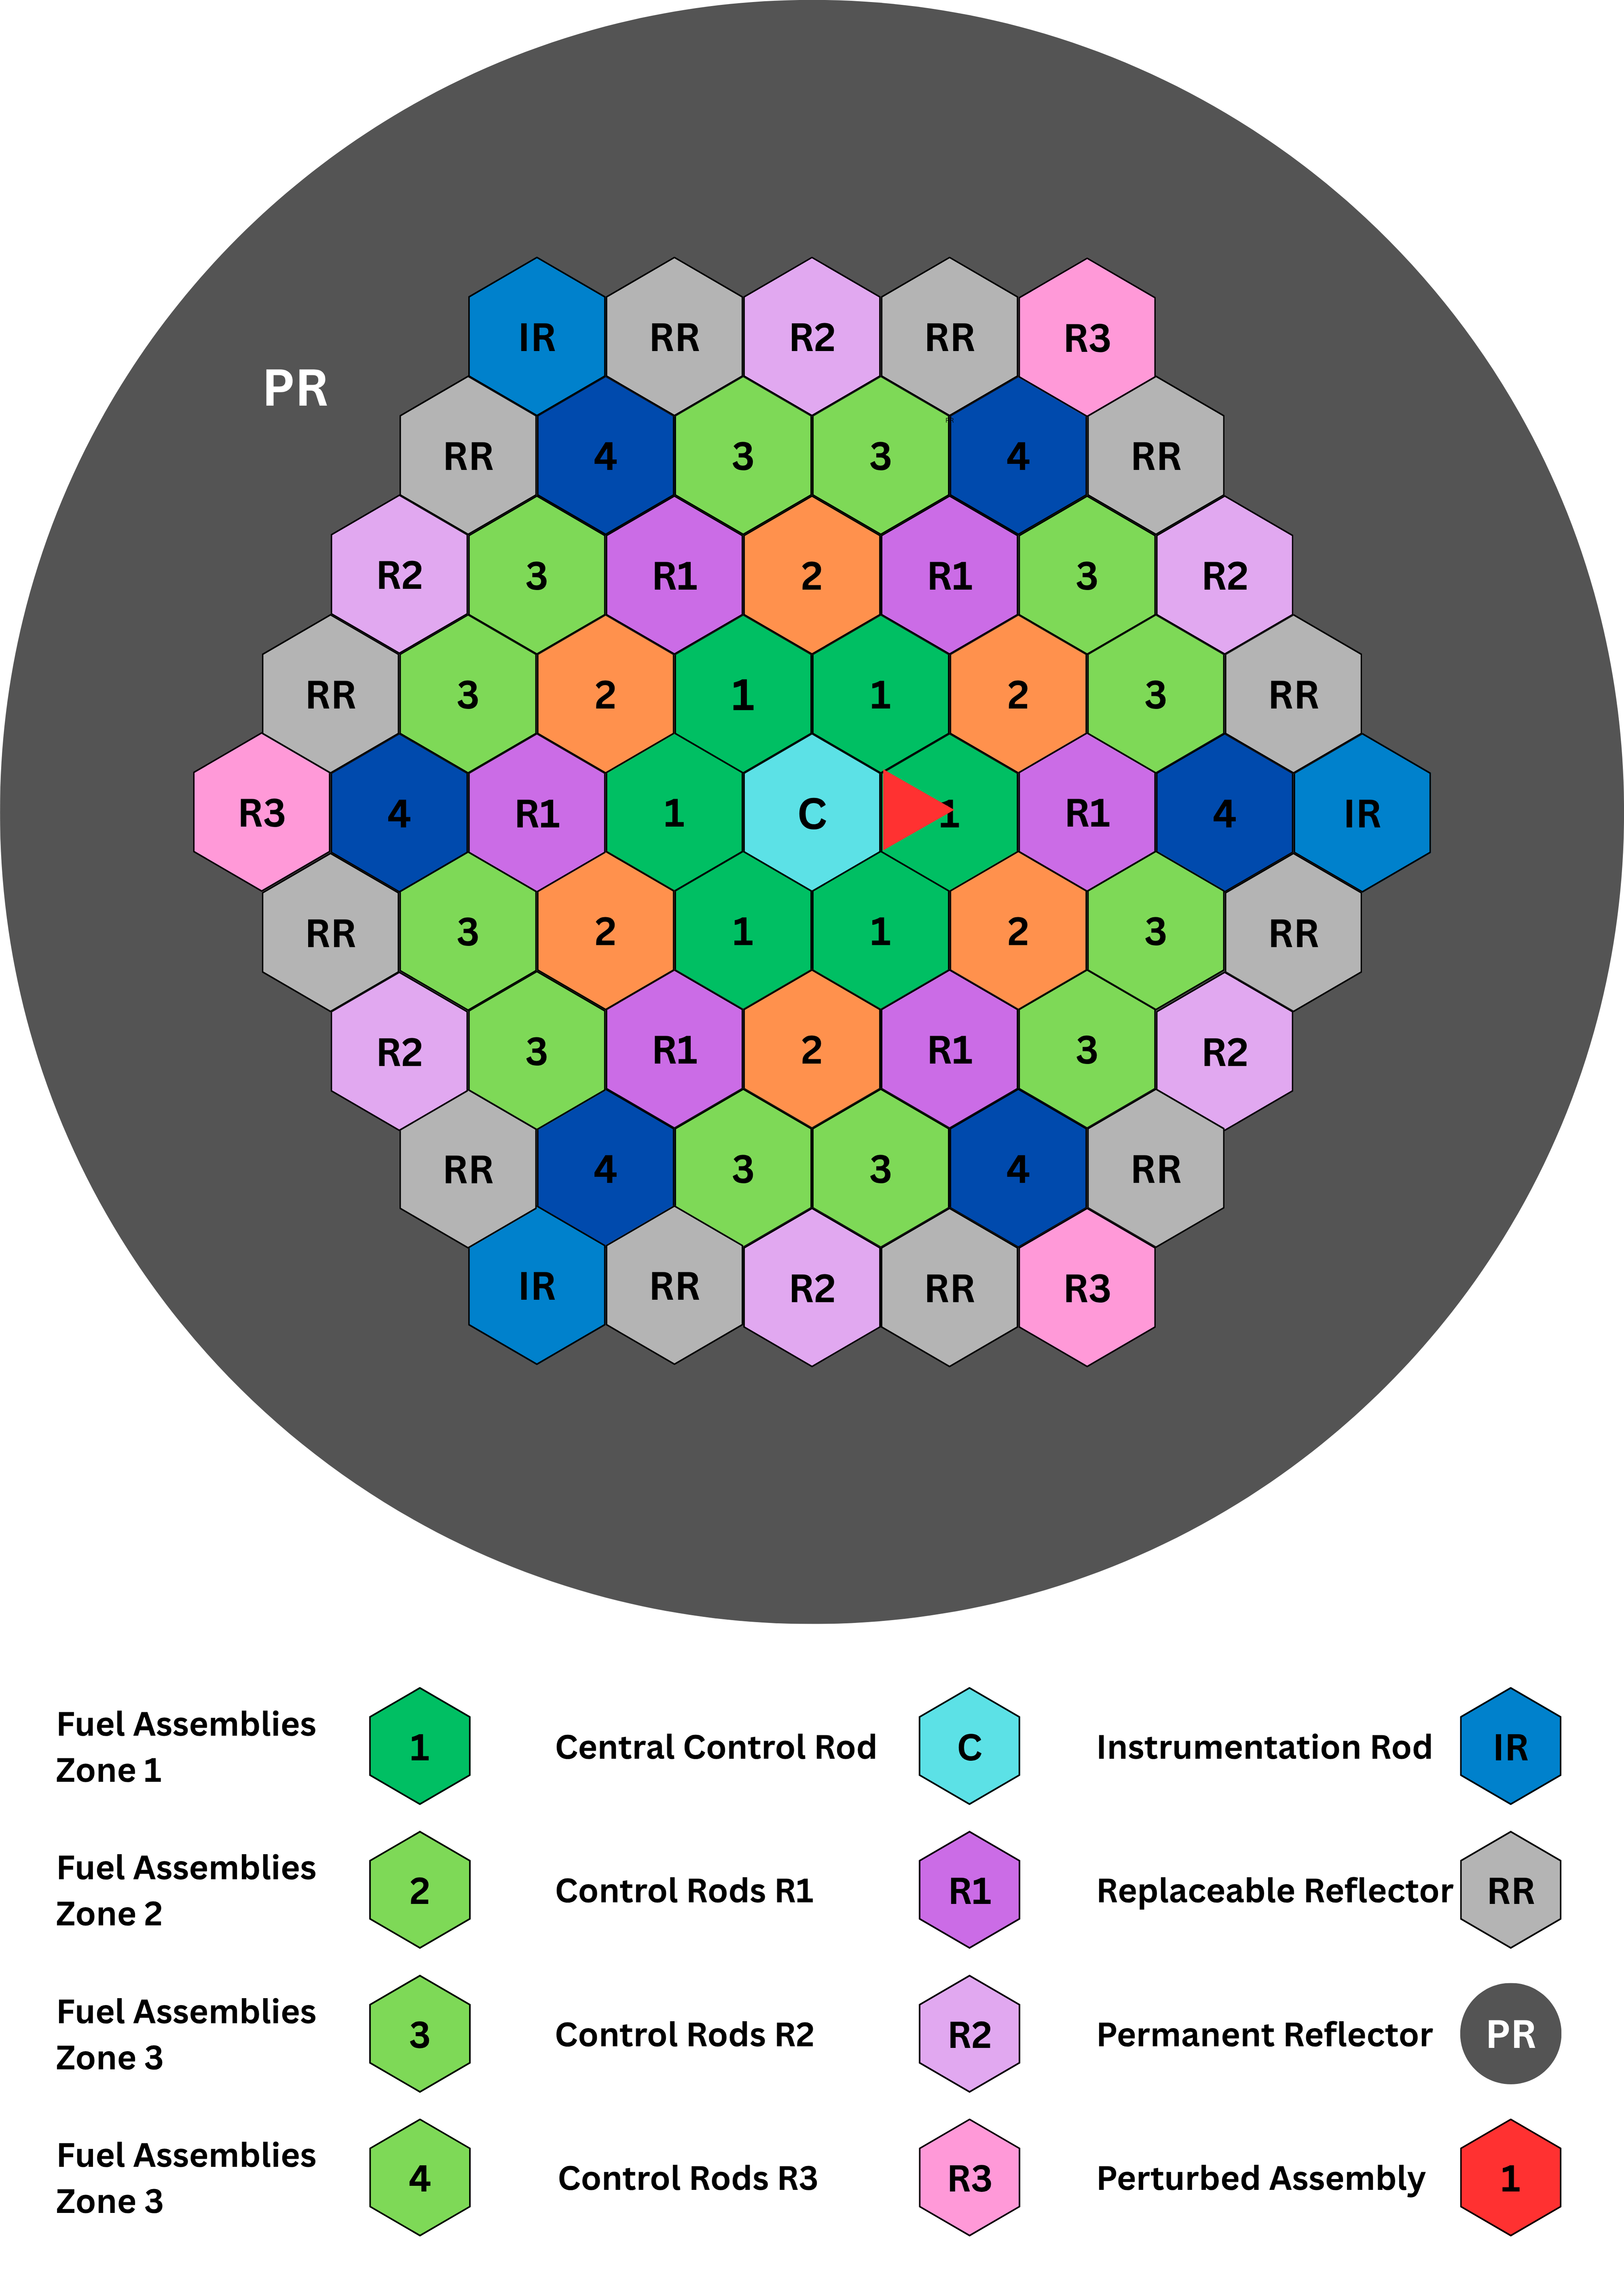
\includegraphics[width=\linewidth]{figures/HTTR3DAVS1.png}
        \end{subfigure}
        \hfill
        \begin{subfigure}{.48\textwidth}
          \centering
          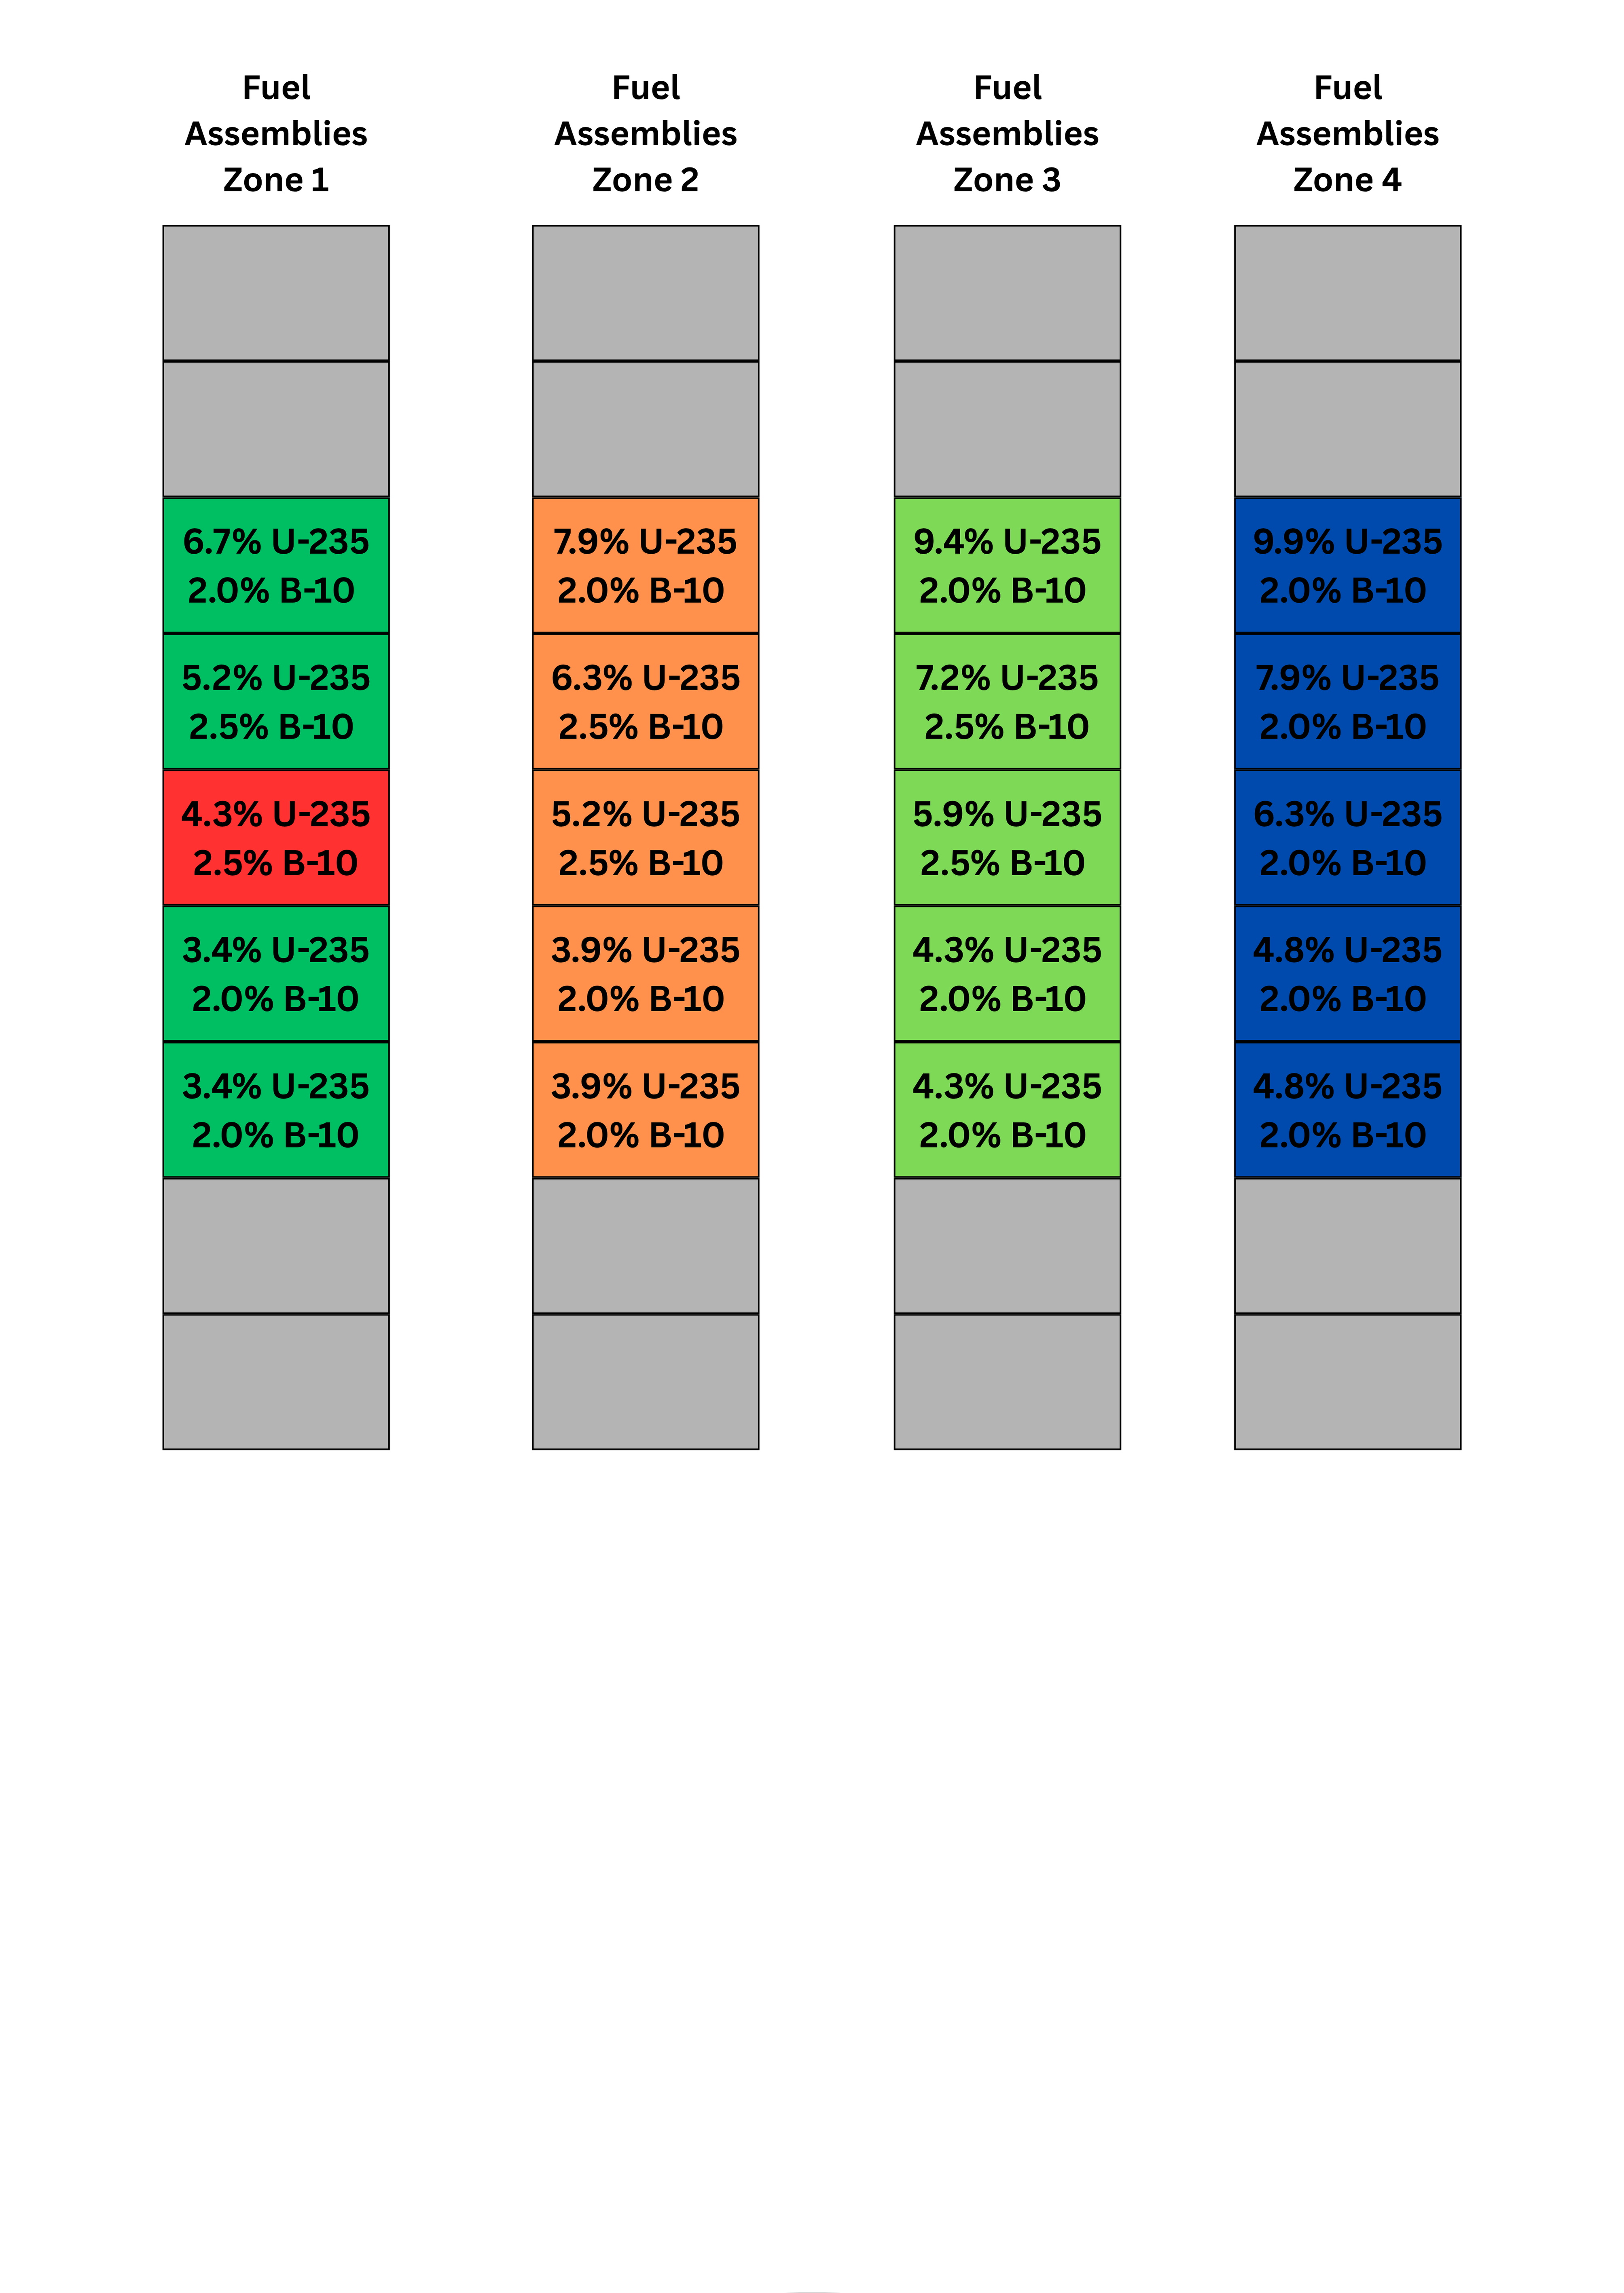
\includegraphics[width=\linewidth]{figures/HTTR3DAVS2.png}
        \end{subfigure}
        \caption{Location of the absorber of variable strength for 3D HTTR}
        \label{fig:HTTR3DAVS}
\end{figure}

The results of the simulations are as follows:
\begin{figure}[H]
        \centering
        \begin{subfigure}{.48\textwidth}
          \centering
          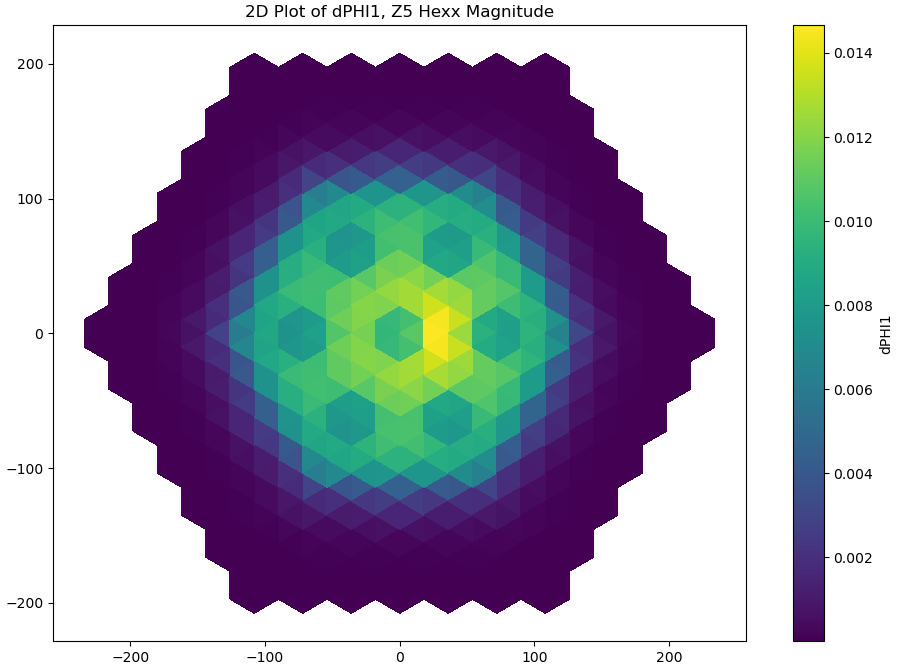
\includegraphics[width=\linewidth]{figures/OBJECTIVES3_TEST07_3DTriMG_HTTR_AVS_level1_NOISE_dPHI_magnitude_G1_Z5.png}
        \end{subfigure}
        \hfill
        \begin{subfigure}{.48\textwidth}
          \centering
          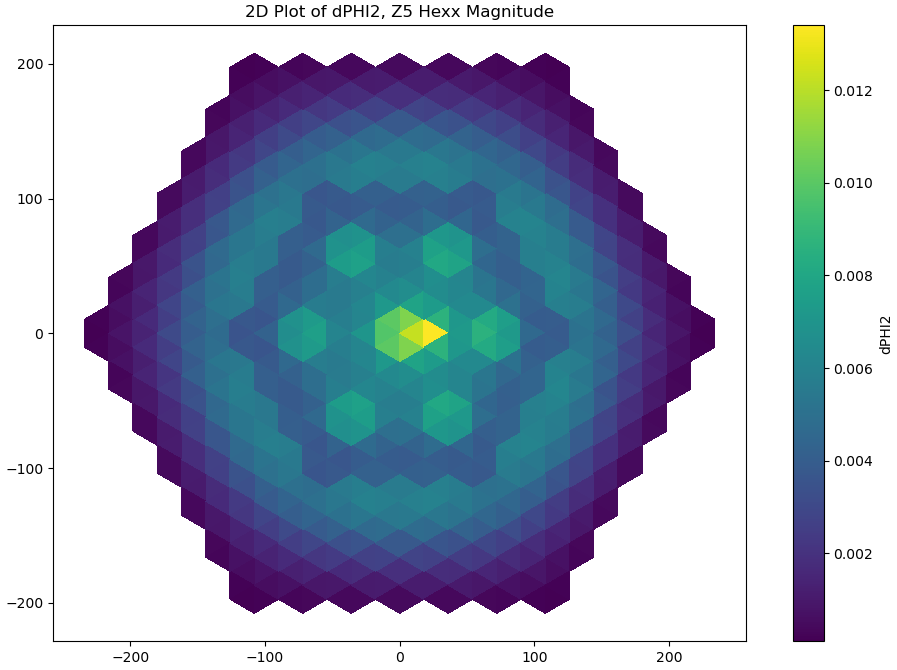
\includegraphics[width=\linewidth]{figures/OBJECTIVES3_TEST07_3DTriMG_HTTR_AVS_level1_NOISE_dPHI_magnitude_G2_Z5.png}
        \end{subfigure}
        \caption{Magnitude of the neutron noise for AVS in 3D HTTR at midplane ($Z = 5$)}
        \label{fig:3DHTTR_noise_AVS_results_mag}
\end{figure}
\begin{figure}[H]
        \centering
        \begin{subfigure}{.48\textwidth}
          \centering
          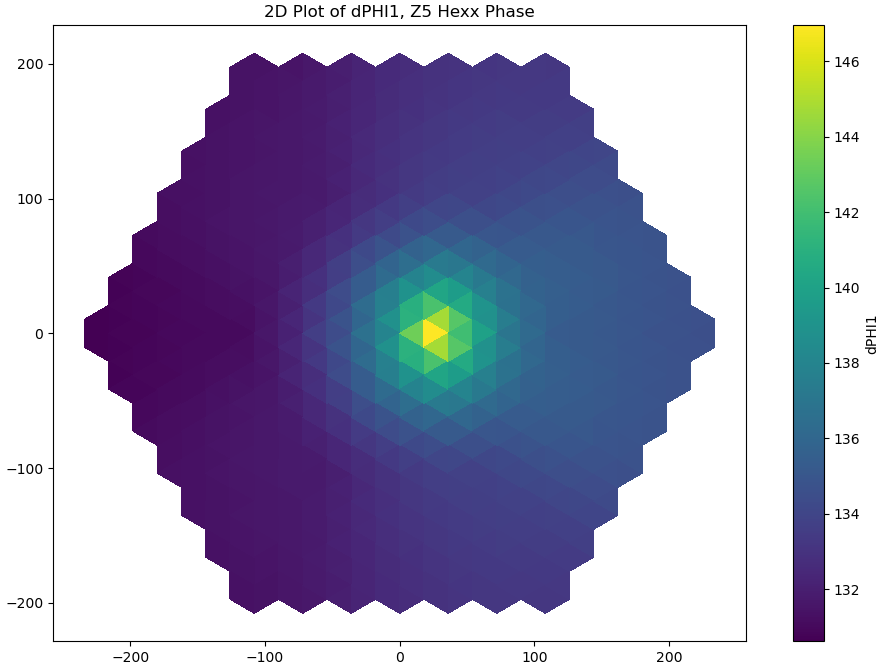
\includegraphics[width=\linewidth]{figures/OBJECTIVES3_TEST07_3DTriMG_HTTR_AVS_level1_NOISE_dPHI_phase_G1_Z5.png}
        \end{subfigure}
        \hfill
        \begin{subfigure}{.48\textwidth}
          \centering
          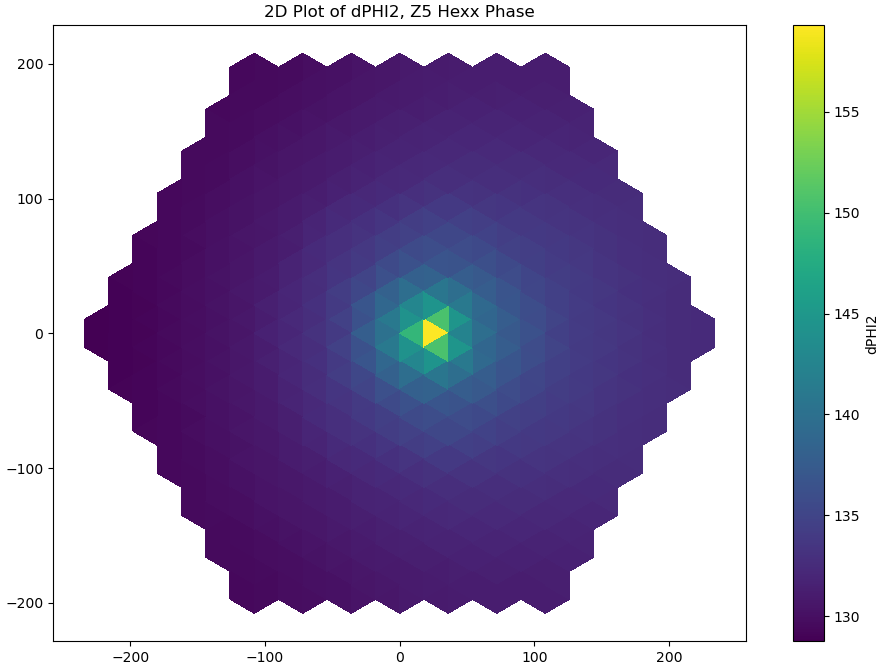
\includegraphics[width=\linewidth]{figures/OBJECTIVES3_TEST07_3DTriMG_HTTR_AVS_level1_NOISE_dPHI_phase_G2_Z5.png}
        \end{subfigure}
        \caption{Phase of the neutron noise for AVS in 3D HTTR at midplane ($Z = 5$)}
        \label{fig:3DHTTR_noise_AVS_results_phase}
\end{figure}

As shown in Figures \ref{fig:3DHTTR_noise_AVS_results_mag} and \ref{fig:3DHTTR_noise_AVS_results_phase}, the effect of neutron noise is more pronounced in the thermal group. This is mainly due to the noise source located in the thermal spectrum only. We can also see in the phase delay plot (Figure \ref{fig:3DHTTR_noise_AVS_results_phase}) that the effect of neutron noise is more localized in the thermal group compared to the fast group. This behavior is generally similar to the 2D HTTR case.

To further understand the driving force of neutron noise, we can split the neutron noise into its point kinetic component and its spatial component. Figures \ref{fig:3DHTTRAVS_noise_component_results1} and \ref{fig:3DHTTRAVS_noise_component_results2} show the point kinetic component and spatial component of the neutron noise in fast and thermal group with AVS source, taken at the centerline of the core ($y=0$) and midplane ($Z = 5$).

\begin{figure}[H]
        \centering
        \begin{subfigure}{.48\textwidth}
          \centering
          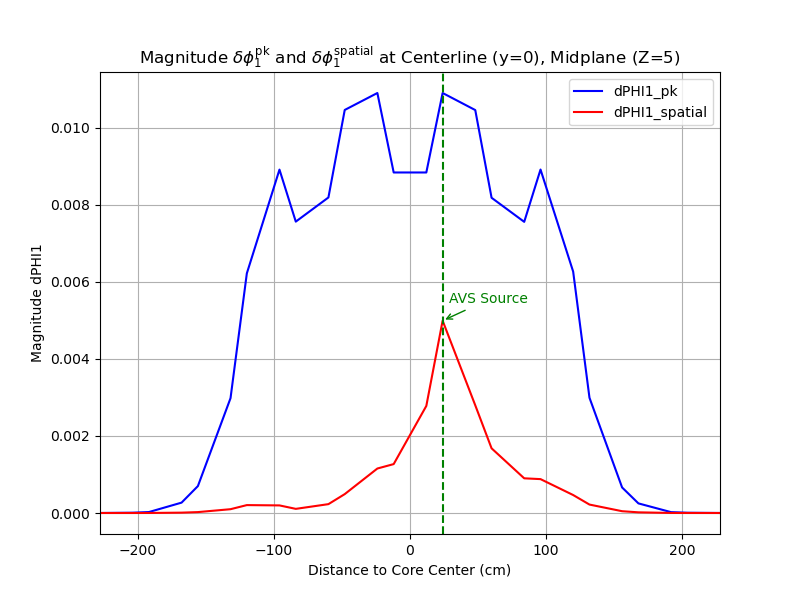
\includegraphics[width=\linewidth]{figures/Centerline_y0_OBJECTIVES3_TEST07_3DTriMG_HTTR_AVS_level1_dPHI_magnitude_G1.png}
        \end{subfigure}
        \hfill
        \begin{subfigure}{.48\textwidth}
          \centering
          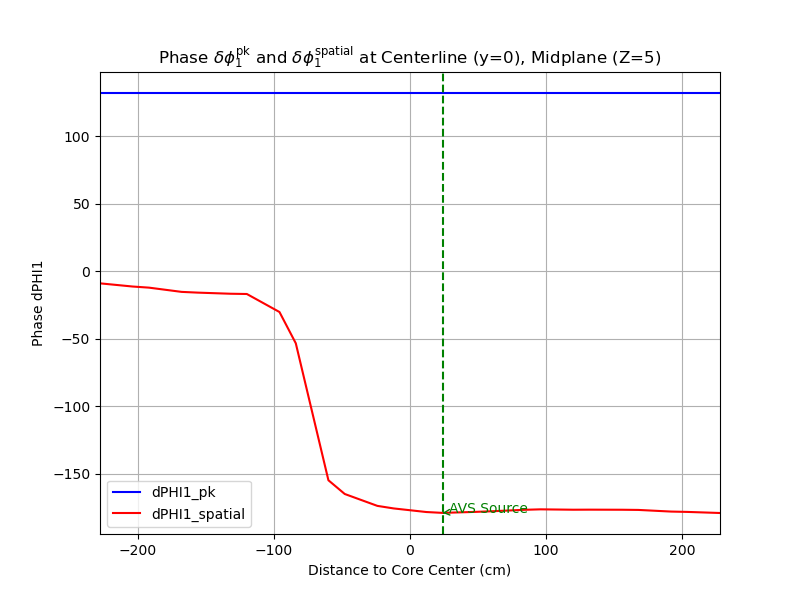
\includegraphics[width=\linewidth]{figures/Centerline_y0_OBJECTIVES3_TEST07_3DTriMG_HTTR_AVS_level1_dPHI_phase_G1.png}
        \end{subfigure}
        \caption{Magnitude (left) and phase (right) of the components of fast neutron noise for AVS in 3D HTTR at centerline ($y=0$), midplane ($Z=5$)}
        \label{fig:3DHTTRAVS_noise_component_results1}
\end{figure}
\begin{figure}[H]
        \centering
        \begin{subfigure}{.48\textwidth}
          \centering
          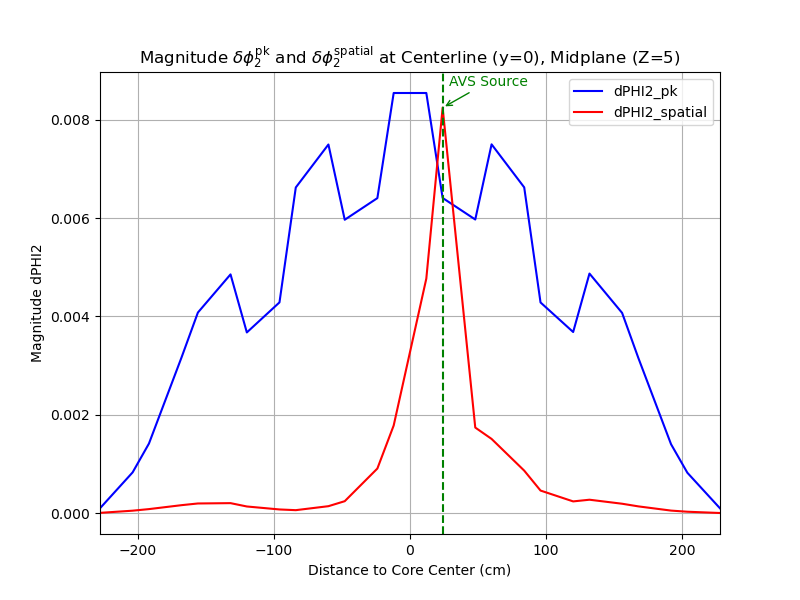
\includegraphics[width=\linewidth]{figures/Centerline_y0_OBJECTIVES3_TEST07_3DTriMG_HTTR_AVS_level1_dPHI_magnitude_G2.png}
        \end{subfigure}
        \hfill
        \begin{subfigure}{.48\textwidth}
          \centering
          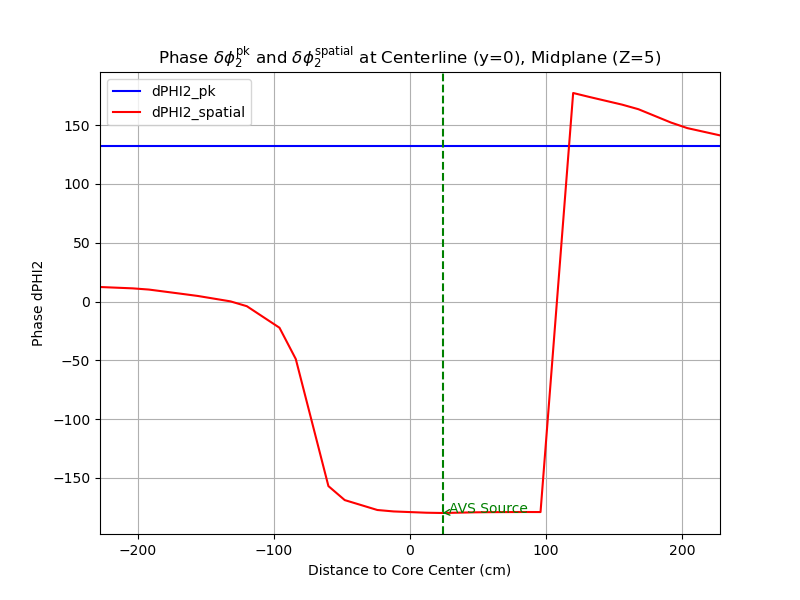
\includegraphics[width=\linewidth]{figures/Centerline_y0_OBJECTIVES3_TEST07_3DTriMG_HTTR_AVS_level1_dPHI_phase_G2.png}
        \end{subfigure}
        \caption{Magnitude (left) and phase (right) of the components of thermal neutron noise for AVS in 3D HTTR at centerline ($y=0$), midplane ($Z=5$)}
        \label{fig:3DHTTRAVS_noise_component_results2}
\end{figure}

Comparing Figure \ref{fig:3DHTTRAVS_noise_component_results1} and Figure \ref{fig:3DHTTRAVS_noise_component_results2}, we can see that in the fast group, the magnitude of the point kinetic component is more dominant compared to the spatial component. However, in the thermal group, the magnitude of the point kinetic component is lower at the AVS source location. This makes the contribution of the spatial component more apparent in the thermal group. The variation of the phase delay is mainly driven by the spatial components. It is expected that the point kinetic component will have no effect on the phase delays since it is a factor of the forward flux. Overall, we can see that the point kinetic component is more dominant in 3D HTTR compared to the spatial component, which means that the neutron noise is driven by the reactivity effect of the perturbation.

\subsection{3D HTTR with Fuel Assembly Vibration Source}

For the simulation of the fuel assembly vibration, the neutron noise source is modeled using the $\varepsilon/d$ method, similar to the 2D HTTR case. In this case, the frequency of vibration ($\omega_0$) is defined as 1 Hz, and the amplitude of vibration ($\varepsilon$) is 0.5 cm. Using this definition, the neutron noise source model is written as follows:
\begin{equation}
    \delta \Sigma_{a,g} (\textbf{r}_b, z ,\omega) = \left\{
\begin{array}{ll}
      -i \pi \varepsilon \Delta  \Sigma_{a,g} \delta (\omega - \omega_0) & \textbf{r}_b-\varepsilon\leq y \leq \textbf{r}_b + \varepsilon \\
      0 & \text{otherwise}\\
\end{array} 
\right. 
\end{equation}
This means that all the interfaces of the assembly become the source of neutron noise. The vibration is located at assembly number 65 along the $z$-axis, as shown in Figure \ref{fig:3DHTTRFAV}.
\begin{figure}[H]
        \centering
        \begin{subfigure}{.48\textwidth}
          \centering
          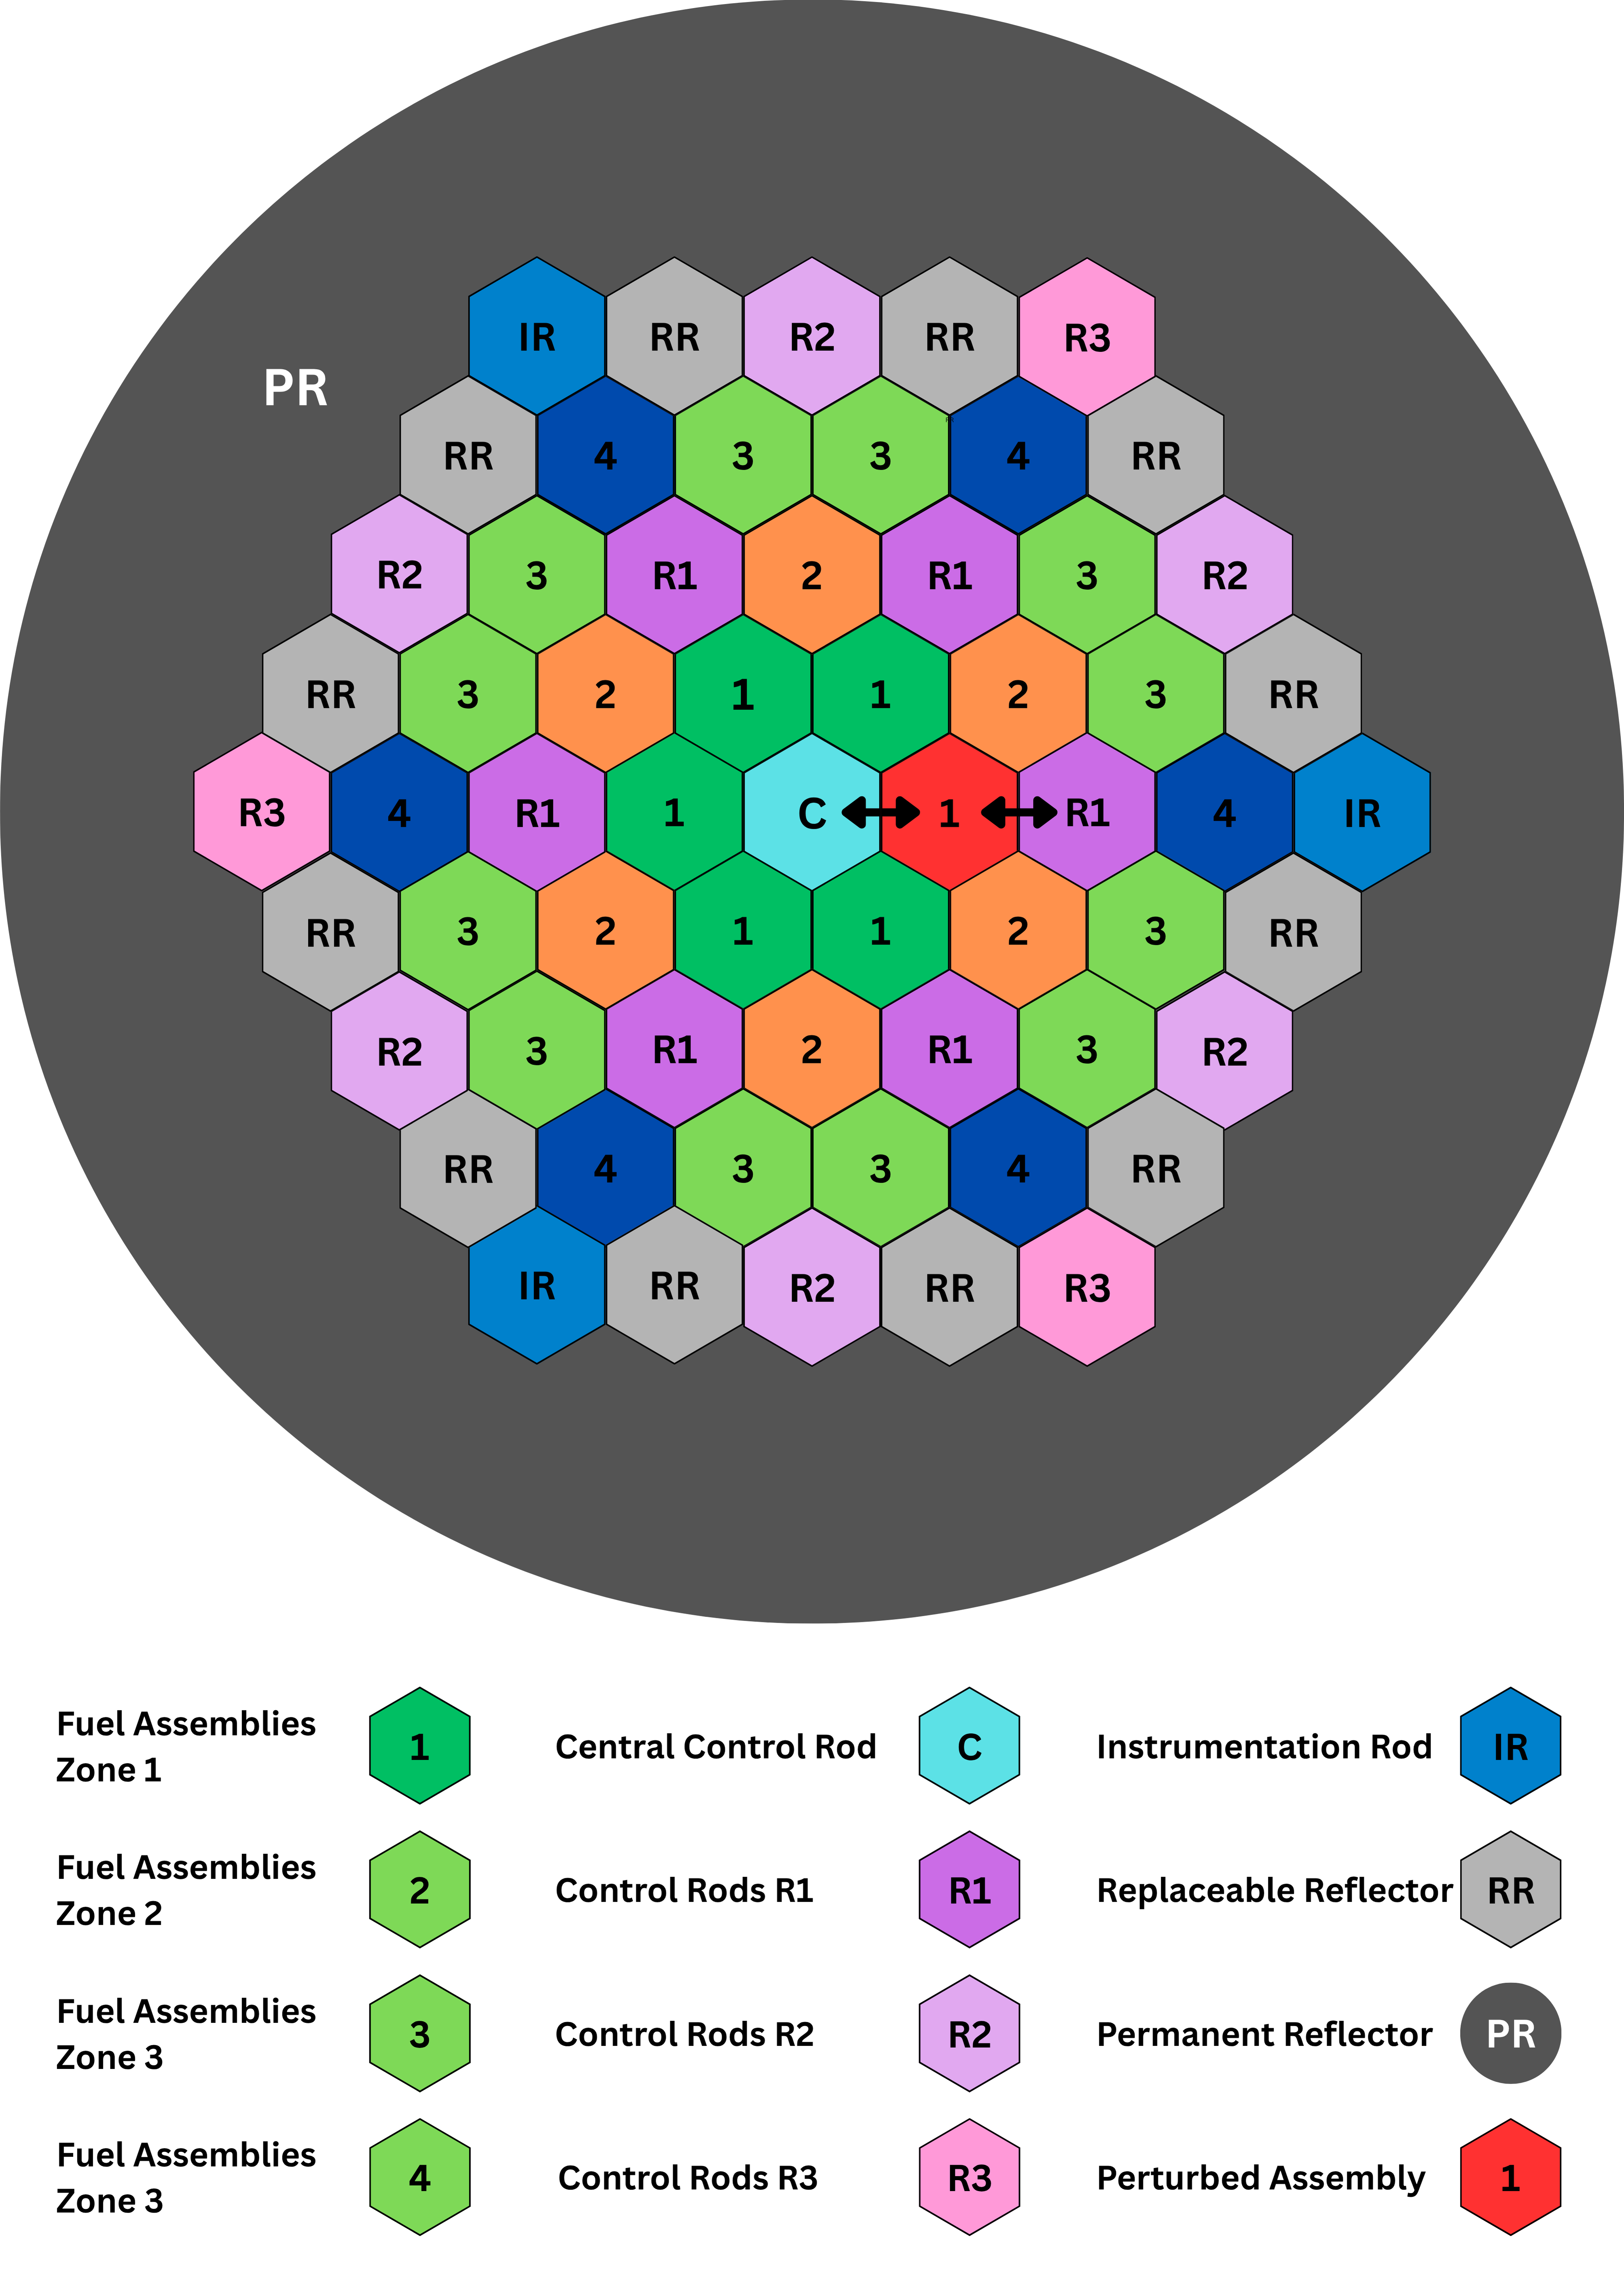
\includegraphics[width=\linewidth]{figures/HTTR3DFAV1.png}
        \end{subfigure}
        \hfill
        \begin{subfigure}{.48\textwidth}
          \centering
          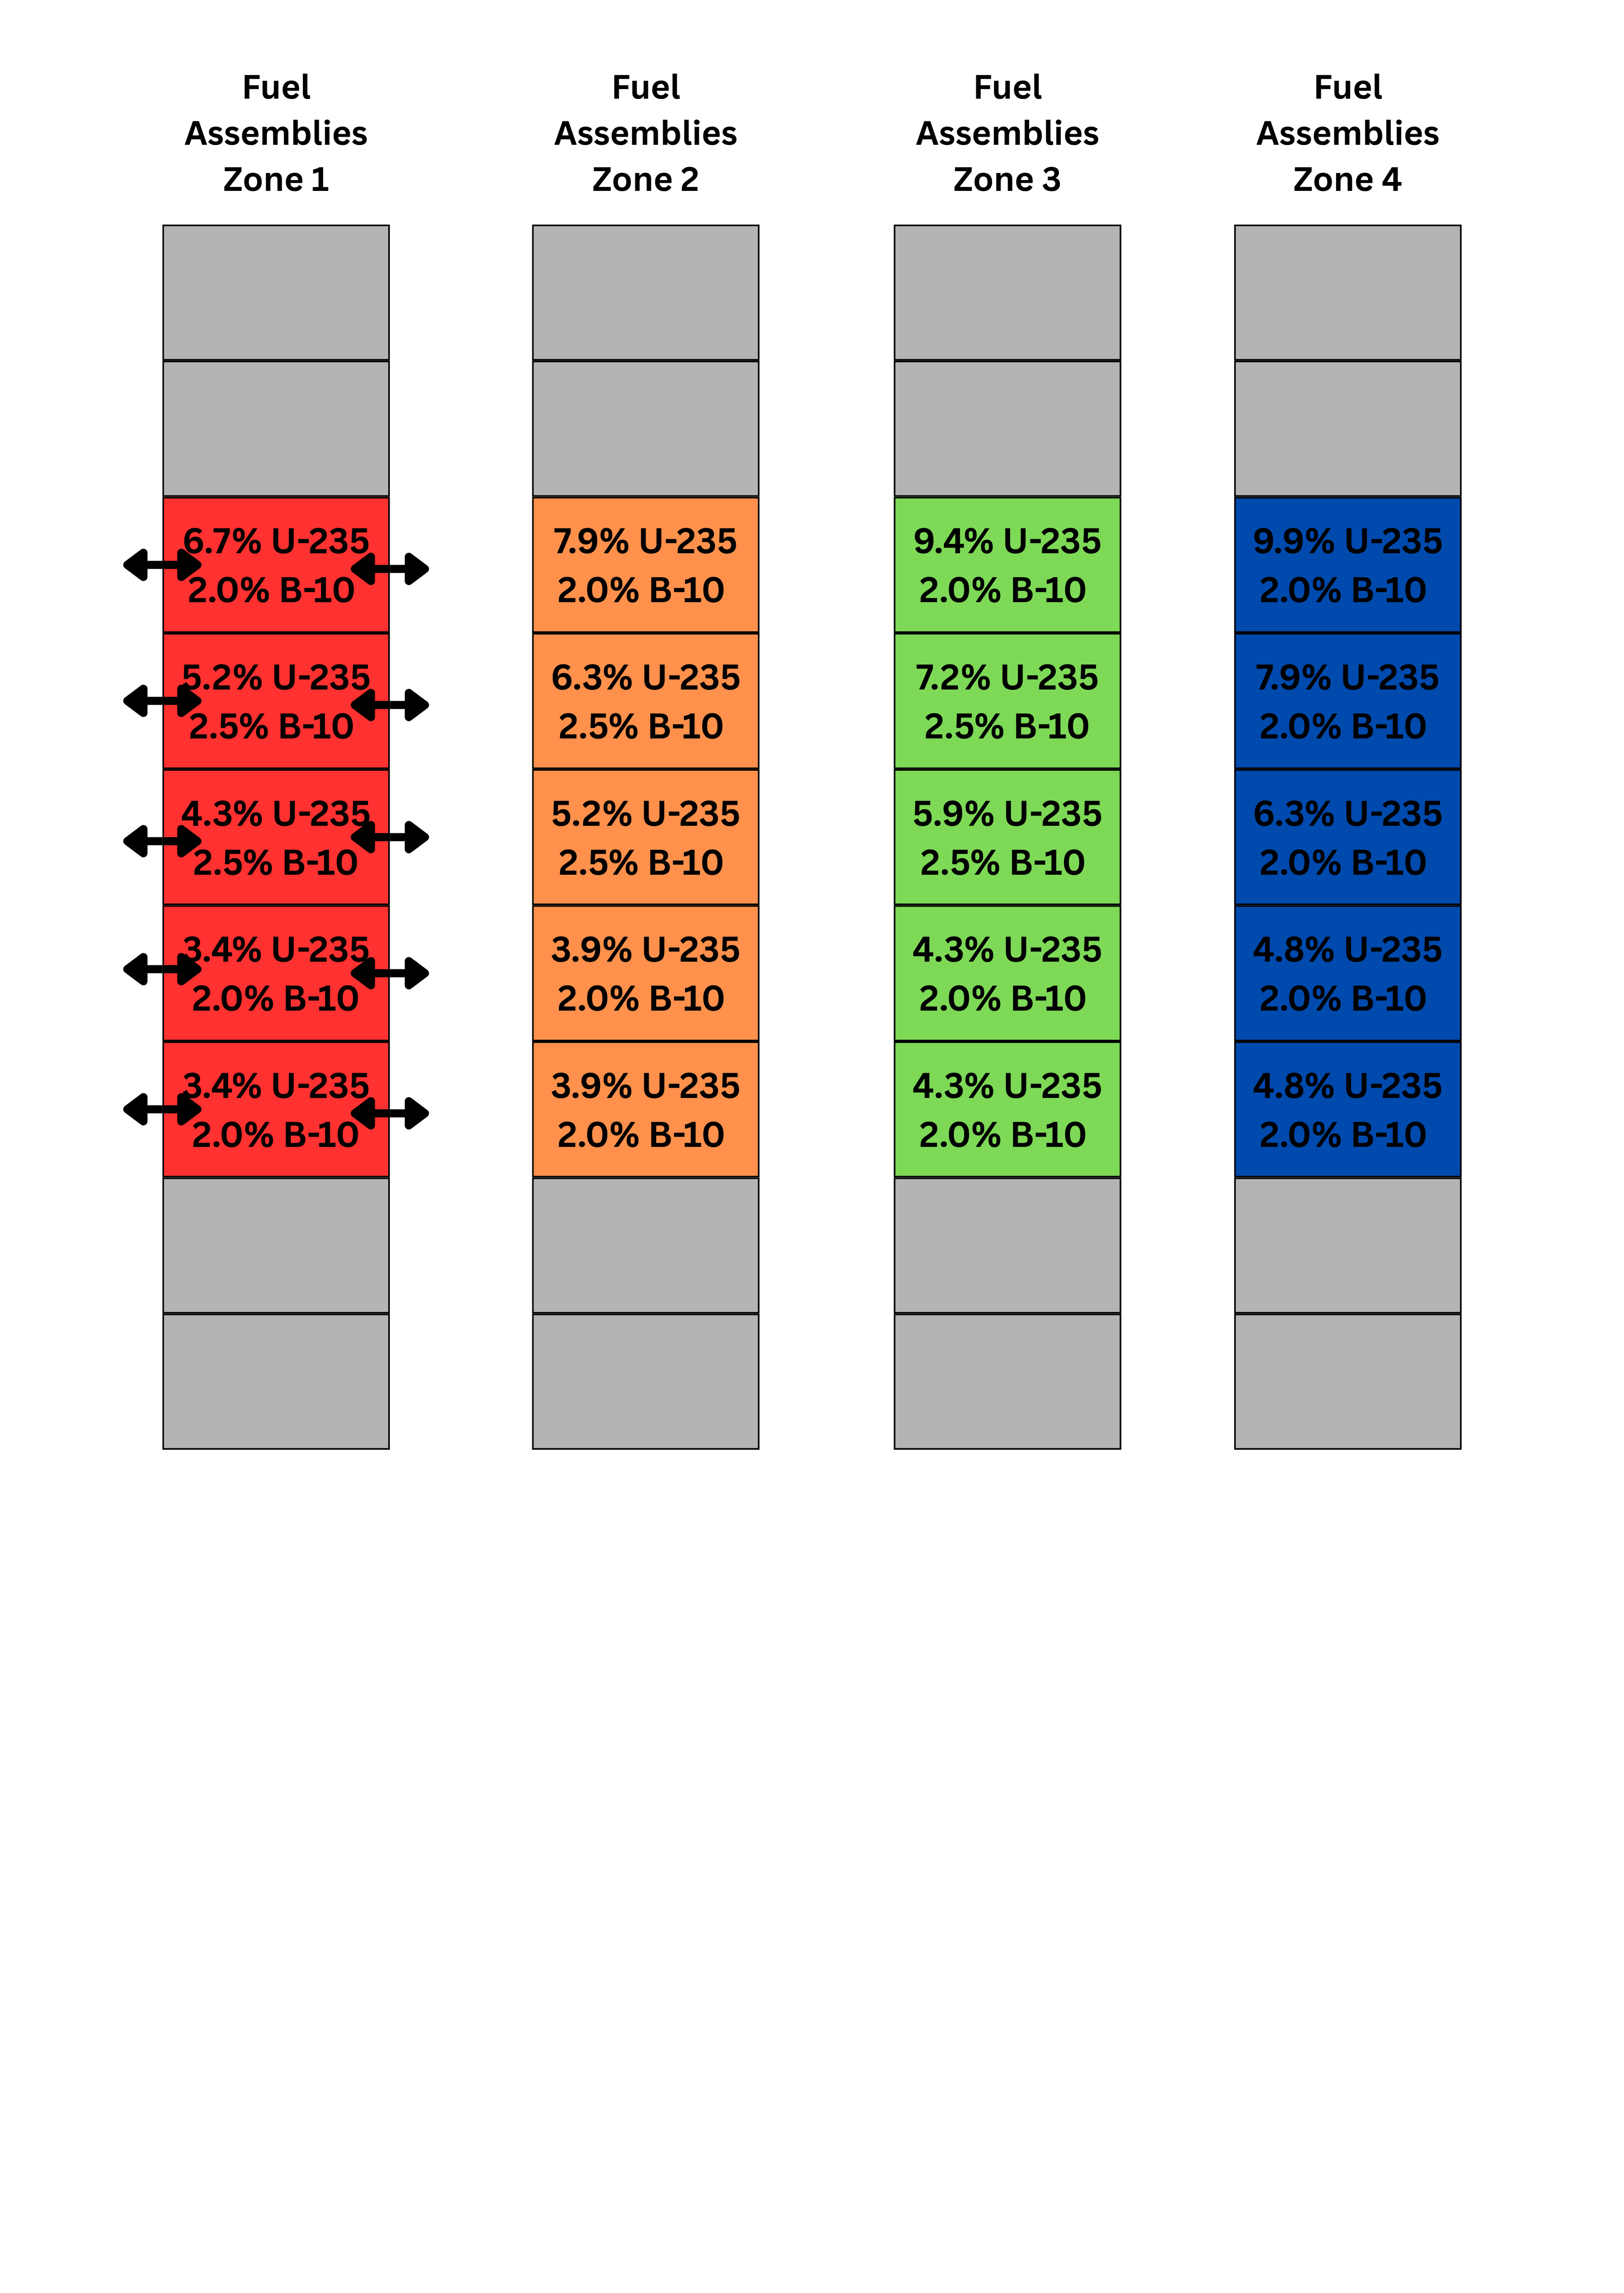
\includegraphics[width=\linewidth]{figures/HTTR3DFAV2.png}
        \end{subfigure}
        \caption{Location of the fuel assembly vibration for 3D HTTR}
        \label{fig:3DHTTRFAV}
\end{figure}

The results of the simulations are as follows:
\begin{figure}[H]
        \centering
        \begin{subfigure}{.48\textwidth}
          \centering
          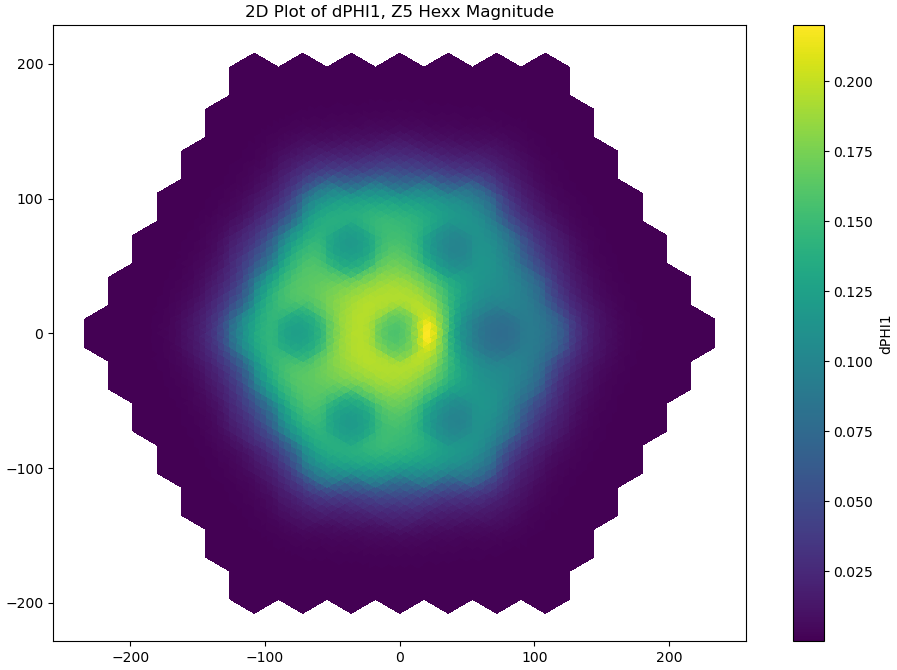
\includegraphics[width=\linewidth]{figures/OBJECTIVES3_TEST08_3DTriMG_HTTR_FAV_level3_NOISE_dPHI_magnitude_G1_Z5.png}
        \end{subfigure}
        \hfill
        \begin{subfigure}{.48\textwidth}
          \centering
          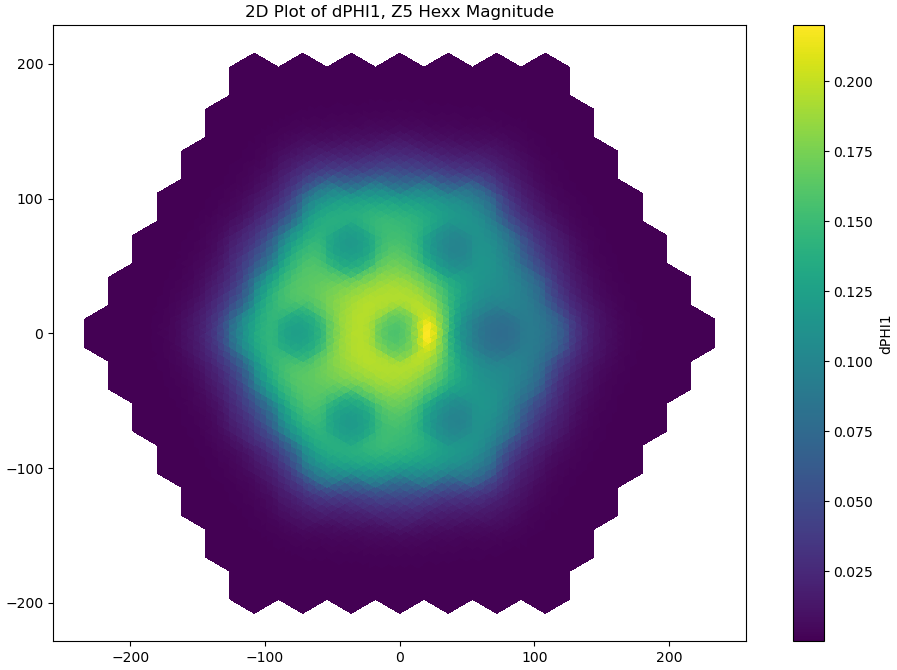
\includegraphics[width=\linewidth]{figures/OBJECTIVES3_TEST08_3DTriMG_HTTR_FAV_level3_NOISE_dPHI_magnitude_G1_Z5.png}
        \end{subfigure}
        \caption{Magnitude of the neutron noise for FAV in 3D HTTR at midplane ($Z = 5$)}
        \label{fig:3DHTTR_noise_FAV_results_mag}
\end{figure}
\begin{figure}[H]
        \centering
        \begin{subfigure}{.48\textwidth}
          \centering
          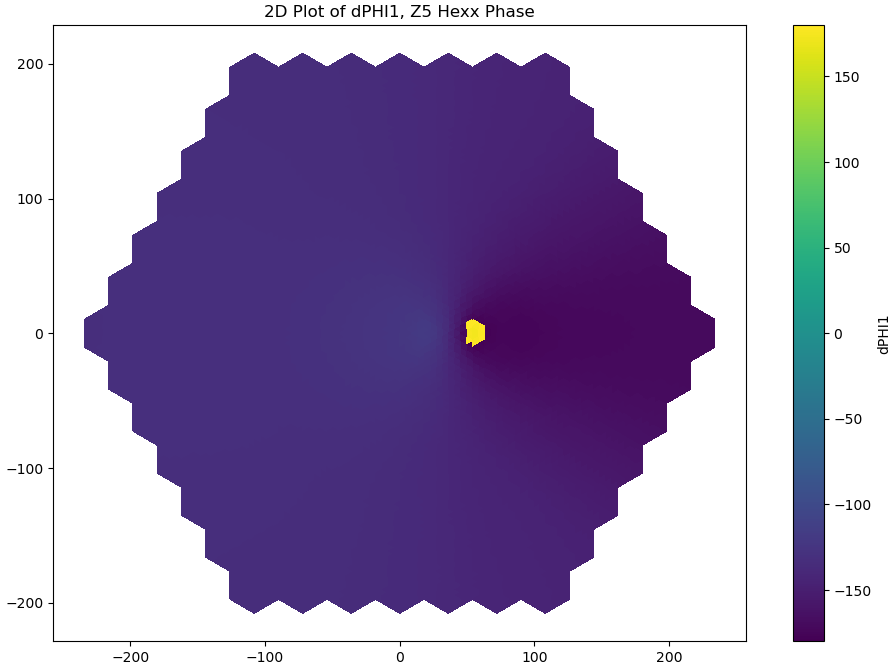
\includegraphics[width=\linewidth]{figures/OBJECTIVES3_TEST08_3DTriMG_HTTR_FAV_level3_NOISE_dPHI_phase_G1_Z5.png}
        \end{subfigure}
        \hfill
        \begin{subfigure}{.48\textwidth}
          \centering
          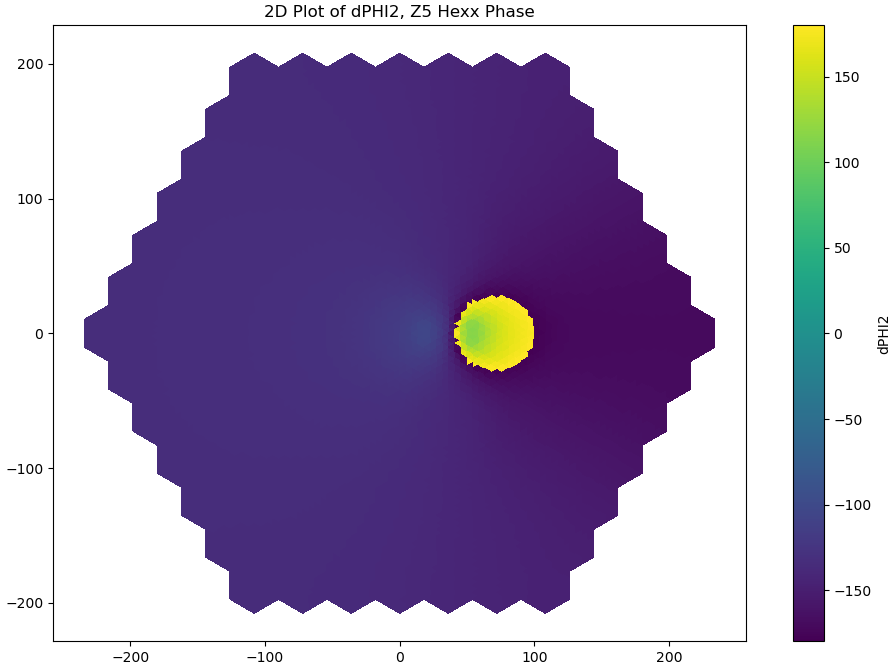
\includegraphics[width=\linewidth]{figures/OBJECTIVES3_TEST08_3DTriMG_HTTR_FAV_level3_NOISE_dPHI_phase_G2_Z5.png}
        \end{subfigure}
        \caption{Phase of the neutron noise for FAV in 3D HTTR at midplane ($Z = 5$)}
        \label{fig:3DHTTR_noise_FAV_results_phase}
\end{figure}

As seen in Figure \ref{fig:3DHTTR_noise_FAV_results_mag} and Figure \ref{fig:3DHTTR_noise_FAV_results_phase}, the neutron noise is more apparent in the thermal group and more dispersed in the fast group. This is a similar phenomenon compared to the FAV source in 2D HTTR. A similar opposing effect is expected in this case due to the out-of-phase neutron noise source model. Since the vibrating assembly is a fuel assembly, the opposing effect is not so apparent in the interfaces where the neighboring assembly is also a fuel assembly. This is expected since the difference between the macroscopic  cross-sections ($\Delta \Sigma_{a,g}$) is smaller at these interfaces. However, the opposing effect becomes more evident at the interfaces where the neighboring assembly is a reflector assembly. 

To further understand the driving force of neutron noise, we can split the neutron noise into its point kinetic component and its spatial component. Figures \ref{fig:3DHTTRFAV_noise_component_results1} and \ref{fig:3DHTTRFAV_noise_component_results2} show the point kinetic component and spatial component of the neutron noise in fast and thermal group with FAV source, taken at the centerline of the core ($y=0$) and midplane ($Z=5$).
\begin{figure}[H]
        \centering
        \begin{subfigure}{.48\textwidth}
          \centering
          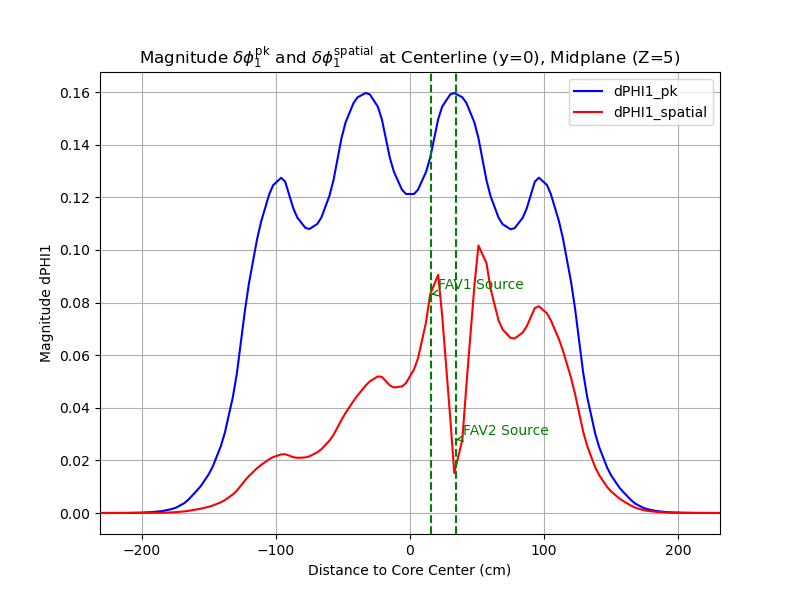
\includegraphics[width=\linewidth]{figures/Centerline_y0_OBJECTIVES3_TEST08_3DTriMG_HTTR_FAV_level3_dPHI_magnitude_G1.png}
        \end{subfigure}
        \hfill
        \begin{subfigure}{.48\textwidth}
          \centering
          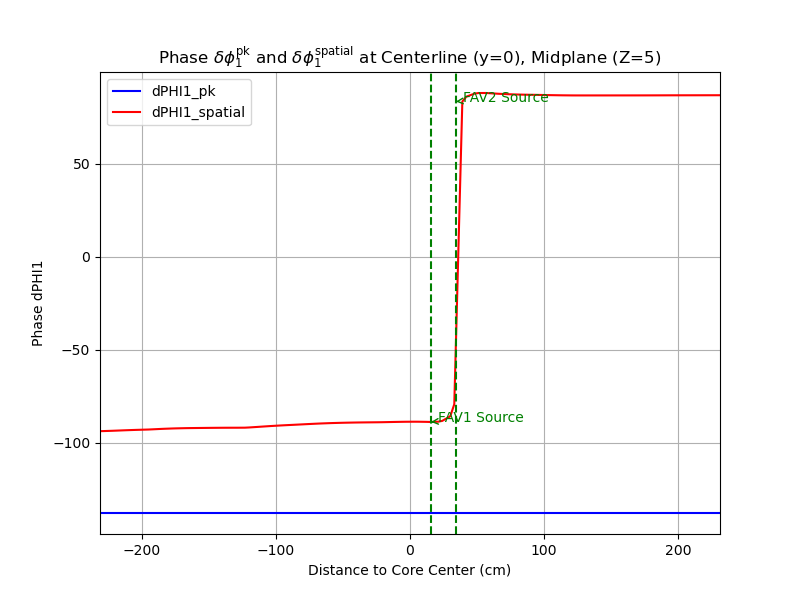
\includegraphics[width=\linewidth]{figures/Centerline_y0_OBJECTIVES3_TEST08_3DTriMG_HTTR_FAV_level3_dPHI_phase_G1.png}
        \end{subfigure}
        \caption{Magnitude (left) and phase (right) of the components of fast neutron noise for FAV in 3D HTTR at centerline ($y=0$), midplane ($z=5$)}
        \label{fig:3DHTTRFAV_noise_component_results1}
\end{figure}
\begin{figure}[H]
        \centering
        \begin{subfigure}{.48\textwidth}
          \centering
          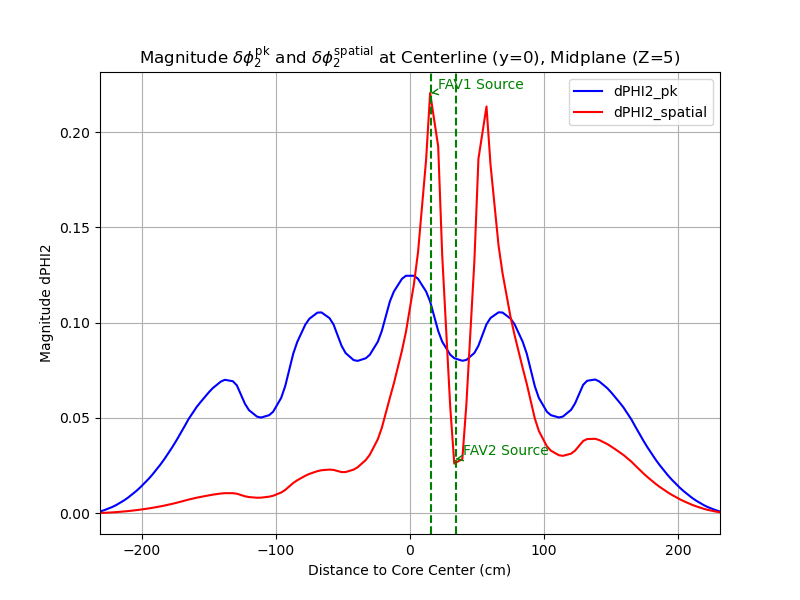
\includegraphics[width=\linewidth]{figures/Centerline_y0_OBJECTIVES3_TEST08_3DTriMG_HTTR_FAV_level3_dPHI_magnitude_G2.png}
        \end{subfigure}
        \hfill
        \begin{subfigure}{.48\textwidth}
          \centering
          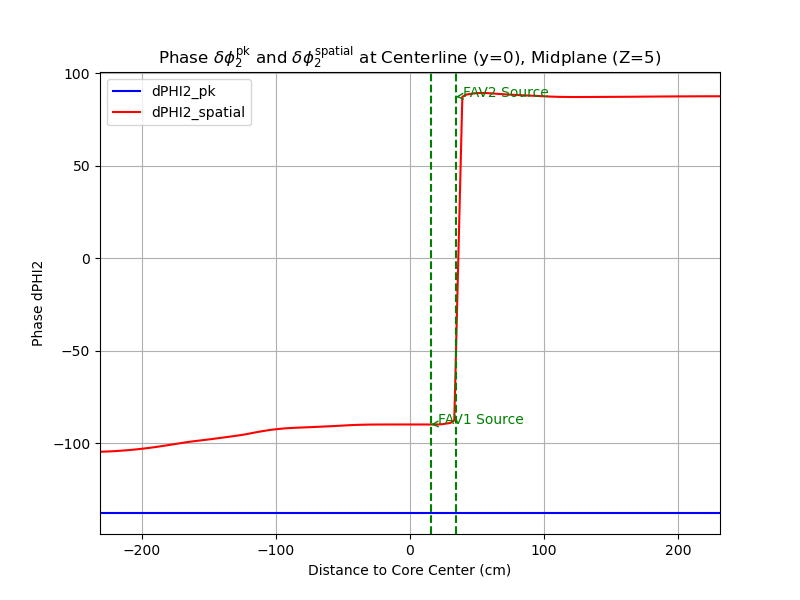
\includegraphics[width=\linewidth]{figures/Centerline_y0_OBJECTIVES3_TEST08_3DTriMG_HTTR_FAV_level3_dPHI_phase_G2.png}
        \end{subfigure}
        \caption{Magnitude (left) and phase (right) of the components of thermal neutron noise for FAV in 3D HTTR at centerline ($y=0$), midplane ($z=5$)}
        \label{fig:3DHTTRFAV_noise_component_results2}
\end{figure}

Comparing Figure \ref{fig:3DHTTRFAV_noise_component_results1} and Figure \ref{fig:3DHTTRFAV_noise_component_results2}, we see that the spatial component in the fast group has more influence than in the other cases. The point kinetic component remains dominant in this case, resulting in a more dispersed magnitude of neutron noise in the fast group. In the thermal group, we can see that the spatial component dominates the magnitude of the neutron noise. Similar to the 3D HTTR AVS case, the spatial component influences the phase delays similarly to the AVS source. Out-of-phase delays are more apparent compared to other cases. In general, we can see that the point kinetic component and the spatial component have different effects on the magnitude of neutron noise, while the phase of the neutron noise is mainly affected by the spatial component of the neutron noise. 

\section{Comparison of Noise Responses Between HTTR and LWR}

\subsection{2D Neutron Noise Responses}

For the comparison in 2D, the ZPRTF from 2D HTTR is compared with the ZPRTF from 2D C3 Benchmark, 2D BIBLIS Benchmark, and 2D VVER-400. The neutron noise simulation of 2D C3 Benchmark, 2D VVER-400 and 2D BIBLIS Benchmark will be shown in Appendix \ref{ch:appendixA}.

This comparison is done by performing 100 simulations for each 2D cases with variable frequencies, ranging from $10^{-4}$ Hz to $10^{4}$ Hz. The results of ZPRTF are shown in Figure \ref{fig:2DTransferFunction}.
\begin{figure}[H]
        \centering
        \begin{subfigure}{.48\textwidth}
          \centering
          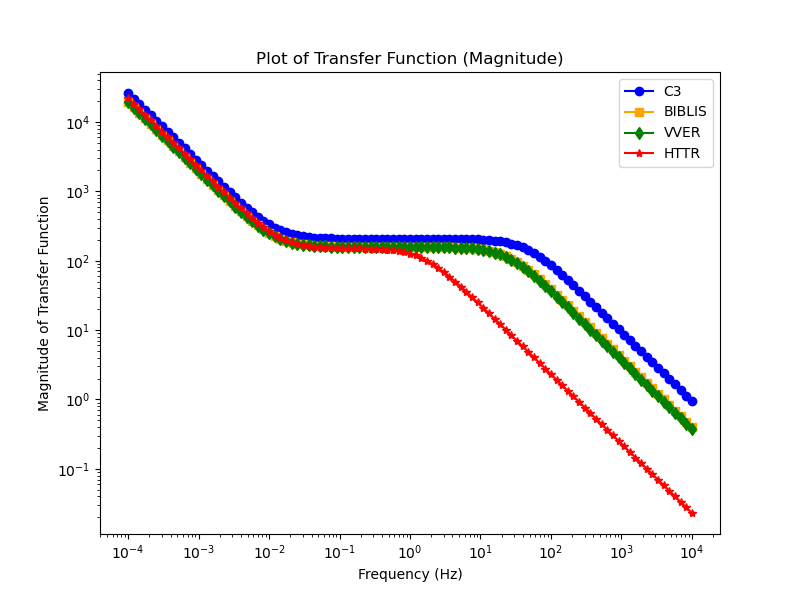
\includegraphics[width=\linewidth]{figures/Transfer_Function_2D_Comparison_Magnitude.png}
        \end{subfigure}
        \hfill
        \begin{subfigure}{.48\textwidth}
          \centering
          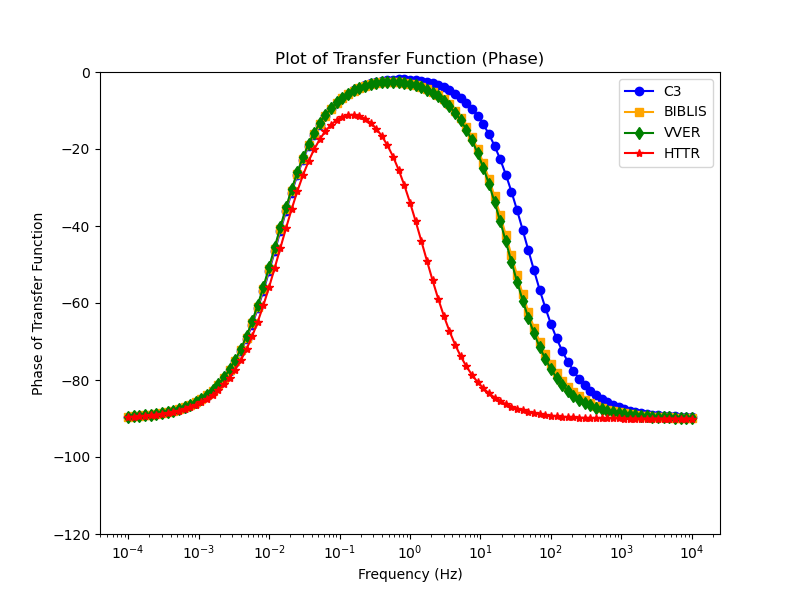
\includegraphics[width=\linewidth]{figures/Transfer_Function_2D_Comparison_Phase.png}
        \end{subfigure}
        \caption{Magnitude (left) and phase delay (right) of transfer function in 2D HTTR}
        \label{fig:2DTransferFunction}
\end{figure}

As seen in Figure \ref{fig:2DTransferFunction}, the ZPRTF of 2D HTTR generally follows the expected behavior of the ZPRTF. At lower and higher frequencies, the transfer function generally follows the $1/\omega$ behavior, which is expected in the ZPRTF. However, we can see that the 2D HTTR has a narrower plateau compared to other transfer functions. In the phase delay plot, we can see that the peak of 2D HTTR ZPRTF is further away from zero compared to other transfer functions. The HTTR ZPRTF deviates at around 1 Hz to 50 Hz. This means that within these frequencies, the spatial component of neutron noise in HTTR will have more significant effect compared to LWRs at the same range of frequencies.

\subsection{3D Neutron Noise Responses}

For the comparison in 3D, the ZPRTF from 3D HTTR is compared with the ZPRTF from 3D Westinghouse 4-loop PWR , 3D Langenbuch (LMW) Benchmark, and 3D VVER-400. The neutron noise simulation of 3D Westinghouse 4-loop PWR, 3D Langenbuch (LMW) Benchmark, and 3D VVER-400 will be shown in Appendix \ref{ch:appendixA}.

Similar to the 2D case, this comparison is done by performing 100 simulations for each 3D cases with variable frequencies, ranging from $10^{-4}$ Hz to $10^{4}$ Hz. The results of ZPRTF are shown in Figure \ref{fig:3DTransferFunction}.
\begin{figure}[H]
        \centering
        \begin{subfigure}{.48\textwidth}
          \centering
          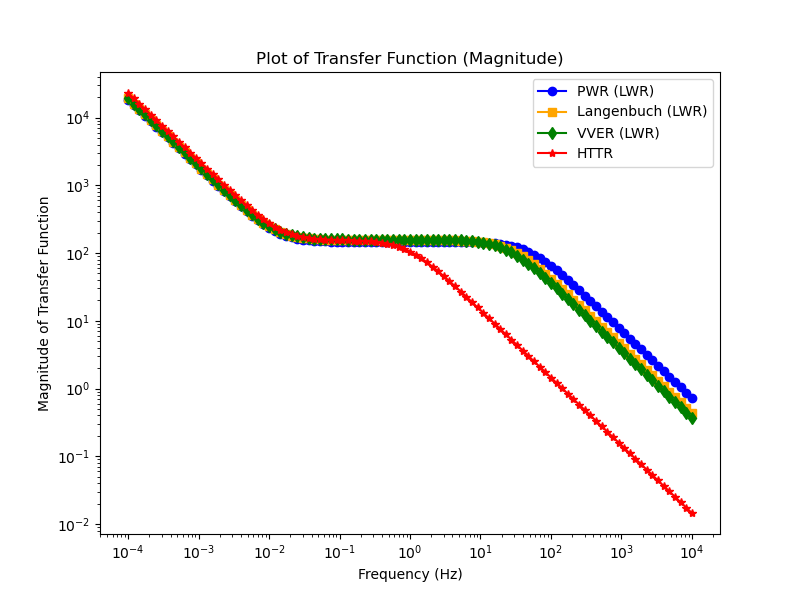
\includegraphics[width=\linewidth]{figures/Transfer_Function_3D_Comparison_Magnitude.png}
        \end{subfigure}
        \hfill
        \begin{subfigure}{.48\textwidth}
          \centering
          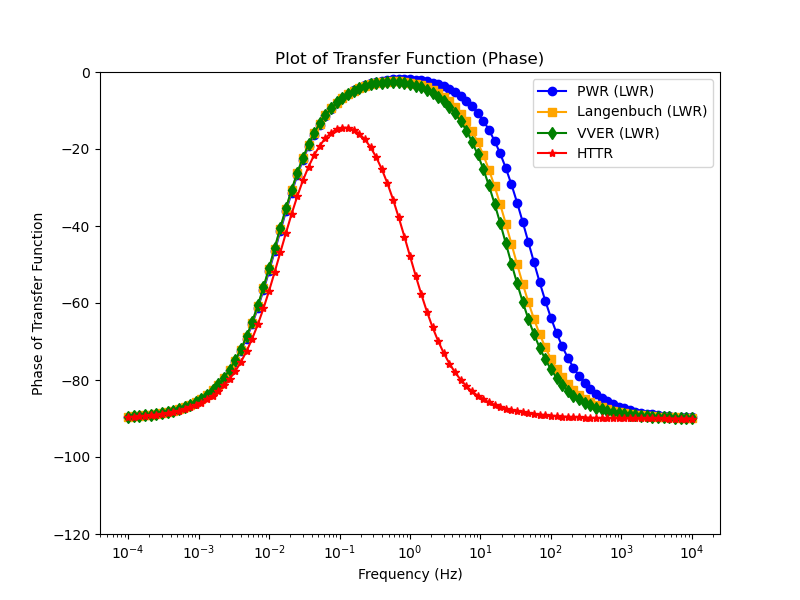
\includegraphics[width=\linewidth]{figures/Transfer_Function_3D_Comparison_Phase.png}
        \end{subfigure}
        \caption{Magnitude (left) and phase delay (right) of transfer function in 3D HTTR}
        \label{fig:3DTransferFunction}
\end{figure}

As seen in Figure \ref{fig:3DTransferFunction}, the ZPRTF of 3D HTTR generally follows the expected behavior of the ZPRTF, as expected. At lower and higher frequencies, the transfer function generally follows the $1/\omega$ behavior. Similar to the 2D HTTR case, we also see that the 3D HTTR has a shorter plateau compared to other transfer functions. In the phase delay plot, we can see that the peak of 3D HTTR ZPRTF is further away from zero compared to other transfer functions. The HTTR ZPRTF deviates at around 1 Hz to 50 Hz. Similar to the 2D HTTR case, this means that within these frequencies, the spatial component of neutron noise in HTTR will have more significant effect compared to LWRs at the same range of frequencies.

\section{Conclusion}

In this chapter, neutron noise simulations of 2D and 3D HTTR have been performed using two different noise sources for each geometry: the absorber of variable strength and the fuel assembly vibration.

For the absorber of variable strength source, both 2D and 3D HTTR simulations show that the neutron noise is more localized in the thermal group and more dispersed in the fast group. This is likely due to the larger mean free path of neutrons in the fast group. It is also observed that the point kinetic component of the neutron noise is more dominant than the spatial component of neutron noise. For the fuel assembly vibration case, a similar localized effect is observed in the thermal group. Additionally, the 2D and 3D HTTR FAV results show that the spatial component of the neutron noise has significant effect on the overall effect of neutron noise. This is more apparent when the neighboring assembly of the vibrating has a different characteristic (e.g., the neighboring assembly of the fuel assembly is a reflector assembly). Overall, the results show that the point kinetic component of neutron noise is more dominant than the spatial component in HTTR. This shows that the neutron noise is largely driven by the reactivity effect of the perturbation.

The ZPRTF of 2D and 3D HTTR was also compared with LWRs. The results show that HTTR generally follows the expected behavior of ZPRTF. The uniqueness of HTTR lies in the fact that it has a narrower plateau compared to LWRs. This means that at around 1 Hz to 50 Hz, the spatial component of neutron noise in HTTR will have more significant effect compared to LWRs. Overall, the simulations show that HTTR follows the expected behavior of neutron noise. Thus, neutron noise analysis can be used to detect anomalies in HTTR.

\chapter{The Neutron Noise Sources Unfolding Methods}
\label{ch:unfolding_methods}

To perform anomaly detection on the core, we need to apply neutron noise unfolding methods. Unfolding methods in this case are used to determine the parameters of neutron noise sources, including their magnitude, frequency, energy, and location. Neutron noise unfolding methods have been developed in the past and verified for the absorber of variable strength-type noise source, mainly light water reactor cores \cite{karlssonLocalizationChannelInstability1999, demaziereDevelopmentNonintrusiveMethod2002, demaziereIdentificationLocalizationAbsorbers2005}. The methods are the inversion method, zoning method, and scanning method. The methods rely on the use of Green’s function, which can be pre-calculated without the need to know the true neutron noise source in the core.

This chapter introduces two novel neutron noise unfolding methods based on Green’s function. These methods are called the brute force method and the greedy method. One more method, called the backward elimination method, has also been developed. However, this method is not reliable for multiple noise sources. The details for the backward elimination method are available in Appendix \ref{ch:appendixB}. For the sake of completeness, this chapter also outlines the derivation of existing neutron noise unfolding methods. These methods are used as a comparison of the new methods for HTTR core application.

The structure of this chapter is as follows. First, we will provide the derivation of Green’s function for neutron noise unfolding methods. In here, we will provide the derivation of the neutron noise as a function of the Green’s function. Second, we will provide the existing neutron noise unfolding methods and their derivations. Third, we will introduce novel neutron noise unfolding methods, their derivation and computational algorithm. Fourth, we will apply all the neutron noise unfolding methods to the 2D and 3D HTTR core. In these cases, the AVS-type noise source is used for practicality. Finally, we will provide the limitations of the novel methods and the conclusion of the chapter.

\section{Green's Function for Neutron Noise Unfolding}

Neutron noise source unfolding is a method used to identify the type of noise source and locate the position at which perturbations occur. Generally, the noise source unfolding method depends on Green’s function. Hence, determining Green’s function from the neutron noise equation is necessary \cite{demaziereIdentificationLocalizationAbsorbers2005}. We begin with the definition of the neutron noise equation in operator form.
\begin{equation}
    B(\textbf{r}) \delta \phi(\textbf{r},\omega) = S(\textbf{r},\omega)
\end{equation}
where $B(\textbf{r})$ is the Boltzmann-like operator for the complex neutron noise equation and $S(\textbf{r},\omega)$ is the neutron noise source term. Since neutron noise can be described as a localized (impulse-like) perturbation, we define Green's function of $B(\textbf{r})$ to be the unique solution of Eq. \ref{eq:Green_function1}.
\begin{equation}\label{eq:Green_function1} 
    B(\textbf{r}) G(\textbf{r}, \textbf{r}_p,\omega) = \delta(\textbf{r}-\textbf{r}_p)
\end{equation}
Then, we can define,
\begin{equation}\label{eq:greens_function}
    \delta \phi(\textbf{r}, \omega) = \int_{V_p} G(\textbf{r}, \textbf{r}_p,\omega) S(\textbf{r}_p,\omega) dV_p
\end{equation}
where
\begin{itemize}
    \item[] $\delta \phi(\textbf{r}, \omega) $ = Neutron noise,
    \item[] $G(\textbf{r}, \textbf{r}_p,\omega)$ = Green's function matrix,
    \item[] $S(\textbf{r}_p,\omega)$ = Neutron noise sources to be unfolded.
\end{itemize}

In finite mesh, Eq. \ref{eq:greens_function} can be discretized and be written as matrix-vector multiplication:
\begin{equation}
    \delta \phi(\textbf{r}, \omega) = G(\textbf{r}, \textbf{r}_p,\omega) S(\textbf{r}_p,\omega)
\end{equation}
Therefore, the noise source can be determined by inverting the Green’s function such that:
\begin{equation}\label{eq:source_initial}
    S(\textbf{r}_p,\omega) = G^{-1}(\textbf{r}, \textbf{r}_p,\omega) \delta \phi(\textbf{r}, \omega)
\end{equation}

Suppose the neutron noise is known at every location in the core. In that case, it is trivial to obtain the neutron noise source information, including the magnitude and location, by inverting the Green’s function matrix. However, this is not the case due to the limitation of detector locations. This means that Eq. \ref{eq:source_initial} should be written as:
\begin{equation}\label{eq:source_meas}
    S(\textbf{r}_p,\omega) = G^{-1}(\textbf{r}_{\text{meas}}, \textbf{r}_p,\omega) \delta \phi(\textbf{r}_{\text{meas}}, \omega)
\end{equation}
where $\delta \phi(\textbf{r}_{\text{meas}}, \omega)$ means that the neutron noise is known at detector locations (measured) and zero otherwise. This creates a non-square matrix for the Green’s function, which makes it ill-posed to invert. This is the main challenge of neutron noise unfolding methods.

\section{Existing Neutron Noise Unfolding Methods}

\subsection{Inversion Method}

Inversion method is proposed by \cite{demaziereIdentificationLocalizationAbsorbers2005} to unfold the neutron noise sources by interpolating the detector readings to match the vector size $\delta \phi (\textbf{r}, \omega)$. The study assumes that the detector is sensitive to thermal neutron and the noise source is known to be a perturbation of thermal absorption cross-section \cite{demaziereIdentificationLocalizationAbsorbers2005}. The interpolated neutron noise $\delta \phi (\textbf{r}_{\text{interp}}, \omega)$ can be written as follows:
\begin{equation}
    \begin{aligned}
        \delta \phi (\textbf{r}_{\text{interp}}, \omega) &= \overline{\overline{T}} \delta \phi (\textbf{r}, \omega) \\
        &= \overline{\overline{T}} G(\textbf{r}, \textbf{r}_p,\omega) S(\textbf{r}_p,\omega) \\
        &= G(\textbf{r}_{\text{interp}}, \textbf{r}_p,\omega) S(\textbf{r}_p,\omega)
    \end{aligned}
\end{equation}
Therefore, the neutron noise source is written as:
\begin{equation}
    S(\textbf{r}_p,\omega) = G^{-1}(\textbf{r}_{\text{interp}}, \textbf{r}_p,\omega) \delta \phi (\textbf{r}_{\text{interp}}, \omega)
\end{equation}
where $\overline{\overline{T}}$ is a matrix that represents the interpolation process \cite{demaziereIdentificationLocalizationAbsorbers2005}. In this case, $G^{-1}(\textbf{r}_{\text{interp}}, \textbf{r}_p,\omega)$ has size $(\text{group} \times N), (\text{group} \times  N)$, $\delta \phi (\textbf{r}_{\text{interp}}, \omega)$ has size $\text{group} \times N$, and $S(\textbf{r}_p,\omega)$ has size $\text{group} \times N$. This means that not only the $\delta \phi (\textbf{r}, \omega)$ that needs to be interpolated, but also $G(\textbf{r}, \textbf{r}_p,\omega)$ that needs to be interpolated.

The pseudo algorithm of the inversion method is described in Algorithm~\ref{alg:inversion}.
\begin{algorithm}[H]
\caption{: Inversion Method}
\label{alg:inversion}
\begin{algorithmic}[1]
\Require Measured neutron noise $\delta \phi(\textbf{r}_{\text{meas}}, \omega)$, Green’s function matrix $G(\textbf{r}, \textbf{r}_p,\omega)$, energy groups $g$, position mesh $n$
\Ensure Reconstructed neutron noise $\delta \phi_{\text{INVERT}}(\textbf{r}, \omega)$, unfolded source $S_{\text{INVERT}}(\textbf{r}, \omega)$
\For{each group $g$} \Comment{\textbf{Interpolate $\delta \phi_{\text{meas}}$}}
    \State Collect geometry data
    \State Interpolate missing values via RBF $\rightarrow \delta \phi_{\text{INVERT}}(\textbf{r}, \omega)$
\EndFor
\For{each group $g$ and position $n$} \Comment{\textbf{Interpolate $G(\textbf{r}_{\text{meas}}, \textbf{r}_p,\omega)$}}
    \State Interpolate missing columns of $G$ $\rightarrow G(\textbf{r}_{\text{interp}}, \textbf{r}_p,\omega)$
\EndFor
\State Compute $G^{\dagger}(\textbf{r}_{\text{interp}}, \textbf{r}_p,\omega) =$ pseudo-inverse of interpolated $G$ \Comment{\textbf{Invert System}}
\State Compute unfolded sources $S_{\text{INVERT}}(\textbf{r}_p,\omega) = G^{\dagger}(\textbf{r}_{\text{interp}}, \textbf{r}_p,\omega) \delta \phi_{\text{INVERT}}(\textbf{r}, \omega)$
\State \textbf{Postprocess}: $S_{\text{INVERT}}(\textbf{r},\omega)$ file, $\delta \phi_{\text{INVERT}}(\textbf{r}, \omega)$ file, plots. 
\end{algorithmic}
\end{algorithm}

This method is able to reconstruct the noise source. However, this inversion method might have some problems in the boundaries because the interpolated thermal flux perturbation is forced to be equal to zero outside the reflector nodes. Even though the reconstruction at the boundaries produced poor approximation, the overall process still provides promising results. The result of this method is highly dependent on the interpolation process.

\subsection{Zoning Method}

The zoning method is an extension of the inversion method. The difference between the two lies in using zones in the zoning method instead of interpolation. In the zoning method, the reactor is divided into several zones, $Z_k$. Each zone has the number of detectors that is identical to the number of fuel assemblies in the zone. In this method, the flux perturbation can be written as \cite{demaziereIdentificationLocalizationAbsorbers2005}:
\begin{equation}
    \delta \phi (\textbf{r}_{\text{meas}}, \omega) = \sum_k G(\textbf{r}_{\text{meas}}, \textbf{r}_{Z_k},\omega) S(\textbf{r}_{Z_k},\omega)
\end{equation}
Since the number of detectors and the fuel assembly in the zone is identical, the Green’s function matrix $G(\textbf{r}_{\text{meas}}, \textbf{r}_{Z_k},\omega)$ for each zone is a square matrix. This means that interpolation of the Green’s function is no longer necessary.

If the fuel assemblies represented in the zone $Z_k$ are set not to be close to each other, the response of the thermal flux detector will be unique to each other. Having the fuel assemblies belonging to a given zone $Z_k$ evenly distributed throughout the core is an easy and practical way to achieve such a goal.

Then, by inverting one of the matrices $G(\textbf{r}_{\text{meas}}, \textbf{r}_{Z_k},\omega)$ for zone $Z_l$, one can obtain:
\begin{equation}\label{eq:zoning_start}
    G^{-1}(\textbf{r}_{\text{meas}}, \textbf{r}_{Z_l},\omega) \delta \phi (\textbf{r}_{\text{meas}}, \omega) = G^{-1}(\textbf{r}_{\text{meas}}, \textbf{r}_{Z_l},\omega) \biggl( \sum_{k \neq l} G(\textbf{r}_{\text{meas}}, \textbf{r}_{Z_k},\omega) S(\textbf{r}_{Z_k},\omega) \biggr) + S(\textbf{r}_{Z_l},\omega)
\end{equation}
Moving forward, we will assume that the noise source is located at $Z_s$, which might be at one of the $Z_k$ or at $Z_l$. We have two possible cases:
\begin{enumerate}
    \item If the noise source is located at the zone $Z_l=Z_s$, then one can write:
    \begin{equation}
        G^{-1}(\textbf{r}_{\text{meas}}, \textbf{r}_{Z_l},\omega) \delta \phi (\textbf{r}_{\text{meas}}, \omega) =  S(\textbf{r}_{Z_l},\omega)
    \end{equation}
    In this case, $S(\textbf{r}_{Z_l},\omega)= S(\textbf{r}_{Z_s},\omega)$ is the “true” noise source vector. The noise source vector would have a distinct peak from any other zone, indicating that the noise source is in the zone $Z_l$.
    \item If the inversion is done to the matrix corresponding to zone $Z_l \neq Z_s$ (contains no noise source), then Eq. \ref{eq:zoning_start} becomes:
    \begin{equation}
        G^{-1}(\textbf{r}_{\text{meas}}, \textbf{r}_{Z_l},\omega) \delta \phi (\textbf{r}_{\text{meas}}, \omega) = G^{-1}(\textbf{r}_{\text{meas}}, \textbf{r}_{Z_l},\omega) G(\textbf{r}_{\text{meas}}, \textbf{r}_{Z_k},\omega) S(\textbf{r}_{Z_k},\omega)
    \end{equation}
    This means that the zone $Z_l$ does not contain the noise source vector. The right-hand side of the equation will be relatively flat and no peak will be visible \cite{demaziereIdentificationLocalizationAbsorbers2005}.
\end{enumerate}

To simplify the analysis, we can perform the following calculation.
\begin{equation}
    G^{-1}(\textbf{r}_{\text{meas}}, \textbf{r}_{Z_l},\omega) \delta \phi (\textbf{r}_{\text{meas}}, \omega) =  S_{\text{fict}}(\textbf{r}_{Z_l},\omega)
\end{equation}
where $Z_l \in Z_k$. This calculation is done for every zone, which results in $k$ number of $S_{\text{fict}}(\textbf{r}_{Z_l},\omega)$. For each $S_{\text{fict}}(\textbf{r}_{Z_l},\omega)$, it should return to one of the both cases. If the zone $Z_l$ If the signal contains a noise source, then one of the vector elements should be significantly higher than the others. On the other hand, if a zone $Z_l$ does not contain a noise source, the elements of $S_{\text{fict}}(\textbf{r}_{Z_l},\omega)$ would not be different from each other.

The pseudo algorithm of the zoning method is described in Algorithm~\ref{alg:zoning}.
\begin{algorithm}[H]
\caption{: Zoning Method}
\label{alg:zoning}
\begin{algorithmic}[1]
\Require Measured neutron noise $\delta \phi(\textbf{r}_{\text{meas}}, \omega)$, Green’s function matrix $G(\textbf{r}, \textbf{r}_p,\omega)$, energy groups $g$, position mesh $n$, zone map
\Ensure Unfolded source $S_{\text{ZONE}}(\textbf{r}, \omega)$
\State Compute zone sizes (length of each zone) \Comment{\textbf{Zone mapping}}
\State For each zone $Z_l$, extract a subset of $\delta \phi(\textbf{r}_{\text{meas}}, \omega)$ values \Comment{\textbf{Divide $\delta \phi(\textbf{r}_{\text{meas}}, \omega)$ into zones}}
\State Save zone-wise $\delta \phi(\textbf{r}_{\text{meas}, Z_l}, \omega)$
\For{each zone $Z_l$} \Comment{\textbf{Divide $G(\textbf{r}_{\text{meas}}, \textbf{r}_p,\omega)$ into zones}}
    \State Extract $G(\textbf{r}_{\text{meas}}, \textbf{r}_{Z_l},\omega)$
\EndFor
\For{each zone $Z_l$} \Comment{\textbf{Solve zone systems}}
    \State Extract zone vector $\delta \phi(\textbf{r}_{\text{meas}, Z_l}, \omega)$
    \State Compute pseudo-inverse of $G(\textbf{r}_{\text{meas}}, \textbf{r}_{Z_l},\omega)$
    \State Solve $S_{\text{ZONE}}(\textbf{r}_{Z_l},\omega) = G^{\dagger}(\textbf{r}_{\text{meas}}, \textbf{r}_{Z_l},\omega) \delta \phi(\textbf{r}_{\text{meas}, Z_l}, \omega)$
    \State Map results back into global $S_{\text{ZONE}}(\textbf{r},\omega)$
\EndFor
\State \textbf{Postprocess:} $S_\text{ZONE}(\textbf{r},\omega)$ file, plots. 
\end{algorithmic}
\end{algorithm}

The zoning method generally improves the accuracy of the noise unfolding. Poor performance was observed when the noise source was located near the boundary of several detectors. In this location, the detector responses will not be unique to each other, making the Green’s function inaccurate \cite{demaziereIdentificationLocalizationAbsorbers2005}.

\subsection{Scanning Method}

The third method is the scanning method. This method compares the perturbations detected by the detector with the calculated response for all possible locations of the noise source within the system. The noise source is accurately identified when the calculated neutron noise matches the measured neutron noise \cite{demaziereIdentificationLocalizationAbsorbers2005}. This method was developed by \cite{karlssonLocalizationChannelInstability1999} and extended by \cite{demaziereDevelopmentNoisebasedMethod2002}. Both investigations successfully determined the location of the unseated fuel assembly in the Swedish Forsmark-1 BWR. Both use Green’s function as the means to compare detector readings.
This method starts with the definition of neutron noise at a given location $\textbf{r}$ induced by a noise source located at the location $\textbf{r}_p$ as follows:
\begin{equation}\label{eq:scan_start}
    \delta \phi (\textbf{r}_{i}, \omega) = G(\textbf{r}_{i}, \textbf{r}_{p,j},\omega) S(\textbf{r}_{p,j},\omega)
\end{equation}
Using Eq. \ref{eq:scan_start} to compare with the detector reading will be difficult since the location and strength of the noise are unknown. If one has access to two detectors at locations A and B, the ratio between the neutron noise at these two locations can be used to eliminate the noise source strength:
\begin{equation}
    \frac{\delta \phi (\textbf{r}_{A}, \omega)}{\delta \phi (\textbf{r}_{B}, \omega)} = \frac{G(\textbf{r}_{A}, \textbf{r}_{p},\omega)}{G(\textbf{r}_{B}, \textbf{r}_{p},\omega)}
\end{equation}
Then, the scanning algorithm consists of minimizing the following:
\begin{equation}\label{eq:scan_min}
    \Delta(\textbf{r}) = \sum_{A,B} \biggl| \frac{\delta \phi (\textbf{r}_{A}, \omega)}{\delta \phi (\textbf{r}_{B}, \omega)} - \frac{G(\textbf{r}_{A}, \textbf{r}_{p},\omega)}{G(\textbf{r}_{B}, \textbf{r}_{p},\omega)} \biggr|
\end{equation}

Eq. \ref{eq:scan_min} implies that the summation is done for all detector pairs for all locations $r$. If there exist $n$ number of detectors in the reactor, thus the number of detector pairs is as follows:
\begin{equation}
    N_{\text{detector pair}} = \frac{n \times (n+1)}{2}
\end{equation}

The location at which the minimum value of $\Delta(\textbf{r})$ is found indicates the location of the noise source. The magnitude of the noise source can be calculated as follows:
\begin{equation} \label{eq:scan_source}
    S(\textbf{r}_{p},\omega) = \frac{\delta \phi (\textbf{r}_{m}, \omega)}{G(\textbf{r}_{m}, \textbf{r}_{p},\omega)}
\end{equation}
for any detector m.

The pseudo algorithm of the scanning method is described in Algorithm~\ref{alg:scanning}.
\begin{algorithm}[H]
\caption{: Scanning Method}
\label{alg:scanning}
\begin{algorithmic}[1]
\Require Measured neutron noise $\delta \phi(\textbf{r}_{\text{meas}}, \omega)$, Green’s function matrix $G(\textbf{r}, \textbf{r}_p,\omega)$, energy groups $g$, position mesh $n$
\Ensure Unfolded source $S_{\text{SCAN}}(\textbf{r}, \omega)$
\State Generate all detector pairs $(A,B) \in \mathcal{P}$
\State Initialize $\Delta(\textbf{r})$ \Comment{\textbf{Calculate $\Delta(\textbf{r})$}}
\For{each energy group $g = 1 \to group$}
    \For{each candidate source position $n$}
        \State Initialize $\Delta(g,n) \gets 0$
        \For{each detector pair $(A,B) \in \mathcal{P}$}
            \State Compute neutron noise ratio $\frac{\delta \phi (\textbf{r}_{A}, \omega)}{\delta \phi (\textbf{r}_{B}, \omega)}$
            \State Compute Green's function ratio $\frac{G(\textbf{r}_{A}, \textbf{r}_{p},\omega)}{G(\textbf{r}_{B}, \textbf{r}_{p},\omega)}$ for position $n$
            \State Update mismatch: $\Delta_{AB}(g,n) \mathrel{+}= \biggl| \frac{\delta \phi (\textbf{r}_{A}, \omega)}{\delta \phi (\textbf{r}_{B}, \omega)} - \frac{G(\textbf{r}_{A}, \textbf{r}_{p},\omega)}{G(\textbf{r}_{B}, \textbf{r}_{p},\omega)} \biggr|$
        \EndFor
        \State Store $\Delta_{AB}(g,n) \rightarrow \Delta(\textbf{r})$
    \EndFor
\EndFor

\State Find global minimum: 
\[
\textbf{r}_\text{min} = \arg\min_{\textbf{r}} \Delta(\textbf{r})
\]

\State Compute unfolding weight:
\[
W = \frac{\delta \phi (\textbf{r}_\text{min}, \omega)}{G(\textbf{r}_\text{min}, \textbf{r}_{p},\omega)}
\]
\State Initialize $S_{\text{SCAN}}(\textbf{r}, \omega)$ \Comment{\textbf{Calculate $S_{\text{SCAN}}(\textbf{r}, \omega)$}}
\State Assign $S_{\text{SCAN}}(\textbf{r}_\text{min}, \omega) \gets W$
\State \textbf{Postprocess:} $S_{\text{SCAN}}(\textbf{r}, \omega)$ file, plots. 
\end{algorithmic}
\end{algorithm}

The results from \cite{demaziereIdentificationLocalizationAbsorbers2005} show that the scanning algorithm was able to locate any noise source correctly, provided there is no background. The drawback of this method is that it requires more computational power to compare every possible location of the noise source with every combination of detectors used for the evaluation.

\section{Novel Neutron Noise Unfolding Methods}

\subsection{General Overview}

Considering the limitations of the existing methods, improvement in the generalization of the neutron noise unfolding method is desirable. This means that the methods should be able to unfold multiple neutron noise sources simultaneously. In this dissertation, three new neutron noise unfolding methods have been developed. The two new methods are described in the following section. The third method, the backward elimination method, will be described in Appendix \ref{ch:appendixB} since it is not reliable for multiple sources. These methods are based on the Green’s function matrix in Eq. \ref{eq:greens_function}. For a finite mesh, we can discretize Eq. \ref{eq:greens_function} as follows:
\begin{equation}\label{eq:greens_function2}
    \begin{aligned}
        \delta \phi(\textbf{r}, \omega) &= \int_{V_p} G(\textbf{r}, \textbf{r}_p,\omega) S(\textbf{r}_p,\omega) dV_p \\
        &= \sum_{\textbf{r}_p} G(\textbf{r}, \textbf{r}_p,\omega) S(\textbf{r}_p,\omega)
    \end{aligned}
\end{equation}
Since the $G(\textbf{r}, \textbf{r}_p,\omega)$ is given, then the neutron noise $\delta \phi(\textbf{r}, \omega)$ is the sum of combination of Green's function with coefficient $S(\textbf{r}_p,\omega)$. This means that the problem is finding the correct combination of Green’s function and the noise source that reconstructs the neutron noise. The noise source can be calculated using the Least Square method.

It should be noted that, computationally, Equation  \ref{eq:greens_function2} is applicable to unfold both AVS and FAV sources. This is because both AVS and FAV sources are computationally modeled as perturbation of cross sections at the mesh of interest. The AVS sources are defined as perturbation at a point in a mesh, while the FAV sources are defined as perturbation at the mesh boundaries. In a discretized equation, FAV sources are the same as multiple AVS sources at the boundaries.

\subsection{Brute Force Method}

Given Eq. \ref{eq:greens_function2} and the fact that neutron noise source is an impulse-like perturbation of the cross sections, The neutron noise source should only be nonzero at the location of the perturbation and zero otherwise. Therefore, there should be a combination of Green's function and its coefficient that would lead to the correct reconstructed neutron noise.

The brute force method, as the name suggests, solves every combination of Green’s functions until it finds a correct combination that reduces the residual norm between the Green’s function combination and the measured neutron noise to a specified tolerance. The residual norm tolerance was set to $10^{-10}$, which corresponds to the residual norm of the solution brute force. For every loop of Green’s function combination, the method solves for the coefficient of each combination ($S(\textbf{r}_p,\omega)$) and the residual. 

The flow diagram of the method is described in Figure \ref{fig:brute_force}.
\begin{figure}[H]
        \centering
        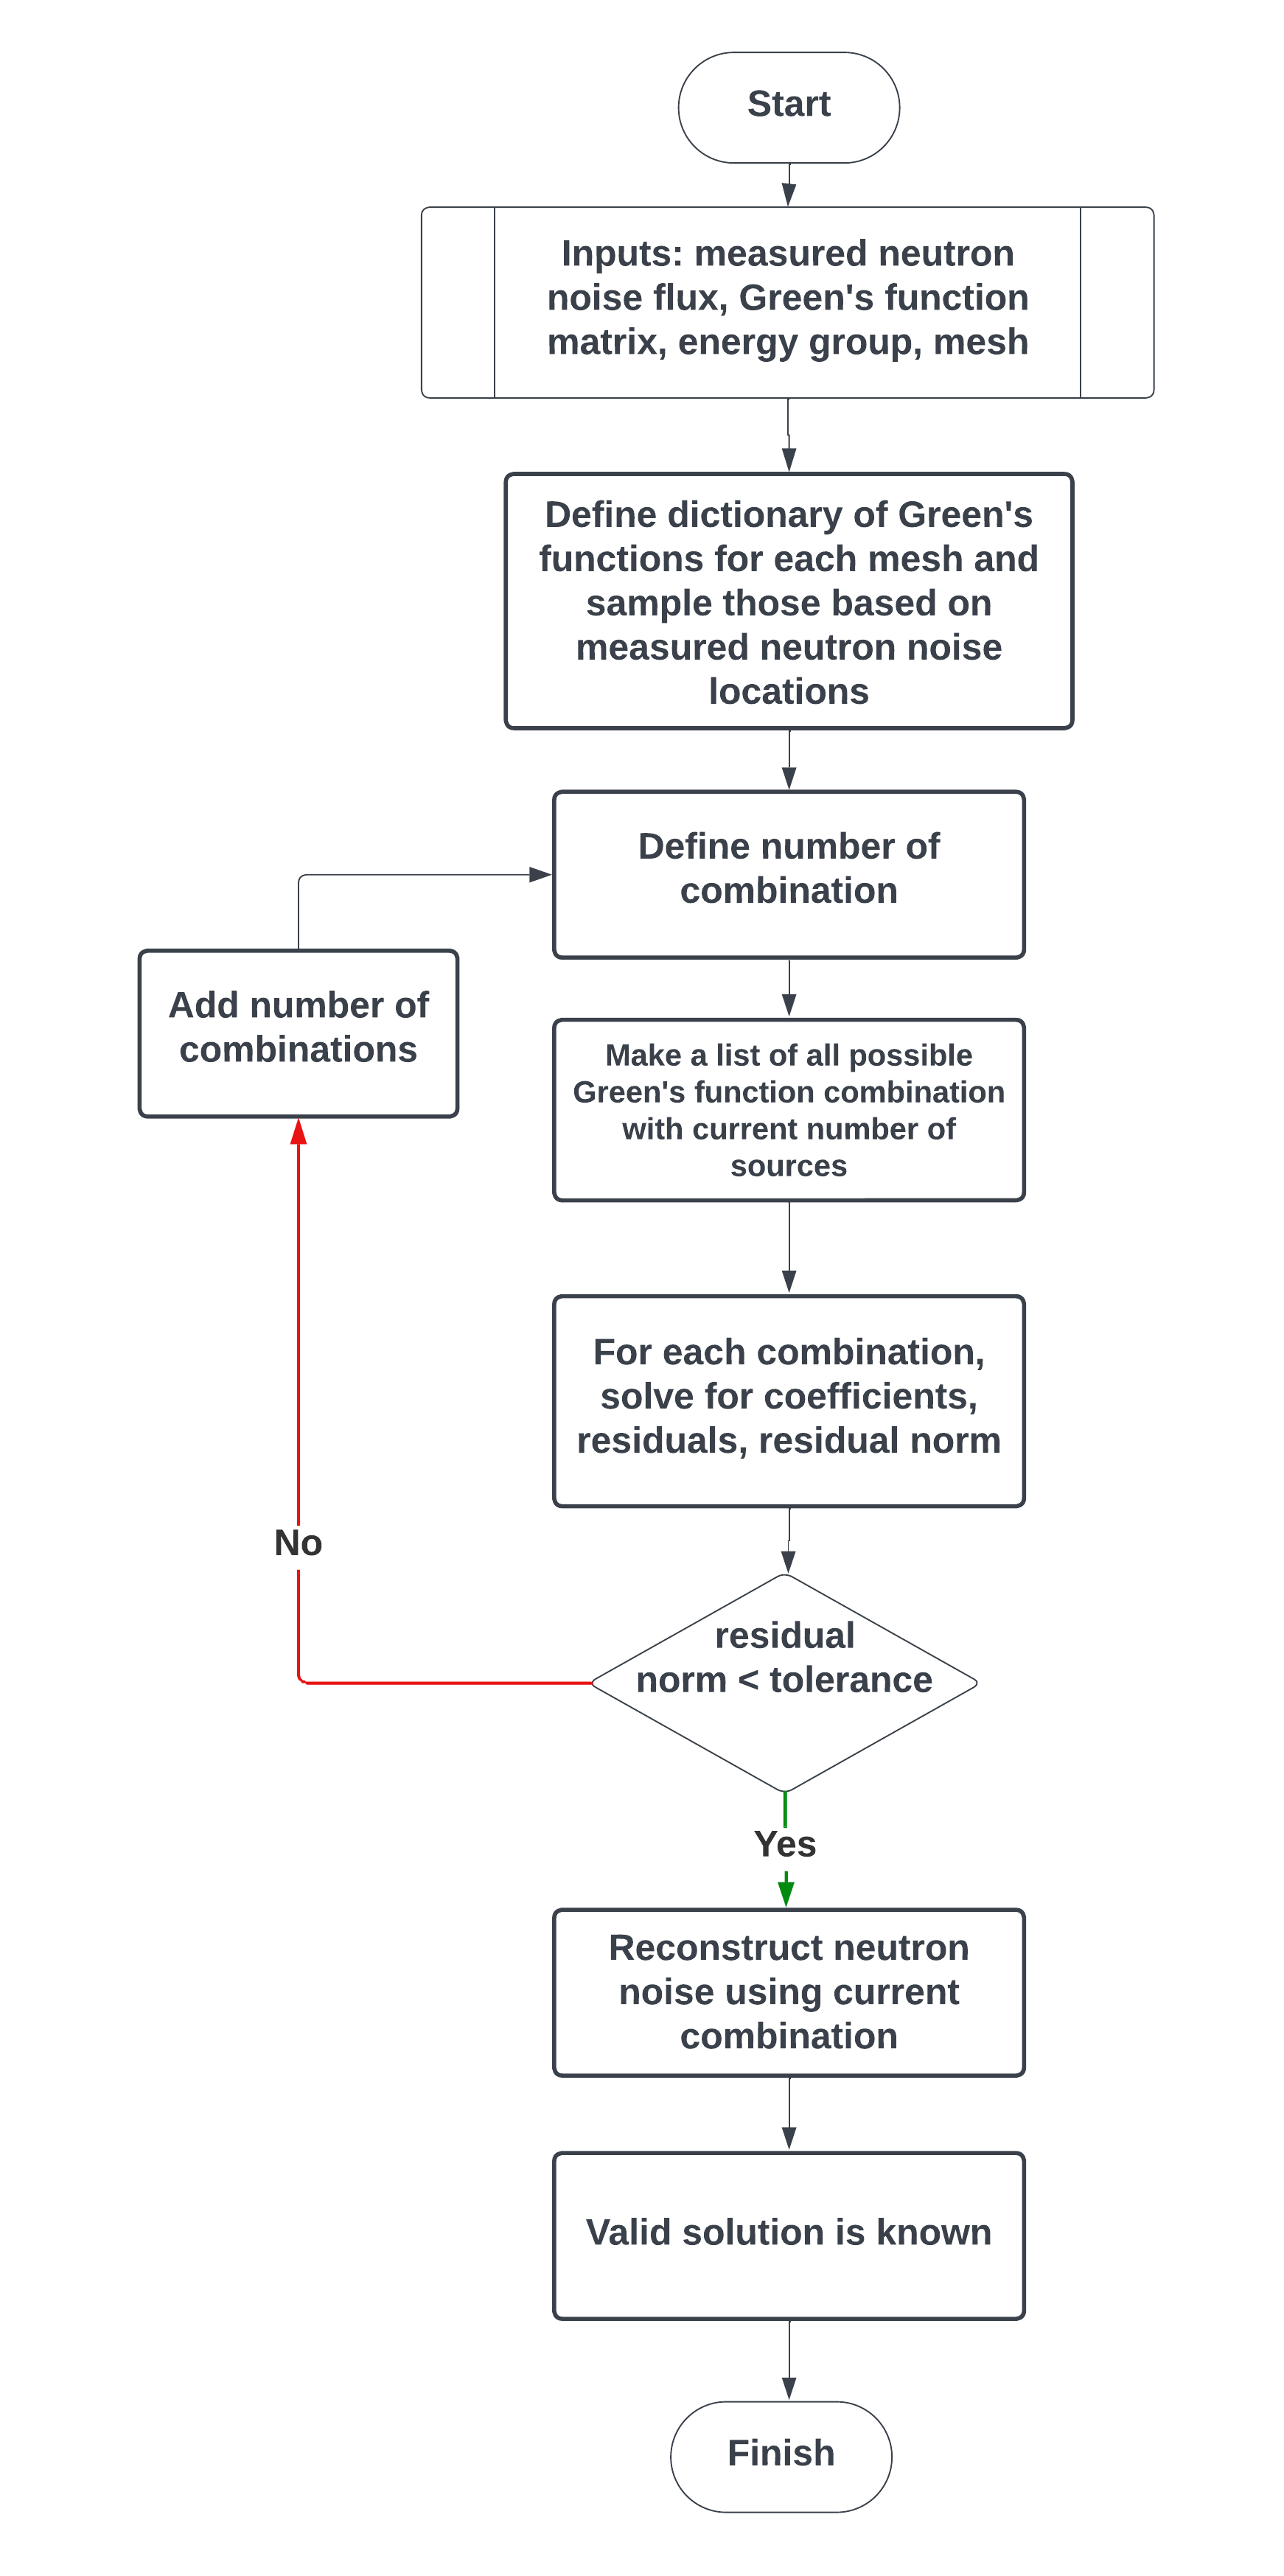
\includegraphics[width=0.6\textwidth]{figures/Brute Force Method.png}
        \caption{Flow diagram of brute force method}
        \label{fig:brute_force}
\end{figure}

The pseudo algorithm of the brute force method is described in Algorithm~\ref{alg:brute_force}.
\begin{algorithm}[H]
\caption{: Brute Force Method}
\label{alg:brute_force}
\begin{algorithmic}[1]
\Require Measured neutron noise $\delta \phi(\textbf{r}_{\text{meas}}, \omega)$, Green’s function matrix $G(\textbf{r}, \textbf{r}_p,\omega)$, energy groups $g$, mesh $N$
\Ensure reconstructed neutron noise $\delta \phi_{\text{BRUTE}}(\textbf{r}, \omega)$, unfolded source $S_{\text{BRUTE}}(\textbf{r}, \omega)$
\For{each group $g$} \Comment{\textbf{Construct Green’s function dictionary}}
    \For{each node $n$}
        \State Store columns of $G(\textbf{r}, \textbf{r}_p,\omega)$ in dictionary
    \EndFor
\EndFor
\State Sample columns only at measured (non-zero) indices

\For{$k = 1$ to total number of atoms} \Comment{\textbf{Brute-force search over subsets of atoms}}
    \State Calculate of subset of atoms of size $k$
    \ForAll{subsets of size $k$}
        \State Form matrix $A$ from selected atoms
        \State Solve least squares: $\mathbf{c} = \arg\min || \delta \phi(\textbf{r}_{\text{meas}}, \omega) - A \mathbf{c}||$
        \State Compute residual $r = ||\delta \phi(\textbf{r}_{\text{meas}}, \omega) - A \mathbf{c}||$
        \If{$r < \text{tolerance}$}
            \State Store valid $G_{g,n}$ solution
            \State Break all loops
        \EndIf
    \EndFor
\EndFor

\If{no valid solution is found, }
    \State \Return failure
\EndIf
\State Compute reconstructed neutron noise $\delta \phi_\text{BRUTE}(\textbf{r}, \omega) = \sum c_i G_{g_i,n_i}$ \Comment{\textbf{Reconstruct solution}}
\State Solve $S_{\text{BRUTE}}(\textbf{r}, \omega) = G^{-1}(\textbf{r}, \textbf{r}_p,\omega) \delta \phi_\text{BRUTE}(\textbf{r}, \omega)$
\State \textbf{Postprocess:} $S_{\text{BRUTE}}(\textbf{r}, \omega)$ file, $\delta \phi_\text{BRUTE}(\textbf{r}, \omega)$ file, plots. 
\end{algorithmic}
\end{algorithm}

This method is applied to unfold neutron noise sources for 2D and 3D HTTR geometries, which will be presented in Section \ref{sec:unfolding_application}.

\subsection{Greedy Method}

To put into perspective, the system of equations in Eq. \ref{eq:greens_function2} is an underconstrained system of linear equations, considering that the neutron noise is only known at the detectors’ positions. Methods from other fields have been used to solve such system of equations. One of the fields that has a similar problem is compressed sensing \cite{donohoCompressedSensing2006}. 

In compressed sensing, the system of linear equations is constructed based on the summation of a weighted set of basis functions. These sets of basis functions are then used to match the set of measurements  \cite{priceSimplifiedMatchingPursuits2024}. In compressed sensing, the solution of the underconstrained equation is a set of basis functions that minimizes the L0-norm of the solution vector. In reactor physics, this method has been applied in various contexts, including neutron flux distribution \cite{bahugunaSignalRecoverySparse2017, bahugunaCompressedSensingArtificial2018}, temperature distribution construction \cite{priceSimplifiedMatchingPursuits2024}, and reduced-order modeling \cite{gongDataEnabledPhysicsInformedMachine2022}.

For the application of neutron noise reconstruction, a method inspired by greedy algorithms, such as matching pursuit \cite{mallatMatchingPursuitsTimefrequency1993}, is employed. This is because the sparsity of the linear system is explicitly enforced with the L0-norm \cite{priceSimplifiedMatchingPursuits2024}. In a matching pursuit, the basis function used for the construction is orthonormal \cite{mallatMatchingPursuitsTimefrequency1993}. Meanwhile, the basis function in this case is the Green's function, which is not orthonormal. Therefore, a different approach is needed to utilize the Green's function as the basis function. The goal of the greedy method is to find the polynomial combination of Green's function to solve Eq. \ref{eq:greens_function2}. This can be written as:
\begin{equation}
    \min \| G(\textbf{r},\omega) \|_0 \quad \text{subject to} \quad \delta \phi = G(\textbf{r}) S 
\end{equation}

The general idea of the greedy method is to pick a mesh represented by the Green's function ($G(\textbf{r},\omega)$) in every iteration until it reaches the desired residual norm. There are two iterations in the greedy method, the inner and outer iterations. The outer iteration starts with choosing a mesh as the initial guess of the solution. From the mesh, we can extract the Green's function corresponding to the mesh. Then, it continues to the inner iteration. It starts with a single mesh $i$, where we define the initial residual norm:
\begin{equation}
    r_i^0 =  \| \delta \phi \|_2
\end{equation}
At each step of the inner iteration, all meshes $j \neq i$ are examined. Each candidate mesh $j$ is temporarily appended to the current selection $j^*$ (which initially contains mesh $i$), and the Green's function corresponding the mesh is extracted. Then, the coefficients $S$ for this selection are calculated using the Least Square method. After the coefficients are calculated, the residual norm for this selection is computed. The selection $j^*$ that yields the smallest residual norm is then selected as the next mesh to include. This selection can be expressed as,
\begin{equation}
    \varepsilon(j) = \min_{G_j} \| G(j, \mathbf{r}, \omega) S - r_i^0 \|_2
\end{equation}
The selected mesh $j^*$ is then carried over to the next inner iteration. The inner iteration is performed until the desired residual norm is reached. The residual norm tolerance was set to $10^{-10}$, which corresponds to the residual norm of the solution brute force. It is then saved in a list of valid solutions. After that, the outer iterations continue to pick different mesh as a starting point for the inner iteration. The output of the outer iteration is a list of valid solutions with length  $(\text{group} \times N)$. From these valid solutions, the solution that has the least number of mesh combination is selected as the correct solution for the neutron noise.

The flow diagram of the method is described in Figure \ref{fig:greedy_method}.
\begin{figure}[H]
        \centering
        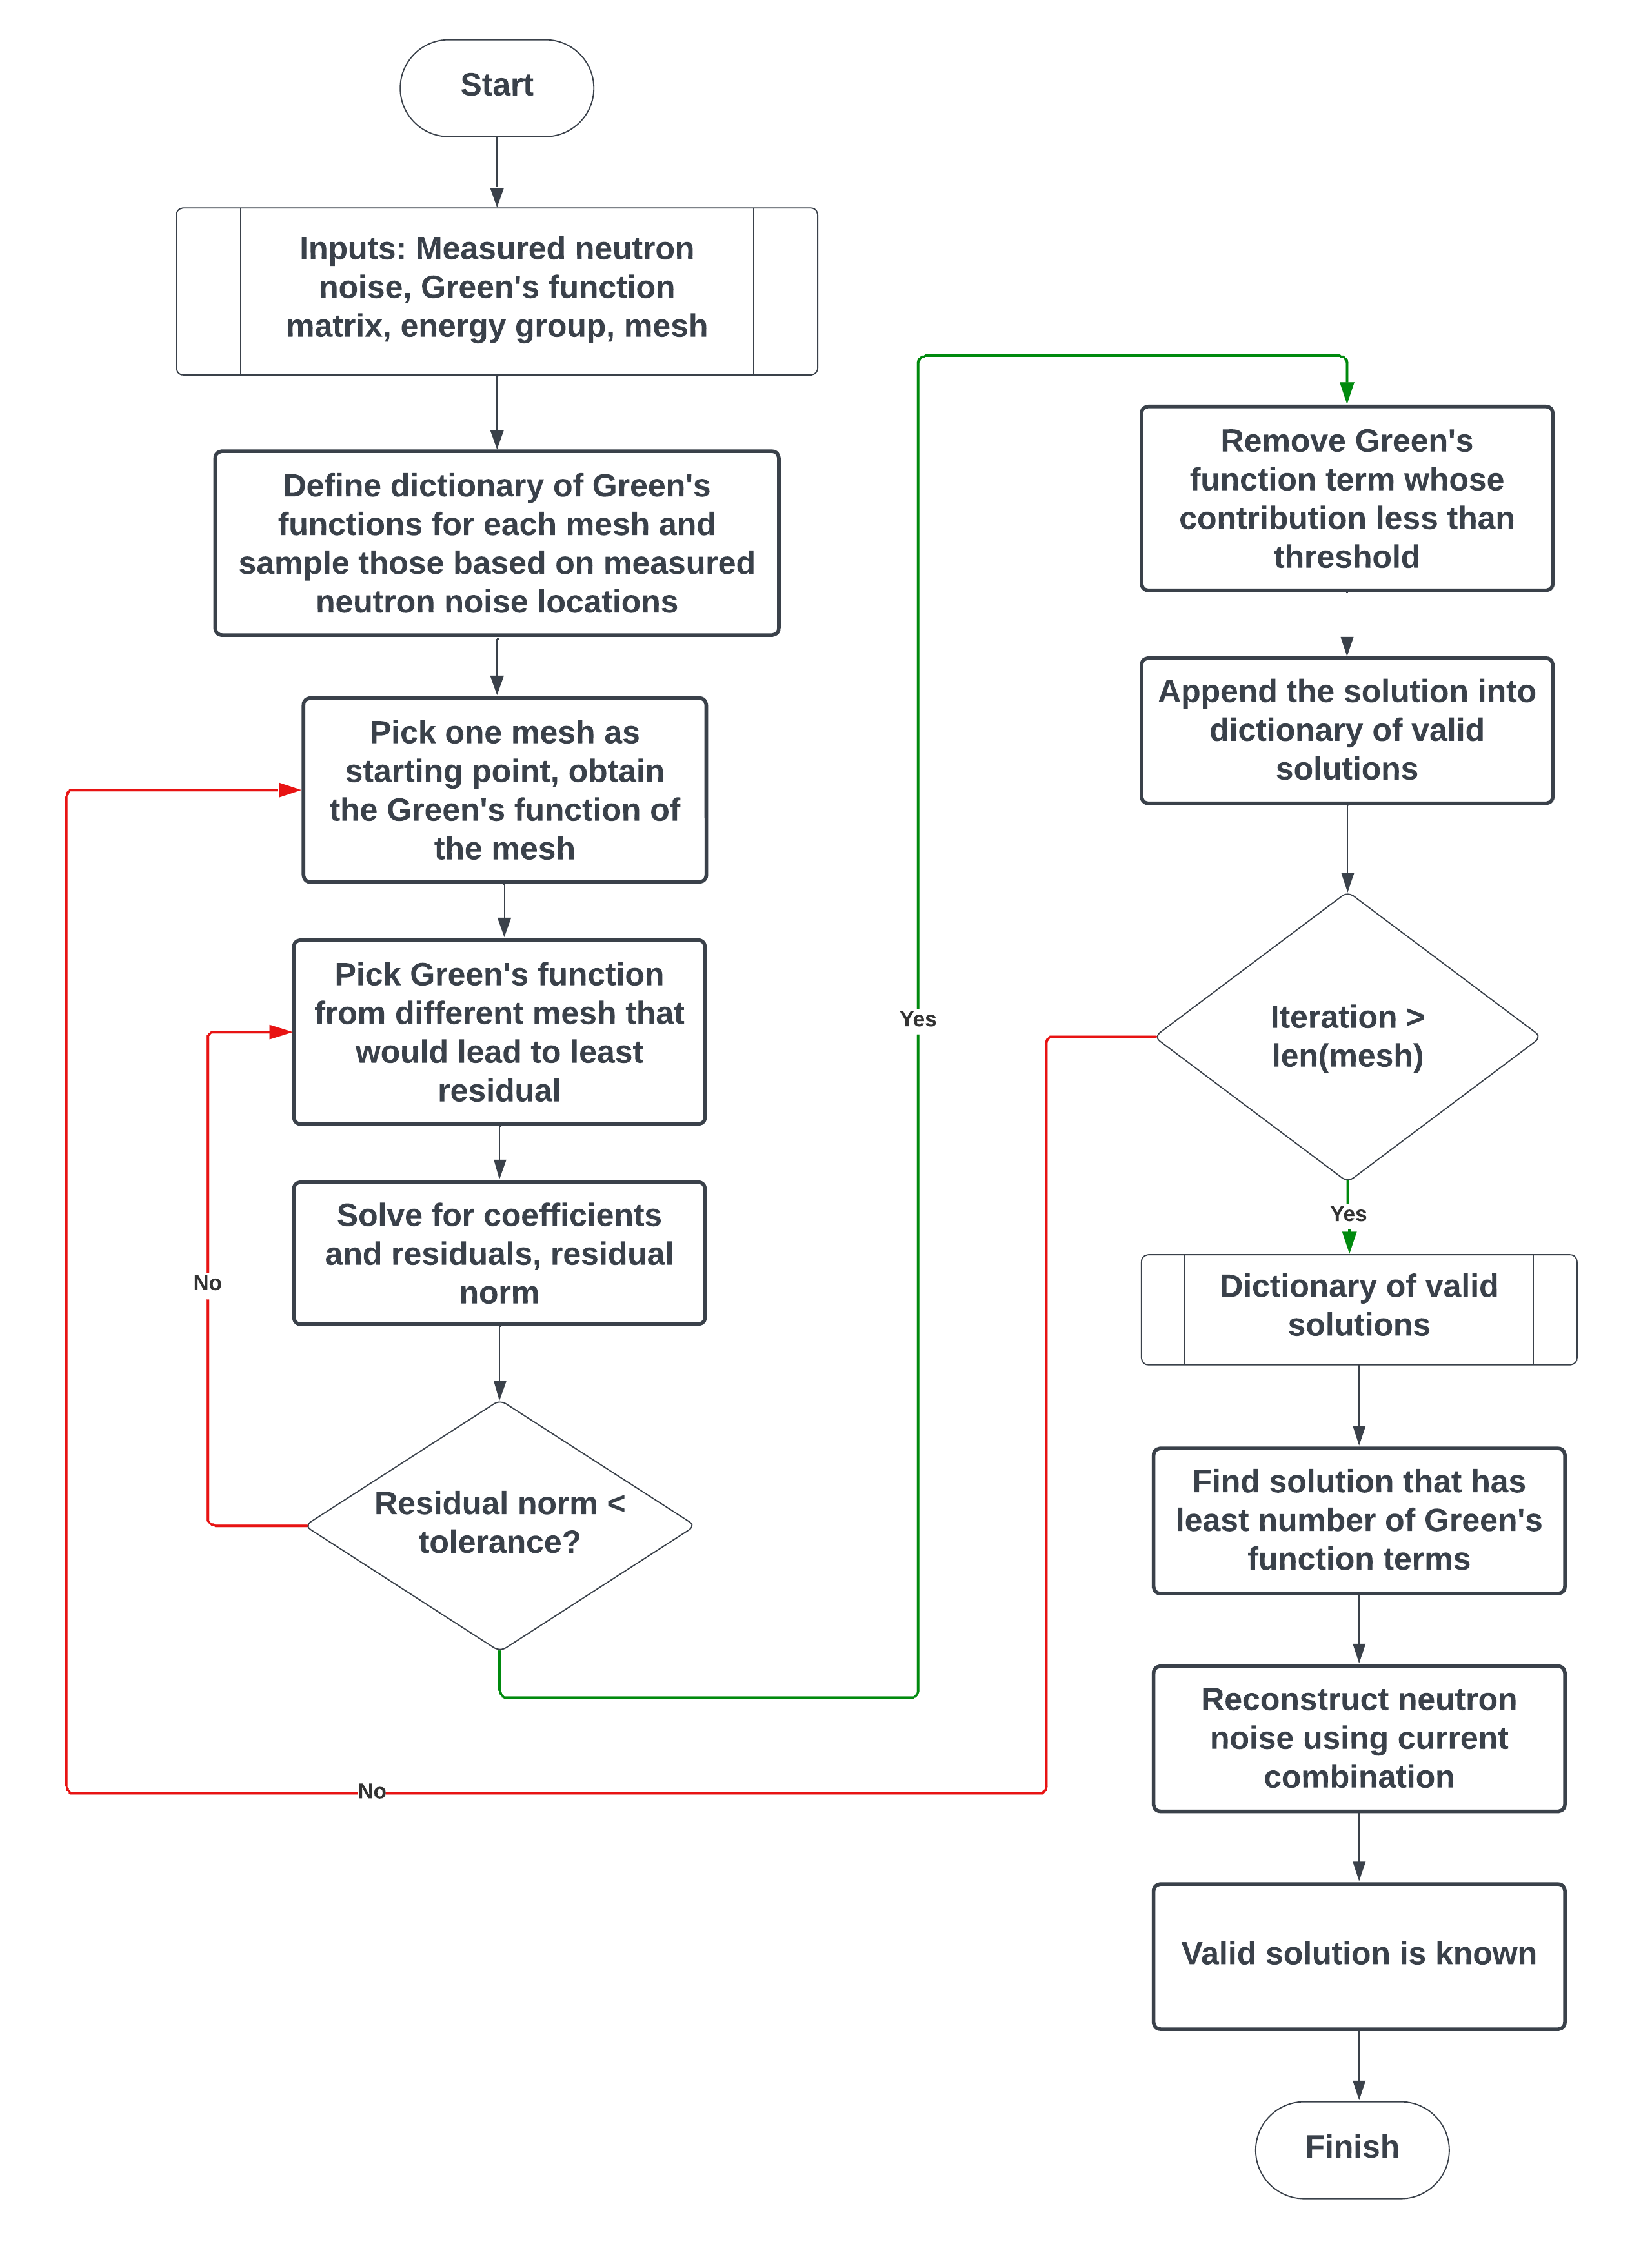
\includegraphics[width=0.6\textwidth]{figures/Greedy Method.png}
        \caption{Flow diagram of greedy method}
        \label{fig:greedy_method}
\end{figure}

The pseudo algorithm of the greedy method  is described in Algorithm~\ref{alg:greedy_unfold}.
\begin{algorithm}[H]
\caption{: Greedy Method}
\label{alg:greedy_unfold}
\begin{algorithmic}[1]
\Require Measured neutron noise $\delta \phi(\textbf{r}_{\text{meas}}, \omega)$, Green’s function matrix $G(\textbf{r}, \textbf{r}_p,\omega)$, energy groups $g$, mesh $N$
\Ensure reconstructed neutron noise $\delta \phi_{\text{GREEDY}}(\textbf{r}, \omega)$, unfolded source $S_{\text{GREEDY}}(\textbf{r}, \omega)$
\For{each group $g$} \Comment{\textbf{Construct Green’s function dictionary}}
    \For{each node $n$}
        \State Store columns of $G(\textbf{r}, \textbf{r}_p,\omega)$ in a dictionary
    \EndFor
\EndFor
\State Sample columns only at measured (non-zero) indices
\State Initialize solution sets: valid solutions $\gets \{\}$
\For{each candidate column $i$ in the dictionary subset} \Comment{\textbf{Greedy column selection}}
    \State Initialize residual $r \gets \delta \phi(\textbf{r}_{\text{meas}}, \omega)$
    \State Initialize selected column set $j^* \gets \{i\}$
    \While{$||\text{residual}||_2 > \text{tol}$}
        \State For each column $j \neq j*$, temporarily appended to the current selection $j^*$
        \State Compute the residual norm of the least squares fit with $S \cup \{j\}$
        \State Select column $j^*$ that minimizes residual norm
        \State Update $S \gets S \cup \{j^*\}$
        \State Update residual
    \EndWhile
    \State Recompute least-squares coefficients $\mathbf{c}$ of selected atom set $j^*$
    \State Remove columns with negligible contributions ($|c_i|/\max |c| < \tau$)    
    \State Store selected set $j^* \rightarrow$ valid solutions
\EndFor
\If{valid solutions exist} \Comment{\textbf{Select best solution}}
    \State Choose solution with minimal column count
    \State Compute reconstructed neutron noise: $\delta \phi_{\text{GREEDY}}(\textbf{r}, \omega) = \sum c_i G_i$
\Else
    \State \Return failure
\EndIf
\State Solve $S_{\text{GREEDY}}(\textbf{r}, \omega) = G^{-1}(\textbf{r}, \textbf{r}_p,\omega) \delta \phi_\text{GREEDY}(\textbf{r}, \omega)$
\State \textbf{Postprocess:} $S_{\text{GREEDY}}(\textbf{r}, \omega)$ file, $\delta \phi_\text{GREEDY}(\textbf{r}, \omega)$ file, plots. 
\end{algorithmic}
\end{algorithm}

This method is applied to unfold neutron noise sources for 2D and 3D HTTR geometries, which will be presented in Section \ref{sec:unfolding_application}.

\section{Application of HTTR Core}
\label{sec:unfolding_application}

In these cases, it is assumed that the detectors installed in the reactor can accurately measure neutron noise in both the fast and thermal energy groups. Any intrinsic detector noise is considered to have been removed, so the measured noise represents only the reactor-induced neutron noise. For the 2D HTTR case, there are 21 detectors that can accurately measure neutron noise. For the 3D HTTR case, there are also 21 detectors. Each detector can accurately detect neutron noise for the whole fuel column.

\subsection{2D HTTR with Absorber of Variable Strength Source}

\subsubsection{Single Noise Source}

In this simulation, a single mesh AVS source is unfolded using both the existing and novel methods. The simulation is done with a constant frequency of 1 Hz.  Figure \ref{fig:map_S_2DHTTR_AVS1S} shows the location of the AVS source.
\begin{figure}[H]
        \centering
        \begin{subfigure}{.48\textwidth}
          \centering
          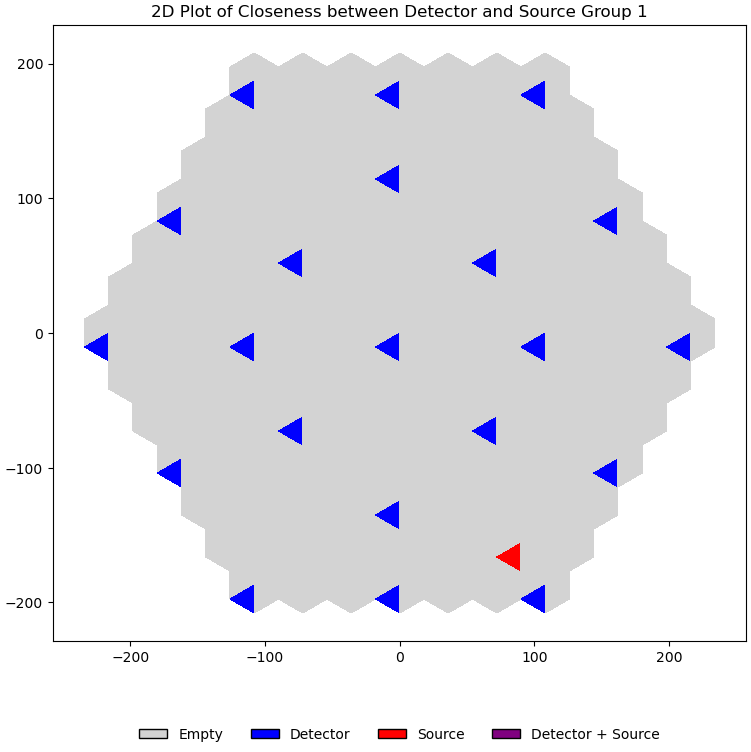
\includegraphics[width=\linewidth]{figures/OBJECTIVES6_TEST_SUITE_2DTriMG_HTTR_level1_iter2_closeness_det_S_categorical_G1.png}
        \end{subfigure}
        \hfill
        \begin{subfigure}{.48\textwidth}
          \centering
          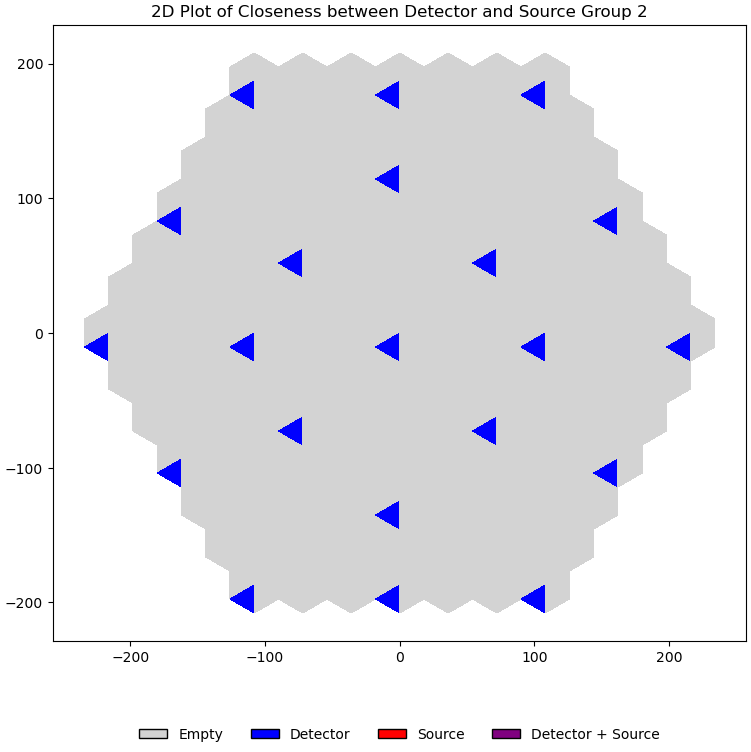
\includegraphics[width=\linewidth]{figures/OBJECTIVES6_TEST_SUITE_2DTriMG_HTTR_level1_iter2_closeness_det_S_categorical_G2.png}
        \end{subfigure}
        \caption{Location of source and detectors in the 2D HTTR case}
        \label{fig:map_S_2DHTTR_AVS1S}
\end{figure}

The results of the simulations are described in Table \ref{table:unfold_2DHTTR_AVS1S}.
\begin{table}[H]
        \centering
        \caption{Single noise source in 2D HTTR}
        \label{table:unfold_2DHTTR_AVS1S}
        \begin{tabular}{ | M{2cm} | M{1.5cm} | M{1.5cm} | M{4.5cm} | M{1.5cm} | } 
         \hline
         \textbf{Method} & \textbf{Energy Group} & \textbf{Hex Number} & \textbf{Neutron Noise Source} ($n/cm^3$) & \textbf{Match?}  \\
         \hline
         Reference & 1 & 14 & $-4.893 \times 10^{-5}+0.000i$ & --  \\
         \hline
         Inversion & 1 & 1 & $0.000+0.000i$ & No  \\
         \hline
         Zoning & 2 & 89 & $-5.635 \times 10^{-6}+4.056 \times 10^{-6}i$ & No  \\
         \hline
         Scanning & 1 & 14 & $-4.893 \times 10^{-5}+0.000i$ & Yes  \\
         \hline
         Brute Force & 1 & 14 & $-4.893 \times 10^{-5}+0.000i$ & Yes  \\
         \hline
         Greedy & 1 & 14 & $-4.893 \times 10^{-5}+0.000i$ & Yes  \\
         \hline
        \end{tabular}
\end{table}
The results show that the inversion and zoning method fails to unfold the neutron noise source. For the inversion method, this is due to the sparsity of the measured neutron noise, which results in poor interpolation quality. For the zoning method, it successfully identifies a location, but it is not the correct location of the neutron noise source. This is due to the limitation of the zoning method, where the number of fuel assemblies in each zone must be arranged in a specific way to match the number of detectors. On the other hand, scanning, brute force, and greedy methods manage to unfold the neutron noise source. This is an expected behavior. For the scanning method, it works well for a single mesh source, since it minimizes the difference between the neutron noise ratio and Green’s function ratio (See Eq. \ref{eq:scan_min}). The minimum difference is in the noise source location. For the brute force and greedy method, the method works well and matches the reference solution.

\subsubsection{Two Noise Sources}

In this simulation, a two-mesh AVS source is unfolded using both the existing and novel methods. The simulation is done with a constant frequency of 0.056 Hz. Figure \ref{fig:map_S_2DHTTR_AVS2S} shows the location of the AVS source.
\begin{figure}[H]
        \centering
        \begin{subfigure}{.48\textwidth}
          \centering
          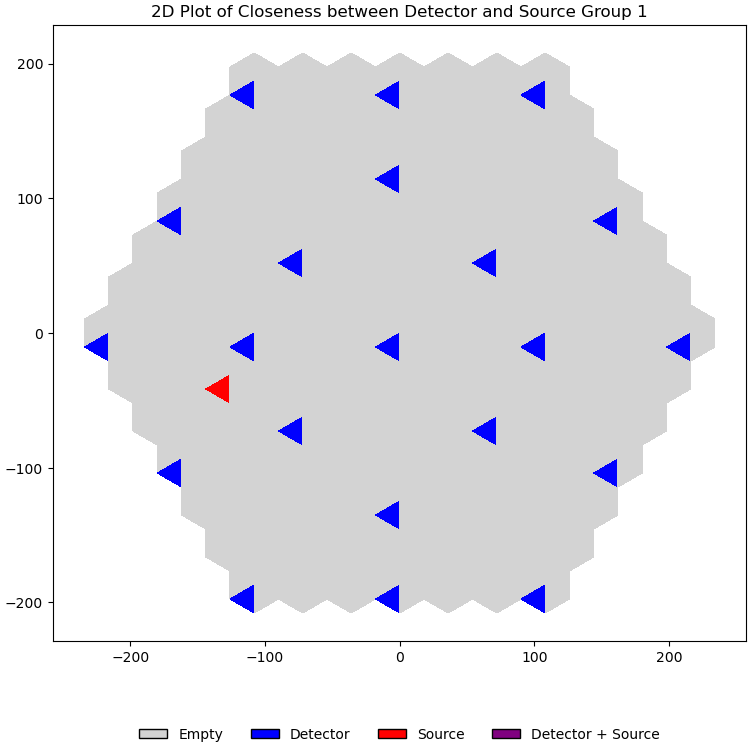
\includegraphics[width=\linewidth]{figures/OBJECTIVES6_TEST_SUITE_2DTriMG_HTTR_level1_iter18_closeness_det_S_categorical_G1.png}
        \end{subfigure}
        \hfill
        \begin{subfigure}{.48\textwidth}
          \centering
          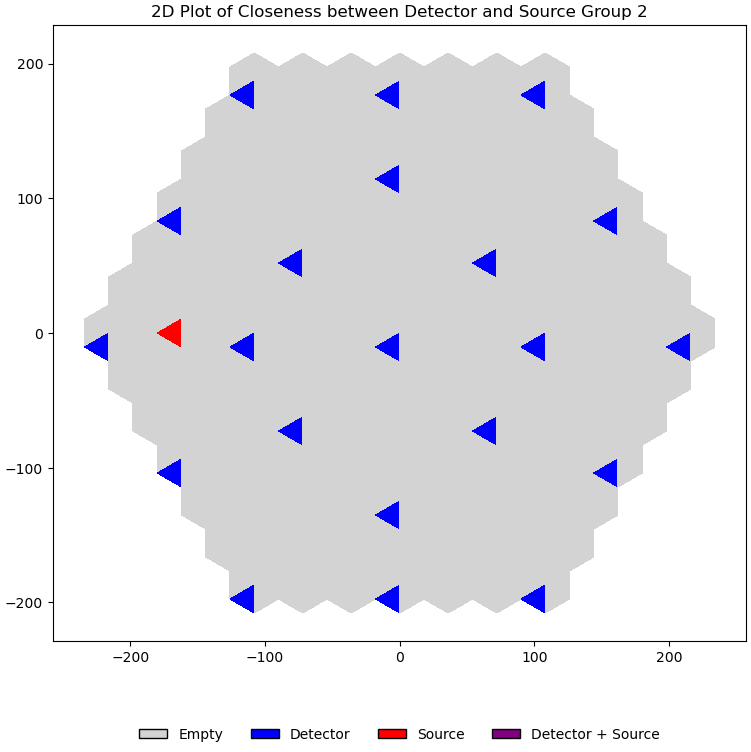
\includegraphics[width=\linewidth]{figures/OBJECTIVES6_TEST_SUITE_2DTriMG_HTTR_level1_iter18_closeness_det_S_categorical_G2.png}
        \end{subfigure}
        \caption{Location of sources and detectors in the 2D HTTR case}
        \label{fig:map_S_2DHTTR_AVS2S}
\end{figure}

The results of the simulations are described in Table \ref{table:unfold_2DHTTR_AVS2S}.
\begin{table}[H]
        \centering
        \caption{Two noise sources in 2D HTTR}
        \label{table:unfold_2DHTTR_AVS2S}
        \begin{tabular}{ | M{2cm} | M{1.5cm} | M{1.5cm} | M{4.5cm} | M{1.5cm} | } 
         \hline
         \textbf{Method} & \textbf{Energy Group} & \textbf{Hex Number} & \textbf{Neutron Noise Source} ($
         n/cm^3$) & \textbf{Match?}  \\
         \hline
         \multirow{2}{*}{Reference} & 1 & 48 & $-1.882 \times 10^{-3}+0.000i$ & --  \\
         \cline{2-5}                & 2 & 60 & $-5.189 \times 10^{-3}-4.670 \times 10^{-3}i$ & --  \\
         \hline
         \multirow{2}{*}{Inversion} & 1 & 1 & $0.000+0.000i$ & No  \\
         \cline{2-5}                & 1 & 2 & $0.000+0.000i$ & No  \\
         \hline
         \multirow{2}{*}{Zoning} & 1 & 86 & $-2.383 \times 10^{-3}+6.761 \times 10^{-4}i$ & No  \\
         \cline{2-5}             & 1 & 89 & $-2.201 \times 10^{-3}+9.212 \times 10^{-4}i$ & No  \\
         \hline
         \multirow{2}{*}{Scanning} & 2 & 60 & $-1.033 \times 10^{-2}-4.138 \times 10^{-3}i$ & No  \\
         \cline{2-5}               & 1 & 1 & $0.000+0.000i$ & No  \\
         \hline
         \multirow{2}{*}{Brute Force} & 1 & 48 & $-1.882 \times 10^{-3}+0.000i$ & Yes  \\
         \cline{2-5}                  & 2 & 60 & $-5.189 \times 10^{-3}-4.670 \times 10^{-3}i$ & Yes  \\
         \hline
         \multirow{2}{*}{Greedy} & 1 & 48 & $-1.882 \times 10^{-3}+0.000i$ & Yes  \\
         \cline{2-5}             & 2 & 60 & $-5.189 \times 10^{-3}-4.670 \times 10^{-3}i$ & Yes  \\
         \hline
        \end{tabular}
\end{table}
The results show that the inversion, zoning, and scanning method fails to unfold the neutron noise source. The inversion and zoning method is expected to fail, since it fails in a single source. The scanning method fails due to the method’s limitation, as it only points to one location that minimizes the ratio difference in Eq. \ref{eq:scan_min}. On the other hand, brute force and greedy methods manage to unfold the neutron noise source. This is expected behavior for both methods.

\subsubsection{Three Noise Sources}

In this simulation, a three-mesh AVS source is unfolded using both the existing and novel methods. The simulation is done with a constant frequency of 1 Hz. Figure \ref{fig:map_S_2DHTTR_AVS3S} shows the location of the AVS source.
\begin{figure}[H]
        \centering
        \begin{subfigure}{.48\textwidth}
          \centering
          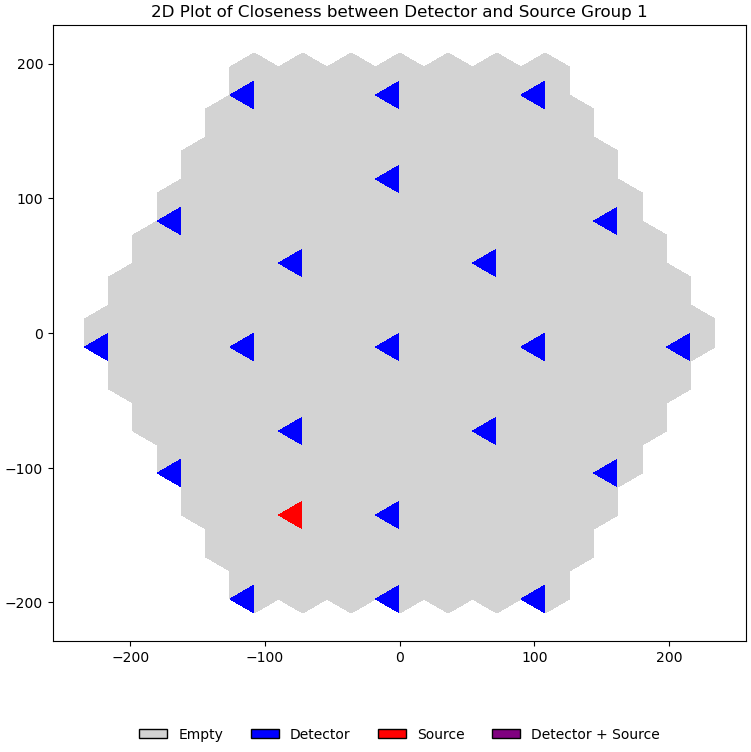
\includegraphics[width=\linewidth]{figures/OBJECTIVES45_TEST10_2DTriMG_HTTR_AVS3S_level1_closeness_det_S_categorical_G1.png}
        \end{subfigure}
        \hfill
        \begin{subfigure}{.48\textwidth}
          \centering
          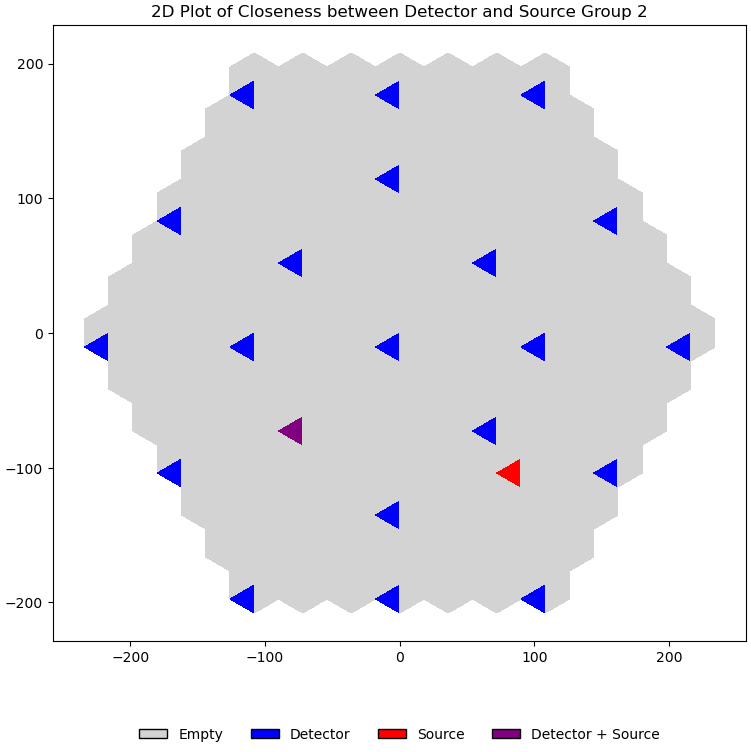
\includegraphics[width=\linewidth]{figures/OBJECTIVES45_TEST10_2DTriMG_HTTR_AVS3S_level1_closeness_det_S_categorical_G2.png}
        \end{subfigure}
        \caption{Location of sources and detectors in the 2D HTTR case}
        \label{fig:map_S_2DHTTR_AVS3S}
\end{figure}

The results of the simulations are described in Table \ref{table:unfold_2DHTTR_AVS3S}.
\begin{table}[H]
        \centering
        \caption{Three noise sources in 2D HTTR}
        \label{table:unfold_2DHTTR_AVS3S}
        \begin{tabular}{ | M{2cm} | M{1.5cm} | M{1.5cm} | M{4.5cm} | M{1.5cm} | } 
         \hline
         \textbf{Method} & \textbf{Energy Group} & \textbf{Hex Number} & \textbf{Neutron Noise Source} ($n/cm^3$) & \textbf{Match?}  \\
         \hline
         \multirow{3}{*}{Reference} & 1 & 18 & $-2.795 \times 10^{-8}+0.000i$ & --  \\
         \cline{2-5}                & 2 & 32 & $-3.342 \times 10^{-6}+0.000i$ & --  \\
         \cline{2-5}                & 2 & 38 & $-1.053 \times 10^{-4}+0.000i$ & --  \\
         \hline
         \multirow{3}{*}{Inversion} & 1 & 1 & $0.000+0.000i$ & No  \\
         \cline{2-5}                & 1 & 45 & $0.000+0.000i$ & No  \\
         \cline{2-5}                & 2 & 61 & $0.000+0.000i$ & No  \\
         \hline
         \multirow{3}{*}{Zoning} & 2 & 39 & $-1.915 \times 10^{-4}+9.311 \times 10^{-5}i$ & No \\
         \cline{2-5}             & 2 & 39 & $-1.753 \times 10^{-4}+9.751 \times 10^{-5}i$ & No \\
         \cline{2-5}             & 2 & 39 & $-1.648 \times 10^{-4}+8.764 \times 10^{-5}i$ & No \\
         \hline
         \multirow{3}{*}{Scanning} & 2 & 37 & $-1.062 \times 10^{-4}+1.096 \times 10^{-7}i$ & No  \\
         \cline{2-5}               & 1 & 1 & $0.000+0.000i$ & No  \\
         \cline{2-5}               & 1 & 2 & $0.000+0.000i$ & No  \\
         \hline
         \multirow{3}{*}{Brute Force} & 1 & 18 & $-2.795 \times 10^{-8}+0.000i$ & Yes  \\
         \cline{2-5}                  & 2 & 32 & $-3.342 \times 10^{-6}+0.000i$ & Yes  \\
         \cline{2-5}                  & 2 & 38 & $-1.053 \times 10^{-4}+0.000i$ & Yes  \\
         \hline
         \multirow{3}{*}{Greedy} & 1 & 18 & $-2.795 \times 10^{-8}+0.000i$ & Yes  \\
         \cline{2-5}             & 2 & 32 & $-3.342 \times 10^{-6}+0.000i$ & Yes  \\
         \cline{2-5}             & 2 & 38 & $-1.053 \times 10^{-4}+0.000i$ & Yes  \\
         \hline
        \end{tabular}
\end{table}
Similar to the two noise source problem, the results show that the inversion, zoning, and scanning method fails to unfold the neutron noise source. On the other hand, brute force and greedy methods manage to unfold the neutron noise source. This is expected behavior for both methods.

\subsection{3D HTTR with Absorber of Variable Strength Source}

\subsubsection{Single Noise Source}

In this simulation, a single mesh AVS source is unfolded using both the existing and novel methods. The simulation is done with a constant frequency of 1 Hz. The noise source is located at $Z=5$, thermal energy group. Figure \ref{fig:map_S_3DHTTR_AVS1S} shows the location of the AVS source.
\begin{figure}[H]
        \centering
        \begin{subfigure}{.48\textwidth}
          \centering
          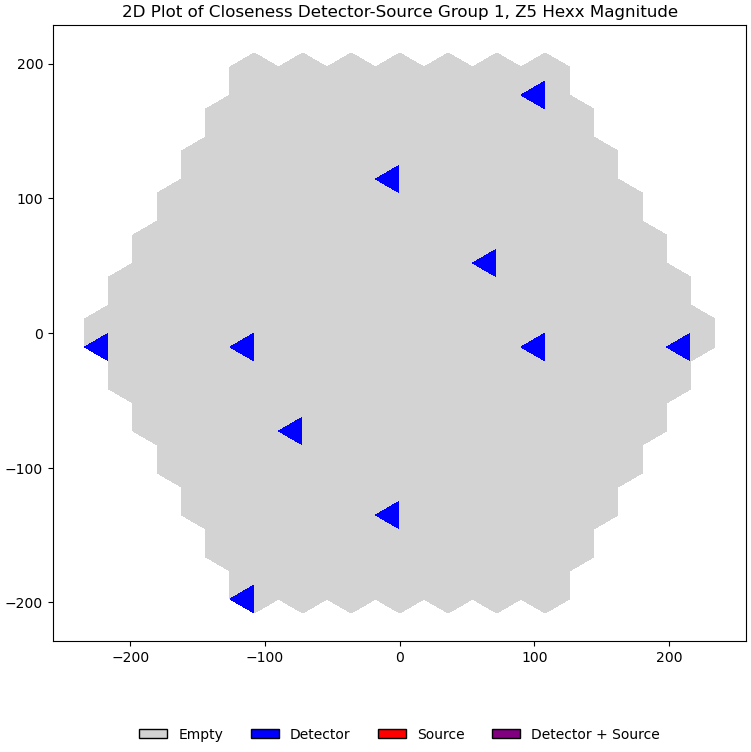
\includegraphics[width=\linewidth]{figures/OBJECTIVES45_TEST07_3DTriMG_HTTR_AVS_level1_closeness_det_S_categorical_G1_Z5.png}
        \end{subfigure}
        \hfill
        \begin{subfigure}{.48\textwidth}
          \centering
          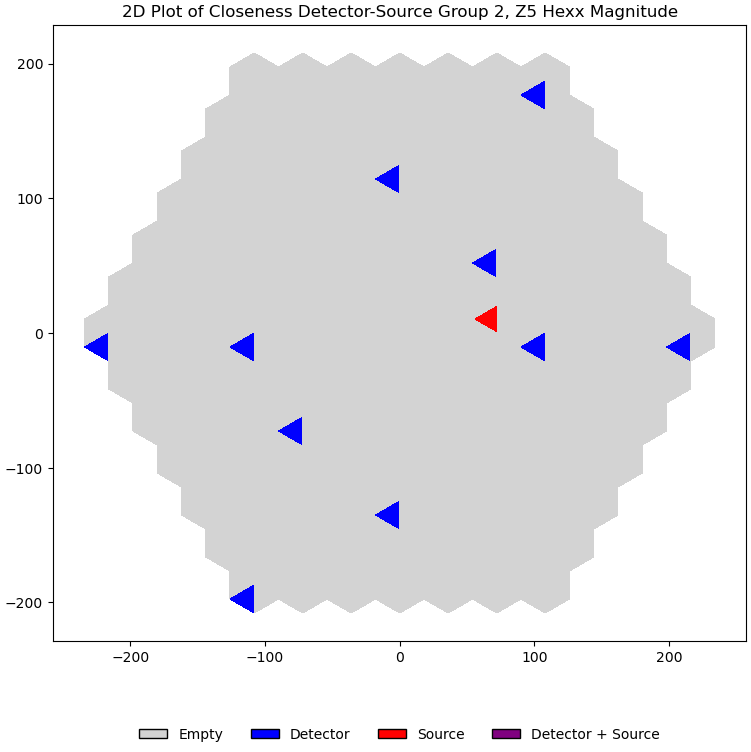
\includegraphics[width=\linewidth]{figures/OBJECTIVES45_TEST07_3DTriMG_HTTR_AVS_level1_closeness_det_S_categorical_G2_Z5.png}
        \end{subfigure}
        \caption{Location of source and detectors in the 3D HTTR single source case}
        \label{fig:map_S_3DHTTR_AVS1S}
\end{figure}

The results of the simulations are described in Table \ref{table:unfold_3DHTTR_AVS1S}.
\begin{table}[H]
        \centering
        \caption{Single noise source in 3D HTTR}
        \label{table:unfold_3DHTTR_AVS1S}
        \begin{tabular}{ | M{2cm} | M{1.5cm} | M{1.5cm} | M{1.5cm} | M{4cm} | M{1.5cm} | } 
         \hline
         \textbf{Method} & \textbf{Energy Group} & \textbf{Axial Level} & \textbf{Hex Number} & \textbf{Neutron Noise Source} ($n/cm^3$) & \textbf{Match?}  \\
         \hline
         Reference & 1 & 5 & 1 & $-4.912 \times 10^{-6} + 0.000i$ & -- \\
         \hline
         Inversion & 1 & 1 & 1 & $0.000 + 0.000i$ & No \\
         \hline
         Zoning & 2 & 3 & 9 & $-2.857 \times 10^{-6} + 0.000i$ & No \\
         \hline
         Scanning & 1 & 5 & 1 & $-4.912 \times 10^{-6} + 0.000i$ & Yes \\
         \hline
         Brute Force & 1 & 5 & 1 & $-4.912 \times 10^{-6} + 0.000i$ & Yes \\
         \hline
         Greedy & 1 & 5 & 1 & $-4.912 \times 10^{-6} + 0.000i$ & Yes \\
         \hline
        \end{tabular}
\end{table}
Similar to the results of a single mesh in the 2D HTTR case, the results show that the inversion and zoning method fails to unfold the neutron noise source. The scanning, brute force, and greedy methods manage to unfold the neutron noise source correctly. This is  expected behavior for the methods.

\subsubsection{Two Noise Source}

In this simulation, a two-mesh AVS source is unfolded using both the existing and novel methods. The simulation is done with a constant frequency of 1 Hz. There are 21 detectors in this case. Each detector can accurately detect neutron noise for the whole fuel column. The noise source is located in two different groups and axial levels. One source is located at $Z=4$ (near midplane) and fast group, while the other source is located at $Z=9$ (bottom of the core) and thermal group. Figure \ref{fig:map_S_3DHTTR_AVS2S} shows the location of the AVS source.
\begin{figure}[H]
        \centering
        \begin{subfigure}{.48\textwidth}
          \centering
          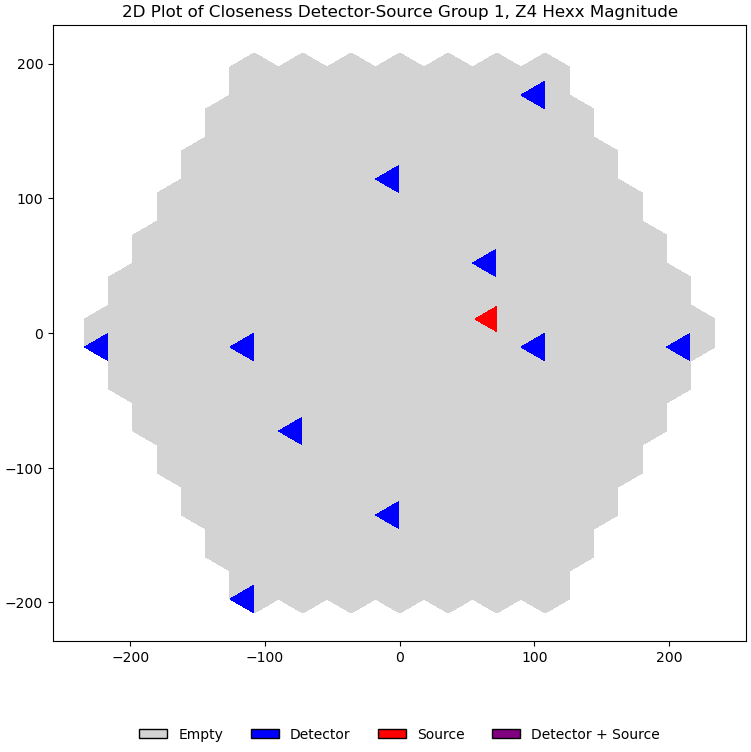
\includegraphics[width=\linewidth]{figures/OBJECTIVES45_TEST15_3DTriMG_HTTR_AVS2S_level1_closeness_det_S_categorical_G1_Z4.png}
        \end{subfigure}
        \hfill
        \begin{subfigure}{.48\textwidth}
          \centering
          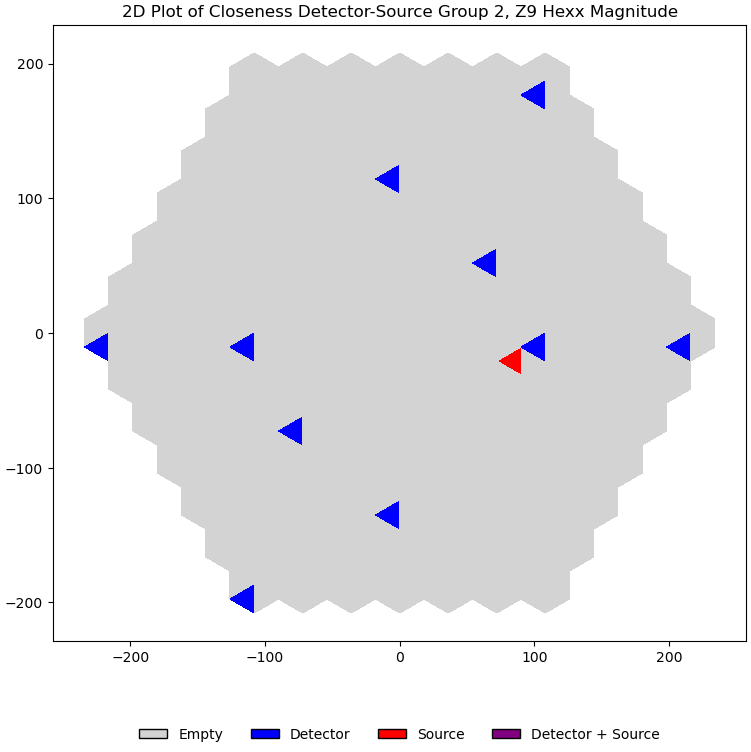
\includegraphics[width=\linewidth]{figures/OBJECTIVES45_TEST15_3DTriMG_HTTR_AVS2S_level1_closeness_det_S_categorical_G2_Z9.png}
        \end{subfigure}
        \caption{Location of source and detectors in the 3D HTTR two sources case}
        \label{fig:map_S_3DHTTR_AVS2S}
\end{figure}

The results of the simulations are described in Table \ref{table:unfold_3DHTTR_AVS2S}.
\begin{table}[H]
        \centering
        \caption{Two noise sources in 3D HTTR}
        \label{table:unfold_3DHTTR_AVS2S}
        \begin{tabular}{ | M{2cm} | M{1.5cm} | M{1.5cm} | M{1.5cm} | M{4.5cm} | M{1.5cm} | } 
         \hline
         \textbf{Method} & \textbf{Energy Group} & \textbf{Axial Level} & \textbf{Hex Number} & \textbf{Neutron Noise Source} ($n/cm^3$) & \textbf{Match?}  \\
         \hline
         \multirow{2}{*}{Reference} & 1 & 4 & 66 & $-2.922 \times 10^{-7} + 0.000i$ & -- \\
         \cline{2-6}                & 2 & 9 & 54 & $-3.152 \times 10^{-8} + 0.000i$ & -- \\
         \hline
         \multirow{2}{*}{Inversion} & 1 & 1 & 1 & $0.000 + 0.000i$ & No \\
         \cline{2-6}                & 1 & 1 & 2 & $0.000 + 0.000i$ & No \\
         \hline
         \multirow{2}{*}{Zoning} & 2 & 3 & 9 & $-1.395 \times 10^{-7} + 1.386 \times 10^{-7}i$ & No \\
         \cline{2-6}             & 2 & 3 & 3 & $-1.147 \times 10^{-7} + 1.105 \times 10^{-7}i$ & No \\
         \hline
         \multirow{2}{*}{Scanning} & 2 & 2 & 66 & $-2.423 \times 10^{-7} - 1.078 \times 10^{-9}i$ & No \\
         \cline{2-6}               & 1 & 4 & 1 & $0.000 + 0.000i$ & No \\
         \hline
         \multirow{2}{*}{Brute Force} & 1 & 4 & 66 & $-2.922 \times 10^{-7} + 0.000i$ & Yes \\
         \cline{2-6}                  & 2 & 9 & 54 & $-3.152 \times 10^{-8} + 0.000i$ & Yes \\
         \hline
         \multirow{2}{*}{Greedy} & 1 & 4 & 66 & $-2.922 \times 10^{-7} + 0.000i$ & Yes \\
         \cline{2-6}             & 2 & 9 & 54 & $-3.152 \times 10^{-8} + 0.000i$ & Yes \\
         \hline
        \end{tabular}
\end{table}
Similar to the two-mesh source of the 2D HTTR case, the results show that the inversion, zoning, and scanning method fail to unfold the neutron noise source. The inversion and zoning method is expected to fail, since it fails in a single source. The scanning method fails due to the method’s limitation, as it only points to one location that minimizes the ratio difference (see Eq. \ref{eq:scan_min}). On the other hand, brute force and greedy methods manage to unfold the neutron noise source. This is expected behavior for both methods.

\subsubsection{Three Mesh Source}

In this simulation, a three-mesh AVS source is unfolded using both the existing and novel methods. The simulation is done with a constant frequency of 1 Hz. There are 21 detectors in this case. Each detector can accurately detect neutron noise for the whole fuel column. The noise source is located in two different groups and axial levels. The first source is located at $Z=1$ (top of the core) and fast group, the second source is located at $Z=5$ (midplane) in thermal group, and the third source is located at $Z=9$ (bottom of the core) in thermal group. Figure \ref{fig:map_S_3DHTTR_AVS3S} shows the location of the AVS source.
\begin{figure}[H]
        \centering
        \begin{subfigure}{.48\textwidth}
          \centering
          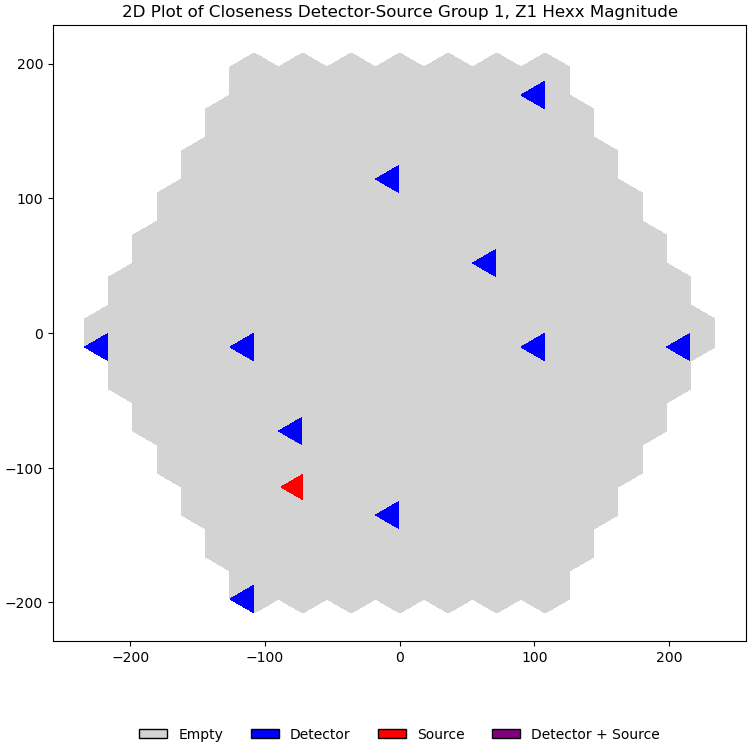
\includegraphics[width=\linewidth]{figures/OBJECTIVES45_TEST12_3DTriMG_HTTR_AVS3S_level1_closeness_det_S_categorical_G1_Z1.png}
        \end{subfigure}
        \hfill
        \begin{subfigure}{.48\textwidth}
          \centering
          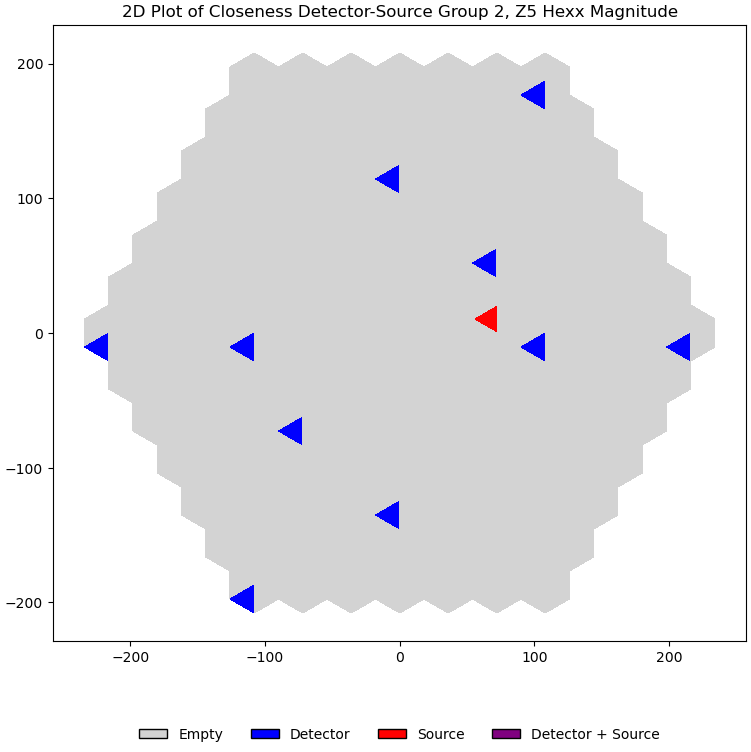
\includegraphics[width=\linewidth]{figures/OBJECTIVES45_TEST12_3DTriMG_HTTR_AVS3S_level1_closeness_det_S_categorical_G2_Z5.png}
        \end{subfigure}
        \hfill
        \begin{subfigure}{.48\textwidth}
          \centering
          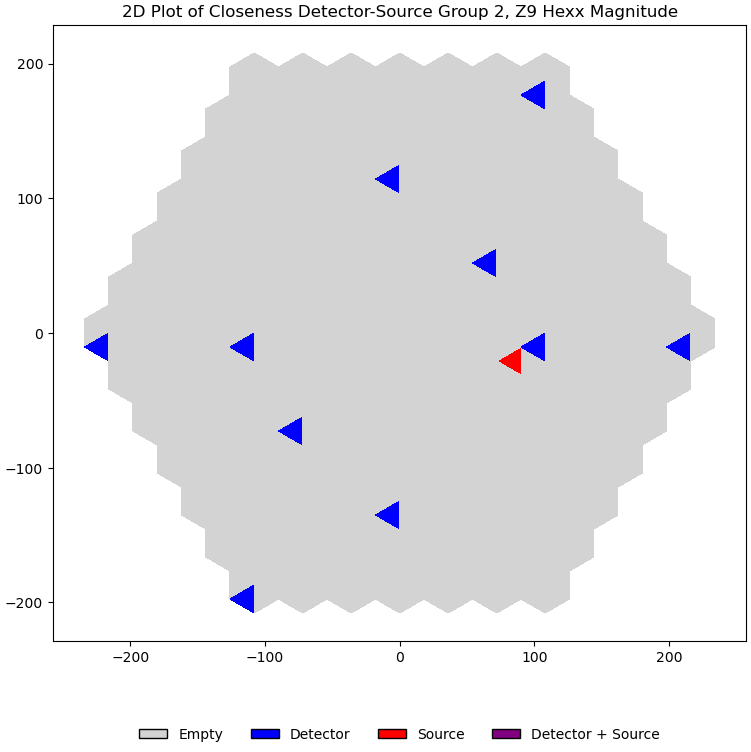
\includegraphics[width=\linewidth]{figures/OBJECTIVES45_TEST12_3DTriMG_HTTR_AVS3S_level1_closeness_det_S_categorical_G2_Z9.png}
        \end{subfigure}
        \caption{Location of source and detectors in the 3D HTTR three sources case}
        \label{fig:map_S_3DHTTR_AVS3S}
\end{figure}

The results of the simulations are described in Table \ref{table:unfold_3DHTTR_AVS3S}.
\begin{table}[H]
        \centering
        \caption{Three noise source in 3D HTTR}
        \label{table:unfold_3DHTTR_AVS3S}
        \begin{tabular}{ | M{2cm} | M{1.5cm} | M{1.5cm} | M{1.5cm} | M{4.5cm} | M{1.5cm} | } 
         \hline
         \textbf{Method} & \textbf{Energy Group} & \textbf{Axial Level} & \textbf{Hex Number} & \textbf{Neutron Noise Source} ($n/cm^3$) & \textbf{Match?}  \\
         \hline
         \multirow{2}{*}{Reference} & 1 & 1 & 18 & $-3.696 \times 10^{-10} + 0.000i$ & -- \\
         \cline{2-6}                & 2 & 5 & 66 & $-4.912 \times 10^{-6} + 0.000i$ & -- \\
         \cline{2-6}                & 2 & 9 & 54 & $-3.152 \times 10^{-8} + 0.000i$ & -- \\
         \hline
         \multirow{2}{*}{Inversion} & 1 & 1 & 1 & $0.000 + 0.000i$ & No \\
         \cline{2-6}                & 2 & 1 & 1 & $0.000 + 0.000i$ & No \\
         \cline{2-6}                & 2 & 1 & 2 & $0.000 + 0.000i$ & No \\
         \hline
         \multirow{2}{*}{Zoning} & 2 & 3 & 9 & $-3.339 \times 10^{-6} + 2.604 \times 10^{-6}i$ & No \\
         \cline{2-6}             & 2 & 3 & 3 & $-4.912 \times 10^{-6} + 2.078 \times 10^{-6}i$ & No \\
         \cline{2-6}             & 2 & 2 & 90 & $-3.152 \times 10^{-6} + 1.829 \times 10^{-6}i$  & No \\
         \hline
         \multirow{2}{*}{Scanning} & 2 & 2 & 66 & $-4.922 \times 10^{-6} - 1.243 \times 10^{-8}i$ & No \\
         \cline{2-6}               & 1 & 4 & 1 & $0.000 + 0.000i$ & No \\
         \cline{2-6}               & 1 & 4 & 2 & $0.000 + 0.000i$ & No \\
         \hline
         \multirow{2}{*}{Brute Force} & 1 & 1 & 18 & $-3.696 \times 10^{-10} + 0.000i$ & Yes \\
         \cline{2-6}                  & 2 & 5 & 66 & $-4.912 \times 10^{-6} + 0.000i$ & Yes \\
         \cline{2-6}                  & 2 & 9 & 54 & $-3.152 \times 10^{-8} + 0.000i$ & Yes \\
         \hline
         \multirow{2}{*}{Greedy} & 1 & 1 & 18 & $-3.696 \times 10^{-10} + 0.000i$ & Yes \\
         \cline{2-6}             & 2 & 5 & 66 & $-4.912 \times 10^{-6} + 0.000i$ & Yes \\
         \cline{2-6}             & 2 & 9 & 54 & $-3.152 \times 10^{-8} + 0.000i$ & Yes \\
         \hline
        \end{tabular}
\end{table}
Similar to the three-mesh source of 2D HTTR results, the results show that the inversion, zoning, and scanning method fails to unfold the neutron noise source. On the other hand, brute force and greedy methods are able to unfold the neutron noise source. This is expected behavior for both methods.

\section{Limitation of Novel Methods}

\subsection{Limitation of Brute Force Method}

The main limitation of the brute force method is the time necessary to calculate all combinations of Green’s function. Since the brute force iterates the process serially, the cost of the calculation grows exponentially. For example, the discretization used for 2D problem is relatively coarse. It solves for 1524 unknowns (2 groups x 762 mesh). Table \ref{table:brute_comb_number} shows the number of combinations that need to be solved in the brute force method for 2D HTTR. 
\begin{table}[H]
        \centering
        \caption{Number of combinations to solve in brute force method}
        \label{table:brute_comb_number}
        \begin{tabular}{ | M{2cm} | M{3cm} | } 
         \hline
         \textbf{Number of Sources} & \textbf{Number of Combinations} \\
         \hline
         1 & 1524 \\
         2 & 1.16 $\times 10^{6}$ \\
         3 & 5.89 $\times 10^{8}$ \\
         4 & 2.24 $\times 10^{11}$ \\
         \hline
        \end{tabular}
\end{table}
This makes the use of the brute force method computationally extremely expensive when the number of sources exceeds two.

\subsection{Limitation of Greedy Method}
\label{sec:greedy_limit}

The greedy method performs two iterations. The first iteration involves searching for a list of valid solutions by identifying the Green’s function component that leads to a local minimum residual. The second iteration aims to find a solution for the list of valid solutions that minimizes the residual within a certain tolerance and has the least amount of Green’s function components. It should be noted that residual in this case is the residual between the Green’s function combination and the measured neutron noise.

The quality and availability of the measured neutron noise data limit the performance of the greedy method. With a limited amount of measured neutron noise data, it would be possible to have an unfolding solution that is only partially correct (identifies some, but not all noise courses). This is because with limited measured neutron noise data, the residual calculation becomes under-constrained, meaning the greedy method may require more combinations of Green’s functions to reach the desired residual. Table \ref{table:greedy_source} shows the matching results for the greedy method applied to 2D HTTR for an increasing number of noise sources. The 2D HTTR core used in this case has 21 detectors, which means there are only 21 measured neutron noise data points. In these simulations, for each number of sources, the unfolding is repeated up to 10 times with different combinations of frequencies, magnitudes, energies, and locations. The sample values for these simulations are provided in Appendix \ref{ch:appendixC}. A similar simulation is done with 30 detectors to show the effect of availability of measured neutron noise data.
\begin{table}[H]
        \centering
        \caption{Reliability of greedy method with varying number of sources}
        \label{table:greedy_source}
        \begin{tabular}{ | M{2cm} | M{2.5cm} | M{2.5cm} |  M{2.5cm} | } 
         \hline
         \multirow{2}{=}{\centering\textbf{Number of Sources}} & 
         \multicolumn{2}{c|}{\textbf{Match Percentage}} \\ 
         \cline{2-3}
         &\textbf{21 Detectors} & \textbf{30 Detectors} \\
         \hline
         1 & 100\% & 100\% \\
         2 & 100\% & 100\% \\
         3 & 100\% & 100\% \\
         4 & 100\% & 100\% \\
         5 & 100\% & 100\% \\
         6 & 100\% & 100\% \\
         7 & 50\%  & 100\% \\
         \hline
        \end{tabular}
\end{table}

Table \ref{table:greedy_source} shows that with 21 measured neutron noise data, the greedy method can be reliable up to six noise sources. At seven noise sources, the greedy method becomes unreliable. However, using 30 measured neutron noise data, the reliability of the greedy method for seven noise sources is improved.

\section{Conclusion}

This chapter reviews the existing neutron noise unfolding methods and introduces novel methods that utilize Green’s function. The novel methods are the brute force method and the greedy method. The development of new methods is necessary, considering the limitations of the existing methods. The brute force method iterates through all combinations of Green’s function until it finds the combination that minimizes the residual below a certain tolerance. The greedy method is inspired by the matching pursuit algorithm in compressed sensing. In every iteration, it looks for the Green’s function component that minimizes the residual. This results in several valid solutions that overfit the residual. In the second step, the greedy method seeks a combination of Green’s functions from the valid solutions with the least number of components. 

Both the existing methods and the novel methods are applied to unfold neutron noise sources in the 2D HTTR and 3D HTTR core. The noise sources are defined as AVS-type sources. The unfolding is done using multiple AVS-type sources. The results show that the inversion and zoning methods are not reliable for unfolding neutron noise in HTTR. The scanning method is able to unfold only single neutron noise source and is unreliable for unfolding two or more sources. The brute force and greedy methods are effective in unfolding the neutron noise in the 2D and 3D HTTR core for at least 3 noise sources.

\chapter{Conclusions}
\label{ch:conclusions}

In this dissertation, computational method of neutron noise is introduced as a framework to detect anomalies in the HTGR core. This dissertation has two primary goals. First, we would like to introduce and apply the computational method of neutron noise analysis to a prismatic-type HTGR core, utilizing existing noise models to determine if neutron noise analysis can be generally applied to detect anomalies in advanced reactors, primarily prismatic-type HTGRs. The second goal is to two new methods of neutron noise unfolding. These methods are developed such that it can unfold multiple noise sources simultaneously. This is achieved by utilizing the Green's function, which has been employed in existing neutron noise unfolding methods.

The following sections provide a summary of the main findings, discuss how the research objectives have been addressed, and highlight possible directions for future work.

\section{Summary of Findings}

A literature review of neutron noise analysis is provided in Chapter \ref{ch:literature_review}. In this chapter, the theory and application of neutron noise are highlighted. The goal of this chapter is to provide a summary of past neutron noise analysis, which motivates the development of computational methods for neutron noise analysis. This chapter presents the derivation of the neutron noise equation from the multigroup diffusion equation in the frequency domain, as well as the derivation of other parameters crucial for neutron noise analysis. This includes the derivation of the point-kinetic and spatial components of the neutron noise, as well as the zero-power reactor transfer function. This chapter also provides examples of solvers developed to solve the neutron noise equation, utilizing both Monte Carlo and deterministic methods.

In Chapter \ref{ch:simulations}, a numerical solver to solve the forward, adjoint, and neutron noise equations is developed. This solver is capable of generating the Green's function matrix that will be used for the neutron noise unfolding methods. This solver is developed to fill the gap in the literature, particularly in terms of generating Green's functions in triangular geometries. The solver relies on a multigroup diffusion equation for energy and angular treatment, as well as a box-scheme finite difference method for spatial discretization. Sparse array matrices are used in the solver, which is solved using the PETSc Library. It is available in \href{https://github.com/harunardi/FANGS-UNFOLD}{GitHub} for future references. The solver has been verified with various benchmarks for both rectangular and triangular geometries. The results show that the numerical solver agrees well with numerical benchmarks and analytical solutions. This is true for the forward, adjoint, and neutron noise solutions.

In Chapter \ref{ch:noise_HTTR}, the chapter is divided into two main parts. The first part involves determining the characteristics of neutron noise in the HTTR. This is done by performing a neutron noise simulation to obtain the point-kinetic and spatial components of the neutron noise in HTTR, as well as by calculating the zero-power reactor transfer function (ZPRTF). Compared to LWRs, the neutron noise in HTTR generally follows the expected behavior of ZPRTF. A shorter plateau is observed in the ZPRTF of the HTTR case compared to other types of reactors. This means that the HTTR is more sensitive to perturbations at certain frequencies compared to other reactors. Using these results, we demonstrate that neutron noise analysis can be effectively utilized in the HTTR for core diagnostics. The second part of Chapter \ref{ch:noise_HTTR} is the application of neutron noise models in the HTTR core. The results show that for the AVS-type source, the neutron noise is more localized in the thermal group and more dispersed in the fast group. It is also observed that the point-kinetic component of the neutron noise is more dominant than the spatial component of neutron noise. For the fuel assembly vibration source, the results indicate that neutron noise has a significant impact on the overall vibration. This is more apparent when the neighboring assembly of the vibrating has a different characteristic (e.g., the neighboring assembly of the fuel assembly is a reflector assembly). 

In Chapter \ref{ch:unfolding_methods}, we introduced novel neutron noise unfolding methods, namely the brute force method and the greedy method. These methods are applied to unfold multiple AVS-type sources in 2D and 3D HTTR cores. As comparison, we also performed neutron noise unfolding using the existing method, namely the inversion method, zoning method, and scanning method. The results show that the inversion and zoning methods are not reliable for unfolding neutron noise in HTTR. The scanning method can unfold one AVS-type source, but fails to unfold two or three sources. The brute force and greedy methods can unfold the neutron noise in the 2D and 3D HTTR core. This demonstrates the capability of the novel method to unfold multiple neutron noise sources simultaneously.

\section{Future Works}

We have demonstrated how the neutron noise analysis can be applied to detect anomalies in a prismatic-type HTGR core. In doing so, we have shown that the neutron noise analysis can be performed in the HTGR core. We also introduced two novel methods for unfolding neutron noise in this study. We viewed this study as a starting point for exploring various topics in neutron noise analysis, particularly in the context of advanced reactor applications. For future work, we divide it into three categories:
\begin{itemize}
    \item For the numerical solver, we would argue that the use of the multigroup neutron diffusion equation is an industry standard. However, for spatial discretization, the nodal method is preferable in an industry setting. Therefore, the solver can be refactored to utilize the nodal method (e.g., polynomial expansion method) for the spatial discretization.
    \item For the application of neutron noise in the HTGR core, several engineering issues can be modeled and simulated using neutron noise analysis. One of those issues is the effect of flow-induced vibrations on the neutron economy and reactivity fluctuations. We argue that understanding flow-induced vibration through neutron noise analysis would be beneficial for detecting anomalies caused by vibration and assessing its impact on reactor operation.
    \item For the neutron noise unfolding methods, we can expand the utilization of the novel methods by optimizing the algorithm to obtain the correct combination of Green's functions. On the other hand, we can explore other algorithms to optimize the search algorithm. Pathfinding algorithms, such as Dijkstra's and A*, can be a good starting point in this case.
\end{itemize}

%%%%%%%%%%%%%%%%%%%%%%%%%%%%%%%%%%%%%%%%%%%%%%%%%%%%%%%%%%%%%%%%%%%%%%%%%%%%%%%
% per Graduate College preference, place the \appendix and the appendices content before the
% bibliography (here) only if the appendices contain references.
\backmatter

\printbibliography[heading=bibintoc,title={References}]

% the below lines are only needed if bibliography precedes appendices
% uses https://tex.stackexchange.com/a/440212 to continue page numbering
\clearpage
\setcounter{counterforappendices}{\value{page}}
\mainmatter
\setcounter{page}{\value{counterforappendices}}

\appendix

\chapter{Additional Cases of Forward, Adjoint, and Neutron Noise Simulations}
\label{ch:appendixA}

This appendix compiles all the cases simulated in this study as part of a sanity check to ensure that the solver works properly. Some of these cases were verified using other solvers, while others are simulations without comparison.

\section{2D C3 Benchmark}

The C3 reactor benchmark is a case for heterogeneous system. It is based on the C3 benchmark on deterministic transport calculations \cite{cavarecOECDNEABenchmark1994} and it is perturbed by introducing a localized neutron noise source. The system configuration is given in Figure \ref{fig:C3_configuration}. It consists of two UO2 fuel assemblies (at North-West and South-East positions) and two MOX fuel assemblies (at North-East and South-West positions). The size of each fuel assembly is 21.42 cm x 21.42 cm. The dark blue squares in the illustration are guide tubes; the ones in the center of the fuel assemblies contain fission chambers. Reflective boundary conditions are imposed. The perturbation is a fluctuation of 5\% of the fast and thermal neutron capture cross-sections in the fuel cell (16,19) identified with a red square in Figure \ref{fig:C3_configuration}.
\begin{figure}[H]
        \centering
        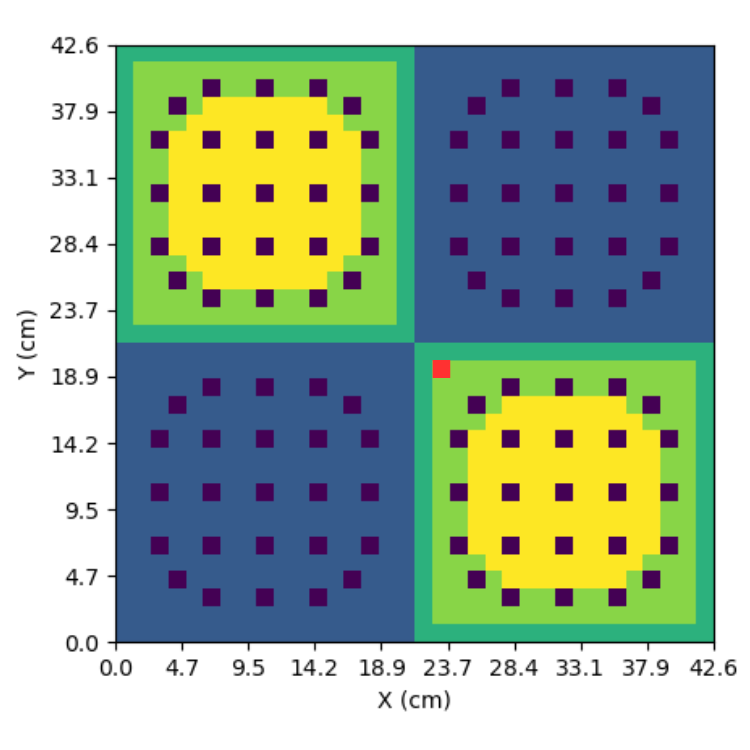
\includegraphics[width=0.6\textwidth]{figures/C3_configuration.png}
        \caption{Configuration of C3 Benchmark (obtained from \cite{mylonakisNeutronNoiseSimulations2019})}
        \label{fig:C3_configuration}
\end{figure}

For this simulation, CORE SIM+ results using finite difference are available. Therefore, the results from simulation will be compared to the CORE SIM+ results for forward flux, adjoint, and neutron noise calculation. The flux differences are calculated as relative error defined as follows:
\begin{equation}\label{eq:error1}
    \varepsilon = \frac{|\phi_{\text{solver}} - \phi_{\text{ref}}|}{|\phi_{\text{ref}}|} \times 100\%
\end{equation}

\subsection{Forward Flux Solution}

The forward flux solutions from CORE SIM+, the developed solver, and comparison between the simulators are as follow:
\begin{table}[H]
        \centering
        \caption{Eigenvalue comparison of 2D C3 Benchmark}
        \label{table:C3_fw_results}
        \begin{tabular}{ | M{3.5cm} | M{2cm} | } 
         \hline
         $k_{\text{eff}}$ CORE SIM+ & 1.019060  \\
         \hline
         $k_{\text{eff}}$ solver & 1.019060  \\
         \hline
         Absolute Error (pcm) & 0.0  \\
         \hline
        \end{tabular}
\end{table}

\begin{figure}[H]
        \centering
        \begin{subfigure}{.48\textwidth}
          \centering
          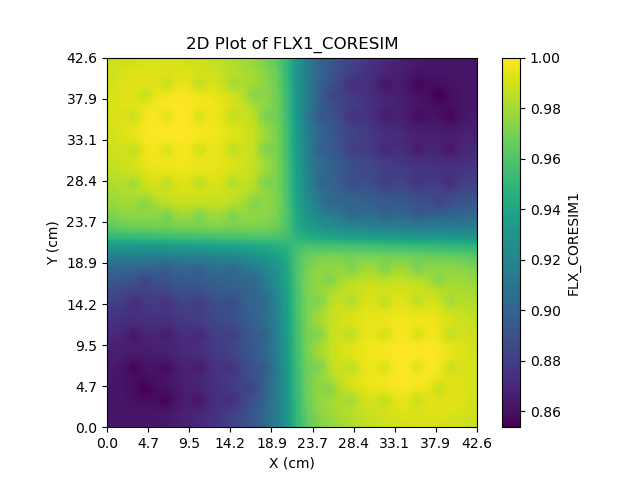
\includegraphics[width=\linewidth]{figures/OBJECTIVES1_TEST02_2DMG_C3_VandV_FORWARD_FLX_CORESIM_G1.png}
        \end{subfigure}
        \hfill
        \begin{subfigure}{.48\textwidth}
          \centering
          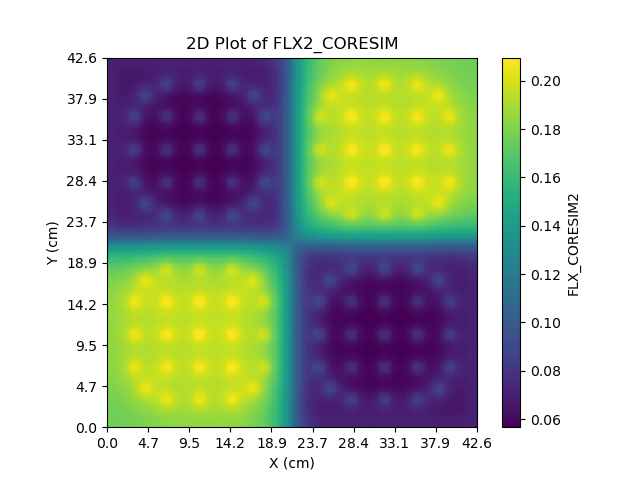
\includegraphics[width=\linewidth]{figures/OBJECTIVES1_TEST02_2DMG_C3_VandV_FORWARD_FLX_CORESIM_G2.png}
        \end{subfigure}
        \caption{Forward flux results from CORE SIM+}
        \label{fig:C3_fw_results_flx}
\end{figure}
\begin{figure}[H]
        \centering
        \begin{subfigure}{.48\textwidth}
          \centering
          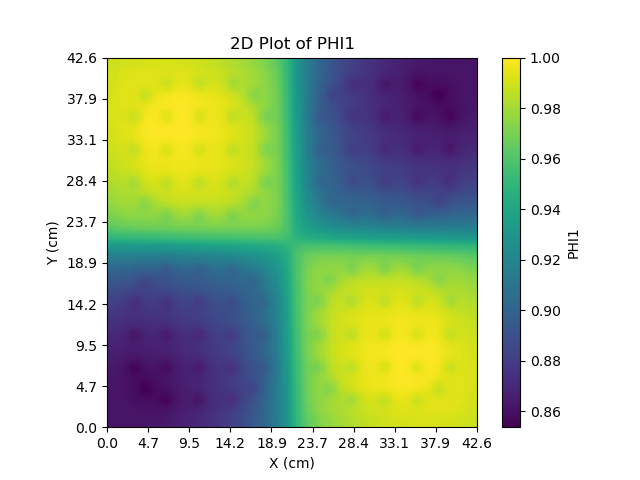
\includegraphics[width=\linewidth]{figures/OBJECTIVES1_TEST02_2DMG_C3_VandV_FORWARD_PHI_G1.png}
        \end{subfigure}
        \hfill
        \begin{subfigure}{.48\textwidth}
          \centering
          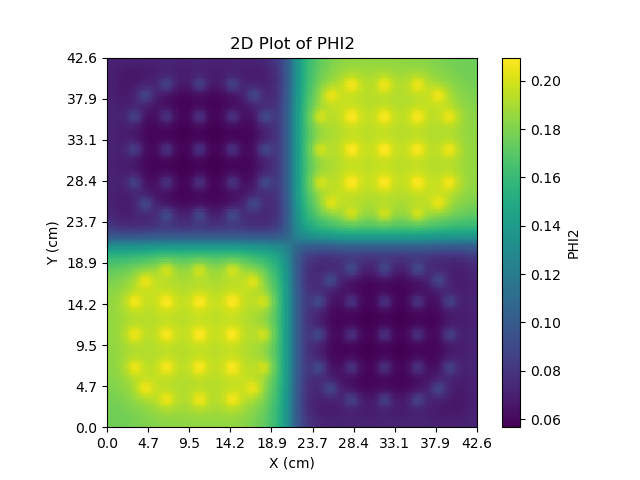
\includegraphics[width=\linewidth]{figures/OBJECTIVES1_TEST02_2DMG_C3_VandV_FORWARD_PHI_G2.png}
        \end{subfigure}
        \caption{Forward flux results from the developed solver}
        \label{fig:C3_fw_results_phi}
\end{figure}
\begin{figure}[H]
        \centering
        \begin{subfigure}{.48\textwidth}
          \centering
          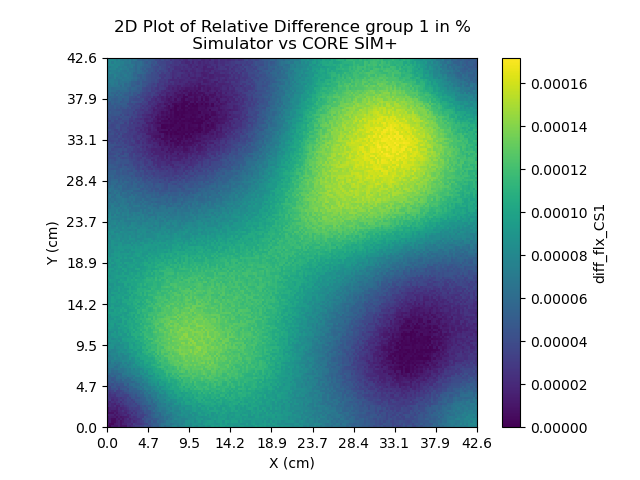
\includegraphics[width=\linewidth]{figures/OBJECTIVES1_TEST02_2DMG_C3_VandV_FORWARD_diff_flx_CS_G1.png}
        \end{subfigure}
        \hfill
        \begin{subfigure}{.48\textwidth}
          \centering
          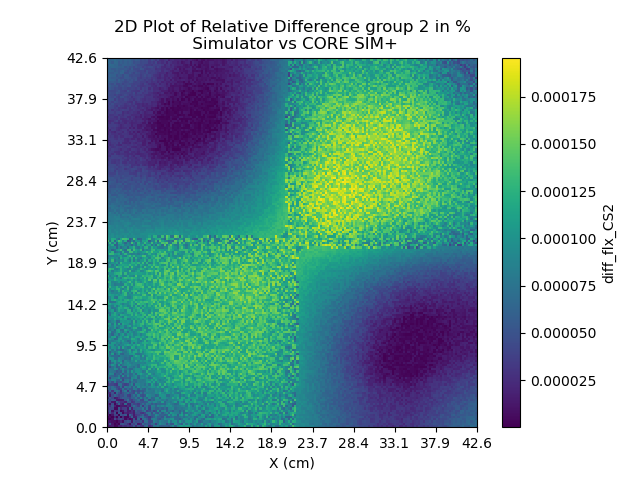
\includegraphics[width=\linewidth]{figures/OBJECTIVES1_TEST02_2DMG_C3_VandV_FORWARD_diff_flx_CS_G2.png}
        \end{subfigure}
        \caption{Difference of forward flux between CORE SIM+ and the solver}
        \label{fig:C3_fw_results_diff_phi}
\end{figure}

As seen in Table \ref{table:C3_fw_results}, Figure \ref{fig:C3_fw_results_flx}, Figure \ref{fig:C3_fw_results_phi}, and Figure \ref{fig:C3_fw_results_diff_phi}, the results show that the solver agrees well with CORE SIM+. The $k_{\text{eff}}$ matches between CORE SIM+ and solver exactly. This is due to the fact that this solver uses similar discretization to CORE SIM+. The error is less than 1\% for the forward flux. This shows that the solver works well for 2D rectangular geometries.

\subsection{Adjoint Flux Solution}

The adjoint flux solutions from CORE SIM+, the developed solver, and comparison between the simulators are as follows:
\begin{figure}[H]
        \centering
        \begin{subfigure}{.48\textwidth}
          \centering
          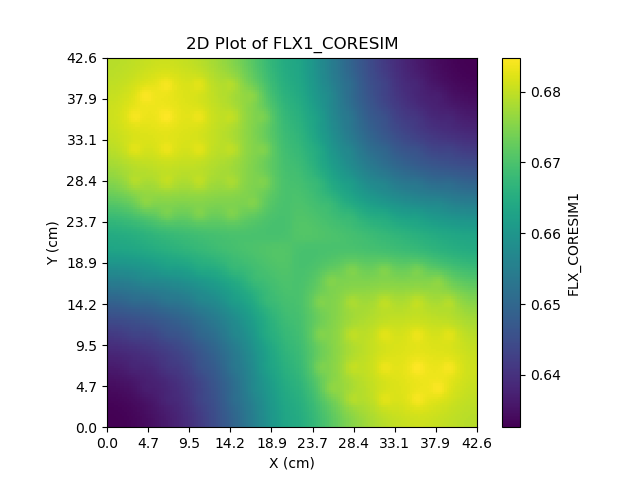
\includegraphics[width=\linewidth]{figures/OBJECTIVES1_TEST02_2DMG_C3_VandV_ADJOINT_FLX_CORESIM_G1.png}
        \end{subfigure}
        \hfill
        \begin{subfigure}{.48\textwidth}
          \centering
          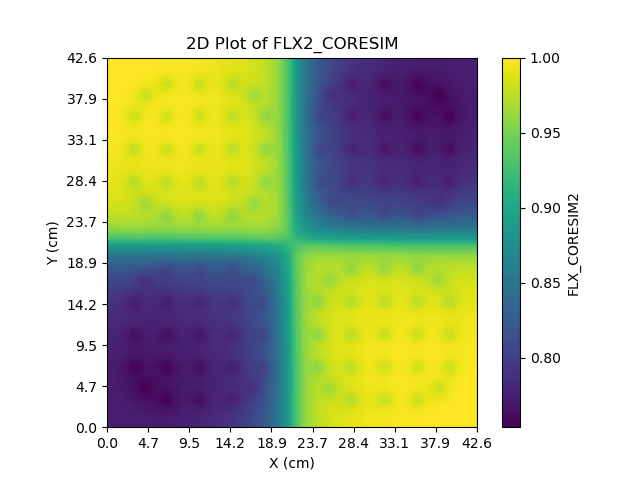
\includegraphics[width=\linewidth]{figures/OBJECTIVES1_TEST02_2DMG_C3_VandV_ADJOINT_FLX_CORESIM_G2.png}
        \end{subfigure}
        \caption{Adjoint flux results from CORE SIM+}
        \label{fig:C3_adj_results_flx}
\end{figure}
\begin{figure}[H]
        \centering
        \begin{subfigure}{.48\textwidth}
          \centering
          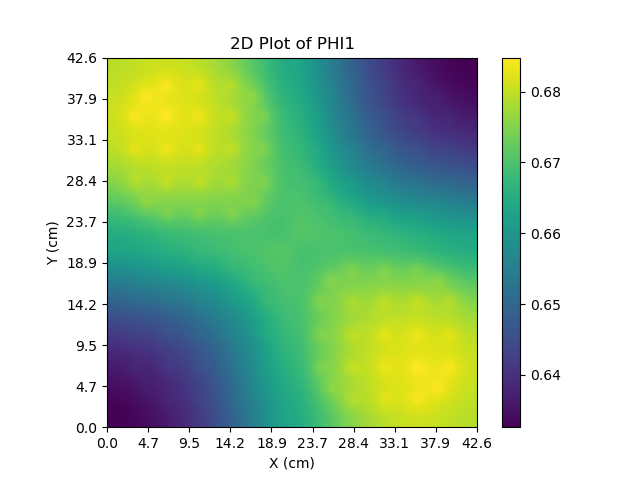
\includegraphics[width=\linewidth]{figures/OBJECTIVES1_TEST02_2DMG_C3_VandV_ADJOINT_PHI_G1.png}
        \end{subfigure}
        \hfill
        \begin{subfigure}{.48\textwidth}
          \centering
          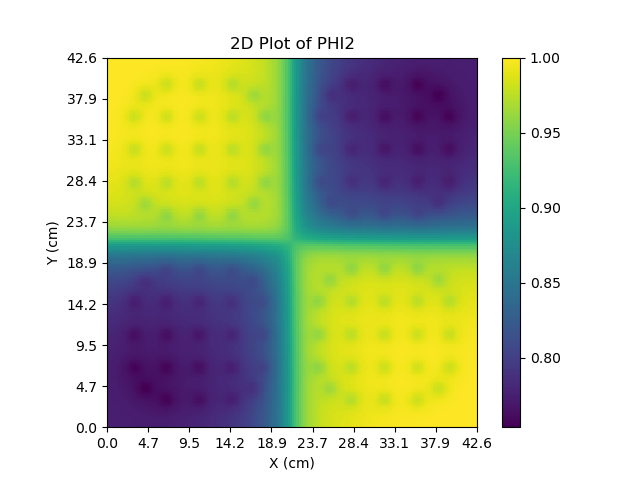
\includegraphics[width=\linewidth]{figures/OBJECTIVES1_TEST02_2DMG_C3_VandV_ADJOINT_PHI_G2.png}
        \end{subfigure}
        \caption{Adjoint flux results from the developed solver}
        \label{fig:C3_adj_results_phi}
\end{figure}
\begin{figure}[H]
        \centering
        \begin{subfigure}{.48\textwidth}
          \centering
          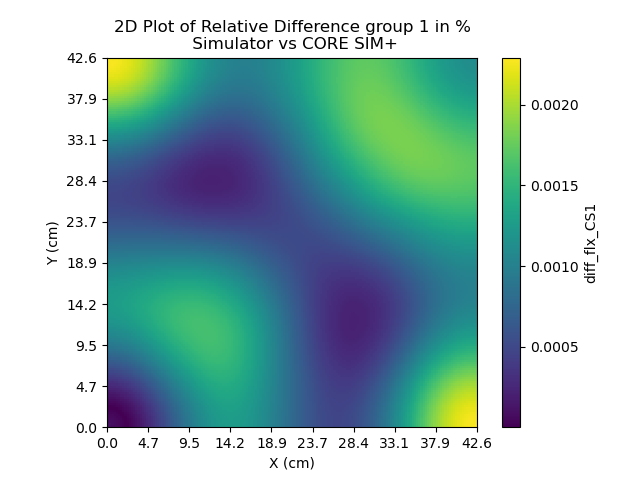
\includegraphics[width=\linewidth]{figures/OBJECTIVES1_TEST02_2DMG_C3_VandV_ADJOINT_diff_flx_CS_G1.png}
        \end{subfigure}
        \hfill
        \begin{subfigure}{.48\textwidth}
          \centering
          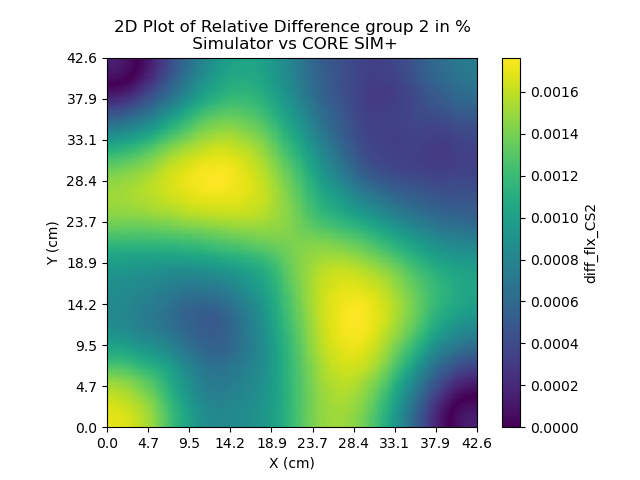
\includegraphics[width=\linewidth]{figures/OBJECTIVES1_TEST02_2DMG_C3_VandV_ADJOINT_diff_flx_CS_G2.png}
        \end{subfigure}
        \caption{Difference of adjoint flux between CORE SIM+ and the solver}
        \label{fig:C3_adj_results_diff_phi}
\end{figure}

As seen in Figure \ref{fig:C3_adj_results_flx}, Figure \ref{fig:C3_adj_results_phi}, and Figure \ref{fig:C3_adj_results_diff_phi}, the results show that the solver agrees well with CORE SIM+. Similar to the forward case, the error is less than 1\% for the adjoint flux. This shows that the solver works well for 2D rectangular geometries to calculate adjoint equation.

\subsection{Neutron Noise Solution}

The neutron noise solutions from CORE SIM+, the developed solver, and comparison between the simulators are shown in Figures \ref{fig:C3_noise_results_flx} - \ref{fig:C3_noise_results_diff_phi}.
\newpage
\begin{figure}[H]
        \centering
        \begin{subfigure}{.48\textwidth}
          \centering
          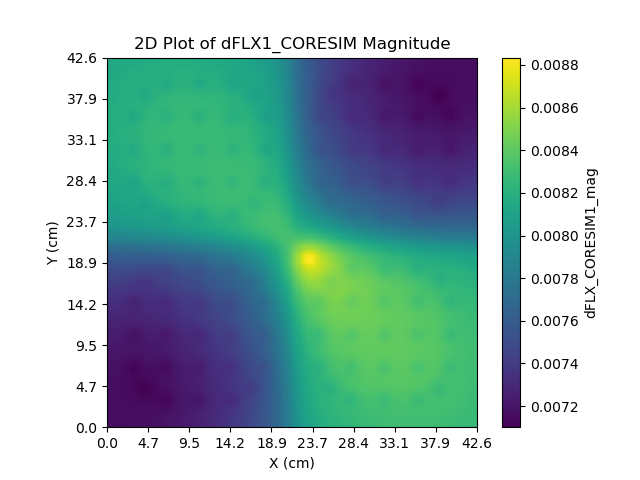
\includegraphics[width=\linewidth]{figures/OBJECTIVES1_TEST02_2DMG_C3_VandV_NOISE_dFLX_CORESIM_magnitude_G1.png}
        \end{subfigure}
        \hfill
        \begin{subfigure}{.48\textwidth}
          \centering
          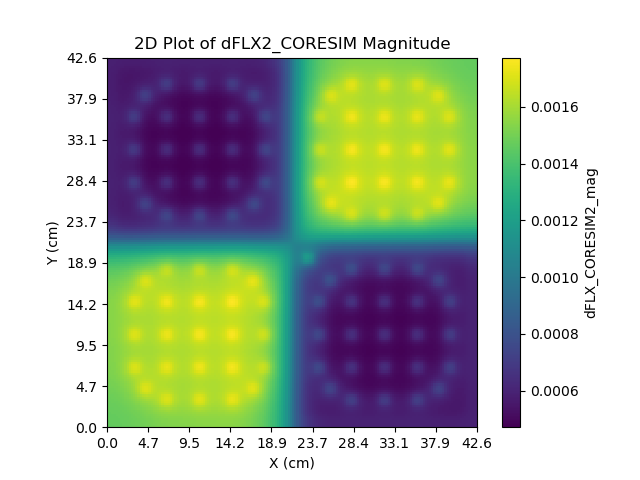
\includegraphics[width=\linewidth]{figures/OBJECTIVES1_TEST02_2DMG_C3_VandV_NOISE_dFLX_CORESIM_magnitude_G2.png}
        \end{subfigure}
\end{figure}
\begin{figure}[H]\ContinuedFloat
        \centering
        \begin{subfigure}{.48\textwidth}
          \centering
          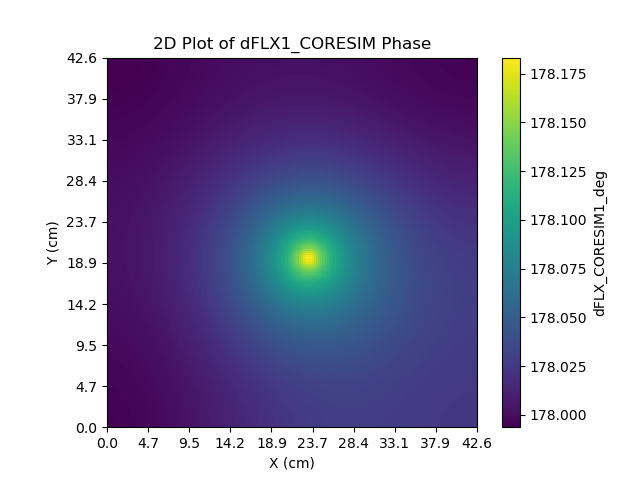
\includegraphics[width=\linewidth]{figures/OBJECTIVES1_TEST02_2DMG_C3_VandV_NOISE_dFLX_CORESIM_phase_G1.png}
        \end{subfigure}
        \hfill
        \begin{subfigure}{.48\textwidth}
          \centering
          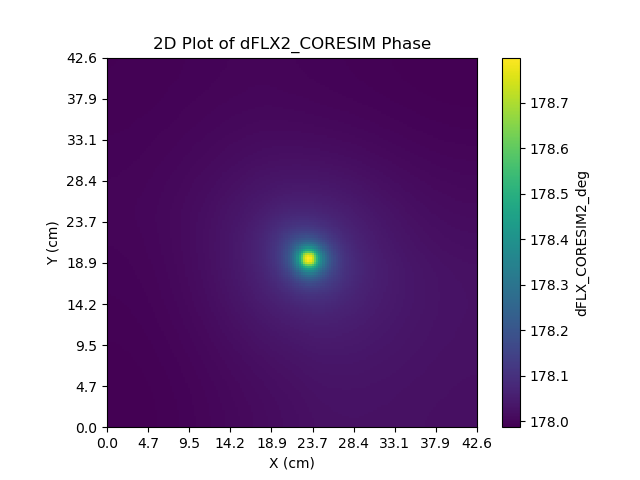
\includegraphics[width=\linewidth]{figures/OBJECTIVES1_TEST02_2DMG_C3_VandV_NOISE_dFLX_CORESIM_phase_G2.png}
        \end{subfigure}
        \caption{Neutron noise results from CORE SIM+}
        \label{fig:C3_noise_results_flx}
\end{figure}

\newpage
\begin{figure}[H]
        \centering
        \begin{subfigure}{.48\textwidth}
          \centering
          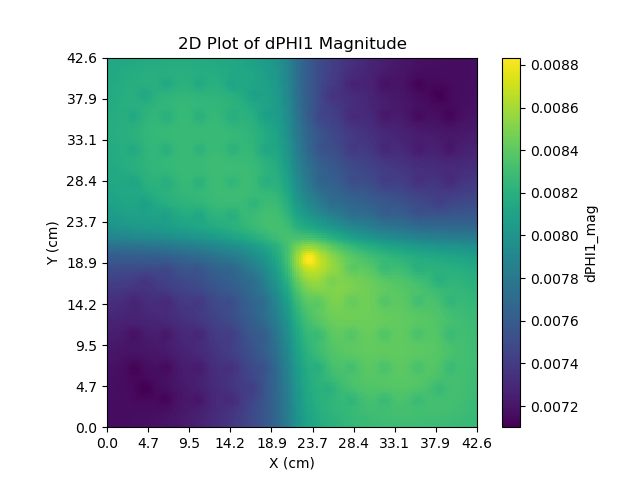
\includegraphics[width=\linewidth]{figures/OBJECTIVES1_TEST02_2DMG_C3_VandV_NOISE_dPHI_magnitude_G1.png}
        \end{subfigure}
        \hfill
        \begin{subfigure}{.48\textwidth}
          \centering
          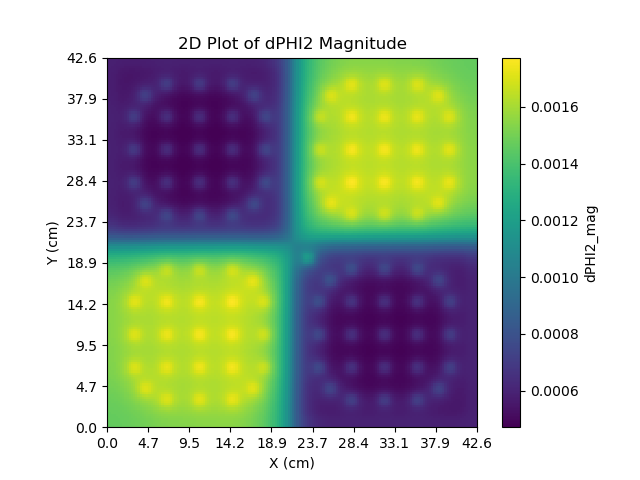
\includegraphics[width=\linewidth]{figures/OBJECTIVES1_TEST02_2DMG_C3_VandV_NOISE_dPHI_magnitude_G2.png}
        \end{subfigure}
\end{figure}
\begin{figure}[H]\ContinuedFloat
        \centering
        \begin{subfigure}{.48\textwidth}
          \centering
          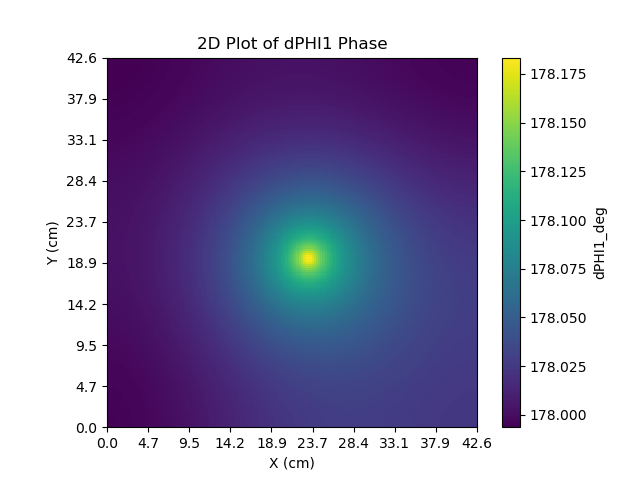
\includegraphics[width=\linewidth]{figures/OBJECTIVES1_TEST02_2DMG_C3_VandV_NOISE_dPHI_phase_G1.png}
        \end{subfigure}
        \hfill
        \begin{subfigure}{.48\textwidth}
          \centering
          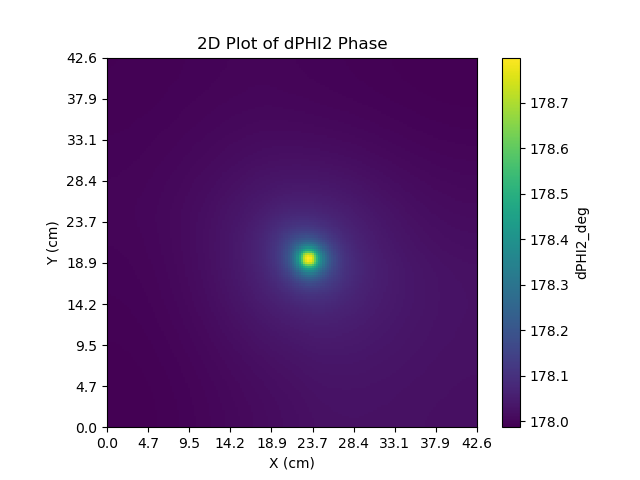
\includegraphics[width=\linewidth]{figures/OBJECTIVES1_TEST02_2DMG_C3_VandV_NOISE_dPHI_phase_G2.png}
        \end{subfigure}
        \caption{Neutron noise results from the developed solver}
        \label{fig:C3_noise_results_phi}
\end{figure}

\newpage
\begin{figure}[H]
        \centering
        \begin{subfigure}{.48\textwidth}
          \centering
          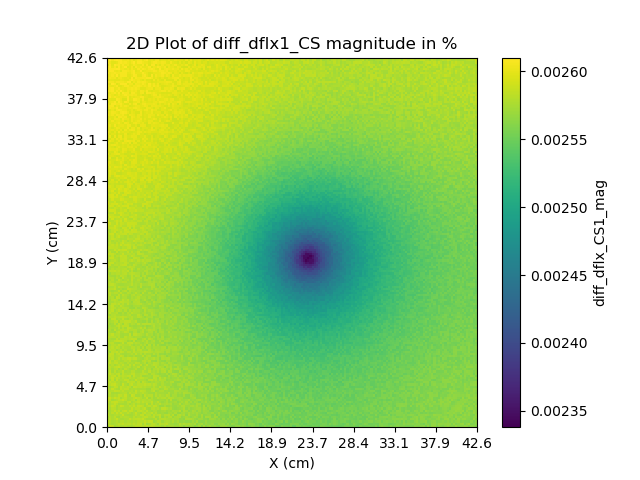
\includegraphics[width=\linewidth]{figures/OBJECTIVES1_TEST02_2DMG_C3_VandV_NOISE_diff_dflx_CS_magnitude_G1.png}
        \end{subfigure}
        \hfill
        \begin{subfigure}{.48\textwidth}
          \centering
          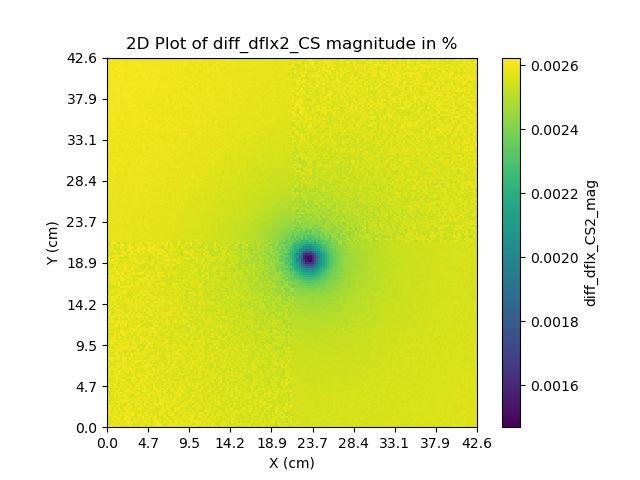
\includegraphics[width=\linewidth]{figures/OBJECTIVES1_TEST02_2DMG_C3_VandV_NOISE_diff_dflx_CS_magnitude_G2.png}
        \end{subfigure}
\end{figure}
\begin{figure}[H]\ContinuedFloat
        \centering
        \begin{subfigure}{.48\textwidth}
          \centering
          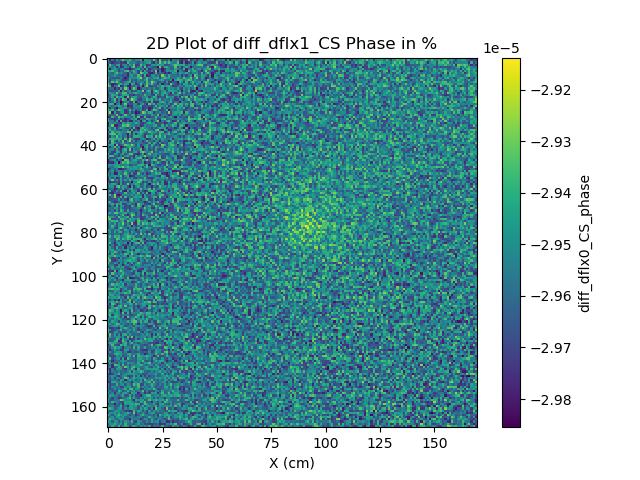
\includegraphics[width=\linewidth]{figures/OBJECTIVES1_TEST02_2DMG_C3_VandV_NOISE_diff_dflx_CS_phase_G1.png}
        \end{subfigure}
        \hfill
        \begin{subfigure}{.48\textwidth}
          \centering
          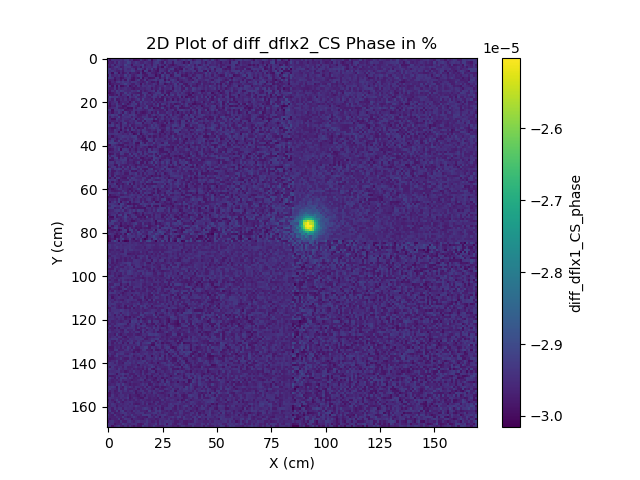
\includegraphics[width=\linewidth]{figures/OBJECTIVES1_TEST02_2DMG_C3_VandV_NOISE_diff_dflx_CS_phase_G2.png}
        \end{subfigure}
        \caption{Difference of neutron noise results between CORE SIM+ and the developed solver}
        \label{fig:C3_noise_results_diff_phi}
\end{figure}

As seen in Figure \ref{fig:C3_noise_results_flx}, Figure \ref{fig:C3_noise_results_phi}, and Figure \ref{fig:C3_noise_results_diff_phi}, the results show that the solutions from the solver agree well with CORE SIM+ solutions. The error is less than 1\% error for the magnitude of the neutron noise, and very low error in the phase of the neutron noise. This shows that the solver works well for 2D rectangular geometries.

\section{3D Westinghouse 4-loop PWR}

In this case, a generic, Western-type PWR is simulated. The overall diameter of the core is 344 cm, and the height of the core is 396.24 cm. This includes the reflector of the core. The active region of the core has a diameter of 322.5 cm and height of 365.76 cm \cite{husseinReactorNeutronNoise2024}. In this case, the simulation includes the reflector regions. It consists of 157 fuel assemblies.

For this case, forward, adjoint, and neutron noise simulations are available in CORE SIM+. These results will be used for comparison. In this dissertation, the forward flux and adjoint flux at the half-plane of the core is compared and reported. For the neutron noise simulation, the plane at which the perturbation happens is reported. The detailed results of the 3D PWR are available in the GitHub repository. The differences between the solver and CORE SIM+ simulation is reported as a relative error defined in Eq. \ref{eq:error1}.

\subsection{Forward Flux Solution}

The forward flux solutions from CORE SIM+, solver, and comparison between the simulators at half-plane ($Z = 27$) are as follows:

\begin{table}[H]
        \centering
        \caption{Eigenvalue comparison of 3D Generic PWR}
        \label{table:PWR3D_fw_results}
        \begin{tabular}{ | M{3.5cm} | M{2cm} | } 
         \hline
         $k_{\text{eff}}$ CORE SIM+ & 1.000965  \\
         \hline
         $k_{\text{eff}}$ solver & 1.000966  \\
         \hline
         Absolute Error (pcm) & 1.0  \\
         \hline
        \end{tabular}
\end{table}

\begin{figure}[H]
        \centering
        \begin{subfigure}{.48\textwidth}
          \centering
          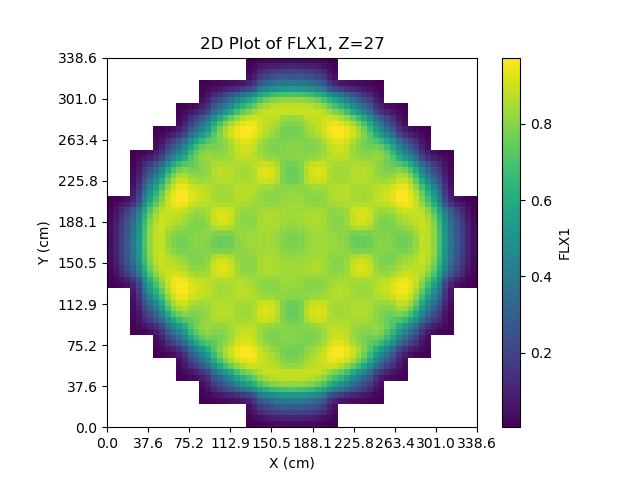
\includegraphics[width=\linewidth]{figures/OBJECTIVES1_TEST06_3DMG_CSTest09_VandV_new_FORWARD_FLX_magnitude_G1_Z27.png}
        \end{subfigure}
        \hfill
        \begin{subfigure}{.48\textwidth}
          \centering
          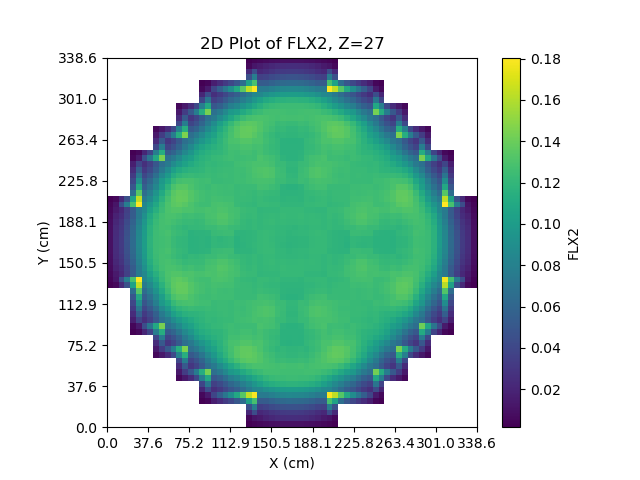
\includegraphics[width=\linewidth]{figures/OBJECTIVES1_TEST06_3DMG_CSTest09_VandV_new_FORWARD_FLX_magnitude_G2_Z27.png}
        \end{subfigure}
        \caption{Forward flux results from CORE SIM+}
        \label{fig:PWR3D_fw_results_flx}
\end{figure}
\begin{figure}[H]
        \centering
        \begin{subfigure}{.48\textwidth}
          \centering
          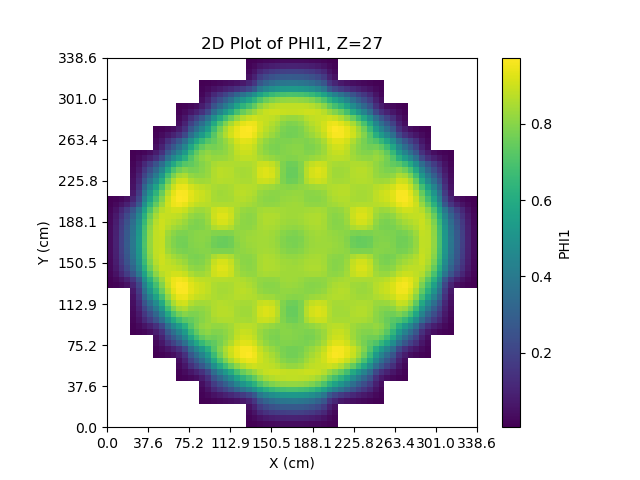
\includegraphics[width=\linewidth]{figures/OBJECTIVES1_TEST06_3DMG_CSTest09_VandV_new_FORWARD_PHI_magnitude_G1_Z27.png}
        \end{subfigure}
        \hfill
        \begin{subfigure}{.48\textwidth}
          \centering
          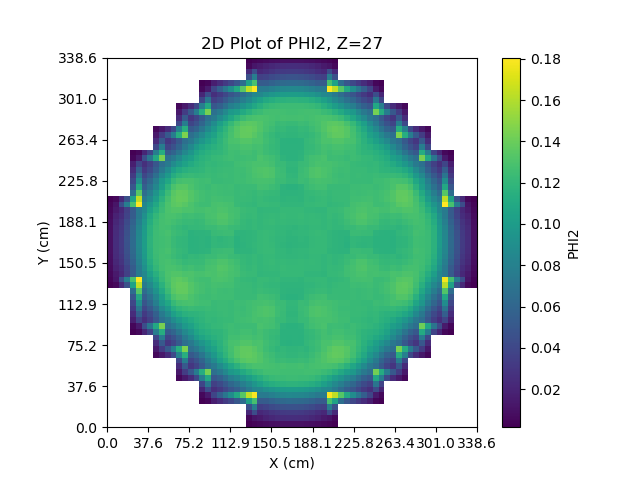
\includegraphics[width=\linewidth]{figures/OBJECTIVES1_TEST06_3DMG_CSTest09_VandV_new_FORWARD_PHI_magnitude_G2_Z27.png}
        \end{subfigure}
        \caption{Forward flux results from the developed solver}
        \label{fig:PWR3D_fw_results_phi}
\end{figure}
\begin{figure}[H]
        \centering
        \begin{subfigure}{.48\textwidth}
          \centering
          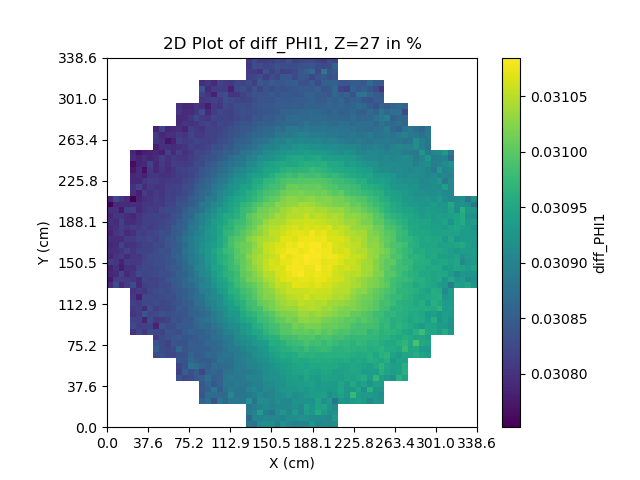
\includegraphics[width=\linewidth]{figures/OBJECTIVES1_TEST06_3DMG_CSTest09_VandV_new_FORWARD_diff_PHI_magnitude_G1_Z27.png}
        \end{subfigure}
        \hfill
        \begin{subfigure}{.48\textwidth}
          \centering
          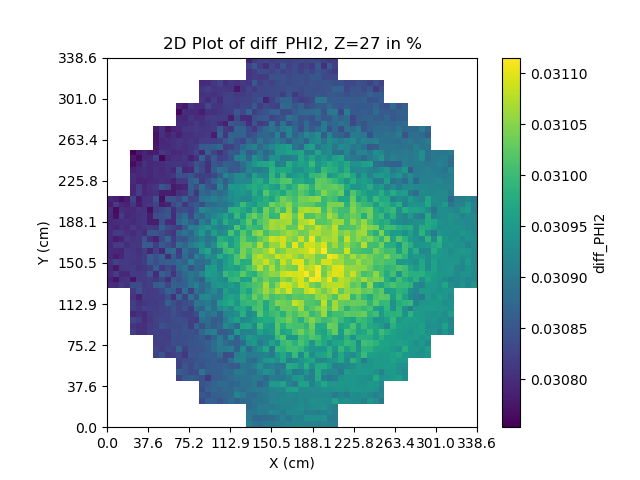
\includegraphics[width=\linewidth]{figures/OBJECTIVES1_TEST06_3DMG_CSTest09_VandV_new_FORWARD_diff_PHI_magnitude_G2_Z27.png}
        \end{subfigure}
        \caption{Difference of forward flux between CORE SIM+ and the solver}
        \label{fig:PWR3D_fw_results_diff_phi}
\end{figure}

The results show that the solver agrees well with CORE SIM+. The $k_{\text{eff}}$ values match between CORE SIM+ and the developed solver with only 1 pcm difference. The error is less than 1\% for the forward flux. This demonstrates that the solver performs effectively for 3D rectangular geometries.

\subsection{Adjoint Flux Solution}

The adjoint flux solutions from CORE SIM+, solver, and comparison between the simulators at half-plane ($Z = 27$) are as follows:

\begin{figure}[H]
        \centering
        \begin{subfigure}{.48\textwidth}
          \centering
          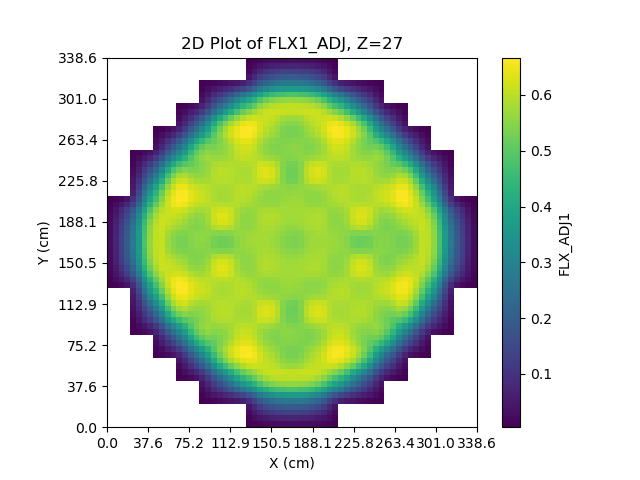
\includegraphics[width=\linewidth]{figures/OBJECTIVES1_TEST06_3DMG_CSTest09_VandV_new_ADJOINT_FLX_ADJ_magnitude_G1_Z27.png}
        \end{subfigure}
        \hfill
        \begin{subfigure}{.48\textwidth}
          \centering
          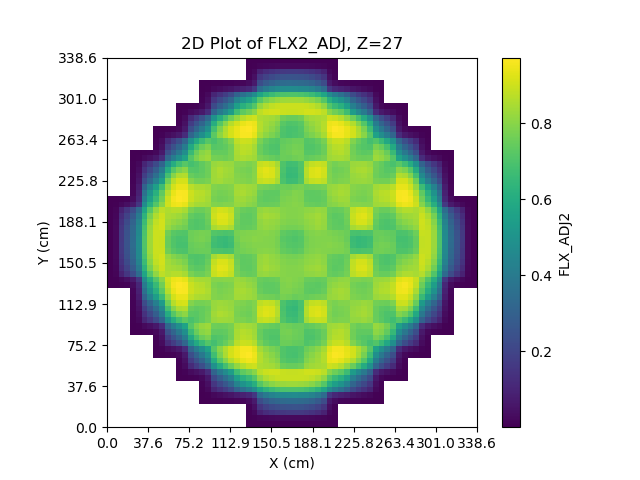
\includegraphics[width=\linewidth]{figures/OBJECTIVES1_TEST06_3DMG_CSTest09_VandV_new_ADJOINT_FLX_ADJ_magnitude_G2_Z27.png}
        \end{subfigure}
        \caption{Adjoint flux results from CORE SIM+}
        \label{fig:PWR3D_adj_results_flx}
\end{figure}
\begin{figure}[H]
        \centering
        \begin{subfigure}{.48\textwidth}
          \centering
          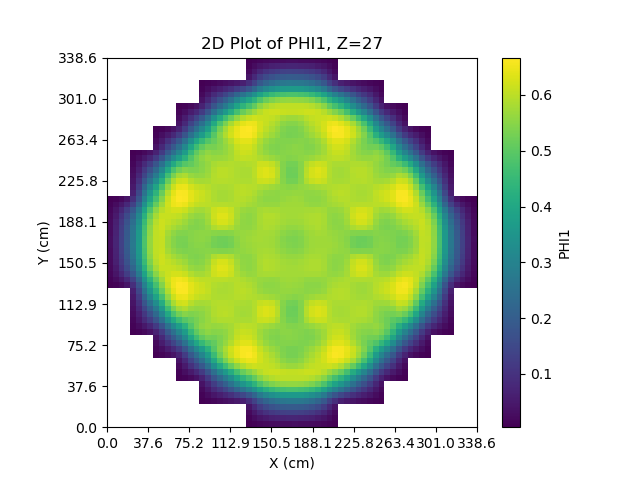
\includegraphics[width=\linewidth]{figures/OBJECTIVES1_TEST06_3DMG_CSTest09_VandV_new_ADJOINT_PHI_magnitude_G1_Z27.png}
        \end{subfigure}
        \hfill
        \begin{subfigure}{.48\textwidth}
          \centering
          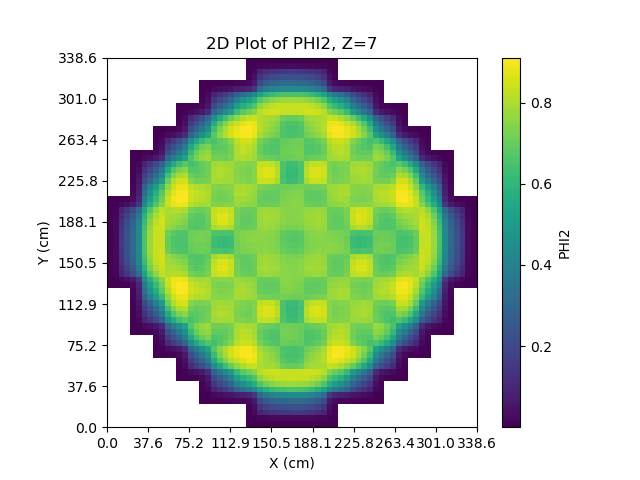
\includegraphics[width=\linewidth]{figures/OBJECTIVES1_TEST06_3DMG_CSTest09_VandV_new_ADJOINT_PHI_magnitude_G2_Z7.png}
        \end{subfigure}
        \caption{Adjoint flux results from the developed solver}
        \label{fig:PWR3D_adj_results_phi}
\end{figure}
\begin{figure}[H]
        \centering
        \begin{subfigure}{.48\textwidth}
          \centering
          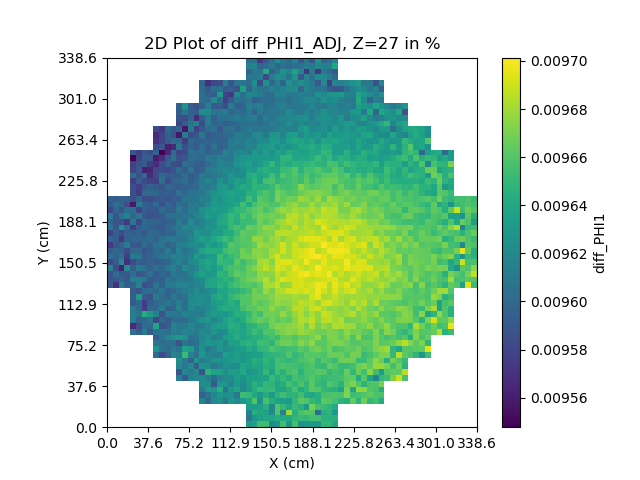
\includegraphics[width=\linewidth]{figures/OBJECTIVES1_TEST06_3DMG_CSTest09_VandV_new_ADJOINT_diff_PHI_magnitude_G1_Z27.png}
        \end{subfigure}
        \hfill
        \begin{subfigure}{.48\textwidth}
          \centering
          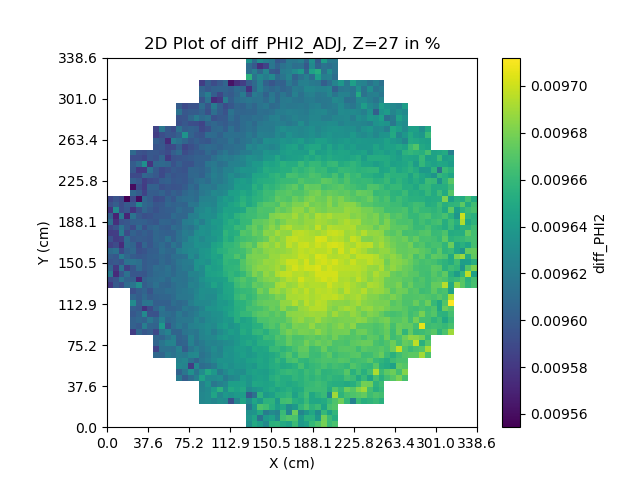
\includegraphics[width=\linewidth]{figures/OBJECTIVES1_TEST06_3DMG_CSTest09_VandV_new_ADJOINT_diff_PHI_magnitude_G2_Z27.png}
        \end{subfigure}
        \caption{Difference of adjoint flux between CORE SIM+ and the solver}
        \label{fig:PWR3D_adj_results_diff_phi}
\end{figure}

The results show that the solver agrees well with CORE SIM+. The error is less than 1\% for the adjoint flux. This indicates that the solver works well for 3D rectangular geometries.

\subsection{Neutron Noise Solution}

In this case, the noise source is defined as a point source at $Z = 10$. Specifically, the noise source is defined as follows:
\begin{equation}
    \delta \Sigma_{t,2}(12, 25, 10, \omega) = 0.05 \Sigma_{t,2} (12, 25, 10)
\end{equation}

This means that the noise source is defined as 5\% perturbation of the thermal total cross sections from their steady state value. The value (12,25,10) indicates the ($x,y,z$) component of the noise source. The neutron noise solutions from CORE SIM+, the developed solver, and the comparison between them at Z=10 are as follows:

\begin{figure}[H]
        \centering
        \begin{subfigure}{.48\textwidth}
          \centering
          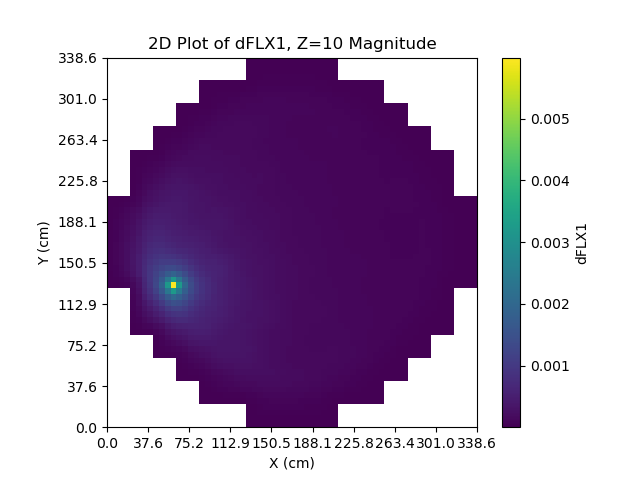
\includegraphics[width=\linewidth]{figures/OBJECTIVES1_TEST06_3DMG_CSTest09_VandV_new_NOISE_dFLX_magnitude_G1_Z10.png}
        \end{subfigure}
        \hfill
        \begin{subfigure}{.48\textwidth}
          \centering
          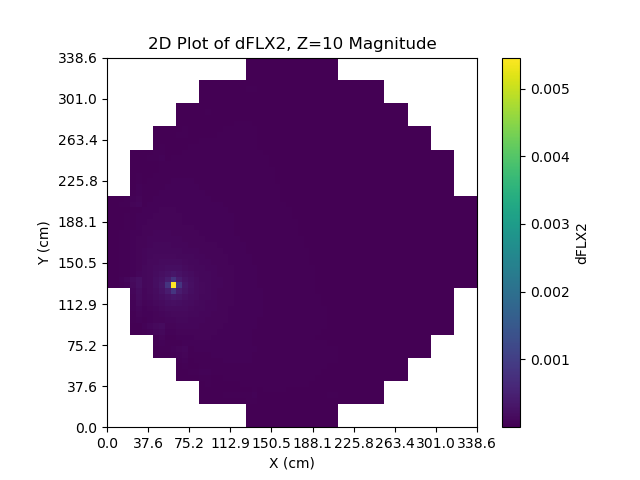
\includegraphics[width=\linewidth]{figures/OBJECTIVES1_TEST06_3DMG_CSTest09_VandV_new_NOISE_dFLX_magnitude_G2_Z10.png}
        \end{subfigure}
\end{figure}
\begin{figure}[H]\ContinuedFloat
        \centering
        \begin{subfigure}{.48\textwidth}
          \centering
          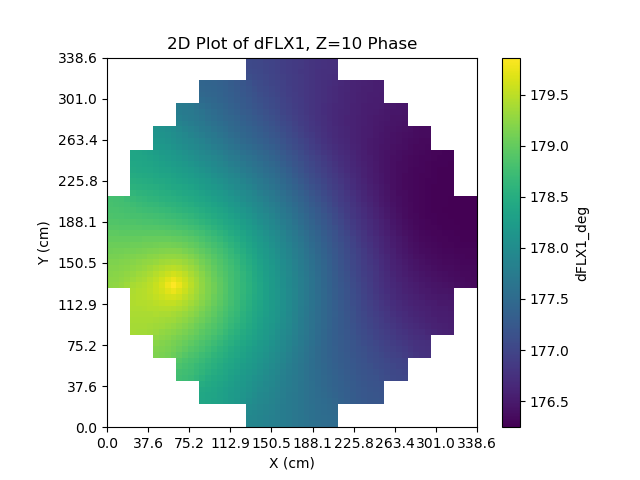
\includegraphics[width=\linewidth]{figures/OBJECTIVES1_TEST06_3DMG_CSTest09_VandV_new_NOISE_dFLX_phase_G1_Z10.png}
        \end{subfigure}
        \hfill
        \begin{subfigure}{.48\textwidth}
          \centering
          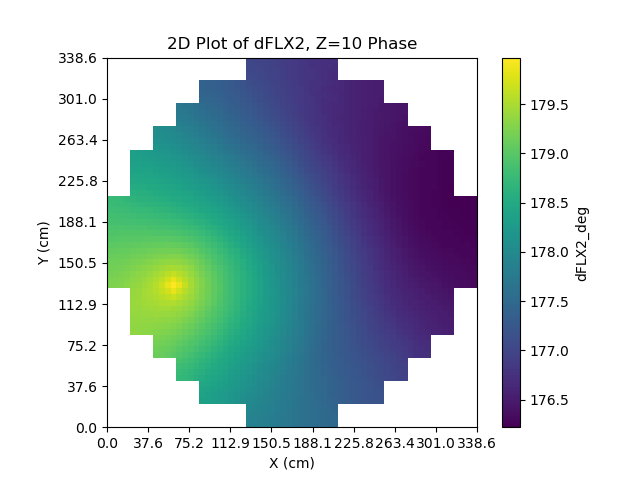
\includegraphics[width=\linewidth]{figures/OBJECTIVES1_TEST06_3DMG_CSTest09_VandV_new_NOISE_dFLX_phase_G2_Z10.png}
        \end{subfigure}
        \caption{Neutron noise results from CORE SIM+}
        \label{fig:PWR3D_noise_results_flx}
\end{figure}

\newpage
\begin{figure}[H]
        \centering
        \begin{subfigure}{.48\textwidth}
          \centering
          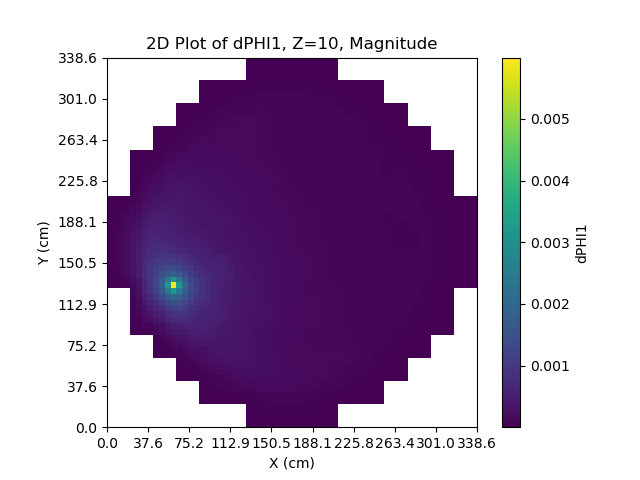
\includegraphics[width=\linewidth]{figures/OBJECTIVES1_TEST06_3DMG_CSTest09_VandV_new_NOISE_dPHI_magnitude_G1_Z10.png}
        \end{subfigure}
        \hfill
        \begin{subfigure}{.48\textwidth}
          \centering
          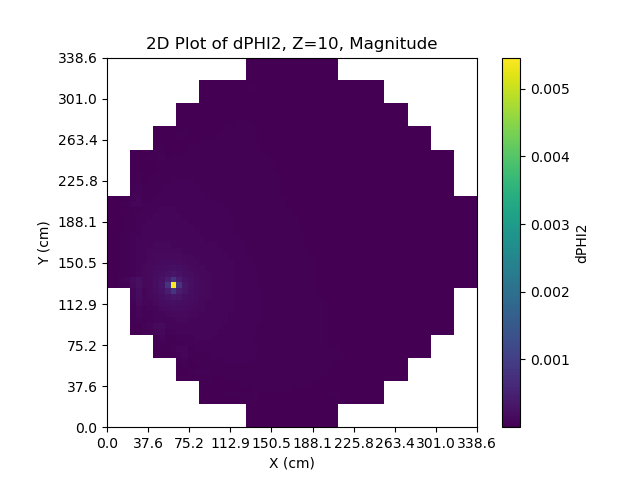
\includegraphics[width=\linewidth]{figures/OBJECTIVES1_TEST06_3DMG_CSTest09_VandV_new_NOISE_dPHI_magnitude_G2_Z10.png}
        \end{subfigure}
\end{figure}
\begin{figure}[H]\ContinuedFloat
        \centering
        \begin{subfigure}{.48\textwidth}
          \centering
          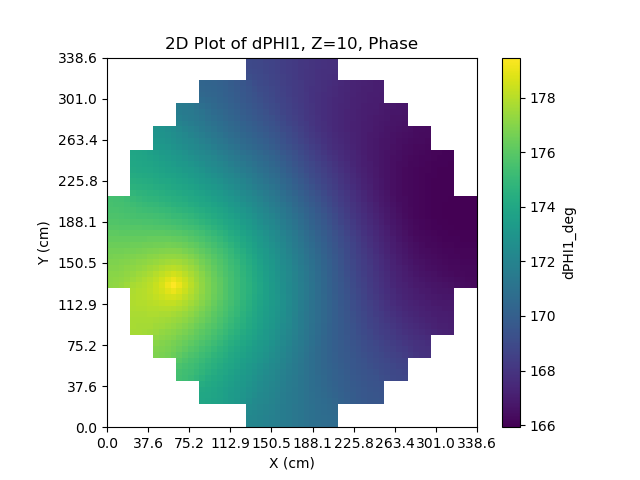
\includegraphics[width=\linewidth]{figures/OBJECTIVES1_TEST06_3DMG_CSTest09_VandV_new_NOISE_dPHI_phase_G1_Z10.png}
        \end{subfigure}
        \hfill
        \begin{subfigure}{.48\textwidth}
          \centering
          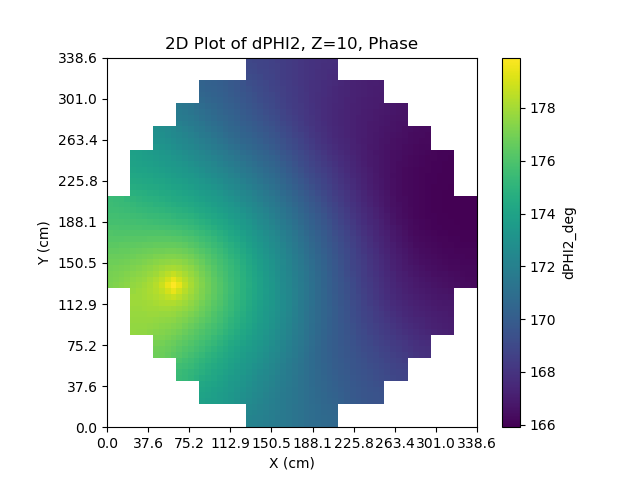
\includegraphics[width=\linewidth]{figures/OBJECTIVES1_TEST06_3DMG_CSTest09_VandV_new_NOISE_dPHI_phase_G2_Z10.png}
        \end{subfigure}
        \caption{Neutron noise results from the developed solver}
        \label{fig:PWR3D_noise_results_phi}
\end{figure}

\newpage
\begin{figure}[H]
        \centering
        \begin{subfigure}{.48\textwidth}
          \centering
          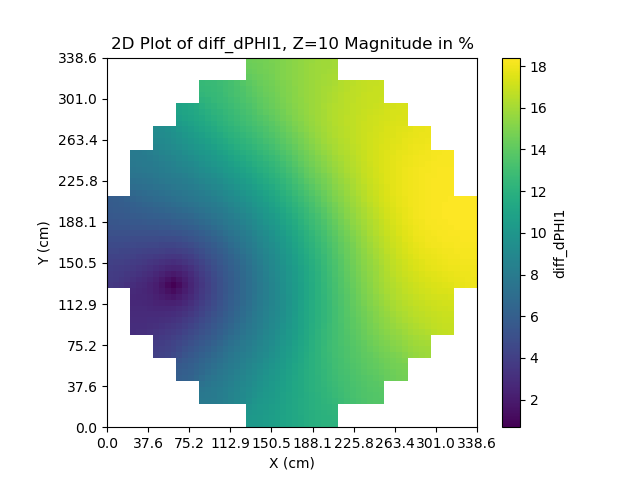
\includegraphics[width=\linewidth]{figures/OBJECTIVES1_TEST06_3DMG_CSTest09_VandV_new_NOISE_diff_dPHI_magnitude_G1_Z10.png}
        \end{subfigure}
        \hfill
        \begin{subfigure}{.48\textwidth}
          \centering
          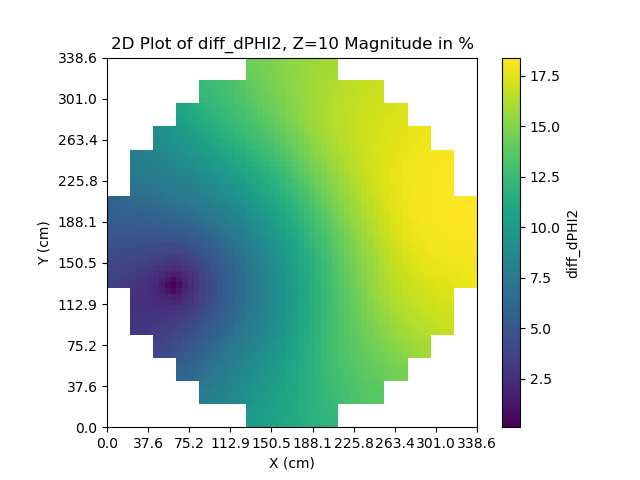
\includegraphics[width=\linewidth]{figures/OBJECTIVES1_TEST06_3DMG_CSTest09_VandV_new_NOISE_diff_dPHI_magnitude_G2_Z10.png}
        \end{subfigure}
\end{figure}
\begin{figure}[H]\ContinuedFloat
        \centering
        \begin{subfigure}{.48\textwidth}
          \centering
          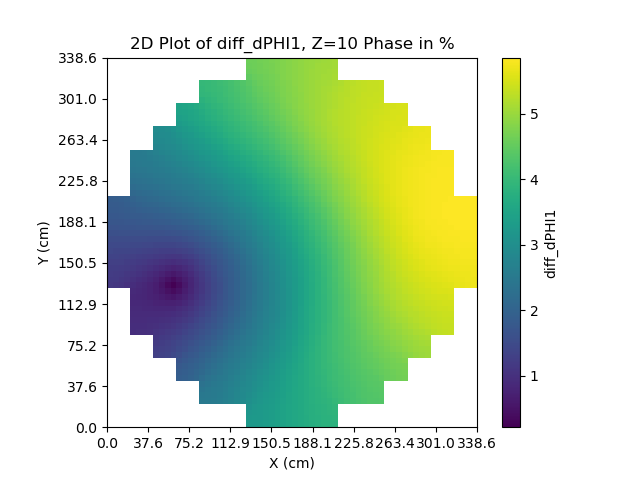
\includegraphics[width=\linewidth]{figures/OBJECTIVES1_TEST06_3DMG_CSTest09_VandV_new_NOISE_diff_dPHI_phase_G1_Z10.png}
        \end{subfigure}
        \hfill
        \begin{subfigure}{.48\textwidth}
          \centering
          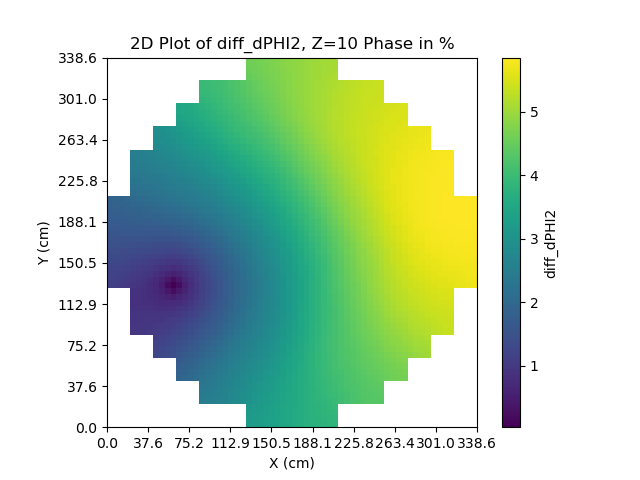
\includegraphics[width=\linewidth]{figures/OBJECTIVES1_TEST06_3DMG_CSTest09_VandV_new_NOISE_diff_dPHI_phase_G2_Z10.png}
        \end{subfigure}
        \caption{Difference of neutron noise results between CORE SIM+ and the developed solver}
        \label{fig:PWR3D_noise_results_diff_phi}
\end{figure}

The results show that the solutions generated by the solver agree well with those from CORE SIM+. The error is higher at the periphery for the magnitude of the neutron noise, and a maximum of 5\% for the phase of the neutron noise. The increase of error in the periphery is caused by the fact that the neutron noise in the periphery is close to zero. As a result, even small absolute deviations in the reconstructed flux can lead to disproportionately large relative errors. In general, the overall results show that the solver works well for 3D rectangular geometries.

\section{2D BIBLIS Benchmark}

The 2D BIBLIS Benchmark, referred to the first nuclear power plant build in the municipality of Biblis (Germany), is is a realistic and highly non-separable 2-group problem representative of an actual operating pressurized water reactor (PWR) with a checker-board-loaded core \cite{mullerBenchmarkingMultigroupDiffusion1991}. The homogenized fuel assemblies with widths of 23.1226 cm and seven different compositions are present in the core which is surrounded by a 23.1226 cm homogenized reflector (i.e. the baffle is bomogenized with the water reflector) with vacuum external boundary conditions. The particular configuration used in this work is that corresponding to the "rods out" case for which the cross section data were taken from a paper by \cite{hebertApplicationHermiteMethod1985}. A complete description of this problem is provided in Figure \ref{fig:2DBIBLIS} and Table \ref{table:2DBIBLISXS}. 

\begin{figure}[H]
        \centering
        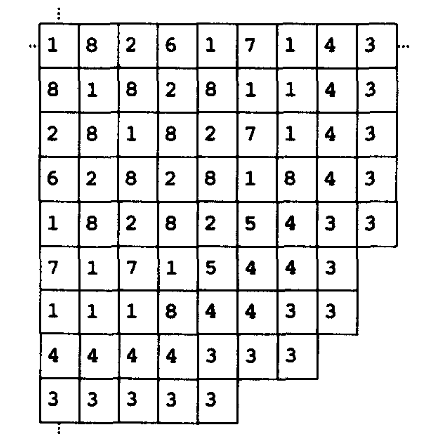
\includegraphics[width=0.45\textwidth]{figures/2DBIBLIS.png}
        \caption{Quarter core configuration of 2D BIBLIS Benchmark (obtained from \cite{mullerBenchmarkingMultigroupDiffusion1991})}
        \label{fig:2DBIBLIS}
\end{figure}

\begin{table}[H]
        \centering
        \caption{Homogenized cross-section data of 2D BIBLIS Benchmark (obtained from \cite{mullerBenchmarkingMultigroupDiffusion1991})}
        \label{table:2DBIBLISXS}
        \begin{tabular}{ | M{1.5cm} | M{1cm} | M{1.5cm} | M{1.5cm} | M{1.5cm} | M{1.5cm} | M{1.5cm} | } 
         \hline
         \textbf{Material} & \textbf{Group} & \textbf{$D_g$} ($cm$) & \textbf{$\Sigma_{a,g}$} ($cm^{-1}$) & \textbf{$\nu \Sigma_{f,g}$}  ($cm^{-1}$) & \textbf{$\Sigma_{f,g}$}  ($cm^{-1}$) & \textbf{$\Sigma_{s,1 \rightarrow}$}  ($cm^{-1}$)\\
         \hline
         \multirow{2}{*}{1} & 1 & 1.4360 & 0.0095042 & 0.0058708 & 0.0023768 & \\
         \cline{2-7}        & 2 & 0.3635 & 0.0750580 & 0.0960670 & 0.0388940 & 0.017754 \\
         \hline
         \multirow{2}{*}{2} & 1 & 1.4366 & 0.0096785 & 0.0061908 & 0.0025064 & \\
         \cline{2-7}        & 2 & 0.3636 & 0.0784360 & 0.1035800 & 0.0419350 & 0.017621 \\
         \hline
         \multirow{2}{*}{3} & 1 & 1.3200 & 0.0026562 & 0.0000000 & 0.0000000 & \\
         \cline{2-7}        & 2 & 0.2772 & 0.0715960 & 0.0000000 & 0.0000000 & 0.023106 \\
         \hline
         \multirow{2}{*}{4} & 1 & 1.4389 & 0.0103630 & 0.0074527 & 0.0030173 & \\
         \cline{2-7}        & 2 & 0.3638 & 0.0914080 & 0.1323600 & 0.0535870 & 0.017101 \\
         \hline
         \multirow{2}{*}{5} & 1 & 1.4381 & 0.0100030 & 0.0061908 & 0.0025064 & \\
         \cline{2-7}        & 2 & 0.3665 & 0.0848280 & 0.1035800 & 0.0419350 & 0.017192 \\
         \hline
         \multirow{2}{*}{6} & 1 & 1.4385 & 0.0101320 & 0.0064285 & 0.0026026 & \\
         \cline{2-7}        & 2 & 0.3665 & 0.0873140 & 0.1091100 & 0.0441740 & 0.017192 \\
         \hline
         \multirow{2}{*}{7} & 1 & 1.4389 & 0.0101650 & 0.0061908 & 0.0025064 & \\
         \cline{2-7}        & 2 & 0.3679 & 0.0880240 & 0.1035800 & 0.0419350 & 0.017125 \\
         \hline
         \multirow{2}{*}{8} & 1 & 1.4393 & 0.0102940 & 0.0064285 & 0.0026026 & \\
         \cline{2-7}        & 2 & 0.3680 & 0.0905100 & 0.1091100 & 0.0441740 & 0.017027 \\
         \hline
        \end{tabular}
\end{table}

The 2D BIBLIS Benchmark has been simulated in FEMFFUSION \cite{vidal-ferrandizFEMFFUSIONFiniteElement2023} and compared with the developed solver. The results are as follows:

\subsection{Forward Simulation}
\begin{table}[H]
        \centering
        \caption{Eigenvalue comparison of 2D BIBLIS Benchmark}
        \label{table:BIBLIS_fw_results}
        \begin{tabular}{ | M{3.5cm} | M{2cm} | } 
         \hline
         $k_{\text{eff}}$ FEMFFUSION & 1.02535  \\
         \hline
         $k_{\text{eff}}$ solver & 1.02519  \\
         \hline
         Absolute Error (pcm) & 16.0  \\
         \hline
        \end{tabular}
\end{table}

\begin{figure}[H]
        \centering
        \begin{subfigure}{.48\textwidth}
          \centering
          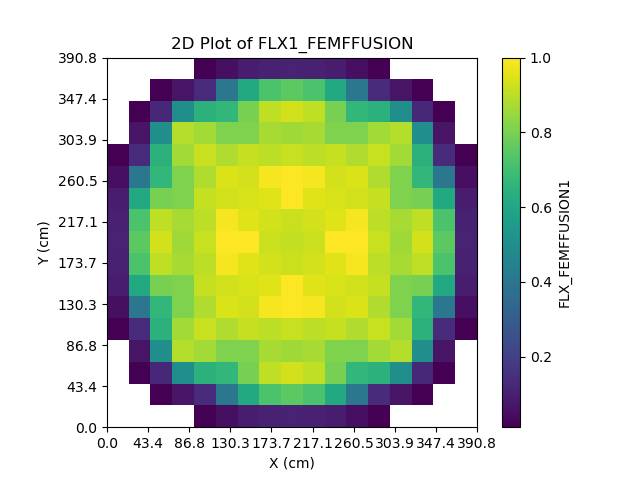
\includegraphics[width=\linewidth]{figures/OBJECTIVES1_TEST03_2DMG_BIBLIS_VandV_FORWARD_FLX_FEMFFUSION_G1.png}
        \end{subfigure}
        \hfill
        \begin{subfigure}{.48\textwidth}
          \centering
          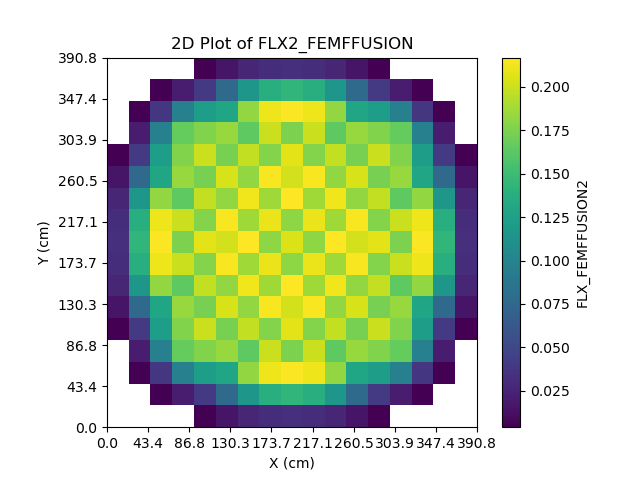
\includegraphics[width=\linewidth]{figures/OBJECTIVES1_TEST03_2DMG_BIBLIS_VandV_FORWARD_FLX_FEMFFUSION_G2.png}
        \end{subfigure}
        \caption{Forward flux results from FEMFFUSION}
        \label{fig:BIBLIS_fw_results_flx}
\end{figure}
\begin{figure}[H]
        \centering
        \begin{subfigure}{.48\textwidth}
          \centering
          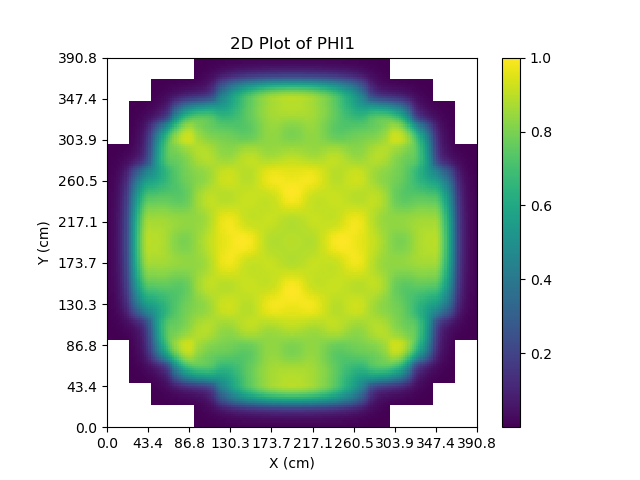
\includegraphics[width=\linewidth]{figures/OBJECTIVES1_TEST03_2DMG_BIBLIS_VandV_FORWARD_PHI_G1.png}
        \end{subfigure}
        \hfill
        \begin{subfigure}{.48\textwidth}
          \centering
          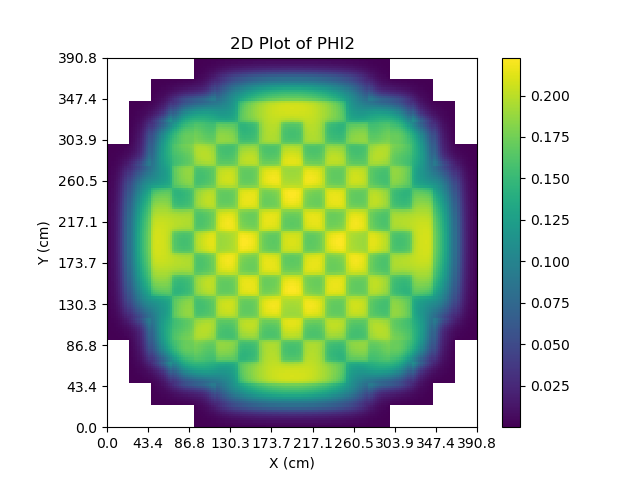
\includegraphics[width=\linewidth]{figures/OBJECTIVES1_TEST03_2DMG_BIBLIS_VandV_FORWARD_PHI_G2.png}
        \end{subfigure}
        \caption{Forward flux results from the developed solver}
        \label{fig:BIBLIS_fw_results_phi}
\end{figure}
\begin{figure}[H]
        \centering
        \begin{subfigure}{.48\textwidth}
          \centering
          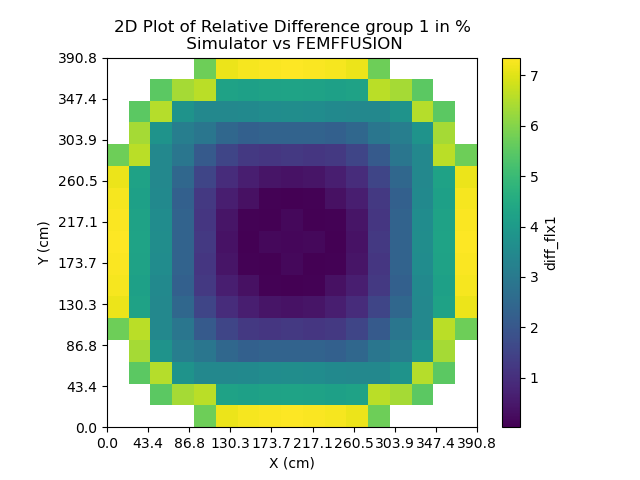
\includegraphics[width=\linewidth]{figures/OBJECTIVES1_TEST03_2DMG_BIBLIS_VandV_FORWARD_diff_flx_G1.png}
        \end{subfigure}
        \hfill
        \begin{subfigure}{.48\textwidth}
          \centering
          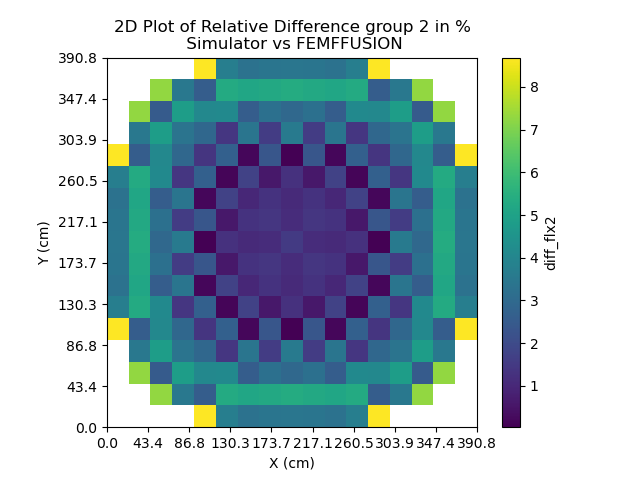
\includegraphics[width=\linewidth]{figures/OBJECTIVES1_TEST03_2DMG_BIBLIS_VandV_FORWARD_diff_flx_G2.png}
        \end{subfigure}
        \caption{Difference of forward flux between FEMFFUSION and the solver}
\end{figure}

The forward results show that some discrepancies are observed between the developed solver and FEMFFUSION. This difference is due to the use of the finite element method in FEMFFUSION, which has different degrees of accuracy compared to the box-scheme finite difference used in the solver. The error in $k_\text{eff}$ is 16 pcm and the maximum error in the neutron flux is about 8\%. Considering this difference in spatial discretization method, the solver generally works well and in a certain degree of agreement with FEMFFUSION.

\subsection{Adjoint Simulation}

\begin{figure}[H]
        \centering
        \begin{subfigure}{.48\textwidth}
          \centering
          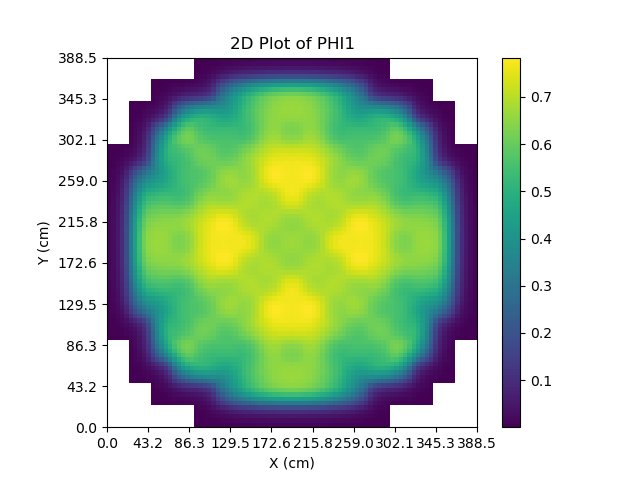
\includegraphics[width=\linewidth]{figures/OBJECTIVES1_TEST03_2DMG_BIBLIS_VandV_ADJOINT_PHI_G1.png}
        \end{subfigure}
        \hfill
        \begin{subfigure}{.48\textwidth}
          \centering
          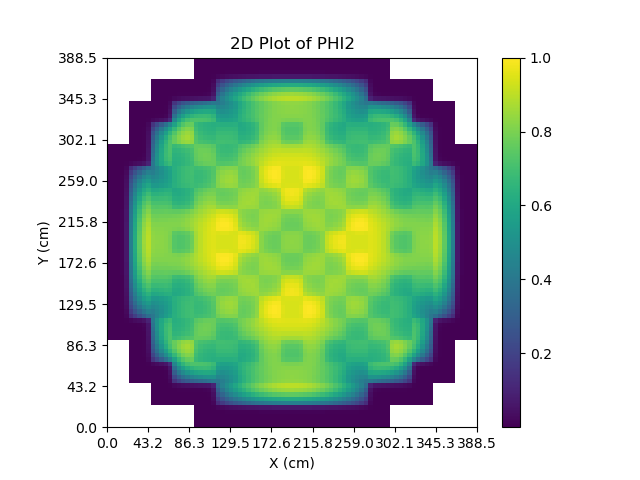
\includegraphics[width=\linewidth]{figures/OBJECTIVES1_TEST03_2DMG_BIBLIS_VandV_ADJOINT_PHI_G2.png}
        \end{subfigure}
        \caption{Adjoint flux results from the developed solver}
        \label{fig:BIBLIS_adj_results_phi}
\end{figure}

There are no direct comparisons available for the adjoint flux solution. However, the results of the adjoint simulation show expected results using the developed solver, with the maximum flux at the thermal group solution. 

\subsection{Neutron Noise Simulation}

For the neutron noise simulation, the noise source is defined as an AVS-type noise source located at the center of the core. The noise sources are defined as follows:
\begin{equation}
    \begin{aligned}
        \delta \Sigma_{a,1} (\textbf{r}_p) &= 0.005 \\
        \delta \Sigma_{a,2} (\textbf{r}_p) &= 0.005 \\
        \delta \Sigma_{s,1\rightarrow2} (\textbf{r}_p) &= 0.005 \\        
    \end{aligned}
\end{equation}

The 2D BIBLIS Benchmark has been simulated in FEMFFUSION \cite{vidal-ferrandizFEMFFUSIONFiniteElement2023} and compared with the developed solver. The results are as follows:

\begin{figure}[H]
        \centering
        \begin{subfigure}{.48\textwidth}
          \centering
          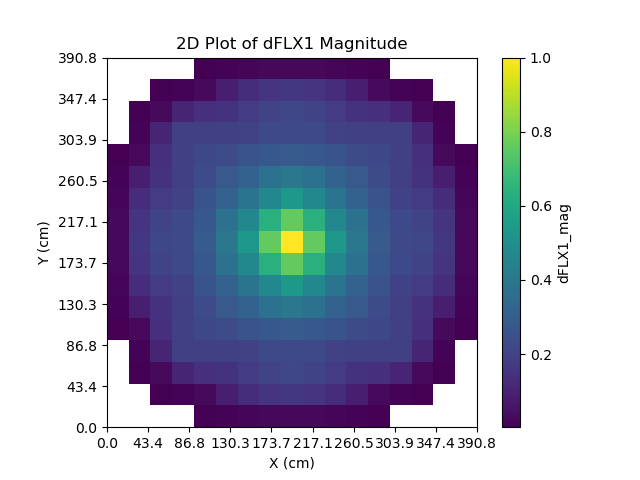
\includegraphics[width=\linewidth]{figures/OBJECTIVES1_TEST03_2DMG_BIBLIS_VandV_NOISE_dFLX_magnitude_G1.png}
        \end{subfigure}
        \hfill
        \begin{subfigure}{.48\textwidth}
          \centering
          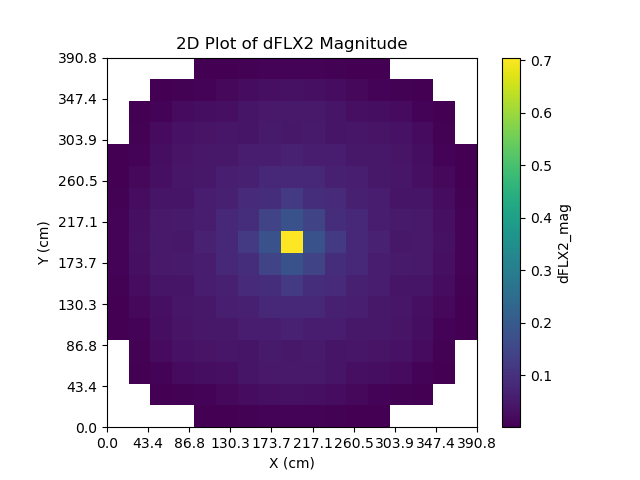
\includegraphics[width=\linewidth]{figures/OBJECTIVES1_TEST03_2DMG_BIBLIS_VandV_NOISE_dFLX_magnitude_G2.png}
        \end{subfigure}
\end{figure}
\begin{figure}[H]\ContinuedFloat
        \centering
        \begin{subfigure}{.48\textwidth}
          \centering
          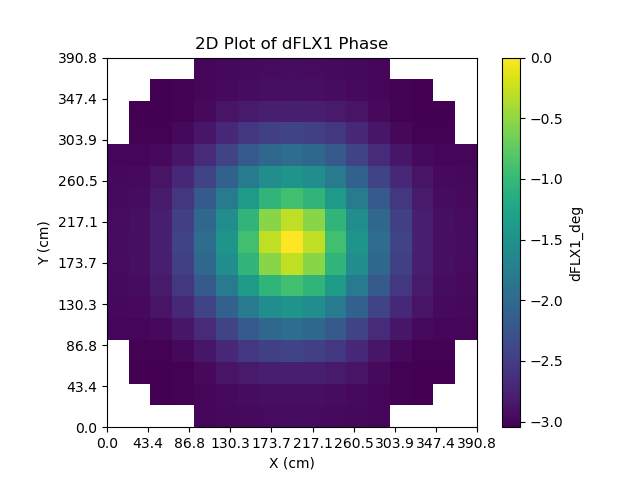
\includegraphics[width=\linewidth]{figures/OBJECTIVES1_TEST03_2DMG_BIBLIS_VandV_NOISE_dFLX_phase_G1.png}
        \end{subfigure}
        \hfill
        \begin{subfigure}{.48\textwidth}
          \centering
          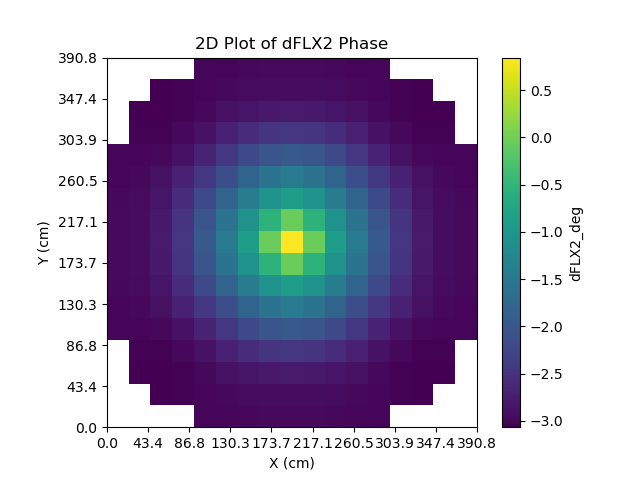
\includegraphics[width=\linewidth]{figures/OBJECTIVES1_TEST03_2DMG_BIBLIS_VandV_NOISE_dFLX_phase_G2.png}
        \end{subfigure}
        \caption{Neutron noise results from FEMFFUSION}
        \label{fig:BIBLIS_noise_results_flx}
\end{figure}

\begin{figure}[H]
        \centering
        \begin{subfigure}{.48\textwidth}
          \centering
          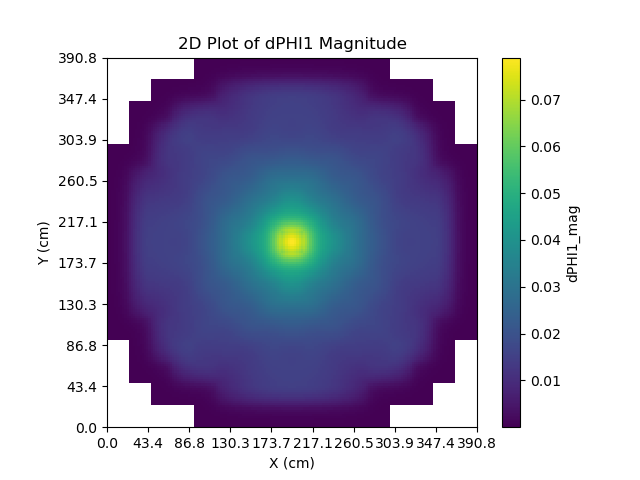
\includegraphics[width=\linewidth]{figures/OBJECTIVES1_TEST03_2DMG_BIBLIS_VandV_NOISE_dPHI_magnitude_G1.png}
        \end{subfigure}
        \hfill
        \begin{subfigure}{.48\textwidth}
          \centering
          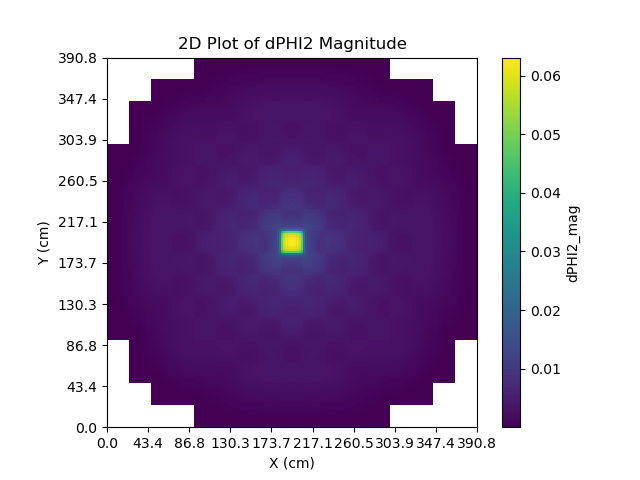
\includegraphics[width=\linewidth]{figures/OBJECTIVES1_TEST03_2DMG_BIBLIS_VandV_NOISE_dPHI_magnitude_G2.png}
        \end{subfigure}
\end{figure}
\begin{figure}[H]\ContinuedFloat
        \centering
        \begin{subfigure}{.48\textwidth}
          \centering
          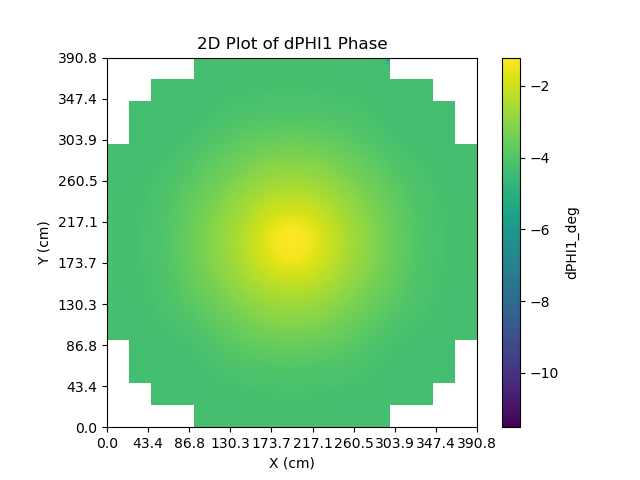
\includegraphics[width=\linewidth]{figures/OBJECTIVES1_TEST03_2DMG_BIBLIS_VandV_NOISE_dPHI_phase_G1.png}
        \end{subfigure}
        \hfill
        \begin{subfigure}{.48\textwidth}
          \centering
          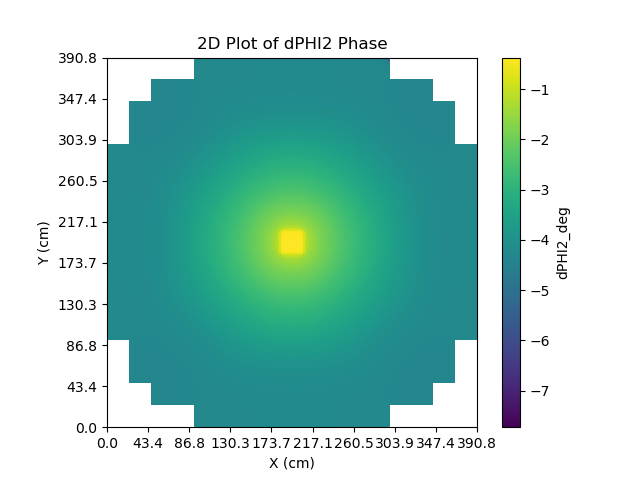
\includegraphics[width=\linewidth]{figures/OBJECTIVES1_TEST03_2DMG_BIBLIS_VandV_NOISE_dPHI_phase_G2.png}
        \end{subfigure}
        \caption{Neutron noise results from the developed solver}
        \label{fig:BIBLIS_noise_results_phi}
\end{figure}

\newpage
\begin{figure}[H]
        \centering
        \begin{subfigure}{.48\textwidth}
          \centering
          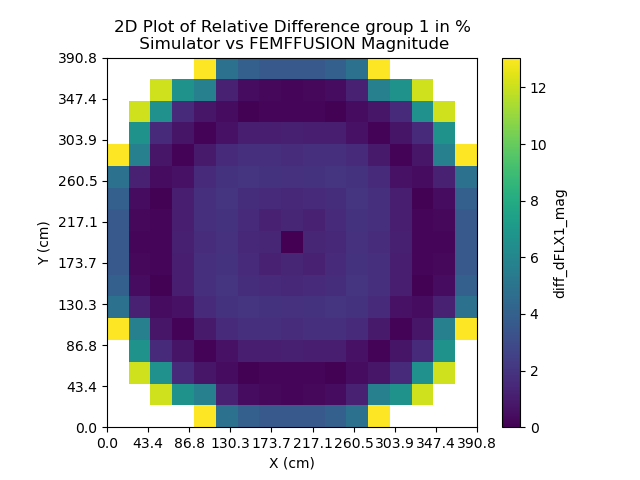
\includegraphics[width=\linewidth]{figures/OBJECTIVES1_TEST03_2DMG_BIBLIS_VandV_NOISE_diff_dFLX_magnitude_G1.png}
        \end{subfigure}
        \hfill
        \begin{subfigure}{.48\textwidth}
          \centering
          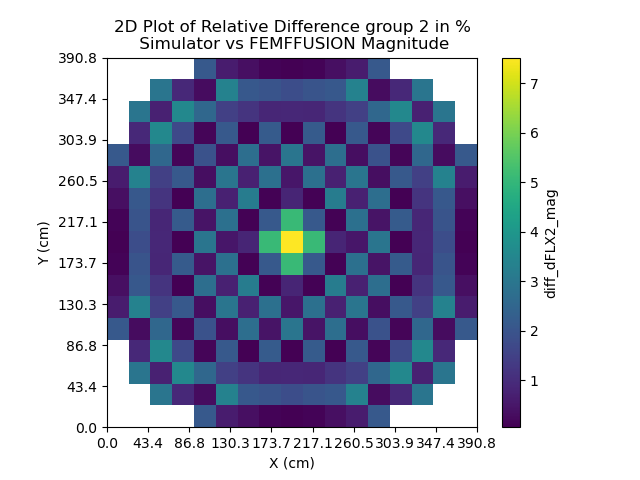
\includegraphics[width=\linewidth]{figures/OBJECTIVES1_TEST03_2DMG_BIBLIS_VandV_NOISE_diff_dFLX_magnitude_G2.png}
        \end{subfigure}
\end{figure}
\begin{figure}[H]\ContinuedFloat
        \centering
        \begin{subfigure}{.48\textwidth}
          \centering
          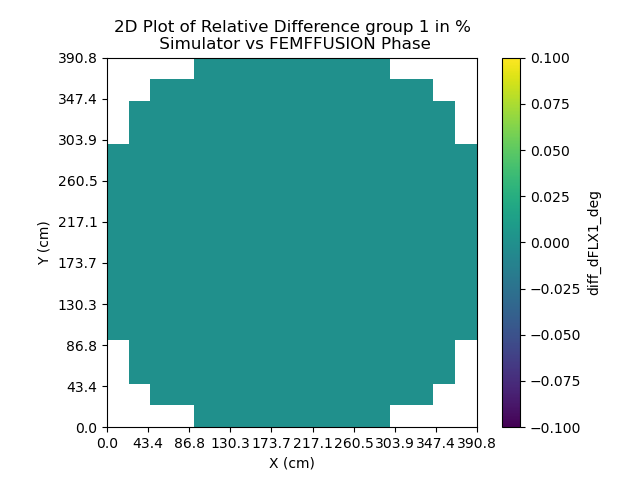
\includegraphics[width=\linewidth]{figures/OBJECTIVES1_TEST03_2DMG_BIBLIS_VandV_NOISE_diff_dFLX_phase_G1.png}
        \end{subfigure}
        \hfill
        \begin{subfigure}{.48\textwidth}
          \centering
          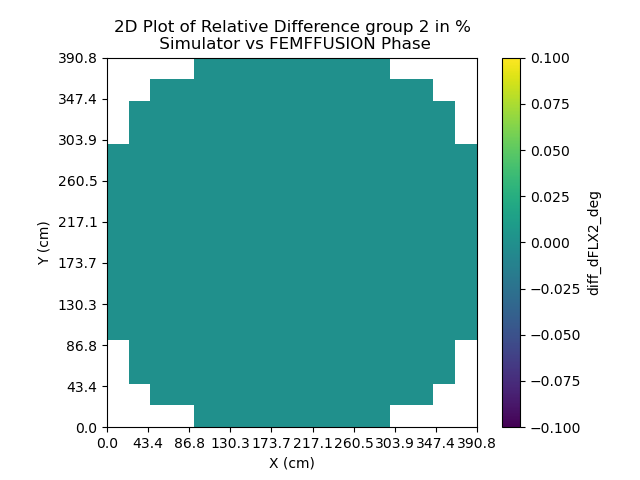
\includegraphics[width=\linewidth]{figures/OBJECTIVES1_TEST03_2DMG_BIBLIS_VandV_NOISE_diff_dFLX_phase_G2.png}
        \end{subfigure}
        \caption{Difference of neutron noise results between FEMFFUSION and the developed solver}
        \label{fig:BIBLIS_noise_results_diff_phi}
\end{figure}

Comparing the results between FEMFFUSION and the developed solver, the results show that the neutron noise solution between FEMFFUSION and the developed solver are in good agreement to each other. The maximum error of the magnitude is about 12\% and it is mainly located at the periphery of the core. Considering this difference in spatial discretization method, the solver generally works well and in a certain degree of agreement with FEMFFUSION.

\section{2D VVER-400}

\subsection{Neutron Noise Solution}

In this case, it is defined that the noise source perturbed the thermal total cross-section.
\begin{equation}
    \delta \Sigma_{t,2}(\textbf{r}_p,\omega) = 0.05 \Sigma_{t,2}(\textbf{r}_p)
\end{equation}
where we define $\textbf{r}_p$ near the center of the core, indicated by yellow hexagon in Figure \ref{fig:2DVVER_source}.
\begin{figure}[H]
        \centering
        \begin{subfigure}{.48\textwidth}
          \centering
          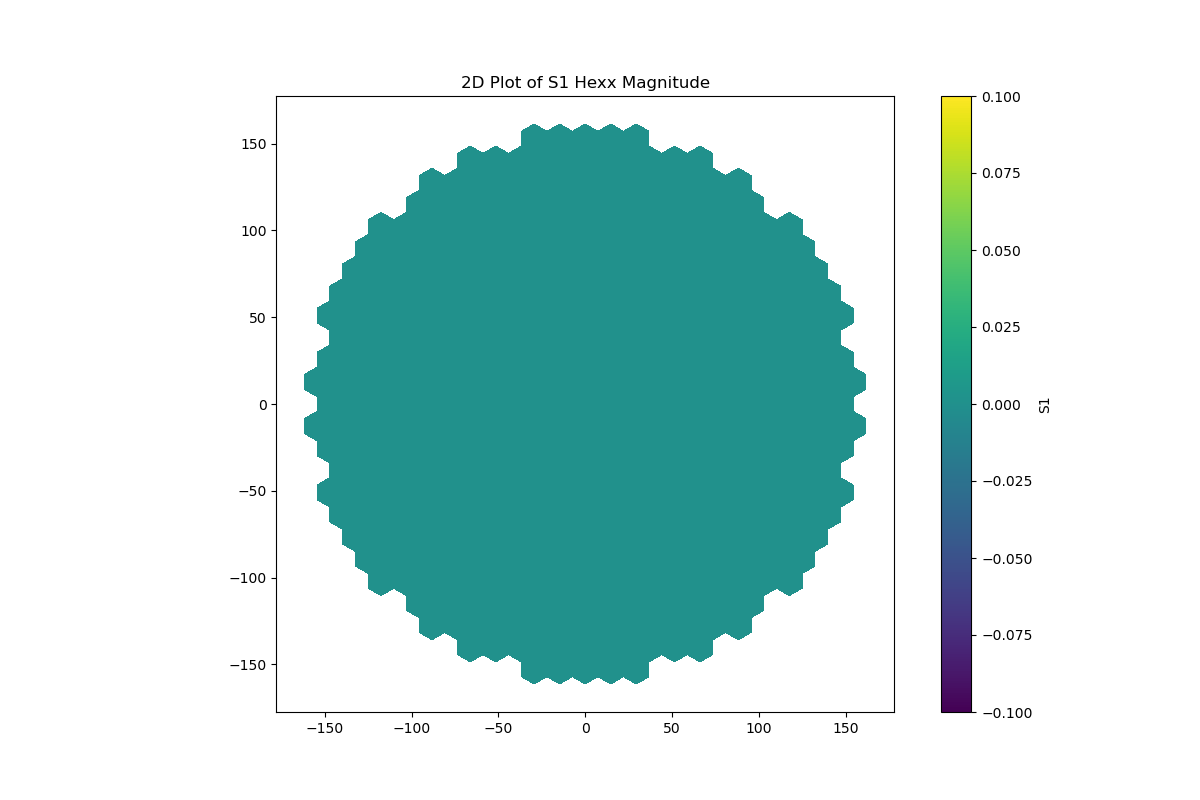
\includegraphics[width=\linewidth]{figures/OBJECTIVES1_TEST05_2DTriMG_VVER400_VandV_level2_NOISE_S_magnitude_G1.png}
        \end{subfigure}
        \hfill
        \begin{subfigure}{.48\textwidth}
          \centering
          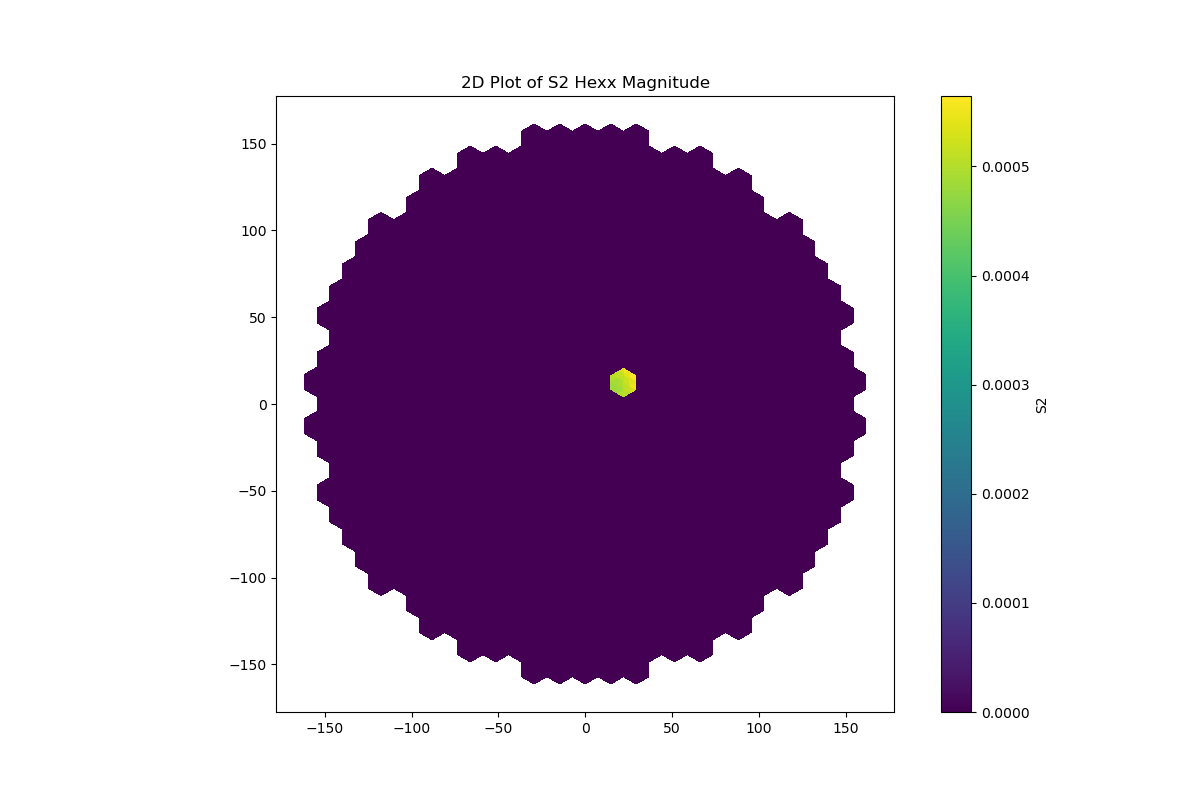
\includegraphics[width=\linewidth]{figures/OBJECTIVES1_TEST05_2DTriMG_VVER400_VandV_level2_NOISE_S_magnitude_G2.png}
        \end{subfigure}
        \caption{Noise source location for 2D VVER-400}
        \label{fig:2DVVER_source}
\end{figure}
The simulation is done at frequency of 1 Hz. There is no comparison for this simulation. The results of neutron noise simulations are described in Figure 

\begin{figure}[H]
        \centering
        \begin{subfigure}{.48\textwidth}
          \centering
          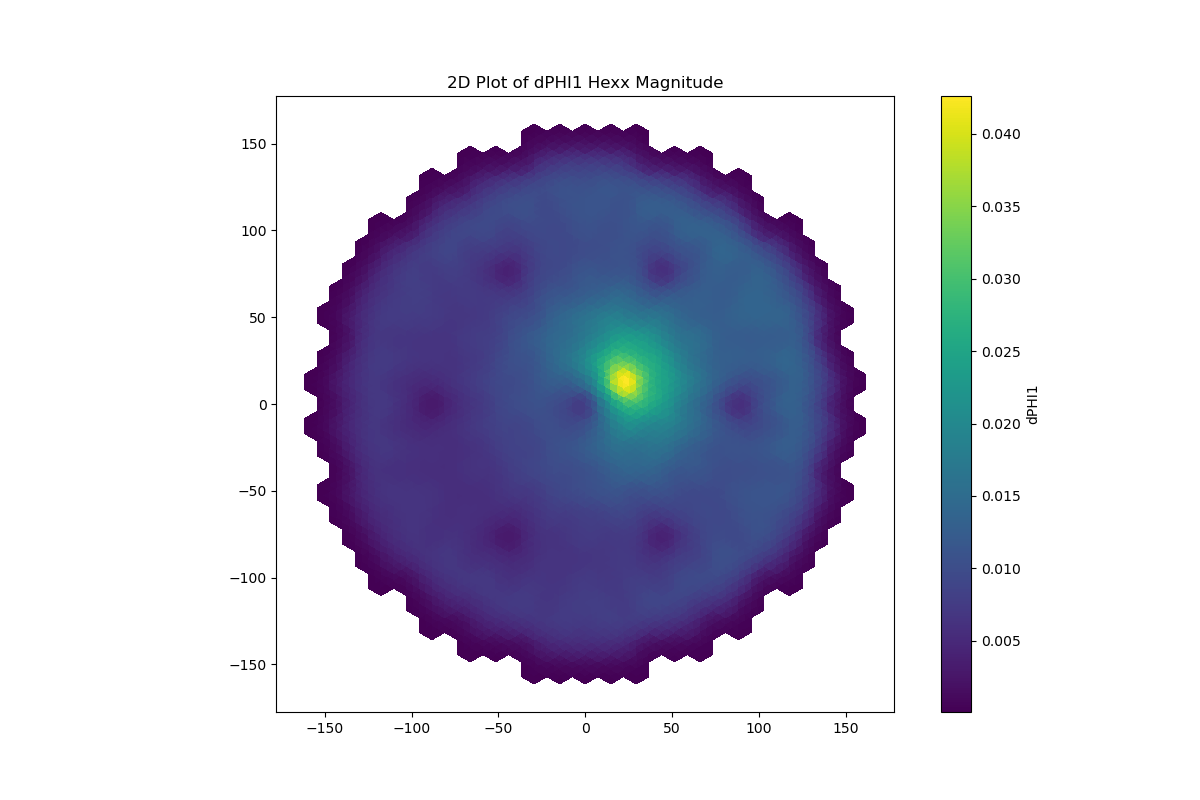
\includegraphics[width=\linewidth]{figures/OBJECTIVES1_TEST05_2DTriMG_VVER400_VandV_level2_NOISE_dPHI_magnitude_G1.png}
        \end{subfigure}
        \hfill
        \begin{subfigure}{.48\textwidth}
          \centering
          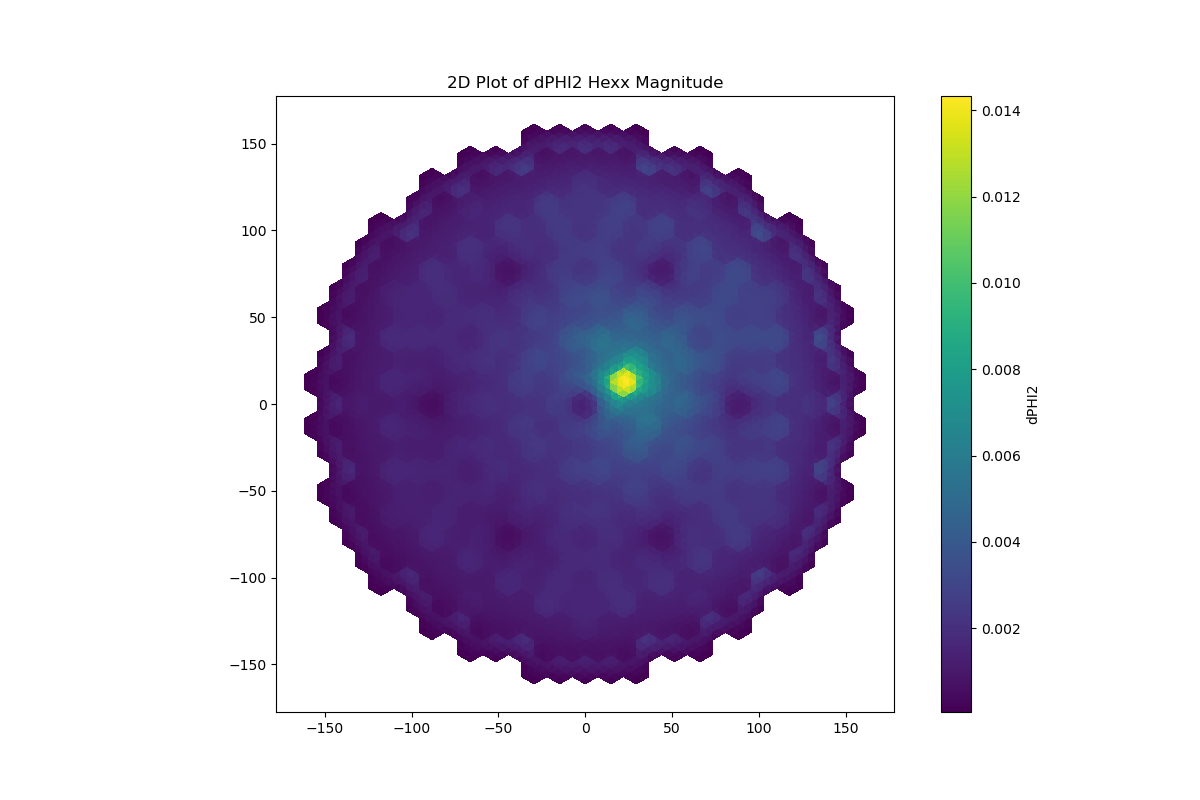
\includegraphics[width=\linewidth]{figures/OBJECTIVES1_TEST05_2DTriMG_VVER400_VandV_level2_NOISE_dPHI_magnitude_G2.png}
        \end{subfigure}
\end{figure}
\begin{figure}[H]\ContinuedFloat
        \centering
        \begin{subfigure}{.48\textwidth}
          \centering
          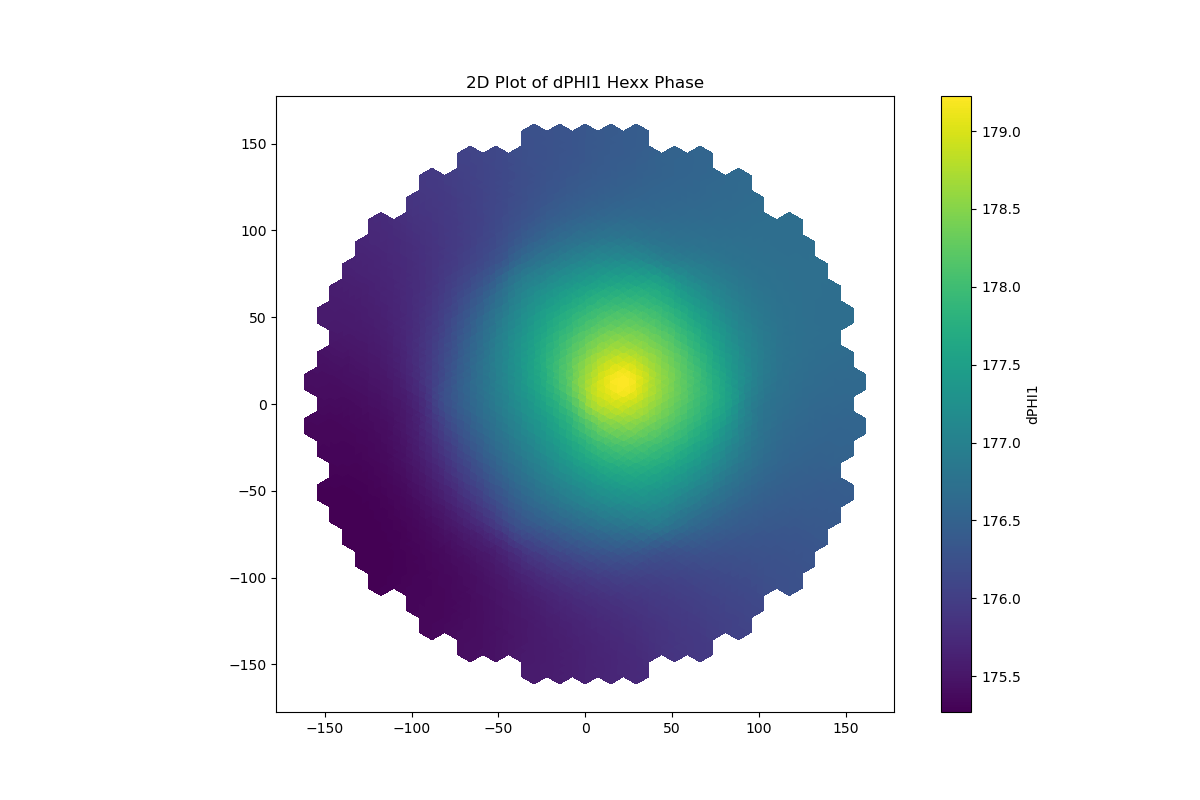
\includegraphics[width=\linewidth]{figures/OBJECTIVES1_TEST05_2DTriMG_VVER400_VandV_level2_NOISE_dPHI_phase_G1.png}
        \end{subfigure}
        \hfill
        \begin{subfigure}{.48\textwidth}
          \centering
          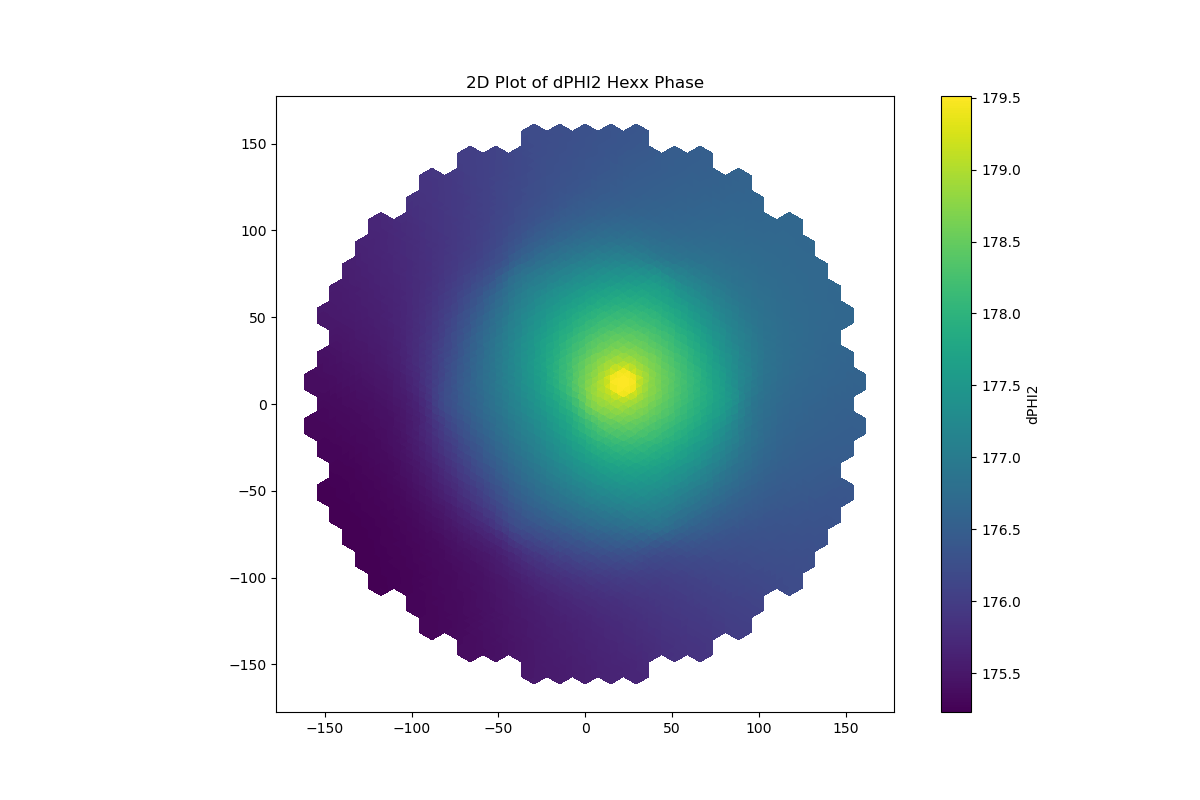
\includegraphics[width=\linewidth]{figures/OBJECTIVES1_TEST05_2DTriMG_VVER400_VandV_level2_NOISE_dPHI_phase_G2.png}
        \end{subfigure}
        \caption{Neutron noise results from the developed tool}
        \label{fig:2DVVER_noise_results}
\end{figure}

The results show that magnitude of the peak fast neutron noise is larger than the thermal neutron noise. However, the fast neutron noise is more dispersed than the thermal neutron noise. The phase plot shows similarities between fast and thermal group.

\section{3D Langenbuch (LMW) Benchmark}

\subsection{Forward Simulation}

The LMW Benchmark is a two-group, six-delayed neutron precursor families and 3D time-dependent reactor benchmark without thermal-hydraulic feedback. The reactor was developed and studied by \cite{langenbuchCoarseMeshFluxExpansionMethod1977}. The reactor consists of 77 fuel assembly 40 reflector assemblies. The size of each assembly is 20 cm $\times$ 20 cm. The zero flux boundary condition is used in this case. This case has been used to verify transient solvers due to its fast resolution \cite{vidal-ferrandizFEMFFUSIONFiniteElement2023}. The core configuration and the material cross sections are defined in Figure \ref{fig:3DLangenbuch}, Table \ref{table:3DLangenbuchXS}, and Table \ref{table:3DLangenbuchKin}. 

\begin{figure}[H]
        \centering
        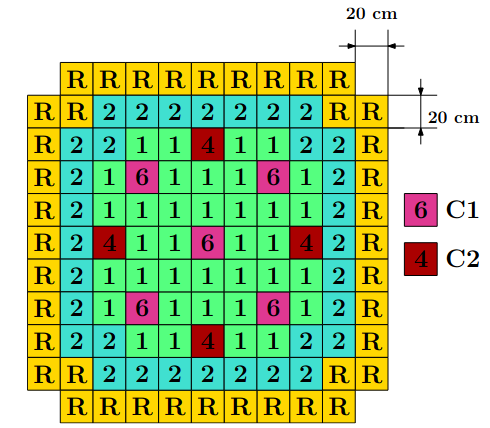
\includegraphics[width=0.45\textwidth]{figures/3DLangenbuch.png}
        \caption{Core configuration of 3D Langenbuch Benchmark (obtained from \cite{vidal-ferrandizFEMFFUSIONFiniteElement2023})}
        \label{fig:3DLangenbuch}
\end{figure}

\begin{table}[H]
        \centering
        \caption{Homogenized cross-section of 3D Langenbuch Benchmark (obtained from \cite{vidal-ferrandizFEMFFUSIONFiniteElement2023})}
        \label{table:3DLangenbuchXS}
        \begin{tabular}{ | M{4.5cm} | M{1cm} | M{1.5cm} | M{2cm} | M{2cm} | M{2cm} | } 
         \hline
         \textbf{Material} & \textbf{Group} & \textbf{$D_g$} ($cm$) & \textbf{$\Sigma_{a,g}$} ($cm^{-1}$) & \textbf{$\nu \Sigma_{f,g}$}  ($cm^{-1}$) & \textbf{$\Sigma_{s,1 \rightarrow}$}  ($cm^{-1}$)\\
         \hline
         \multirow{2}{*}{1 - Fuel} & 1 & 1.423913 & 0.010402060 & 0.006477691 & \\
         \cline{2-6}               & 2 & 0.356306 & 0.087662170 & 0.112732800 & 0.01755550 \\
         \hline
         \multirow{2}{*}{2 - Fuel} & 1 & 1.425611 & 0.010992630 & 0.007503284 & \\
         \cline{2-6}               & 2 & 0.350574 & 0.099256340 & 0.137800400 & 0.01717768 \\
         \hline
         \multirow{2}{*}{R - Reflector} & 1 & 1.634227 & 0.002660573 & 0.000000000 & \\
         \cline{2-6}                    & 2 & 0.264002 & 0.049363510 & 0.000000000 & 0.02759693 \\
         \hline
         \multirow{2}{*}{4 \& 6 - Absorbent} & 1 & 1.423913 & 0.010952060 & 0.006477691 & \\
         \cline{2-6}                         & 2 & 0.356306 & 0.091462170 & 0.112732800 & 0.01755550 \\
         \hline
         \multirow{2}{*}{5 - Reflector + Absorbent} & 1 & 1.634227 & 0.00321020 & 0.000000000 & \\
         \cline{2-6}                                & 2 & 0.264002 & 0.05316351 & 0.000000000 & 0.02759693 \\
         \hline
        \end{tabular}
\end{table}

\begin{table}[H]
        \centering
        \caption{Neutron precursors data of 3D Langenbuch Benchmark (obtained from \cite{vidal-ferrandizFEMFFUSIONFiniteElement2023})}
        \label{table:3DLangenbuchKin}
        \begin{tabular}{ | M{2.5cm} | M{1.5cm} | M{1.5cm} | M{1.5cm} | M{1.5cm} | M{1.5cm} |  M{1.5cm} |} 
         \hline
         \textbf{Group (k)} & \textbf{1} & \textbf{2} & \textbf{3} & \textbf{4} & \textbf{5} & \textbf{6} \\
         \hline
         $\beta_k$                & 0.000247 & 0.0013845 & 0.001222 & 0.0026455 & 0.000832 & 0.000169 \\
         \hline
         $\lambda_k^d$ ($s^{-1}$) & 0.0127 & 0.0317 & 0.115 & 0.311 & 1.4 & 3.87 \\
         \hline
        \end{tabular}
\end{table}

The forward simulation of the 3D Langenbuch Benchmark has been simulated in FEMFFUSION \cite{vidal-ferrandizFEMFFUSIONFiniteElement2023} and compared with the developed solver. The results are as follows:

\begin{table}[H]
        \centering
        \caption{Eigenvalue results of 3D Langenbuch (LMW) Benchmark}
        \label{table:LMW_fw_results}
        \begin{tabular}{ | M{3.5cm} | M{2cm} | } 
         \hline
         $k_{\text{eff}}$ FEMFFUSION & 0.999748   \\
         \hline
         $k_{\text{eff}}$ solver & 1.000866  \\
         \hline
         Absolute Error (pcm) & 111.8  \\
         \hline
        \end{tabular}
\end{table}

\begin{figure}[H]
        \centering
        \begin{subfigure}{.48\textwidth}
          \centering
          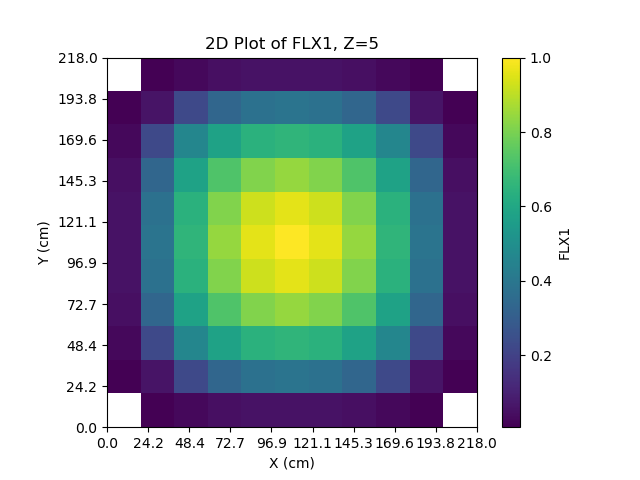
\includegraphics[width=\linewidth]{figures/OBJECTIVES1_TEST10_3DMG_Langenbuch_FORWARD_FLX_G1_Z5.png}
        \end{subfigure}
        \hfill
        \begin{subfigure}{.48\textwidth}
          \centering
          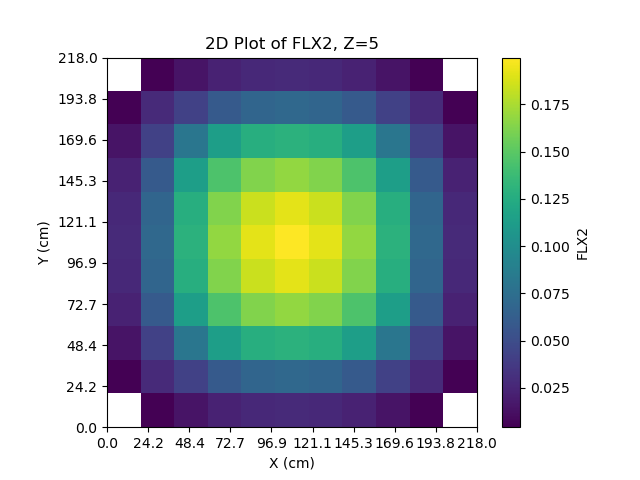
\includegraphics[width=\linewidth]{figures/OBJECTIVES1_TEST10_3DMG_Langenbuch_FORWARD_FLX_G2_Z5.png}
        \end{subfigure}
        \caption{Forward flux results from FEMFFUSION at midplane (Z=5)}
        \label{fig:LMW_fw_results_flx}
\end{figure}
\begin{figure}[H]
        \centering
        \begin{subfigure}{.48\textwidth}
          \centering
          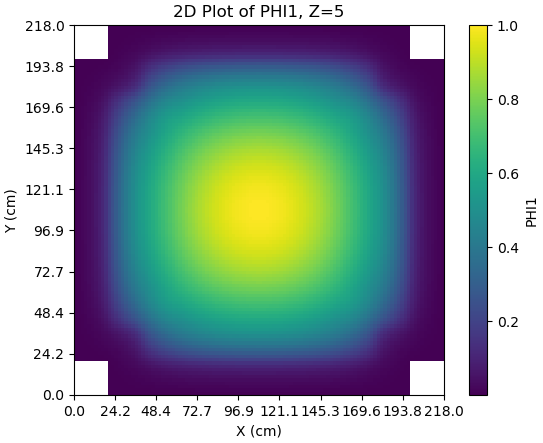
\includegraphics[width=\linewidth]{figures/OBJECTIVES1_TEST10_3DMG_Langenbuch_FORWARD_PHI_magnitude_G1_Z5.png}
        \end{subfigure}
        \hfill
        \begin{subfigure}{.48\textwidth}
          \centering
          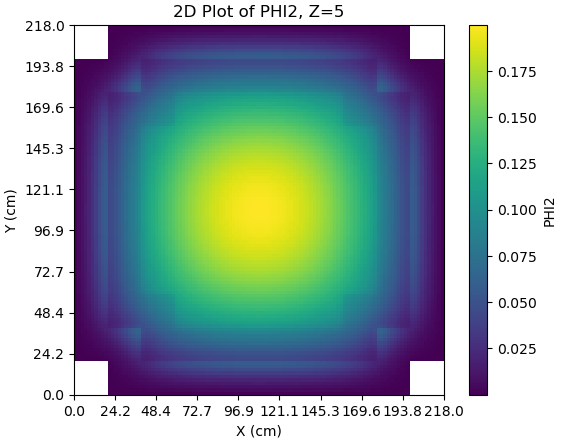
\includegraphics[width=\linewidth]{figures/OBJECTIVES1_TEST10_3DMG_Langenbuch_FORWARD_PHI_magnitude_G2_Z5.png}
        \end{subfigure}
        \caption{Forward flux results from the developed solver at midplane (Z=5)}
        \label{fig:LMW_fw_results_phi}
\end{figure}
\begin{figure}[H]
        \centering
        \begin{subfigure}{.48\textwidth}
          \centering
          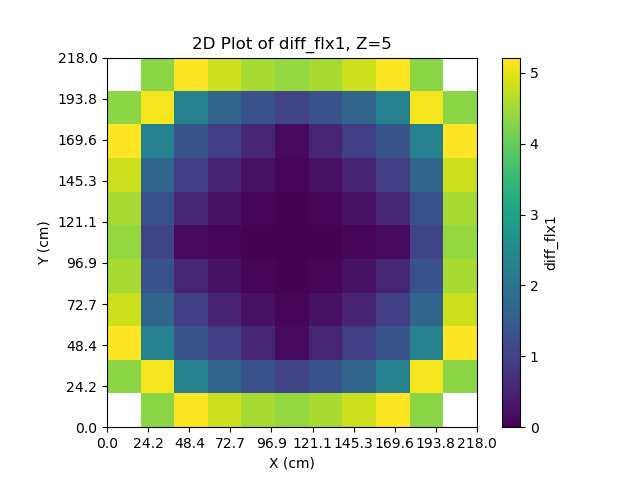
\includegraphics[width=\linewidth]{figures/OBJECTIVES1_TEST10_3DMG_Langenbuch_FORWARD_diff_flx_G1_Z5.png}
        \end{subfigure}
        \hfill
        \begin{subfigure}{.48\textwidth}
          \centering
          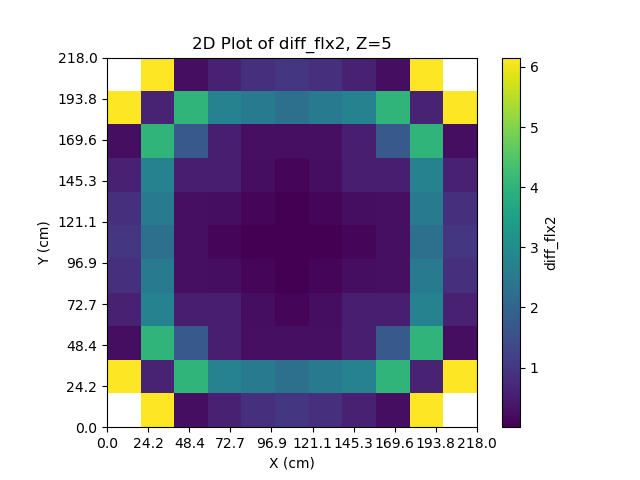
\includegraphics[width=\linewidth]{figures/OBJECTIVES1_TEST10_3DMG_Langenbuch_FORWARD_diff_flx_G2_Z5.png}
        \end{subfigure}
        \caption{Difference of forward flux between FEMFFUSION and the solver at midplane (Z=5)}
\end{figure}

The forward results show that some discrepancies are observed between the developed solver and FEMFFUSION. The difference in $k_\text{eff}$ is 111.8 pcm and the maximum error of forward flux at midplane is about 6\%. This difference is due to the use of the finite element method in FEMFFUSION, which has different degrees of accuracy compared to the box-scheme finite difference used in the solver. Considering this difference in spatial discretization method, the solver generally works well and in a certain degree of agreement with FEMFFUSION.

\subsection{Neutron Noise Simulation}

For the neutron noise simulation, the noise source is defined as an AVS-type noise source location $\textbf{r}_p$ is at the center of the core and midplane ($Z=5$). The noise sources are defined as follows:
\begin{equation}
    \begin{aligned}
        \delta \Sigma_{t,2} (\textbf{r}_p, \omega) &= 0.05 \Sigma_{t,2} (\textbf{r}_p)\\    
    \end{aligned}
\end{equation}

There is no comparison for this simulation. The results of the simulations at the midplane are described in Figure \ref{fig:Langenbuch_noise_results}.
\newpage
\begin{figure}[H]
        \centering
        \begin{subfigure}{.48\textwidth}
          \centering
          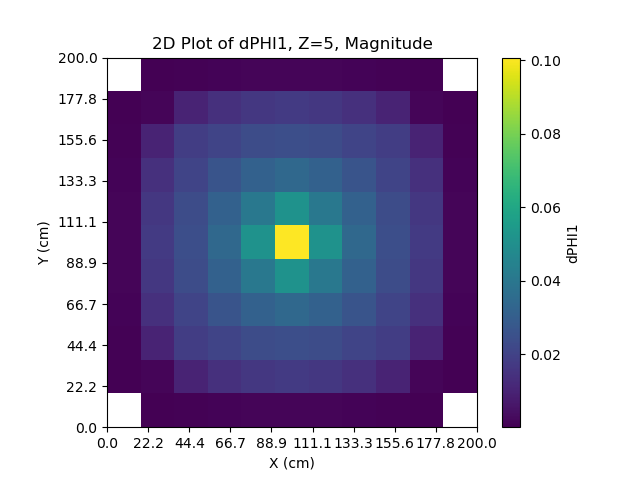
\includegraphics[width=\linewidth]{figures/OBJECTIVES1_TEST10_3DMG_Langenbuch_NOISE_dPHI_magnitude_G1_Z5.png}
        \end{subfigure}
        \hfill
        \begin{subfigure}{.48\textwidth}
          \centering
          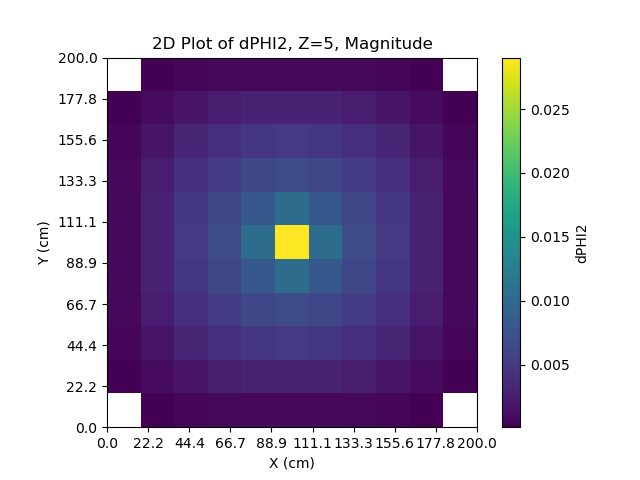
\includegraphics[width=\linewidth]{figures/OBJECTIVES1_TEST10_3DMG_Langenbuch_NOISE_dPHI_magnitude_G2_Z5.png}
        \end{subfigure}
\end{figure}
\begin{figure}[H]\ContinuedFloat
        \centering
        \begin{subfigure}{.48\textwidth}
          \centering
          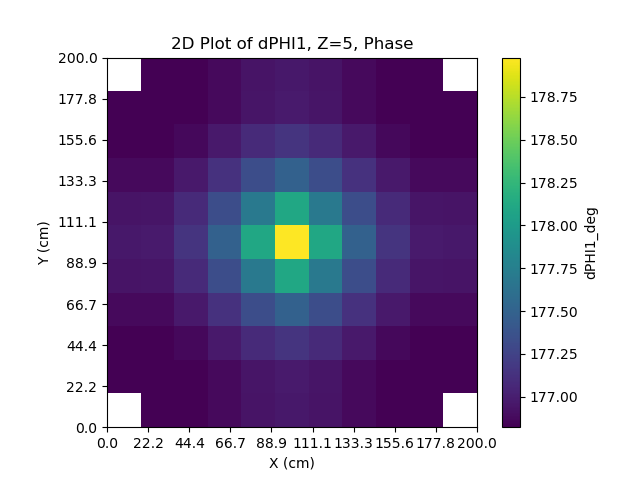
\includegraphics[width=\linewidth]{figures/OBJECTIVES1_TEST10_3DMG_Langenbuch_NOISE_dPHI_phase_G1_Z5.png}
        \end{subfigure}
        \hfill
        \begin{subfigure}{.48\textwidth}
          \centering
          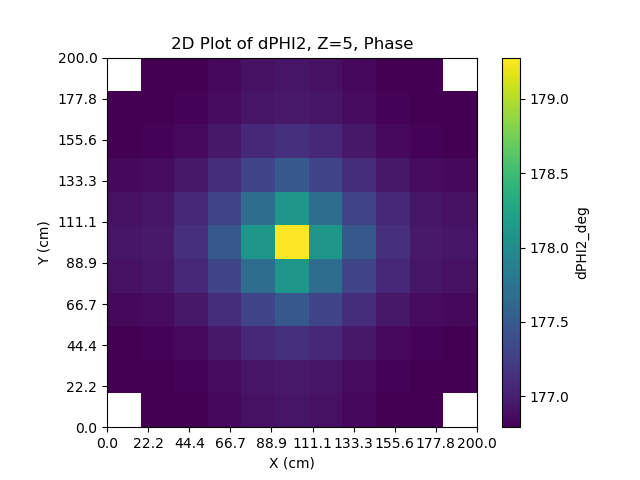
\includegraphics[width=\linewidth]{figures/OBJECTIVES1_TEST10_3DMG_Langenbuch_NOISE_dPHI_phase_G2_Z5.png}
        \end{subfigure}
        \caption{Neutron noise results from the developed solver}
        \label{fig:Langenbuch_noise_results}
\end{figure}

The results show that magnitude of the peak fast neutron noise is larger than the thermal neutron noise. However, the fast neutron noise is more dispersed than the thermal neutron noise. The phase plot shows similarities between fast and thermal group.

\section{3D VVER-400}

\subsection{Forward Simulation}

Water-Water energetic reactor (VVER) is a pressurized water reactor with a possible delivery design of 440 MW among others. This benchmark corresponds to an asymmetric control rod ejection accident in a VVER-440 core. However, only steady-state forward flux simulation is done in this case. The radial and axial configuration of the core is shown in Figure \ref{fig:3DVVER400}, and the homogenized cross-section data is shown in Table \ref{table:3DVVER400XS}. The active core height is 250 cm with 12 planes of assemblies across the core. The data reference of 3D-VVER440 benchmark problem are extracted from \cite{chaoConformalMappingHexagonal1995}.

\begin{figure}[H]
        \centering
        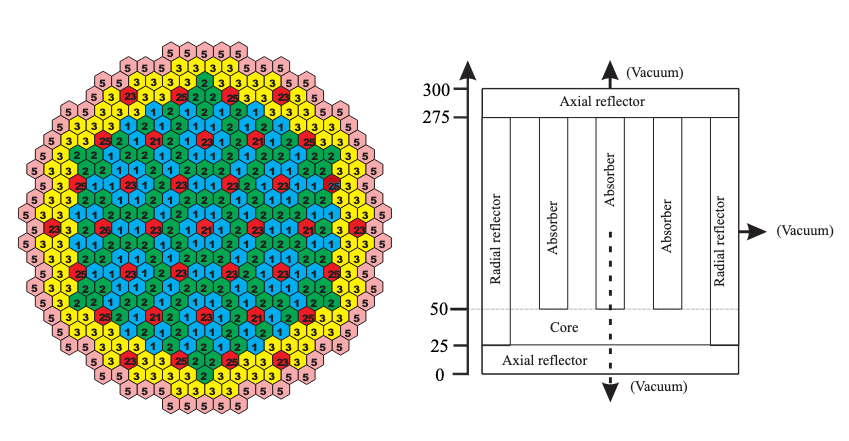
\includegraphics[width=0.7\textwidth]{figures/3DVVER400.png}
        \caption{Core configuration of 3D VVER-400 (obtained from \cite{vidal-ferrandizFEMFFUSIONFiniteElement2023})}
        \label{fig:3DVVER400}
\end{figure}

\begin{table}[H]
        \centering
        \caption{Homogenized cross-section and neutron precursors data of 3D VVER-400 (obtained from \cite{vidal-ferrandizFEMFFUSIONFiniteElement2023})}
        \label{table:3DVVER400XS}
        \begin{tabular}{ | M{4.5cm} | M{1cm} | M{2cm} | M{2cm} | M{2cm} | M{2cm} | } 
         \hline
         \textbf{Material} & \textbf{Group} & \textbf{$D_g$} ($cm$) & \textbf{$\Sigma_{t,g}$} ($cm^{-1}$) & \textbf{$\nu \Sigma_{f,g}$}  ($cm^{-1}$) & \textbf{$\Sigma_{s,1 \rightarrow}$}  ($cm^{-1}$)\\
         \hline
         \multirow{2}{*}{1 - Fuel} & 1 & 1.34660E+00 & 2.52550E-02 & 4.44880E-03 & \\
         \cline{2-6}               & 2 & 3.71690E-01 & 6.42770E-02 & 7.37530E-02 & 1.68930E-02  \\
         \hline
         \multirow{2}{*}{2 - Fuel} & 1 & 1.33770E+00 & 2.47090E-02 & 5.53370E-03 & \\
         \cline{2-6}               & 2 & 3.69180E-01 & 7.93610E-02 & 1.05810E-01 & 1.59120E-02 \\
         \hline
         \multirow{2}{*}{3 - Fuel} & 1 & 1.33220E+00 & 2.43500E-02  & 7.03910E-03 & \\
         \cline{2-6}               & 2 & 3.65020E-01 & 1.00100E-01  & 1.49640E-01 & 1.48880E-02 \\
         \hline
         \multirow{2}{*}{4 - Absorber} & 1 & 1.19530E+00 & 3.56360E-02 & 0.00000E+00 & \\
         \cline{2-6}                   & 2 & 1.93130E-01 & 1.34980E-01 & 0.00000E+00 & 2.22640E-02 \\
         \hline
         \multirow{2}{*}{5 - Radial Reflector} & 1 & 1.44850E+00 & 3.31840E-02 & 0.00000E+00 & \\
         \cline{2-6}                           & 2 & 2.51760E-01 & 3.28390E-02 & 0.00000E+00 & 3.22620E-02 \\
         \hline
         \multirow{2}{*}{6 - Axial Reflector} & 1 & 1.34130E+00 & 2.93010E-02 & 0.00000E+00 & \\
         \cline{2-6}                          & 2 & 2.48710E-01 & 6.46550E-02 & 0.00000E+00 & 2.71480E-02 \\
         \hline
        \end{tabular}
\end{table}

The forward simulation of the 3D VVER-400 has been simulated in FEMFFUSION \cite{vidal-ferrandizFEMFFUSIONFiniteElement2023} and compared with the developed solver. The results are as follows:

\begin{table}[H]
        \centering
        \caption{Eigenvalue results of 3D VVER-400}
        \label{table:3DVVER_fw_results}
        \begin{tabular}{ | M{3.5cm} | M{2cm} | } 
         \hline
         $k_{\text{eff}}$ FEMFFUSION & 1.002440   \\
         \hline
         $k_{\text{eff}}$ solver & 1.003326  \\
         \hline
         Absolute Error (pcm) & 88.6  \\
         \hline
        \end{tabular}
\end{table}

\begin{figure}[H]
        \centering
        \begin{subfigure}{.48\textwidth}
          \centering
          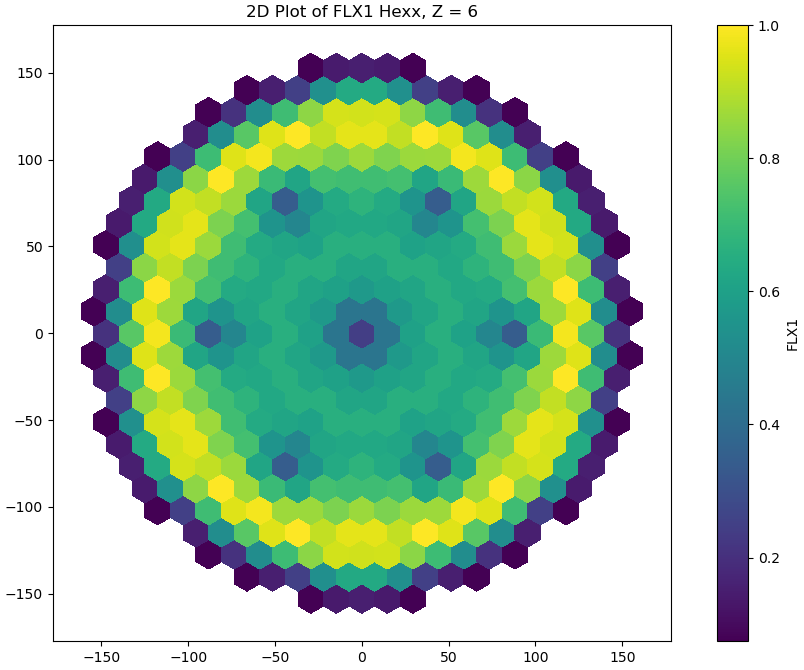
\includegraphics[width=\linewidth]{figures/OBJECTIVES1_TEST07_3DTriMG_VVER400_VandV_level2_FORWARD_FLX_magnitude_G1_Z6.png}
        \end{subfigure}
        \hfill
        \begin{subfigure}{.48\textwidth}
          \centering
          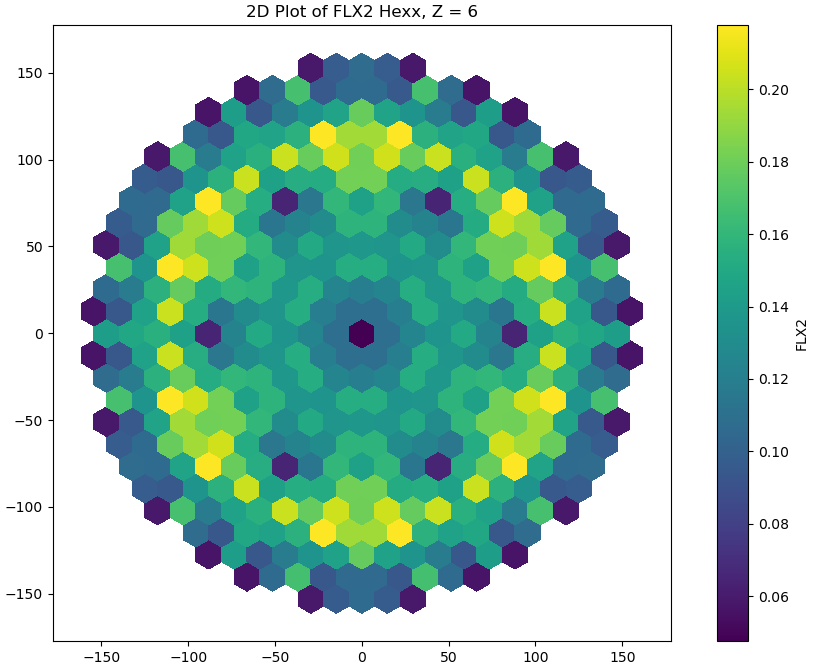
\includegraphics[width=\linewidth]{figures/OBJECTIVES1_TEST07_3DTriMG_VVER400_VandV_level2_FORWARD_FLX_magnitude_G2_Z6.png}
        \end{subfigure}
        \caption{Forward flux results from FEMFFUSION at midplane (Z=6)}
        \label{fig:3DVVER_fw_results_flx}
\end{figure}
\begin{figure}[H]
        \centering
        \begin{subfigure}{.48\textwidth}
          \centering
          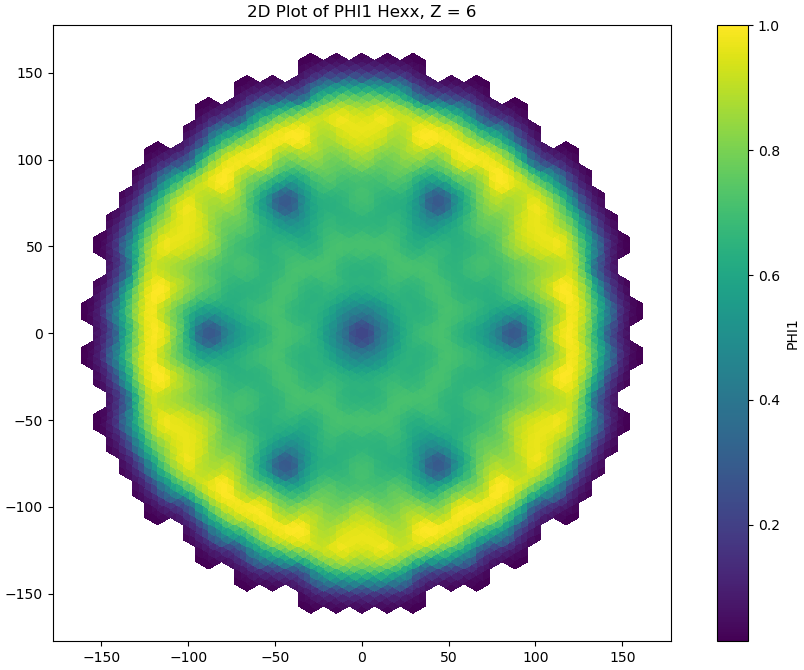
\includegraphics[width=\linewidth]{figures/OBJECTIVES1_TEST07_3DTriMG_VVER400_VandV_level2_FORWARD_PHI_magnitude_G1_Z6.png}
        \end{subfigure}
        \hfill
        \begin{subfigure}{.48\textwidth}
          \centering
          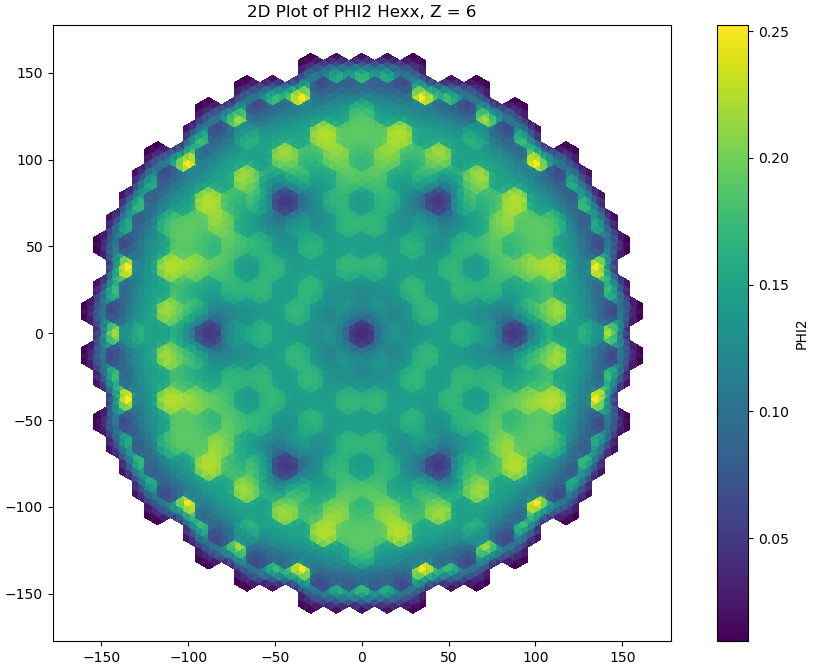
\includegraphics[width=\linewidth]{figures/OBJECTIVES1_TEST07_3DTriMG_VVER400_VandV_level2_FORWARD_PHI_magnitude_G2_Z6.png}
        \end{subfigure}
        \caption{Forward flux results from the developed solver at midplane (Z=6)}
        \label{fig:3DVVER_fw_results_phi}
\end{figure}
\begin{figure}[H]
        \centering
        \begin{subfigure}{.48\textwidth}
          \centering
          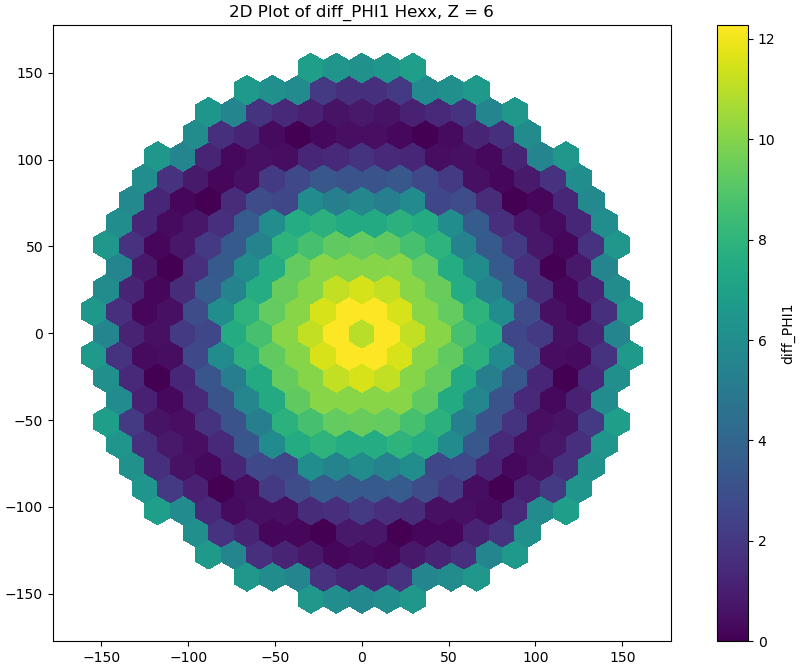
\includegraphics[width=\linewidth]{figures/OBJECTIVES1_TEST07_3DTriMG_VVER400_VandV_level2_FORWARD_diff_PHI_magnitude_G1_Z6.png}
        \end{subfigure}
        \hfill
        \begin{subfigure}{.48\textwidth}
          \centering
          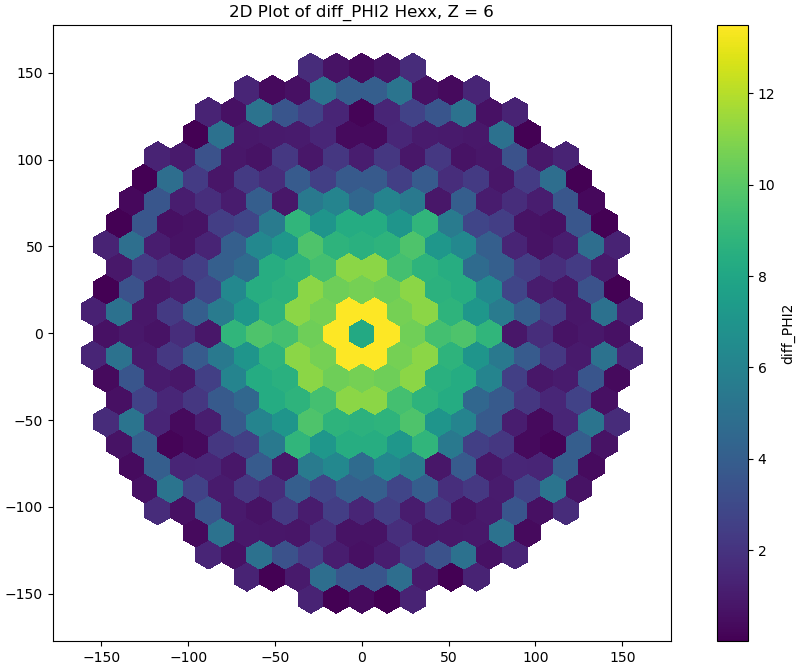
\includegraphics[width=\linewidth]{figures/OBJECTIVES1_TEST07_3DTriMG_VVER400_VandV_level2_FORWARD_diff_PHI_magnitude_G2_Z6.png}
        \end{subfigure}
        \caption{Difference of forward flux between FEMFFUSION and the solver at midplane (Z=6)}
\end{figure}

The forward results show that some discrepancies are observed between the developed solver and FEMFFUSION. The difference in $k_\text{eff}$ is 88.6 pcm and the maximum error of forward flux at midplane is about 12\%. This difference is due to the use of the finite element method in FEMFFUSION, which has different degrees of accuracy compared to the box-scheme finite difference used in the solver. Considering this difference in spatial discretization method, the solver generally works well and in a certain degree of agreement with FEMFFUSION.

\subsection{Neutron Noise Simulation}

For the neutron noise simulation, the noise source is defined as an AVS-type noise source location $\textbf{r}_p$ is near the center of the core and midplane ($Z=7$), indicated by yellow hexagon in Figure \ref{fig:3DVVER_source}. The noise sources are defined as follows:
\begin{equation}
    \begin{aligned}
        \delta \Sigma_{t,2} (\textbf{r}_p, \omega) &= 0.05 \Sigma_{t,2} (\textbf{r}_p)\\    
    \end{aligned}
\end{equation}

\begin{figure}[H]
        \centering
        \begin{subfigure}{.48\textwidth}
          \centering
          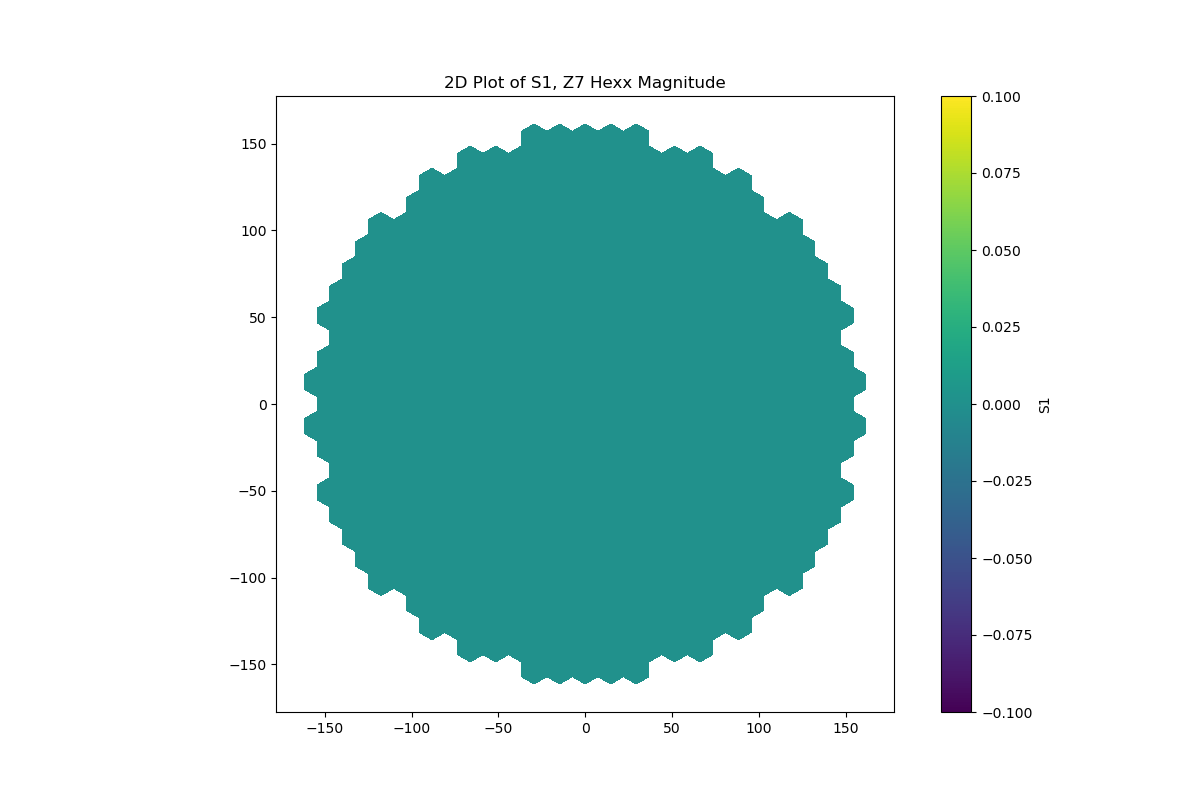
\includegraphics[width=\linewidth]{figures/OBJECTIVES1_TEST07_3DTriMG_VVER400_VandV_level2_NOISE_S_magnitude_G1_Z7.png}
        \end{subfigure}
        \hfill
        \begin{subfigure}{.48\textwidth}
          \centering
          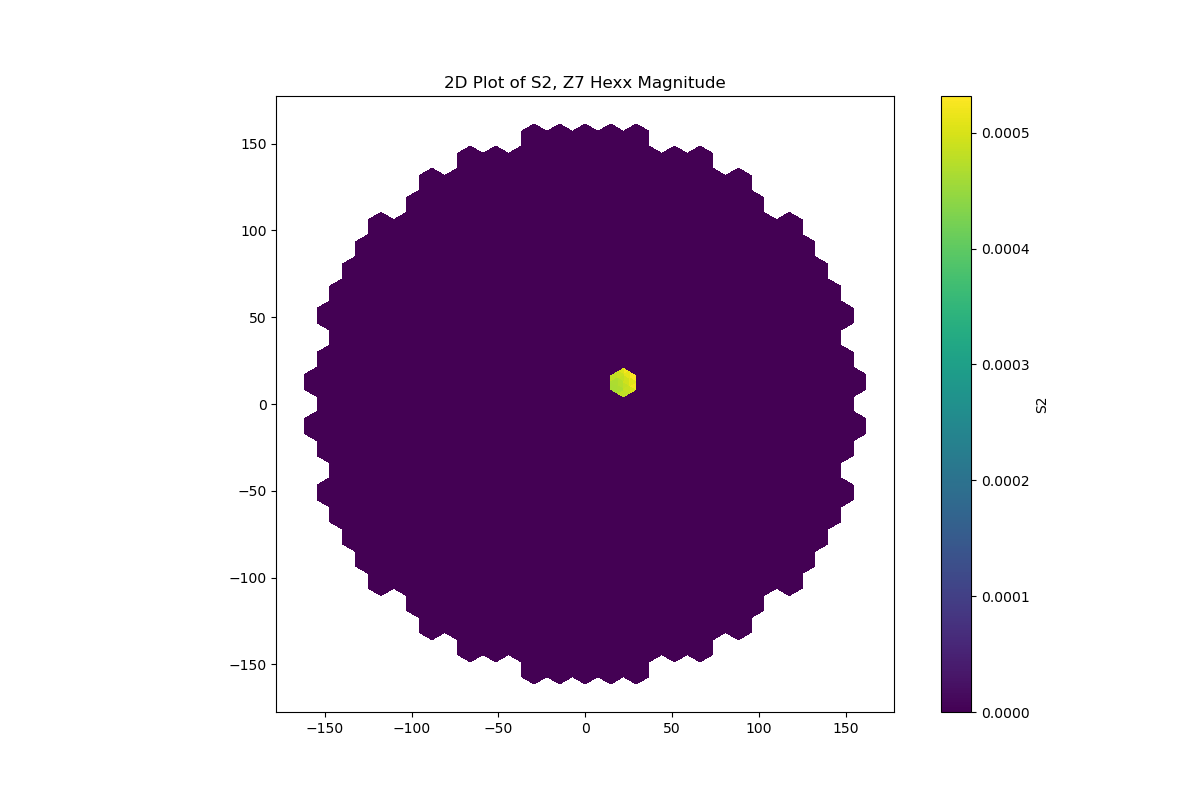
\includegraphics[width=\linewidth]{figures/OBJECTIVES1_TEST07_3DTriMG_VVER400_VandV_level2_NOISE_S_magnitude_G2_Z7.png}
        \end{subfigure}
        \caption{Noise source location for 3D VVER-400}
        \label{fig:3DVVER_source}
\end{figure}

There is no comparison for this simulation. The results of the simulations at the midplane are described in Figure \ref{fig:3DVVER_noise_results}.
\begin{figure}[H]
        \centering
        \begin{subfigure}{.48\textwidth}
          \centering
          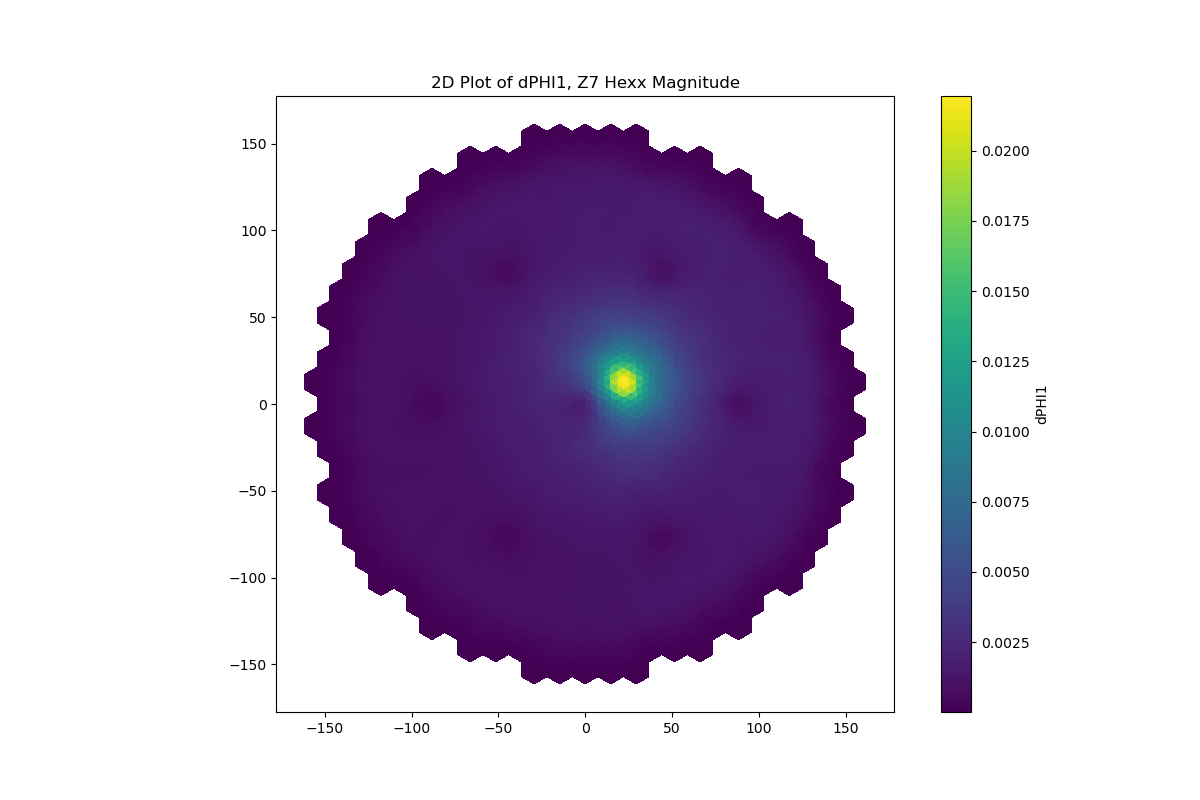
\includegraphics[width=\linewidth]{figures/OBJECTIVES1_TEST07_3DTriMG_VVER400_VandV_level2_NOISE_dPHI_magnitude_G1_Z7.png}
        \end{subfigure}
        \hfill
        \begin{subfigure}{.48\textwidth}
          \centering
          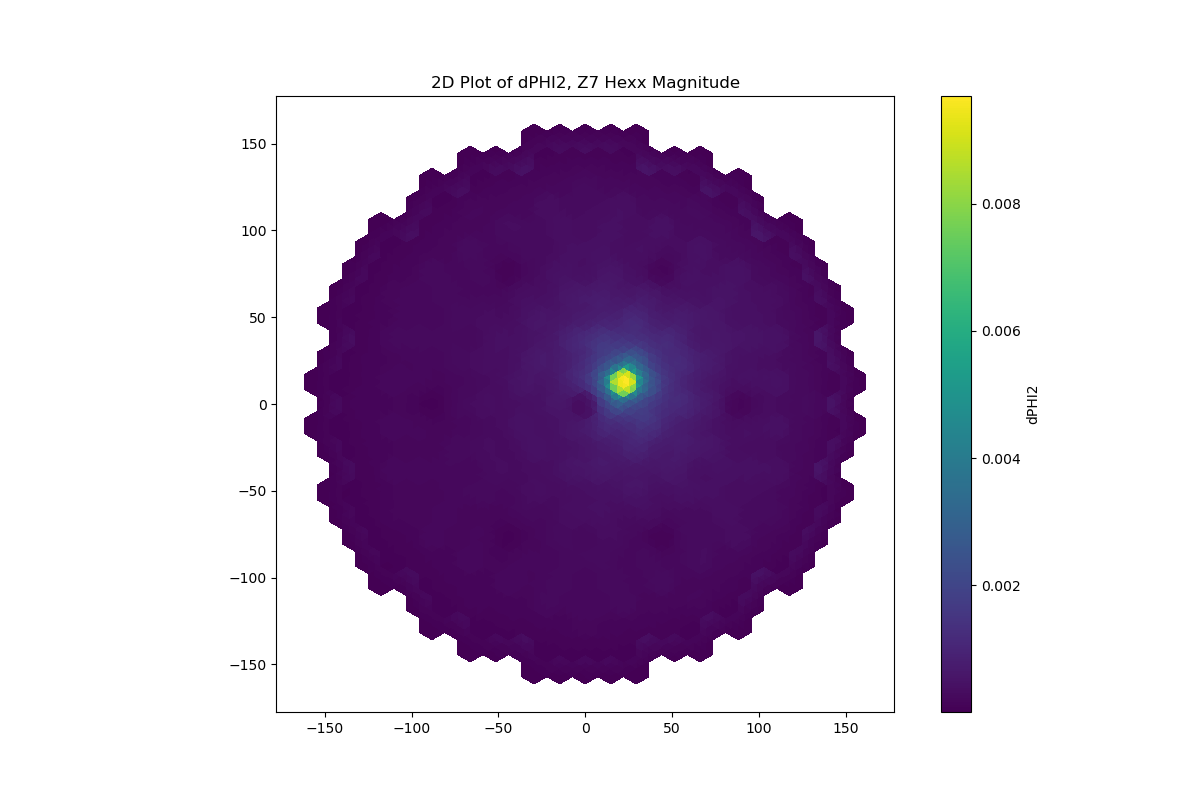
\includegraphics[width=\linewidth]{figures/OBJECTIVES1_TEST07_3DTriMG_VVER400_VandV_level2_NOISE_dPHI_magnitude_G2_Z7.png}
        \end{subfigure}
\end{figure}
\begin{figure}[H]\ContinuedFloat
        \centering
        \begin{subfigure}{.48\textwidth}
          \centering
          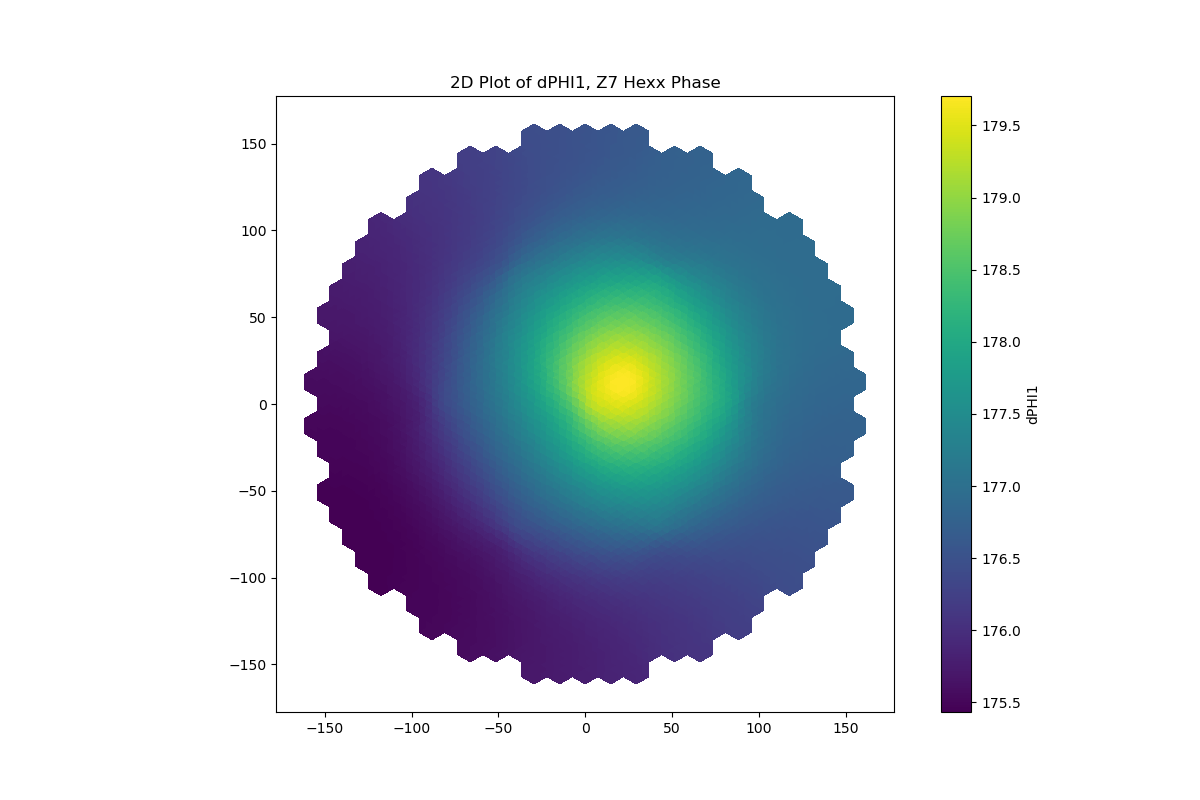
\includegraphics[width=\linewidth]{figures/OBJECTIVES1_TEST07_3DTriMG_VVER400_VandV_level2_NOISE_dPHI_phase_G1_Z7.png}
        \end{subfigure}
        \hfill
        \begin{subfigure}{.48\textwidth}
          \centering
          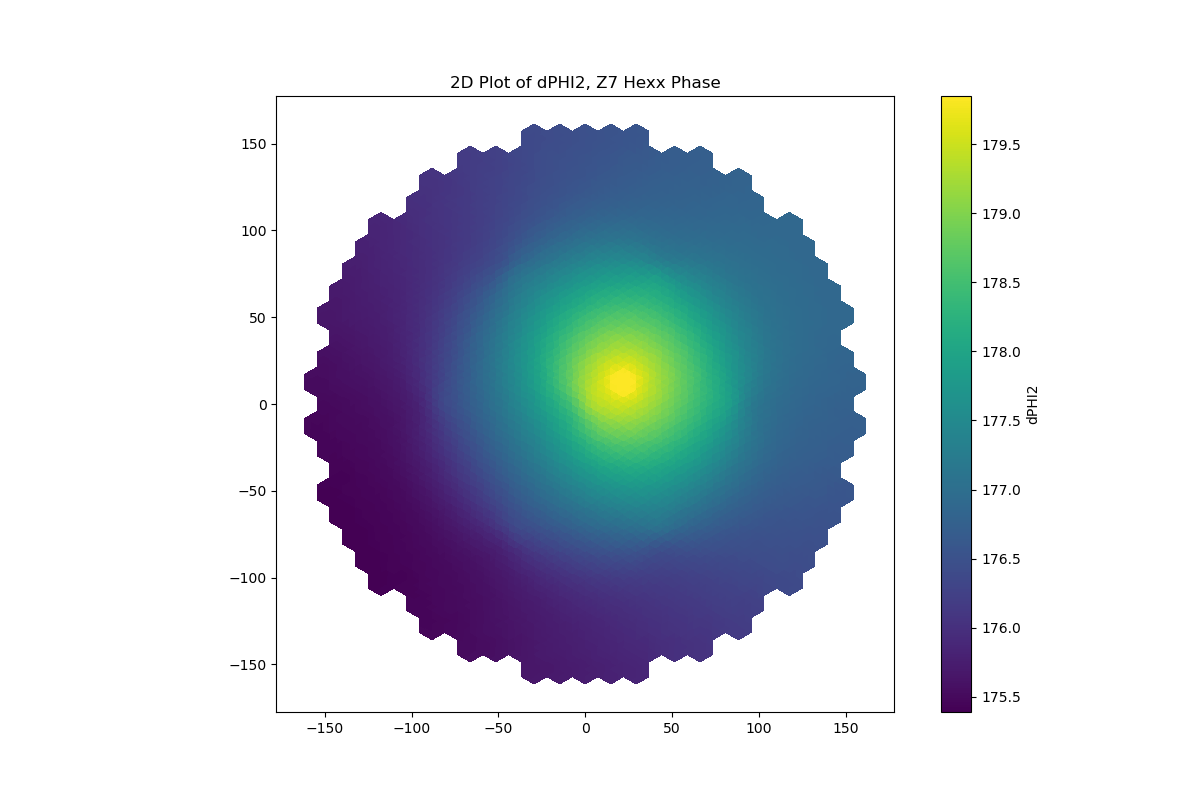
\includegraphics[width=\linewidth]{figures/OBJECTIVES1_TEST07_3DTriMG_VVER400_VandV_level2_NOISE_dPHI_phase_G2_Z7.png}
        \end{subfigure}
        \caption{Neutron noise results from the developed solver}
        \label{fig:3DVVER_noise_results}
\end{figure}

The results show that magnitude of the peak fast neutron noise is larger than the thermal neutron noise. However, the fast neutron noise is more dispersed than the thermal neutron noise. The phase plot shows similarities between fast and thermal group.


\chapter{Backward Elimination Method for Neutron Noise Source Unfolding}
\label{ch:appendixB}

\section{General Overview}

In the backward elimination method, we start with Eq. \ref{eq:greens_function2}, repeated here for convenience.
\begin{equation}\label{eq:greens_function2_back}
    \begin{aligned}
        \delta \phi(\textbf{r}, \omega) &= \sum_{\textbf{r}_p} G(\textbf{r}, \textbf{r}_p,\omega) S(\textbf{r}_p,\omega)
    \end{aligned}
\end{equation}
As seen in Eq. \ref{eq:greens_function2_back}, the neutron noise can be constructed as a finite combination of Green's function matrix and the noise source as the coefficient. This is a finite combination since there are $(\text{group} \times N)^{(\text{group} \times N)}$ possible combinations of solutions that are true in this problem. The backward elimination method starts with the assumption that the noise source is defined in every mesh of the problem. This will overfit the solution of reconstructed neutron noise. Then, for every iteration, the Green's function component that has the smallest contribution to the solution is eliminated. This process is repeated until it finds the smallest possible number of solutions that could pass the residual tolerance. By then, the combination that has the smallest number of components is the solution of the neutron noise vector.

The flow diagram of the method is described in Figure \ref{fig:backward_elimination_method}
\begin{figure}[H]
        \centering
        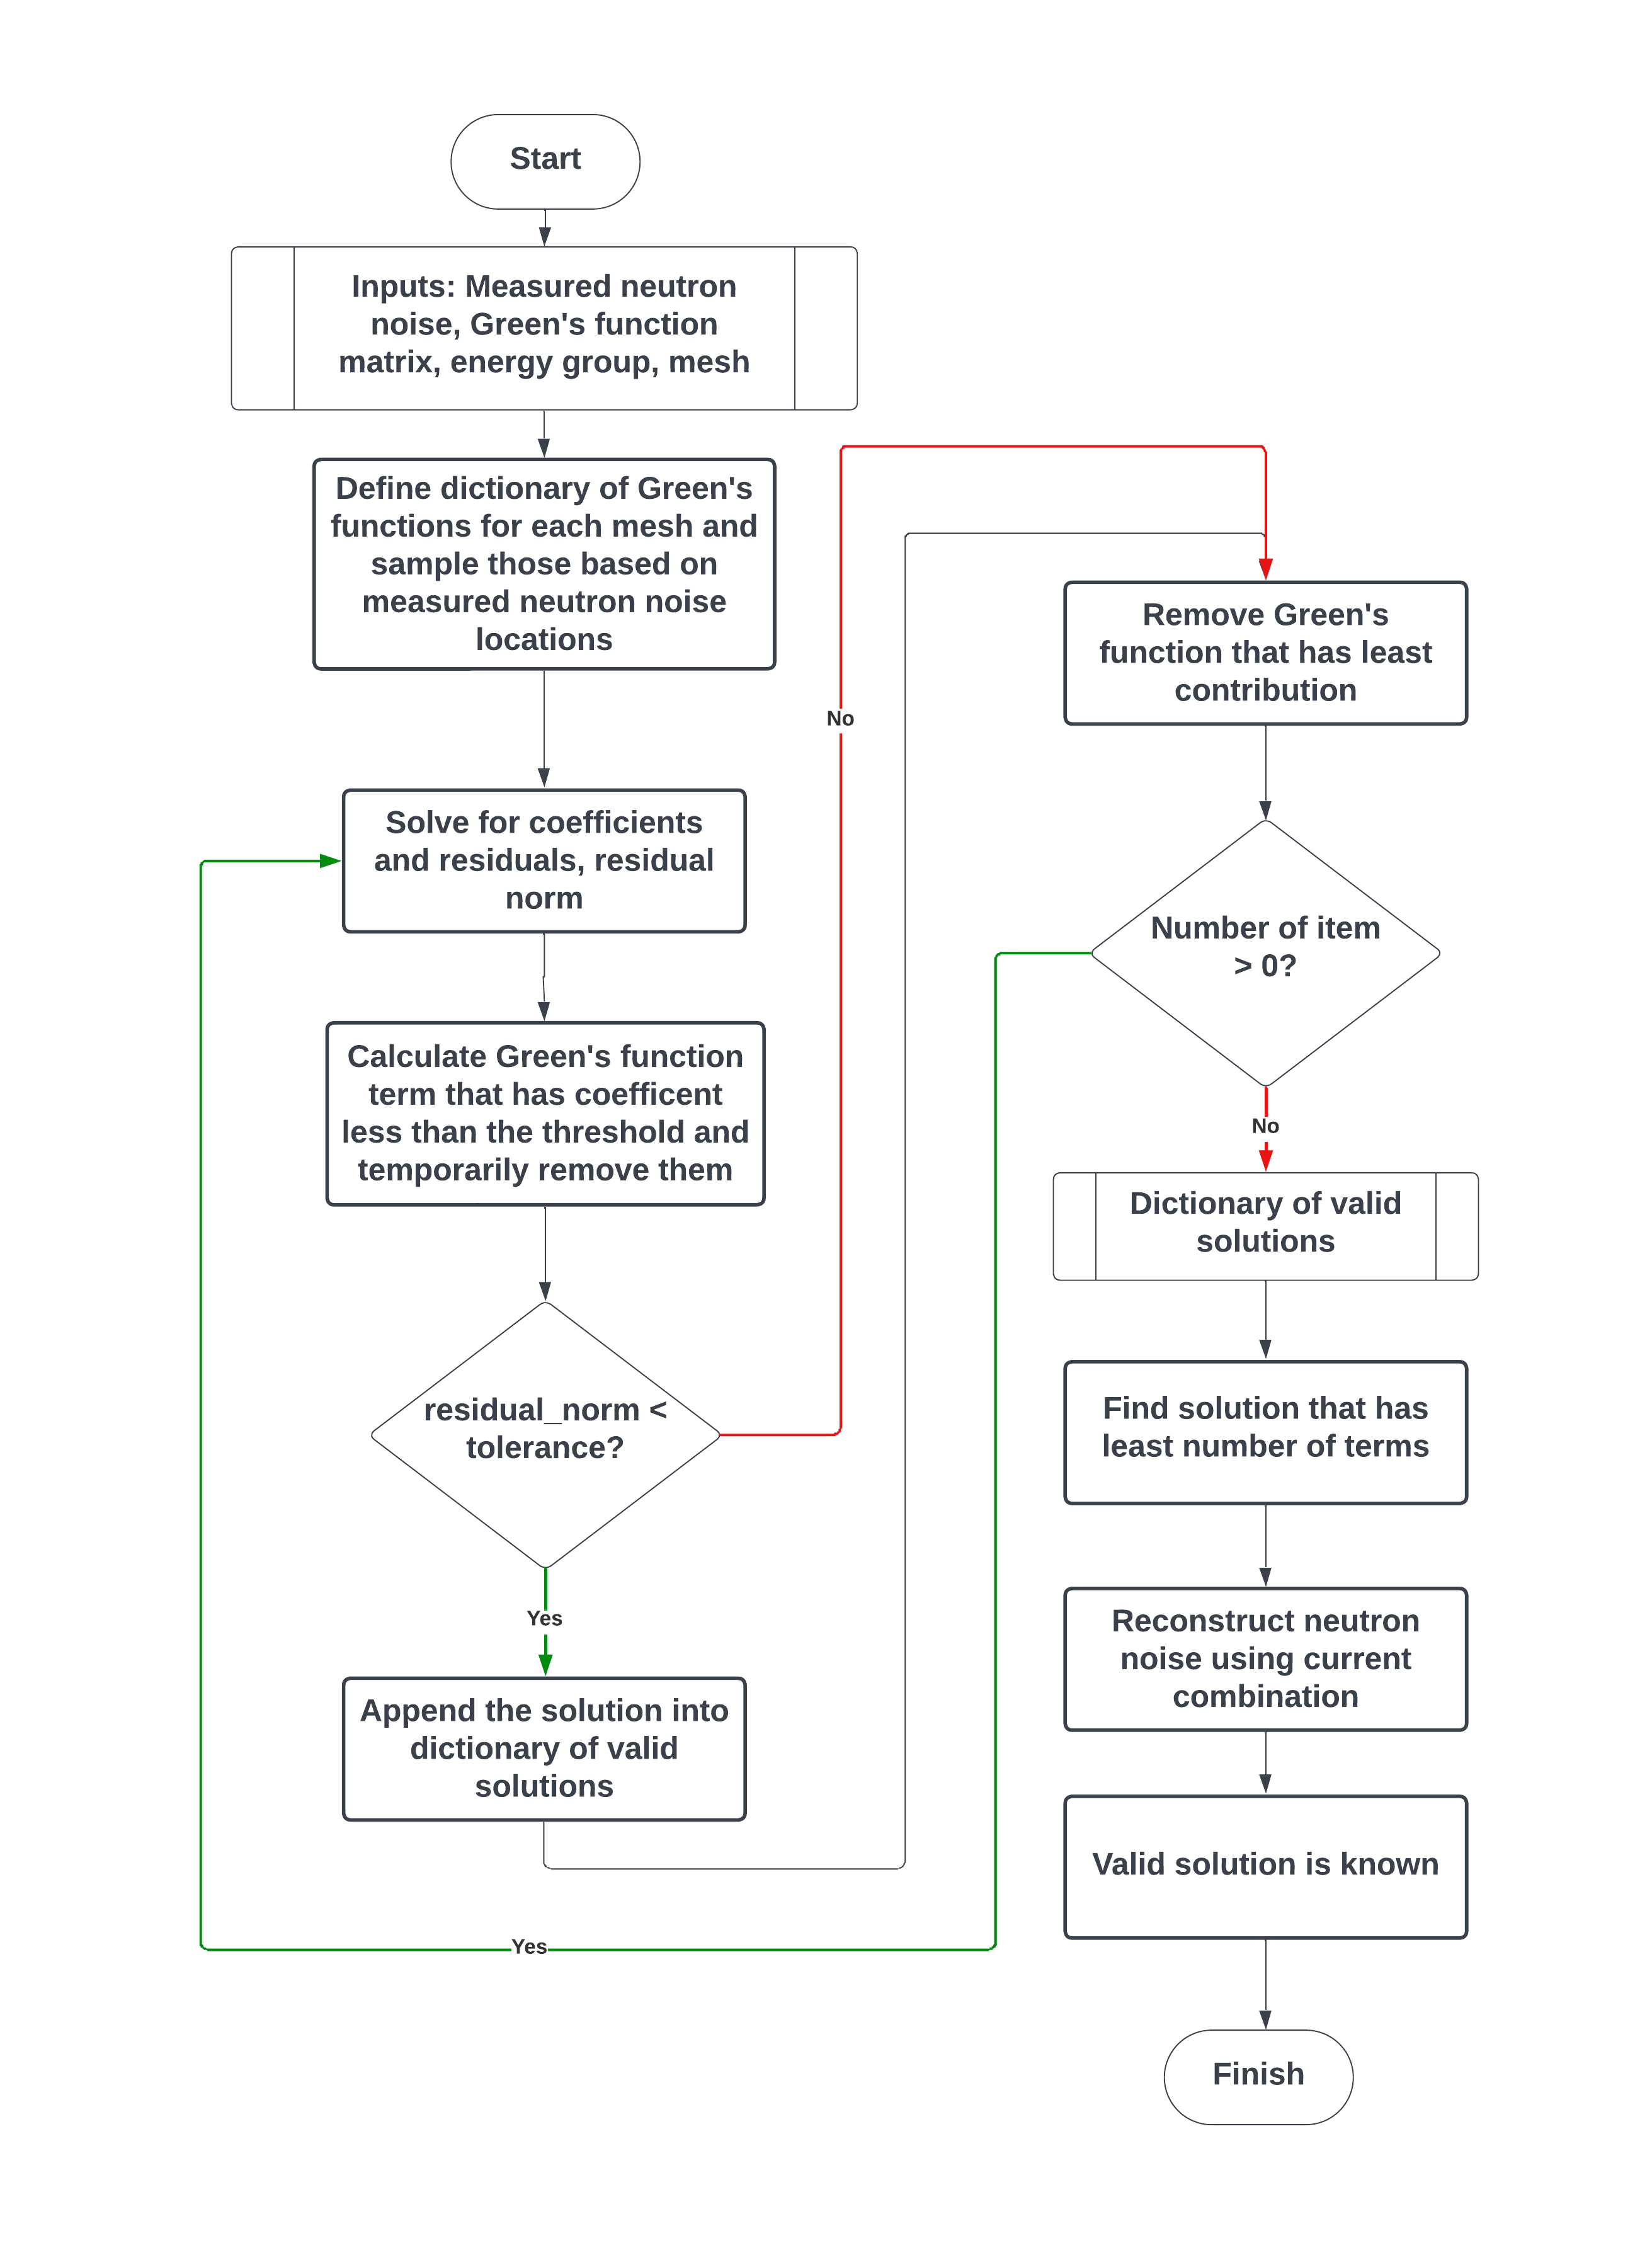
\includegraphics[width=0.6\textwidth]{figures/Backward Elimination.png}
        \caption{Flow diagram of backward elimination method}
        \label{fig:backward_elimination_method}
\end{figure}

The pseudo algorithm for the backward elimination method is described in Algorithm~\ref{alg:backward_unfold}
\begin{algorithm}[H]
\caption{: Backward Elimination Method}
\label{alg:backward_unfold}
\begin{algorithmic}[1]
\Require Measured neutron noise $\delta \phi(\textbf{r}_{\text{meas}}, \omega)$, Green’s function matrix $G(\textbf{r}, \textbf{r}_p,\omega)$, energy groups $g$, mesh $N$
\Ensure Reconstructed neutron noise $\delta \phi_{\text{BACK}}(\textbf{r}, \omega)$, unfolded source $S_{\text{BACK}}(\textbf{r}, \omega)$
\For{each group $g$} \Comment{\textbf{Construct Green’s function dictionary}}
    \For{each node $n$}
        \State Store column $G_{g,n}$ = column of $G(\textbf{r}, \textbf{r}_p,\omega)$ in a dictionary
    \EndFor
\EndFor
\State Sample columns only at measured (non-zero) indices
\State Initialize selected columns $\gets \{ \text{all columns} \}$
\While{selected columns $\neq \emptyset$} \Comment{\textbf{Iterative backward elimination}}
    \State Solve least-squares: $\mathbf{c} = \arg\min ||\delta \phi(\textbf{r}_{\text{meas}}, \omega) - A \mathbf{c}||$ with current columns
    \State Compute residual norm $||r||$
    \State Compute contributions of each column: $|c_i| / \max_j |c_j|$
    \If{$||r|| < \text{tolerance}$}
        \State Store current solution as valid
        \State Remove least contributing column and continue
    \Else
        \State Remove least contributing column
    \EndIf
\EndWhile

\If{no valid solution is found, }  \Comment{\textbf{Select best solution}}
    \State \Return failure
\Else
    \State Select best valid solution (fewest columns)
    \State Reconstruct flux: $\delta \phi_{\text{BACK}}(\textbf{r}, \omega) = \sum c_i G_{i}$
\EndIf
\State Solve $S_{\text{BACK}}(\textbf{r}, \omega) = G^{-1}(\textbf{r}, \textbf{r}_p,\omega) \delta \phi_\text{BACK}(\textbf{r}, \omega)$
\State \textbf{Postprocess:} $S_{\text{BACK}}(\textbf{r}, \omega)$ file, $\delta \phi_\text{BACK}(\textbf{r}, \omega)$ file, plots. 
\end{algorithmic}
\end{algorithm}

This method is applied to 2D HTTR problems similar to the problems in Section \ref{ch:unfolding_methods}. The results are described in the following section.

\section{Application of HTTR Core}

\subsection{2D HTTR with Absorber of Variable Strength Source}

\subsubsection{Single Noise Source}

In this simulation, single mesh AVS source is unfolded using both the existing and novel methods. The simulation is done with a constant frequency of 0.316 Hz. Figure \ref{fig:map_S_2DHTTR_AVS1S_back} shows the location of the AVS source.
\begin{figure}[H]
        \centering
        \begin{subfigure}{.48\textwidth}
          \centering
          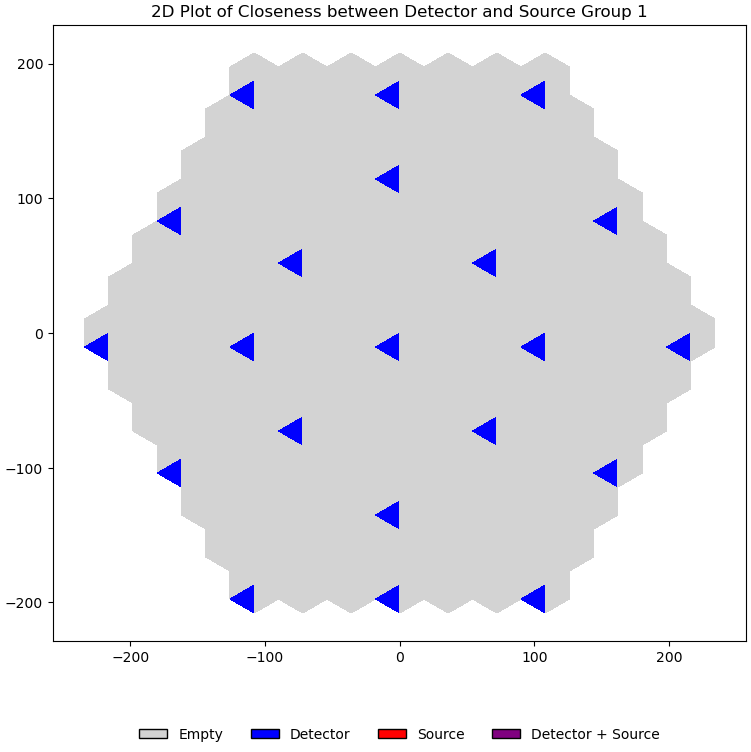
\includegraphics[width=\linewidth]{figures/OBJECTIVES61_TEST_SUITE_2DTriMG_HTTR_level1_iter2_closeness_det_S_categorical_G1.png}
        \end{subfigure}
        \hfill
        \begin{subfigure}{.48\textwidth}
          \centering
          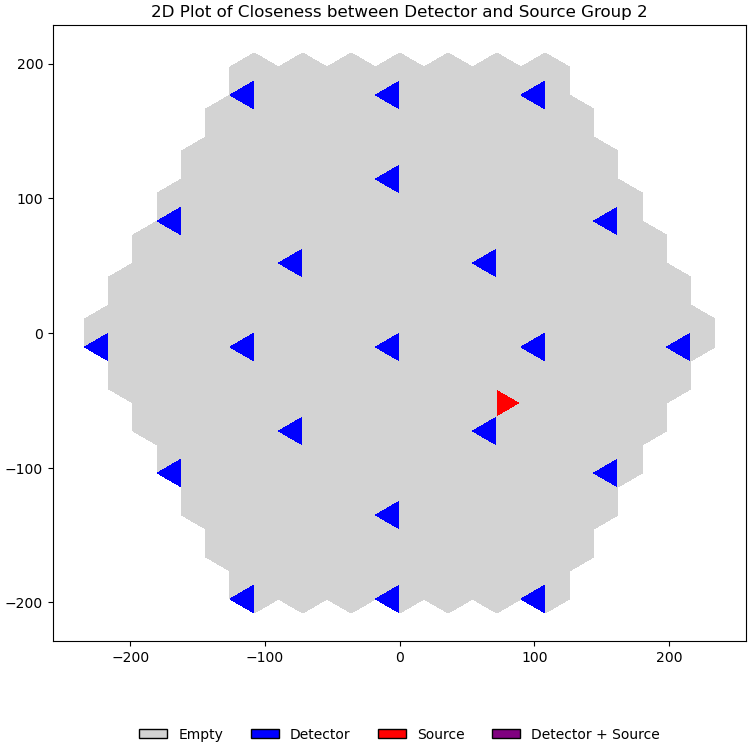
\includegraphics[width=\linewidth]{figures/OBJECTIVES61_TEST_SUITE_2DTriMG_HTTR_level1_iter2_closeness_det_S_categorical_G2.png}
        \end{subfigure}
        \caption{Location of source and detectors in the 2D HTTR case}
        \label{fig:map_S_2DHTTR_AVS1S_back}
\end{figure}

The results of the simulations are described in Table \ref{table:unfold_2DHTTR_AVS1S_back}.
\begin{table}[H]
        \centering
        \caption{Single noise source in 2D HTTR}
        \label{table:unfold_2DHTTR_AVS1S_back}
        \begin{tabular}{ | M{3.5cm} | M{1.5cm} | M{1.5cm} | M{4cm} | M{1.5cm} | } 
         \hline
         \textbf{Method} & \textbf{Energy Group} & \textbf{Hex Number} & \textbf{Neutron Noise Source} ($n/cm^3$) & \textbf{Match?}  \\
         \hline
         Reference & 2 & 42 & $-3.094 \times 10^{-4} + 0.000i$ & --  \\
         \hline
         Backward Elimination & 2 & 42 & $-3.094 \times 10^{-4} + 0.000i$ & Yes  \\
         \hline
        \end{tabular}
\end{table}
The results indicate that the backward elimination method is effective for a single mesh source. This is because the method iterates to find the least number of Green's function combinations that can match the reference.

\subsubsection{Multiple Noise Source}

In this simulation, two-mesh and three-mesh AVS source is unfolded using both the existing and novel methods. For the two-mesh source, the simulation is done with a constant frequency of 10 Hz. Figure \ref{fig:map_S_2DHTTR_AVS2S_back} shows the location of the AVS source.
\begin{figure}[H]
        \centering
        \begin{subfigure}{.48\textwidth}
          \centering
          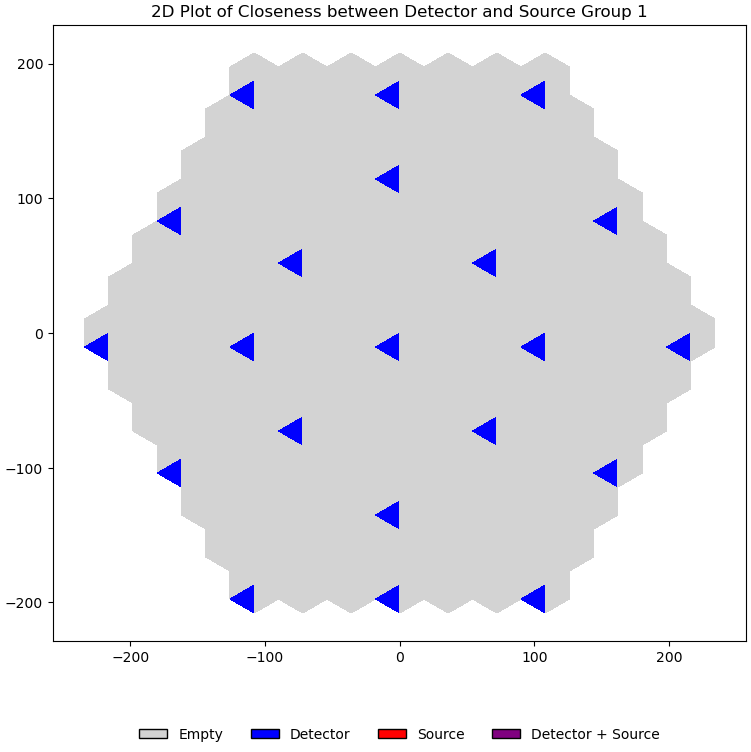
\includegraphics[width=\linewidth]{figures/OBJECTIVES61_TEST_SUITE_2DTriMG_HTTR_level1_iter9_closeness_det_S_categorical_G1.png}
        \end{subfigure}
        \hfill
        \begin{subfigure}{.48\textwidth}
          \centering
          \includegraphics[width=\linewidth]{figures/OBJECTIVES61_TEST_SUITE_2DTriMG_HTTR_level1_iter9_closeness_det_S_categorical_G2.png}
        \end{subfigure}
        \caption{Location of sources and detectors in the 2D HTTR case}
        \label{fig:map_S_2DHTTR_AVS2S_back}
\end{figure}

The results of the simulations are described in Table \ref{table:unfold_2DHTTR_AVS2S_back}.
\begin{table}[H]
        \centering
        \caption{Two noise sources in 2D HTTR}
        \label{table:unfold_2DHTTR_AVS2S_back}
        \begin{tabular}{ | M{3.5cm} | M{1.5cm} | M{1.5cm} | M{4.5cm} | M{1.5cm} | } 
         \hline
         \textbf{Method} & \textbf{Energy Group} & \textbf{Hex Number} & \textbf{Neutron Noise Source} ($n/cm^3$) & \textbf{Match?}  \\
         \hline
         \multirow{2}{*}{Reference} & 2 & 98 & $-1.054 \times 10^{-2}-9.373 \times 10^{-3}j$ & 1  \\
         \cline{2-5}                & 2 & 112 & $-1.739 \times 10^{-4}+0.000i$ & --  \\
         \hline
         \multirow{2}{*}{Backward Elimination} & 2 & 96 & $2.631 \times 10^{-2} - 2.443 \times 10^{-3}i$ & No  \\
         \cline{2-5}                           & 2 & 120 & $-2.598 \times 10^{-2} - 6.998 \times 10^{-5}i$ & No  \\
         \hline
        \end{tabular}
\end{table}

For the three-mesh source, the simulation is done with a constant frequency of 1 Hz. Figure \ref{fig:map_S_2DHTTR_AVS3S_back} shows the location of the AVS source.
\begin{figure}[H]
        \centering
        \begin{subfigure}{.48\textwidth}
          \centering
          \includegraphics[width=\linewidth]{figures/OBJECTIVES45_TEST10_2DTriMG_HTTR_AVS3S_level1_closeness_det_S_categorical_G1.png}
        \end{subfigure}
        \hfill
        \begin{subfigure}{.48\textwidth}
          \centering
          \includegraphics[width=\linewidth]{figures/OBJECTIVES45_TEST10_2DTriMG_HTTR_AVS3S_level1_closeness_det_S_categorical_G2.png}
        \end{subfigure}
        \caption{Location of sources and detectors in the 2D HTTR case}
        \label{fig:map_S_2DHTTR_AVS3S_back}
\end{figure}

The results of the simulations are described in Table \ref{table:unfold_2DHTTR_AVS3S_back}.
\begin{table}[H]
        \centering
        \caption{Three noise sources in 2D HTTR}
        \label{table:unfold_2DHTTR_AVS3S_back}
        \begin{tabular}{ | M{3.5cm} | M{1.5cm} | M{1.5cm} | M{4.5cm} | M{1.5cm} | } 
         \hline
         \textbf{Method} & \textbf{Energy Group} & \textbf{Hex Number} & \textbf{Neutron Noise Source} ($n/cm^3$) & \textbf{Match?}  \\
         \hline
         \multirow{3}{*}{Reference} & 1 & 18 & $-2.797 \times 10^{-8} + 0.000i$ & --  \\
         \cline{2-5}                & 2 & 32 & $-3.341 \times 10^{-6} + 0.000i$ & --  \\
         \cline{2-5}                & 2 & 38 & $-1.053 \times 10^{-4} + 0.000i$ & --  \\
         \hline
         \multirow{3}{*}{Backward Elimination} & 1 & 4 & $-1.178 \times 10^{-1} + 8.899 \times 10^{-4}i$ & No  \\
         \cline{2-5}                           & 2 & 4 & $7.709 \times 10^{-2} - 7.359 \times 10^{-4}i$ & No  \\
         \cline{2-5}                           & 1 & 13 & $6.236 \times 10^{-2} - 4.682 \times 10^{-4}i$ & No  \\
         \hline
        \end{tabular}
\end{table}

The results indicate that the backward elimination method is ineffective in simultaneously unfolding multiple neutron noise sources. This is because during the iteration, it is possible that the Green's functions of the position of the neutron noise source are eliminated. The elimination can happen if, at that combination, the Green's functions that are supposed to be the solution of the problem have small contributions to the solution. This makes the backward elimination method unreliable for unfolding multiple neutron noise sources simultaneously.

\chapter{Combinations for Greedy Method Scoping}
\label{ch:appendixC}

For the purpose of scoping to test the limits of greedy method in Section \ref{sec:greedy_limit}, the ranges of different variables are defined as follows:
\begin{itemize}
    \item \textbf{Frequency}: 10 values evenly spaced in logarithmic scale between 0.01 Hz to 10 Hz. 
    \item \textbf{Magnitude}: For both real numbers and imaginary number, random between 1\% to 10\% of nominal cross-section. It is also randomly choose to add imaginary number or not.
    \item \textbf{Energy group}: Random between 1 (fast) and 2 (thermal).
    \item \textbf{Location}: Random at any mesh (in this case, 1 to 762).
\end{itemize}

For the simulation with 21 detectors, the variable values are tabulated in Table \ref{table:greedy_values_21}.

\begin{longtable}{ | M{2.0cm} | M{2.0cm} | M{1.5cm} | M{1.5cm} | M{2.0cm} | M{2.0cm} | M{1.5cm} | }
\caption{Variable Values in Greedy Method for 21 detectors} \label{table:greedy_values_21}\\
\hline
\textbf{Number of Sources} & \textbf{Frequency} (Hz) & \textbf{Energy Group} & \textbf{Mesh Number} & \textbf{Real Magnitude} & \textbf{Imag. Magnitude} & \textbf{Match?} \\
\hline
\endfirsthead

\caption[]{Variable Values in Greedy Method for 21 detectors (cont.)} \\   % Note the empty [] to avoid duplicate list-of-tables entry
\hline
\textbf{Number of Sources} & \textbf{Frequency} (Hz) & \textbf{Energy Group} & \textbf{Mesh Number} & \textbf{Real Magnitude} & \textbf{Imag. Magnitude} & \textbf{Match?} \\
\hline
\endhead

\hline
\multicolumn{7}{r}{\small Variable Values in Greedy Method for 21 detectors (cont.)} \\
\endfoot

\hline
\endlastfoot
         \multirow{2}{*}{1} & 0.01 & 1 & 22  & 0.04 & 0.02 & Yes \\
         \cline{2-7}        & 0.02 & 2 & 13  & 0.09 & 0.00 & Yes \\
         \cline{2-7}        & 0.05 & 1 & 210 & 0.08 & 0.09 & Yes \\
         \cline{2-7}        & 0.10 & 2 & 47  & 0.04 & 0.00 & Yes \\
         \cline{2-7}        & 0.20 & 2 & 400 & 0.02 & 0.00 & Yes \\
         \cline{2-7}        & 0.50 & 2 & 534 & 0.09 & 0.01 & Yes \\
         \cline{2-7}        & 1.00 & 2 & 475 & 0.04 & 0.00 & Yes \\
         \cline{2-7}        & 2.15 & 1 & 658 & 0.1  & 0.06 & Yes \\
         \cline{2-7}        & 4.64 & 1 & 606 & 0.09 & 0.07 & Yes \\
         \cline{2-7}        & 10.0 & 2 & 23  & 0.1  & 0.06 & Yes \\
         \hline
         \multirow{2}{*}{2} & 0.01 & 2 & 400 & 0.03 & 0.08 & Yes \\
         \cline{2-7}        & 0.01 & 2 & 348 & 0.07 & 0.02 & Yes \\
         \cline{2-7}        & 0.02 & 1 & 446 & 0.03 & 0.08 & Yes \\
         \cline{2-7}        & 0.02 & 1 & 247 & 0.07 & 0.00 & Yes \\
         \cline{2-7}        & 0.05 & 2 & 741 & 0.05 & 0.00 & Yes \\
         \cline{2-7}        & 0.05 & 2 & 423 & 0.05 & 0.01 & Yes \\
         \cline{2-7}        & 0.10 & 2 & 573 & 0.07 & 0.00 & Yes \\
         \cline{2-7}        & 0.10 & 2 & 103 & 0.05 & 0.06 & Yes \\
         \cline{2-7}        & 0.20 & 2 & 710 & 0.07 & 0.02 & Yes \\
         \cline{2-7}        & 0.20 & 1 & 463 & 0.01 & 0.03 & Yes \\
         \cline{2-7}        & 0.50 & 2 & 758 & 0.04 & 0.09 & Yes \\
         \cline{2-7}        & 0.50 & 2 & 214 & 0.01 & 0.00 & Yes \\
         \cline{2-7}        & 1.00 & 1 & 91  & 0.09 & 0.04 & Yes \\
         \cline{2-7}        & 1.00 & 2 & 363 & 0.09 & 0.02 & Yes \\
         \cline{2-7}        & 2.15 & 1 & 446 & 0.04 & 0.03 & Yes \\
         \cline{2-7}        & 2.15 & 1 & 719 & 0.03 & 0.00 & Yes \\
         \cline{2-7}        & 4.64 & 1 & 31  & 0.05 & 0.00 & Yes \\
         \cline{2-7}        & 4.64 & 2 & 419 & 0.09 & 0.08 & Yes \\
         \cline{2-7}        & 10.0 & 2 & 469 & 0.01 & 0.01 & Yes \\
         \cline{2-7}        & 10.0 & 2 & 74  & 0.01 & 0.07 & Yes \\
         \hline
         \multirow{2}{*}{3} & 0.01 & 1 & 667 & 0.08 & 0.00 & Yes \\
         \cline{2-7}        & 0.01 & 1 & 543 & 0.07 & 0.07 & Yes \\
         \cline{2-7}        & 0.01 & 2 & 721 & 0.09 & 0.00 & Yes \\
         \cline{2-7}        & 0.02 & 2 & 674 & 0.04 & 0.00 & Yes \\
         \cline{2-7}        & 0.02 & 2 & 6   & 0.07 & 0.00 & Yes \\
         \cline{2-7}        & 0.02 & 1 & 611 & 0.06 & 0.00 & Yes \\
         \cline{2-7}        & 0.05 & 2 & 742 & 0.06 & 0.00 & Yes \\
         \cline{2-7}        & 0.05 & 1 & 667 & 0.01 & 0.01 & Yes \\
         \cline{2-7}        & 0.05 & 2 & 530 & 0.09 & 0.00 & Yes \\
         \cline{2-7}        & 0.10 & 2 & 724 & 0.10 & 0.00 & Yes \\
         \cline{2-7}        & 0.10 & 2 & 354 & 0.10 & 0.00 & Yes \\
         \cline{2-7}        & 0.10 & 1 & 385 & 0.10 & 0.01 & Yes \\
         \cline{2-7}        & 0.20 & 1 & 66  & 0.02 & 0.00 & Yes \\
         \cline{2-7}        & 0.20 & 2 & 75  & 0.02 & 0.04 & Yes \\
         \cline{2-7}        & 0.20 & 2 & 759 & 0.05 & 0.00 & Yes \\
         \cline{2-7}        & 0.50 & 2 & 186 & 0.09 & 0.00 & Yes \\
         \cline{2-7}        & 0.50 & 2 & 362 & 0.03 & 0.07 & Yes \\
         \cline{2-7}        & 0.50 & 1 & 534 & 0.07 & 0.05 & Yes \\
         \cline{2-7}        & 1.00 & 2 & 491 & 0.09 & 0.00 & Yes \\
         \cline{2-7}        & 1.00 & 2 & 693 & 0.04 & 0.04 & Yes \\
         \cline{2-7}        & 1.00 & 2 & 5   & 0.09 & 0.06 & Yes \\
         \cline{2-7}        & 2.15 & 2 & 156 & 0.08 & 0.00 & Yes \\
         \cline{2-7}        & 2.15 & 1 & 629 & 0.03 & 0.01 & Yes \\
         \cline{2-7}        & 2.15 & 2 & 66  & 0.06 & 0.00 & Yes \\
         \cline{2-7}        & 4.64 & 2 & 42  & 0.02 & 0.00 & Yes \\
         \cline{2-7}        & 4.64 & 1 & 110 & 0.02 & 0.03 & Yes \\
         \cline{2-7}        & 4.64 & 2 & 750 & 0.10 & 0.03 & Yes \\
         \cline{2-7}        & 10.0 & 1 & 73  & 0.01 & 0.00 & Yes \\
         \cline{2-7}        & 10.0 & 2 & 386 & 0.03 & 0.00 & Yes \\
         \cline{2-7}        & 10.0 & 2 & 120 & 0.04 & 0.07 & Yes \\
         \hline
         \multirow{2}{*}{4} & 0.01 & 2 & 656 & 0.03 & 0.00 & Yes \\
         \cline{2-7}        & 0.01 & 1 & 435 & 0.01 & 0.00 & Yes \\
         \cline{2-7}        & 0.01 & 1 & 300 & 0.09 & 0.00 & Yes \\
         \cline{2-7}        & 0.01 & 1 & 305 & 0.03 & 0.02 & Yes \\
         \cline{2-7}        & 0.02 & 1 & 640 & 0.08 & 0.08 & Yes \\
         \cline{2-7}        & 0.02 & 2 & 753 & 0.01 & 0.10 & Yes \\
         \cline{2-7}        & 0.02 & 1 & 147 & 0.10 & 0.03 & Yes \\
         \cline{2-7}        & 0.02 & 1 & 249 & 0.04 & 0.02 & Yes \\
         \cline{2-7}        & 0.05 & 2 & 402 & 0.01 & 0.04 & Yes \\
         \cline{2-7}        & 0.05 & 1 & 111 & 0.06 & 0.00 & Yes \\
         \cline{2-7}        & 0.05 & 1 & 613 & 0.04 & 0.01 & Yes \\
         \cline{2-7}        & 0.05 & 1 & 393 & 0.06 & 0.05 & Yes \\
         \cline{2-7}        & 0.10 & 2 & 606 & 0.08 & 0.00 & Yes \\
         \cline{2-7}        & 0.10 & 2 & 109 & 0.07 & 0.06 & Yes \\
         \cline{2-7}        & 0.10 & 2 & 106 & 0.01 & 0.05 & Yes \\
         \cline{2-7}        & 0.10 & 1 & 304 & 0.01 & 0.06 & Yes \\
         \cline{2-7}        & 0.20 & 2 & 327 & 0.10 & 0.09 & Yes \\
         \cline{2-7}        & 0.20 & 2 & 562 & 0.02 & 0.01 & Yes \\
         \cline{2-7}        & 0.20 & 2 & 266 & 0.07 & 0.06 & Yes \\
         \cline{2-7}        & 0.20 & 2 & 487 & 0.05 & 0.01 & Yes \\
         \cline{2-7}        & 0.50 & 1 & 419 & 0.09 & 0.08 & Yes \\
         \cline{2-7}        & 0.50 & 2 & 728 & 0.10 & 0.10 & Yes \\
         \cline{2-7}        & 0.50 & 1 & 504 & 0.07 & 0.10 & Yes \\
         \cline{2-7}        & 0.50 & 2 & 83  & 0.10 & 0.05 & Yes \\
         \cline{2-7}        & 1.00 & 1 & 704 & 0.07 & 0.00 & Yes \\
         \cline{2-7}        & 1.00 & 1 & 16  & 0.05 & 0.00 & Yes \\
         \cline{2-7}        & 1.00 & 2 & 186 & 0.04 & 0.00 & Yes \\
         \cline{2-7}        & 1.00 & 2 & 640 & 0.10 & 0.00 & Yes \\
         \cline{2-7}        & 2.15 & 1 & 1   & 0.05 & 0.03 & Yes \\
         \cline{2-7}        & 2.15 & 2 & 90  & 0.09 & 0.00 & Yes \\
         \cline{2-7}        & 2.15 & 1 & 414 & 0.10 & 0.10 & Yes \\
         \cline{2-7}        & 2.15 & 2 & 320 & 0.05 & 0.00 & Yes \\
         \cline{2-7}        & 4.64 & 1 & 217 & 0.07 & 0.00 & Yes \\
         \cline{2-7}        & 4.64 & 2 & 484 & 0.03 & 0.10 & Yes \\
         \cline{2-7}        & 4.64 & 1 & 531 & 0.01 & 0.00 & Yes \\
         \cline{2-7}        & 4.64 & 1 & 641 & 0.05 & 0.00 & Yes \\
         \cline{2-7}        & 10.0 & 2 & 237 & 0.06 & 0.07 & Yes \\
         \cline{2-7}        & 10.0 & 1 & 666 & 0.04 & 0.08 & Yes \\
         \cline{2-7}        & 10.0 & 1 & 82  & 0.02 & 0.10 & Yes \\
         \cline{2-7}        & 10.0 & 1 & 660 & 0.01 & 0.00 & Yes \\
         \hline
         \multirow{2}{*}{5} & 0.01 & 1 & 47  & 0.08 & 0.00 & Yes\\
         \cline{2-7}        & 0.01 & 2 & 123 & 0.04 & 0.10 & Yes\\
         \cline{2-7}        & 0.01 & 1 & 607 & 0.04 & 0.06 & Yes\\
         \cline{2-7}        & 0.01 & 2 & 593 & 0.04 & 0.06 & Yes\\
         \cline{2-7}        & 0.01 & 2 & 12  & 0.03 & 0.01 & Yes\\
         \cline{2-7}        & 0.02 & 1 & 409 & 0.01 & 0.01 & Yes\\
         \cline{2-7}        & 0.02 & 1 & 592 & 0.02 & 0.00 & Yes\\
         \cline{2-7}        & 0.02 & 2 & 187 & 0.07 & 0.10 & Yes\\
         \cline{2-7}        & 0.02 & 2 & 248 & 0.05 & 0.05 & Yes\\
         \cline{2-7}        & 0.02 & 2 & 84  & 0.06 & 0.05 & Yes\\
         \cline{2-7}        & 0.05 & 2 & 93  & 0.03 & 0.02 & Yes\\
         \cline{2-7}        & 0.05 & 2 & 360 & 0.03 & 0.00 & Yes\\
         \cline{2-7}        & 0.05 & 2 & 124 & 0.07 & 0.00 & Yes\\
         \cline{2-7}        & 0.05 & 1 & 737 & 0.03 & 0.08 & Yes\\
         \cline{2-7}        & 0.05 & 2 & 152 & 0.07 & 0.00 & Yes\\
         \cline{2-7}        & 0.10 & 2 & 510 & 0.06 & 0.00 & Yes\\
         \cline{2-7}        & 0.10 & 1 & 624 & 0.04 & 0.00 & Yes\\
         \cline{2-7}        & 0.10 & 2 & 616 & 0.05 & 0.09 & Yes\\
         \cline{2-7}        & 0.10 & 1 & 503 & 0.05 & 0.01 & Yes\\
         \cline{2-7}        & 0.10 & 2 & 657 & 0.04 & 0.07 & Yes\\
         \cline{2-7}        & 0.20 & 2 & 341 & 0.03 & 0.00 & Yes\\
         \cline{2-7}        & 0.20 & 1 & 718 & 0.07 & 0.00 & Yes\\
         \cline{2-7}        & 0.20 & 2 & 534 & 0.06 & 0.00 & Yes\\
         \cline{2-7}        & 0.20 & 2 & 43  & 0.08 & 0.00 & Yes\\
         \cline{2-7}        & 0.20 & 2 & 383 & 0.09 & 0.01 & Yes\\
         \cline{2-7}        & 0.50 & 1 & 579 & 0.03 & 0.00 & Yes\\
         \cline{2-7}        & 0.50 & 2 & 321 & 0.03 & 0.00 & Yes\\
         \cline{2-7}        & 0.50 & 1 & 676 & 0.03 & 0.08 & Yes\\
         \cline{2-7}        & 0.50 & 2 & 478 & 0.05 & 0.00 & Yes\\
         \cline{2-7}        & 0.50 & 1 & 62  & 0.10 & 0.00 & Yes\\
         \cline{2-7}        & 1.00 & 1 & 129 & 0.07 & 0.00 & Yes\\
         \cline{2-7}        & 1.00 & 2 & 391 & 0.07 & 0.09 & Yes\\
         \cline{2-7}        & 1.00 & 2 & 603 & 0.09 & 0.00 & Yes\\
         \cline{2-7}        & 1.00 & 1 & 485 & 0.02 & 0.05 & Yes\\
         \cline{2-7}        & 1.00 & 2 & 146 & 0.10 & 0.10 & Yes\\
         \cline{2-7}        & 2.15 & 1 & 592 & 0.05 & 0.00 & Yes\\
         \cline{2-7}        & 2.15 & 1 & 524 & 0.08 & 0.00 & Yes\\
         \cline{2-7}        & 2.15 & 1 & 168 & 0.10 & 0.05 & Yes\\
         \cline{2-7}        & 2.15 & 1 & 23  & 0.08 & 0.07 & Yes\\
         \cline{2-7}        & 2.15 & 2 & 721 & 0.08 & 0.02 & Yes\\
         \cline{2-7}        & 4.64 & 1 & 537 & 0.02 & 0.00 & Yes\\
         \cline{2-7}        & 4.64 & 2 & 461 & 0.07 & 0.08 & Yes\\
         \cline{2-7}        & 4.64 & 1 & 286 & 0.05 & 0.00 & Yes\\
         \cline{2-7}        & 4.64 & 1 & 540 & 0.08 & 0.00 & Yes\\
         \cline{2-7}        & 4.64 & 2 & 456 & 0.10 & 0.06 & Yes\\
         \cline{2-7}        & 10.0 & 2 & 575 & 0.02 & 0.05 & Yes\\
         \cline{2-7}        & 10.0 & 1 & 434 & 0.04 & 0.05 & Yes\\
         \cline{2-7}        & 10.0 & 2 & 684 & 0.10 & 0.07 & Yes\\
         \cline{2-7}        & 10.0 & 1 & 678 & 0.03 & 0.00 & Yes\\
         \cline{2-7}        & 10.0 & 2 & 65  & 0.07 & 0.04 & Yes\\
         \hline
         \multirow{2}{*}{6} & 0.01 & 1 & 374 & 0.01 & 0.00 & Yes\\
         \cline{2-7}        & 0.01 & 1 & 354 & 0.01 & 0.09 & Yes\\
         \cline{2-7}        & 0.01 & 2 & 104 & 0.02 & 0.03 & Yes\\
         \cline{2-7}        & 0.01 & 2 & 200 & 0.05 & 0.07 & Yes\\
         \cline{2-7}        & 0.01 & 2 & 541 & 0.01 & 0.02 & Yes\\
         \cline{2-7}        & 0.01 & 2 & 629 & 0.09 & 0.08 & Yes\\
         \cline{2-7}        & 0.02 & 1 & 318 & 0.03 & 0.00 & Yes\\
         \cline{2-7}        & 0.02 & 2 & 611 & 0.02 & 0.00 & Yes\\
         \cline{2-7}        & 0.02 & 2 & 568 & 0.02 & 0.00 & Yes\\
         \cline{2-7}        & 0.02 & 2 & 701 & 0.05 & 0.00 & Yes\\
         \cline{2-7}        & 0.02 & 2 & 674 & 0.05 & 0.00 & Yes \\
         \cline{2-7}        & 0.02 & 2 & 593 & 0.06 & 0.00 & Yes \\
         \cline{2-7}        & 0.05 & 1 & 514 & 0.05 & 0.00 & Yes \\
         \cline{2-7}        & 0.05 & 2 & 119 & 0.04 & 0.07 & Yes \\
         \cline{2-7}        & 0.05 & 1 & 118 & 0.01 & 0.01 & Yes \\
         \cline{2-7}        & 0.05 & 1 & 475 & 0.02 & 0.03 & Yes \\
         \cline{2-7}        & 0.05 & 1 & 56  & 0.09 & 0.00 & Yes \\
         \cline{2-7}        & 0.05 & 1 & 406 & 0.08 & 0.01 & Yes \\
         \cline{2-7}        & 0.10 & 1 & 431 & 0.05 & 0.00 & Yes \\
         \cline{2-7}        & 0.10 & 2 & 500 & 0.10 & 0.04 & Yes \\
         \cline{2-7}        & 0.10 & 1 & 500 & 0.01 & 0.00 & Yes \\
         \cline{2-7}        & 0.10 & 1 & 69  & 0.02 & 0.00 & Yes \\
         \cline{2-7}        & 0.10 & 2 & 175 & 0.01 & 0.10 & Yes \\
         \cline{2-7}        & 0.10 & 2 & 545 & 0.03 & 0.00 & Yes \\
         \cline{2-7}        & 0.20 & 2 & 529 & 0.05 & 0.00 & Yes \\
         \cline{2-7}        & 0.20 & 2 & 274 & 0.07 & 0.05 & Yes \\
         \cline{2-7}        & 0.20 & 2 & 151 & 0.04 & 0.10 & Yes \\
         \cline{2-7}        & 0.20 & 2 & 249 & 0.09 & 0.00 & Yes \\
         \cline{2-7}        & 0.20 & 1 & 398 & 0.04 & 0.00 & Yes \\
         \cline{2-7}        & 0.20 & 1 & 100 & 0.04 & 0.00 & Yes \\
         \cline{2-7}        & 0.50 & 1 & 331 & 0.04 & 0.00 & Yes \\
         \cline{2-7}        & 0.50 & 1 & 123 & 0.05 & 0.00 & Yes \\
         \cline{2-7}        & 0.50 & 2 & 672 & 0.01 & 0.00 & Yes \\
         \cline{2-7}        & 0.50 & 1 & 668 & 0.02 & 0.00 & Yes \\
         \cline{2-7}        & 0.50 & 2 & 659 & 0.03 & 0.00 & Yes \\
         \cline{2-7}        & 0.50 & 1 & 230 & 0.02 & 0.00 & Yes \\
         \cline{2-7}        & 1.00 & 2 & 393 & 0.05 & 0.00 & Yes \\
         \cline{2-7}        & 1.00 & 2 & 682 & 0.06 & 0.03 & Yes \\
         \cline{2-7}        & 1.00 & 2 & 183 & 0.02 & 0.00 & Yes \\
         \cline{2-7}        & 1.00 & 2 & 524 & 0.09 & 0.00 & Yes \\
         \cline{2-7}        & 1.00 & 1 & 211 & 0.01 & 0.00 & Yes \\
         \cline{2-7}        & 1.00 & 1 & 208 & 0.05 & 0.01 & Yes \\
         \cline{2-7}        & 2.15 & 1 & 760 & 0.10 & 0.00 & Yes \\
         \cline{2-7}        & 2.15 & 1 & 355 & 0.09 & 0.03 & Yes \\
         \cline{2-7}        & 2.15 & 1 & 692 & 0.01 & 0.02 & Yes \\
         \cline{2-7}        & 2.15 & 2 & 251 & 0.04 & 0.00 & Yes \\
         \cline{2-7}        & 2.15 & 1 & 571 & 0.10 & 0.06 & Yes \\
         \cline{2-7}        & 2.15 & 1 & 30  & 0.03 & 0.00 & Yes \\
         \cline{2-7}        & 4.64 & 1 & 557 & 0.05 & 0.00 & Yes \\
         \cline{2-7}        & 4.64 & 1 & 722 & 0.08 & 0.00 & Yes \\
         \cline{2-7}        & 4.64 & 1 & 500 & 0.05 & 0.03 & Yes \\
         \cline{2-7}        & 4.64 & 1 & 235 & 0.01 & 0.00 & Yes \\
         \cline{2-7}        & 4.64 & 1 & 647 & 0.07 & 0.00 & Yes \\
         \cline{2-7}        & 4.64 & 2 & 232 & 0.09 & 0.00 & Yes \\
         \cline{2-7}        & 10.0 & 2 & 75  & 0.07 & 0.07 & Yes \\
         \cline{2-7}        & 10.0 & 1 & 712 & 0.09 & 0.04 & Yes \\
         \cline{2-7}        & 10.0 & 1 & 375 & 0.07 & 0.01 & Yes \\
         \cline{2-7}        & 10.0 & 1 & 95  & 0.04 & 0.00 & Yes \\
         \cline{2-7}        & 10.0 & 2 & 732 & 0.05 & 0.00 & Yes \\
         \cline{2-7}        & 10.0 & 1 & 356 & 0.07 & 0.00 & Yes \\
         \hline
         \multirow{2}{*}{7} & 0.01 & 1 & 611 & 0.05 & 0.07 & Yes \\
         \cline{2-7}        & 0.01 & 1 & 350 & 0.10 & 0.05 & Yes \\
         \cline{2-7}        & 0.01 & 1 & 229 & 0.09 & 0.00 & Yes \\
         \cline{2-7}        & 0.01 & 2 & 251 & 0.02 & 0.00 & Yes \\
         \cline{2-7}        & 0.01 & 1 & 699 & 0.08 & 0.00 & Yes \\
         \cline{2-7}        & 0.01 & 2 & 670 & 0.06 & 0.00 & Yes \\
         \cline{2-7}        & 0.01 & 1 & 383 & 0.09 & 0.06 & Yes \\
         \cline{2-7}        & 0.02 & 1 & 305 & 0.03 & 0.00 & Yes \\
         \cline{2-7}        & 0.02 & 1 & 642 & 0.04 & 0.00 & Yes \\
         \cline{2-7}        & 0.02 & 1 & 37  & 0.01 & 0.00 & Yes \\
         \cline{2-7}        & 0.02 & 1 & 675 & 0.03 & 0.01 & Yes \\
         \cline{2-7}        & 0.02 & 1 & 402 & 0.05 & 0.01 & Yes \\
         \cline{2-7}        & 0.02 & 1 & 442 & 0.02 & 0.02 & Yes \\
         \cline{2-7}        & 0.02 & 1 & 482 & 0.04 & 0.00 & Yes \\
         \cline{2-7}        & 0.05 & 2 & 24  & 0.03 & 0.00 & No  \\
         \cline{2-7}        & 0.05 & 1 & 145 & 0.06 & 0.00 & No  \\
         \cline{2-7}        & 0.05 & 1 & 605 & 0.09 & 0.00 & No  \\
         \cline{2-7}        & 0.05 & 2 & 750 & 0.06 & 0.00 & No  \\
         \cline{2-7}        & 0.05 & 2 & 623 & 0.05 & 0.04 & No  \\
         \cline{2-7}        & 0.05 & 2 & 519 & 0.06 & 0.00 & No  \\
         \cline{2-7}        & 0.05 & 1 & 266 & 0.06 & 0.06 & No  \\
         \cline{2-7}        & 0.10 & 1 & 568 & 0.01 & 0.00 & Yes \\
         \cline{2-7}        & 0.10 & 1 & 522 & 0.04 & 0.04 & Yes \\
         \cline{2-7}        & 0.10 & 1 & 211 & 0.07 & 0.07 & Yes \\
         \cline{2-7}        & 0.10 & 2 & 210 & 0.07 & 0.00 & Yes \\
         \cline{2-7}        & 0.10 & 1 & 375 & 0.09 & 0.03 & Yes \\
         \cline{2-7}        & 0.10 & 1 & 257 & 0.01 & 0.00 & Yes \\
         \cline{2-7}        & 0.10 & 2 & 673 & 0.07 & 0.00 & Yes \\
         \cline{2-7}        & 0.20 & 2 & 559 & 0.10 & 0.00 & No  \\
         \cline{2-7}        & 0.20 & 2 & 256 & 0.04 & 0.09 & No  \\
         \cline{2-7}        & 0.20 & 2 & 442 & 0.09 & 0.00 & No  \\
         \cline{2-7}        & 0.20 & 2 & 570 & 0.02 & 0.00 & No  \\
         \cline{2-7}        & 0.20 & 2 & 704 & 0.07 & 0.00 & No  \\
         \cline{2-7}        & 0.20 & 2 & 510 & 0.07 & 0.00 & No  \\
         \cline{2-7}        & 0.20 & 1 & 158 & 0.02 & 0.00 & No  \\
         \cline{2-7}        & 0.50 & 1 & 193 & 0.08 & 0.01 & Yes \\
         \cline{2-7}        & 0.50 & 2 & 220 & 0.07 & 0.10 & Yes \\
         \cline{2-7}        & 0.50 & 2 & 592 & 0.08 & 0.03 & Yes \\
         \cline{2-7}        & 0.50 & 2 & 630 & 0.10 & 0.02 & Yes \\
         \cline{2-7}        & 0.50 & 2 & 501 & 0.08 & 0.00 & Yes \\
         \cline{2-7}        & 0.50 & 2 & 458 & 0.10 & 0.00 & Yes \\
         \cline{2-7}        & 0.50 & 1 & 256 & 0.01 & 0.02 & Yes \\
         \cline{2-7}        & 1.00 & 1 & 214 & 0.07 & 0.04 & No  \\
         \cline{2-7}        & 1.00 & 1 & 84  & 0.08 & 0.03 & No  \\
         \cline{2-7}        & 1.00 & 2 & 271 & 0.08 & 0.00 & No  \\
         \cline{2-7}        & 1.00 & 1 & 487 & 0.10 & 0.00 & No  \\
         \cline{2-7}        & 1.00 & 2 & 321 & 0.05 & 0.01 & No  \\
         \cline{2-7}        & 1.00 & 2 & 325 & 0.09 & 0.02 & No  \\
         \cline{2-7}        & 1.00 & 1 & 100 & 0.09 & 0.00 & No  \\
         \cline{2-7}        & 2.15 & 2 & 206 & 0.07 & 0.00 & No  \\
         \cline{2-7}        & 2.15 & 1 & 336 & 0.07 & 0.00 & No  \\
         \cline{2-7}        & 2.15 & 2 & 274 & 0.06 & 0.00 & No  \\
         \cline{2-7}        & 2.15 & 2 & 137 & 0.03 & 0.00 & No  \\
         \cline{2-7}        & 2.15 & 1 & 97  & 0.08 & 0.01 & No  \\
         \cline{2-7}        & 2.15 & 2 & 291 & 0.03 & 0.00 & No  \\
         \cline{2-7}        & 2.15 & 1 & 67  & 0.06 & 0.00 & No  \\
         \cline{2-7}        & 4.64 & 1 & 133 & 0.07 & 0.00 & No \\
         \cline{2-7}        & 4.64 & 1 & 593 & 0.02 & 0.08 & No \\
         \cline{2-7}        & 4.64 & 1 & 581 & 0.06 & 0.00 & No \\
         \cline{2-7}        & 4.64 & 1 & 247 & 0.08 & 0.01 & No \\
         \cline{2-7}        & 4.64 & 1 & 690 & 0.09 & 0.03 & No \\
         \cline{2-7}        & 4.64 & 2 & 486 & 0.03 & 0.07 & No \\
         \cline{2-7}        & 4.64 & 1 & 513 & 0.09 & 0.03 & No \\
         \cline{2-7}        & 10.0 & 1 & 40  & 0.09 & 0.09 & Yes \\
         \cline{2-7}        & 10.0 & 1 & 374 & 0.04 & 0.00 & Yes \\
         \cline{2-7}        & 10.0 & 1 & 24  & 0.02 & 0.03 & Yes \\
         \cline{2-7}        & 10.0 & 2 & 594 & 0.09 & 0.00 & Yes \\
         \cline{2-7}        & 10.0 & 2 & 256 & 0.01 & 0.00 & Yes \\
         \cline{2-7}        & 10.0 & 2 & 375 & 0.03 & 0.00 & Yes \\
         \cline{2-7}        & 10.0 & 1 & 268 & 0.08 & 0.00 & Yes \\
         \hline

\end{longtable}

For the simulation with 30 detectors, the variable values are tabulated in Table \ref{table:greedy_values_30}.

\begin{longtable}{ | M{2.0cm} | M{2.0cm} | M{1.5cm} | M{1.5cm} | M{2.0cm} | M{2.0cm} | M{1.5cm} | }
\caption{Variable Values in Greedy Method for 30 detectors} \label{table:greedy_values_30}\\
\hline
\textbf{Number of Sources} & \textbf{Frequency} (Hz) & \textbf{Energy Group} & \textbf{Mesh Number} & \textbf{Real Magnitude} & \textbf{Imag. Magnitude} & \textbf{Match?} \\
\hline
\endfirsthead

\caption[]{Variable Values in Greedy Method for 30 detectors (cont.)} \\
\hline
\textbf{Number of Sources} & \textbf{Frequency} (Hz) & \textbf{Energy Group} & \textbf{Mesh Number} & \textbf{Real Magnitude} & \textbf{Imag. Magnitude} & \textbf{Match?} \\
\hline
\endhead

\hline
\multicolumn{7}{r}{\small Variable Values in Greedy Method for 30 detectors (cont.)} \\
\endfoot

\hline
\endlastfoot
         \multirow{2}{*}{1} & 0.01 & 2 & 306 & 0.10 & 0.00 & Yes \\
         \cline{2-7}        & 0.02 & 2 & 478 & 0.06 & 0.00 & Yes \\
         \cline{2-7}        & 0.05 & 2 & 576 & 0.08 & 0.00 & Yes \\
         \cline{2-7}        & 0.10 & 1 & 438 & 0.05 & 0.06 & Yes \\
         \cline{2-7}        & 0.20 & 1 & 86  & 0.10 & 0.01 & Yes \\
         \cline{2-7}        & 0.50 & 1 & 468 & 0.07 & 0.00 & Yes \\
         \cline{2-7}        & 1.00 & 2 & 87  & 0.10 & 0.10 & Yes \\
         \cline{2-7}        & 2.15 & 1 & 487 & 0.06 & 0.00 & Yes \\
         \cline{2-7}        & 4.64 & 1 & 475 & 0.06 & 0.10 & Yes \\
         \cline{2-7}        & 10.0 & 1 & 41  & 0.09 & 0.00 & Yes \\
         \hline
         \multirow{2}{*}{2} & 0.01 & 1 & 604 & 0.08 & 0.00 & Yes \\
         \cline{2-7}        & 0.01 & 2 & 604 & 0.01 & 0.00 & Yes \\
         \cline{2-7}        & 0.02 & 2 & 512 & 0.08 & 0.07 & Yes \\
         \cline{2-7}        & 0.02 & 2 & 641 & 0.04 & 0.00 & Yes \\
         \cline{2-7}        & 0.05 & 2 & 560 & 0.06 & 0.05 & Yes \\
         \cline{2-7}        & 0.05 & 1 & 292 & 0.09 & 0.00 & Yes \\
         \cline{2-7}        & 0.10 & 1 & 308 & 0.04 & 0.00 & Yes \\
         \cline{2-7}        & 0.10 & 1 & 245 & 0.07 & 0.05 & Yes \\
         \cline{2-7}        & 0.20 & 2 & 456 & 0.08 & 0.00 & Yes \\
         \cline{2-7}        & 0.20 & 2 & 524 & 0.06 & 0.01 & Yes \\
         \cline{2-7}        & 0.50 & 2 & 169 & 0.09 & 0.07 & Yes \\
         \cline{2-7}        & 0.50 & 2 & 131 & 0.02 & 0.00 & Yes \\
         \cline{2-7}        & 1.00 & 1 & 666 & 0.04 & 0.04 & Yes \\
         \cline{2-7}        & 1.00 & 2 & 477 & 0.04 & 0.03 & Yes \\
         \cline{2-7}        & 2.15 & 2 & 437 & 0.10 & 0.03 & Yes \\
         \cline{2-7}        & 2.15 & 2 & 351 & 0.01 & 0.00 & Yes \\
         \cline{2-7}        & 4.64 & 2 & 464 & 0.06 & 0.00 & Yes \\
         \cline{2-7}        & 4.64 & 2 & 674 & 0.07 & 0.07 & Yes \\
         \cline{2-7}        & 10.0 & 2 & 207 & 0.09 & 0.00 & Yes \\
         \cline{2-7}        & 10.0 & 2 & 638 & 0.06 & 0.00 & Yes \\
         \hline
         \multirow{2}{*}{3} & 0.01 & 1 & 220 & 0.03 & 0.00 & Yes \\
         \cline{2-7}        & 0.01 & 1 & 185 & 0.01 & 0.00 & Yes \\
         \cline{2-7}        & 0.01 & 2 & 33  & 0.04 & 0.00 & Yes \\
         \cline{2-7}        & 0.02 & 2 & 569 & 0.07 & 0.04 & Yes \\
         \cline{2-7}        & 0.02 & 2 & 388 & 0.04 & 0.07 & Yes \\
         \cline{2-7}        & 0.02 & 1 & 236 & 0.10 & 0.10 & Yes \\
         \cline{2-7}        & 0.05 & 2 & 615 & 0.07 & 0.00 & Yes \\
         \cline{2-7}        & 0.05 & 2 & 291 & 0.09 & 0.02 & Yes \\
         \cline{2-7}        & 0.05 & 2 & 272 & 0.05 & 0.00 & Yes \\
         \cline{2-7}        & 0.10 & 2 & 355 & 0.09 & 0.00 & Yes \\
         \cline{2-7}        & 0.10 & 1 & 609 & 0.02 & 0.00 & Yes \\
         \cline{2-7}        & 0.10 & 1 & 693 & 0.04 & 0.08 & Yes \\
         \cline{2-7}        & 0.20 & 2 & 499 & 0.02 & 0.07 & Yes \\
         \cline{2-7}        & 0.20 & 1 & 631 & 0.04 & 0.00 & Yes \\
         \cline{2-7}        & 0.20 & 2 & 254 & 0.06 & 0.10 & Yes \\
         \cline{2-7}        & 0.50 & 1 & 138 & 0.06 & 0.00 & Yes \\
         \cline{2-7}        & 0.50 & 1 & 638 & 0.06 & 0.00 & Yes \\
         \cline{2-7}        & 0.50 & 2 & 180 & 0.07 & 0.01 & Yes \\
         \cline{2-7}        & 1.00 & 1 & 727 & 0.08 & 0.03 & Yes \\
         \cline{2-7}        & 1.00 & 1 & 455 & 0.08 & 0.05 & Yes \\
         \cline{2-7}        & 1.00 & 2 & 80  & 0.05 & 0.00 & Yes \\
         \cline{2-7}        & 2.15 & 2 & 632 & 0.07 & 0.00 & Yes \\
         \cline{2-7}        & 2.15 & 2 & 18  & 0.02 & 0.08 & Yes \\
         \cline{2-7}        & 2.15 & 2 & 558 & 0.01 & 0.05 & Yes \\
         \cline{2-7}        & 4.64 & 2 & 372 & 0.08 & 0.00 & Yes \\
         \cline{2-7}        & 4.64 & 1 & 65  & 0.02 & 0.08 & Yes \\
         \cline{2-7}        & 4.64 & 2 & 710 & 0.03 & 0.00 & Yes \\
         \cline{2-7}        & 10.0 & 2 & 478 & 0.09 & 0.02 & Yes \\
         \cline{2-7}        & 10.0 & 1 & 164 & 0.06 & 0.00 & Yes \\
         \cline{2-7}        & 10.0 & 2 & 329 & 0.08 & 0.06 & Yes \\
         \hline
         \multirow{2}{*}{4} & 0.01 & 1 & 569 & 0.06 & 0.00 & Yes \\
         \cline{2-7}        & 0.01 & 1 & 80  & 0.09 & 0.00 & Yes \\
         \cline{2-7}        & 0.01 & 2 & 625 & 0.08 & 0.00 & Yes \\
         \cline{2-7}        & 0.01 & 1 & 81  & 0.06 & 0.00 & Yes \\
         \cline{2-7}        & 0.02 & 1 & 560 & 0.01 & 0.00 & Yes \\
         \cline{2-7}        & 0.02 & 1 & 627 & 0.03 & 0.10 & Yes \\
         \cline{2-7}        & 0.02 & 1 & 446 & 0.05 & 0.05 & Yes \\
         \cline{2-7}        & 0.02 & 2 & 155 & 0.05 & 0.10 & Yes \\
         \cline{2-7}        & 0.05 & 2 & 553 & 0.08 & 0.04 & Yes \\
         \cline{2-7}        & 0.05 & 1 & 622 & 0.05 & 0.02 & Yes \\
         \cline{2-7}        & 0.05 & 1 & 501 & 0.01 & 0.07 & Yes \\
         \cline{2-7}        & 0.05 & 2 & 592 & 0.10 & 0.07 & Yes \\
         \cline{2-7}        & 0.10 & 1 & 108 & 0.06 & 0.00 & Yes \\
         \cline{2-7}        & 0.10 & 2 & 748 & 0.02 & 0.01 & Yes \\
         \cline{2-7}        & 0.10 & 2 & 552 & 0.06 & 0.09 & Yes \\
         \cline{2-7}        & 0.10 & 2 & 739 & 0.08 & 0.00 & Yes \\
         \cline{2-7}        & 0.20 & 2 & 285 & 0.07 & 0.05 & Yes \\
         \cline{2-7}        & 0.20 & 2 & 508 & 0.02 & 0.00 & Yes \\
         \cline{2-7}        & 0.20 & 1 & 487 & 0.10 & 0.00 & Yes \\
         \cline{2-7}        & 0.20 & 1 & 259 & 0.01 & 0.00 & Yes \\
         \cline{2-7}        & 0.50 & 2 & 268 & 0.01 & 0.00 & Yes \\
         \cline{2-7}        & 0.50 & 1 & 62  & 0.05 & 0.09 & Yes \\
         \cline{2-7}        & 0.50 & 1 & 58  & 0.07 & 0.04 & Yes \\
         \cline{2-7}        & 0.50 & 2 & 489 & 0.02 & 0.00 & Yes \\
         \cline{2-7}        & 1.00 & 1 & 374 & 0.07 & 0.03 & Yes \\
         \cline{2-7}        & 1.00 & 2 & 172 & 0.09 & 0.00 & Yes \\
         \cline{2-7}        & 1.00 & 2 & 704 & 0.06 & 0.00 & Yes \\
         \cline{2-7}        & 1.00 & 2 & 699 & 0.01 & 0.00 & Yes \\
         \cline{2-7}        & 2.15 & 2 & 364 & 0.02 & 0.06 & Yes \\
         \cline{2-7}        & 2.15 & 1 & 736 & 0.10 & 0.03 & Yes \\
         \cline{2-7}        & 2.15 & 2 & 331 & 0.01 & 0.00 & Yes \\
         \cline{2-7}        & 2.15 & 2 & 321 & 0.07 & 0.00 & Yes \\
         \cline{2-7}        & 4.64 & 2 & 60  & 0.06 & 0.00 & Yes \\
         \cline{2-7}        & 4.64 & 2 & 629 & 0.03 & 0.00 & Yes \\
         \cline{2-7}        & 4.64 & 2 & 363 & 0.02 & 0.00 & Yes \\
         \cline{2-7}        & 4.64 & 2 & 210 & 0.08 & 0.00 & Yes \\
         \cline{2-7}        & 10.0 & 1 & 633 & 0.09 & 0.00 & Yes \\
         \cline{2-7}        & 10.0 & 1 & 193 & 0.09 & 0.01 & Yes \\
         \cline{2-7}        & 10.0 & 2 & 301 & 0.02 & 0.07 & Yes \\
         \cline{2-7}        & 10.0 & 2 & 579 & 0.10 & 0.00 & Yes \\
         \hline
         \multirow{2}{*}{5} & 0.01 & 2 & 33  & 0.02 & 0.05 & Yes\\
         \cline{2-7}        & 0.01 & 2 & 428 & 0.03 & 0.07 & Yes\\
         \cline{2-7}        & 0.01 & 1 & 265 & 0.08 & 0.00 & Yes\\
         \cline{2-7}        & 0.01 & 2 & 455 & 0.07 & 0.00 & Yes\\
         \cline{2-7}        & 0.01 & 2 & 565 & 0.07 & 0.00 & Yes\\
         \cline{2-7}        & 0.02 & 1 & 745 & 0.10 & 0.00 & Yes\\
         \cline{2-7}        & 0.02 & 1 & 371 & 0.03 & 0.00 & Yes\\
         \cline{2-7}        & 0.02 & 2 & 232 & 0.07 & 0.02 & Yes\\
         \cline{2-7}        & 0.02 & 2 & 226 & 0.05 & 0.07 & Yes\\
         \cline{2-7}        & 0.02 & 2 & 58  & 0.06 & 0.05 & Yes\\
         \cline{2-7}        & 0.05 & 1 & 321 & 0.03 & 0.00 & Yes\\
         \cline{2-7}        & 0.05 & 1 & 75  & 0.08 & 0.00 & Yes\\
         \cline{2-7}        & 0.05 & 2 & 602 & 0.03 & 0.00 & Yes\\
         \cline{2-7}        & 0.05 & 1 & 118 & 0.02 & 0.08 & Yes\\
         \cline{2-7}        & 0.05 & 2 & 557 & 0.07 & 0.00 & Yes\\
         \cline{2-7}        & 0.10 & 1 & 313 & 0.07 & 0.00 & Yes\\
         \cline{2-7}        & 0.10 & 1 & 599 & 0.01 & 0.00 & Yes\\
         \cline{2-7}        & 0.10 & 2 & 223 & 0.09 & 0.00 & Yes\\
         \cline{2-7}        & 0.10 & 2 & 657 & 0.07 & 0.05 & Yes\\
         \cline{2-7}        & 0.10 & 2 & 60  & 0.05 & 0.00 & Yes\\
         \cline{2-7}        & 0.20 & 1 & 236 & 0.04 & 0.03 & Yes\\
         \cline{2-7}        & 0.20 & 2 & 705 & 0.06 & 0.00 & Yes\\
         \cline{2-7}        & 0.20 & 2 & 178 & 0.05 & 0.02 & Yes\\
         \cline{2-7}        & 0.20 & 1 & 349 & 0.03 & 0.06 & Yes\\
         \cline{2-7}        & 0.20 & 2 & 486 & 0.01 & 0.00 & Yes\\
         \cline{2-7}        & 0.50 & 1 & 153 & 0.07 & 0.06 & Yes\\
         \cline{2-7}        & 0.50 & 1 & 207 & 0.09 & 0.00 & Yes\\
         \cline{2-7}        & 0.50 & 1 & 493 & 0.03 & 0.00 & Yes\\
         \cline{2-7}        & 0.50 & 2 & 599 & 0.01 & 0.04 & Yes\\
         \cline{2-7}        & 0.50 & 1 & 311 & 0.07 & 0.00 & Yes\\
         \cline{2-7}        & 1.00 & 1 & 651 & 0.04 & 0.07 & Yes\\
         \cline{2-7}        & 1.00 & 2 & 419 & 0.10 & 0.09 & Yes\\
         \cline{2-7}        & 1.00 & 2 & 422 & 0.09 & 0.09 & Yes\\
         \cline{2-7}        & 1.00 & 1 & 250 & 0.01 & 0.06 & Yes\\
         \cline{2-7}        & 1.00 & 1 & 406 & 0.04 & 0.06 & Yes\\
         \cline{2-7}        & 2.15 & 1 & 320 & 0.02 & 0.07 & Yes\\
         \cline{2-7}        & 2.15 & 1 & 688 & 0.04 & 0.00 & Yes\\
         \cline{2-7}        & 2.15 & 1 & 540 & 0.06 & 0.01 & Yes\\
         \cline{2-7}        & 2.15 & 1 & 523 & 0.08 & 0.07 & Yes\\
         \cline{2-7}        & 2.15 & 2 & 508 & 0.02 & 0.00 & Yes\\
         \cline{2-7}        & 4.64 & 2 & 163 & 0.09 & 0.00 & Yes\\
         \cline{2-7}        & 4.64 & 1 & 253 & 0.01 & 0.00 & Yes\\
         \cline{2-7}        & 4.64 & 1 & 321 & 0.09 & 0.00 & Yes\\
         \cline{2-7}        & 4.64 & 1 & 406 & 0.02 & 0.04 & Yes\\
         \cline{2-7}        & 4.64 & 1 & 328 & 0.07 & 0.00 & Yes\\
         \cline{2-7}        & 10.0 & 1 & 150 & 0.10 & 0.00 & Yes\\
         \cline{2-7}        & 10.0 & 2 & 627 & 0.01 & 0.05 & Yes\\
         \cline{2-7}        & 10.0 & 1 & 453 & 0.07 & 0.00 & Yes\\
         \cline{2-7}        & 10.0 & 1 & 30  & 0.01 & 0.00 & Yes\\
         \cline{2-7}        & 10.0 & 2 & 306 & 0.01 & 0.00 & Yes\\
         \hline
         \multirow{2}{*}{6} & 0.01 & 2 & 604 & 0.10 & 0.09 & Yes\\
         \cline{2-7}        & 0.01 & 2 & 576 & 0.02 & 0.01 & Yes\\
         \cline{2-7}        & 0.01 & 1 & 689 & 0.10 & 0.04 & Yes\\
         \cline{2-7}        & 0.01 & 2 & 604 & 0.03 & 0.03 & Yes\\
         \cline{2-7}        & 0.01 & 1 & 92  & 0.06 & 0.00 & Yes\\
         \cline{2-7}        & 0.01 & 1 & 313 & 0.07 & 0.08 & Yes\\
         \cline{2-7}        & 0.02 & 2 & 117 & 0.10 & 0.00 & Yes\\
         \cline{2-7}        & 0.02 & 1 & 289 & 0.06 & 0.01 & Yes\\
         \cline{2-7}        & 0.02 & 1 & 103 & 0.01 & 0.00 & Yes\\
         \cline{2-7}        & 0.02 & 1 & 369 & 0.10 & 0.08 & Yes\\
         \cline{2-7}        & 0.02 & 1 & 477 & 0.02 & 0.00 & Yes \\
         \cline{2-7}        & 0.02 & 2 & 144 & 0.07 & 0.05 & Yes \\
         \cline{2-7}        & 0.05 & 2 & 23  & 0.05 & 0.04 & Yes \\
         \cline{2-7}        & 0.05 & 2 & 172 & 0.07 & 0.01 & Yes \\
         \cline{2-7}        & 0.05 & 2 & 462 & 0.08 & 0.00 & Yes \\
         \cline{2-7}        & 0.05 & 2 & 192 & 0.01 & 0.06 & Yes \\
         \cline{2-7}        & 0.05 & 1 & 65  & 0.02 & 0.10 & Yes \\
         \cline{2-7}        & 0.05 & 2 & 551 & 0.08 & 0.00 & Yes \\
         \cline{2-7}        & 0.10 & 2 & 761 & 0.04 & 0.08 & Yes \\
         \cline{2-7}        & 0.10 & 2 & 289 & 0.02 & 0.00 & Yes \\
         \cline{2-7}        & 0.10 & 2 & 705 & 0.07 & 0.00 & Yes \\
         \cline{2-7}        & 0.10 & 1 & 400 & 0.01 & 0.00 & Yes \\
         \cline{2-7}        & 0.10 & 2 & 731 & 0.07 & 0.00 & Yes \\
         \cline{2-7}        & 0.10 & 2 & 686 & 0.08 & 0.00 & Yes \\
         \cline{2-7}        & 0.20 & 1 & 169 & 0.09 & 0.07 & Yes \\
         \cline{2-7}        & 0.20 & 1 & 297 & 0.03 & 0.00 & Yes \\
         \cline{2-7}        & 0.20 & 2 & 645 & 0.03 & 0.00 & Yes \\
         \cline{2-7}        & 0.20 & 2 & 589 & 0.01 & 0.04 & Yes \\
         \cline{2-7}        & 0.20 & 2 & 403 & 0.03 & 0.05 & Yes \\
         \cline{2-7}        & 0.20 & 2 & 155 & 0.10 & 0.00 & Yes \\
         \cline{2-7}        & 0.50 & 1 & 598 & 0.05 & 0.00 & Yes \\
         \cline{2-7}        & 0.50 & 2 & 469 & 0.02 & 0.00 & Yes \\
         \cline{2-7}        & 0.50 & 1 & 362 & 0.06 & 0.00 & Yes \\
         \cline{2-7}        & 0.50 & 2 & 173 & 0.06 & 0.00 & Yes \\
         \cline{2-7}        & 0.50 & 1 & 705 & 0.10 & 0.00 & Yes \\
         \cline{2-7}        & 0.50 & 1 & 551 & 0.04 & 0.03 & Yes \\
         \cline{2-7}        & 1.00 & 1 & 473 & 0.06 & 0.00 & Yes \\
         \cline{2-7}        & 1.00 & 2 & 433 & 0.03 & 0.00 & Yes \\
         \cline{2-7}        & 1.00 & 2 & 296 & 0.05 & 0.00 & Yes \\
         \cline{2-7}        & 1.00 & 1 & 88  & 0.07 & 0.03 & Yes \\
         \cline{2-7}        & 1.00 & 2 & 536 & 0.09 & 0.00 & Yes \\
         \cline{2-7}        & 1.00 & 1 & 479 & 0.08 & 0.00 & Yes \\
         \cline{2-7}        & 2.15 & 2 & 194 & 0.01 & 0.03 & Yes \\
         \cline{2-7}        & 2.15 & 2 & 749 & 0.02 & 0.07 & Yes \\
         \cline{2-7}        & 2.15 & 2 & 644 & 0.01 & 0.03 & Yes \\
         \cline{2-7}        & 2.15 & 1 & 131 & 0.10 & 0.10 & Yes \\
         \cline{2-7}        & 2.15 & 2 & 658 & 0.10 & 0.09 & Yes \\
         \cline{2-7}        & 2.15 & 1 & 105 & 0.01 & 0.00 & Yes \\
         \cline{2-7}        & 4.64 & 1 & 478 & 0.01 & 0.00 & Yes \\
         \cline{2-7}        & 4.64 & 1 & 103 & 0.03 & 0.00 & Yes \\
         \cline{2-7}        & 4.64 & 1 & 5   & 0.04 & 0.00 & Yes \\
         \cline{2-7}        & 4.64 & 2 & 198 & 0.05 & 0.00 & Yes \\
         \cline{2-7}        & 4.64 & 1 & 474 & 0.08 & 0.00 & Yes \\
         \cline{2-7}        & 4.64 & 1 & 679 & 0.02 & 0.06 & Yes \\
         \cline{2-7}        & 10.0 & 1 & 108 & 0.06 & 0.00 & Yes \\
         \cline{2-7}        & 10.0 & 2 & 657 & 0.10 & 0.03 & Yes \\
         \cline{2-7}        & 10.0 & 1 & 206 & 0.05 & 0.00 & Yes \\
         \cline{2-7}        & 10.0 & 2 & 140 & 0.01 & 0.00 & Yes \\
         \cline{2-7}        & 10.0 & 1 & 617 & 0.07 & 0.05 & Yes \\
         \cline{2-7}        & 10.0 & 2 & 159 & 0.10 & 0.00 & Yes \\
         \hline
         \multirow{2}{*}{7} & 0.01 & 1 & 614 & 0.01 & 0.00 & Yes \\
         \cline{2-7}        & 0.01 & 2 & 575 & 0.02 & 0.02 & Yes \\
         \cline{2-7}        & 0.01 & 2 & 615 & 0.08 & 0.00 & Yes \\
         \cline{2-7}        & 0.01 & 2 & 479 & 0.10 & 0.00 & Yes \\
         \cline{2-7}        & 0.01 & 2 & 84  & 0.04 & 0.00 & Yes \\
         \cline{2-7}        & 0.01 & 1 & 456 & 0.09 & 0.00 & Yes \\
         \cline{2-7}        & 0.01 & 1 & 32  & 0.05 & 0.00 & Yes \\
         \cline{2-7}        & 0.02 & 1 & 367 & 0.03 & 0.07 & Yes \\
         \cline{2-7}        & 0.02 & 1 & 53  & 0.03 & 0.03 & Yes \\
         \cline{2-7}        & 0.02 & 1 & 466 & 0.03 & 0.09 & Yes \\
         \cline{2-7}        & 0.02 & 2 & 586 & 0.08 & 0.00 & Yes \\
         \cline{2-7}        & 0.02 & 2 & 90  & 0.09 & 0.00 & Yes \\
         \cline{2-7}        & 0.02 & 2 & 197 & 0.09 & 0.00 & Yes \\
         \cline{2-7}        & 0.02 & 1 & 741 & 0.01 & 0.10 & Yes \\
         \cline{2-7}        & 0.05 & 2 & 40  & 0.09 & 0.00 & Yes \\
         \cline{2-7}        & 0.05 & 1 & 644 & 0.03 & 0.00 & Yes \\
         \cline{2-7}        & 0.05 & 2 & 688 & 0.06 & 0.00 & Yes \\
         \cline{2-7}        & 0.05 & 1 & 71  & 0.06 & 0.00 & Yes \\
         \cline{2-7}        & 0.05 & 1 & 91  & 0.05 & 0.00 & Yes \\
         \cline{2-7}        & 0.05 & 2 & 181 & 0.05 & 0.10 & Yes \\
         \cline{2-7}        & 0.05 & 1 & 557 & 0.10 & 0.00 & Yes \\
         \cline{2-7}        & 0.10 & 2 & 1   & 0.04 & 0.07 & Yes \\
         \cline{2-7}        & 0.10 & 1 & 482 & 0.01 & 0.07 & Yes \\
         \cline{2-7}        & 0.10 & 2 & 53  & 0.02 & 0.05 & Yes \\
         \cline{2-7}        & 0.10 & 2 & 502 & 0.10 & 0.00 & Yes \\
         \cline{2-7}        & 0.10 & 1 & 56  & 0.02 & 0.10 & Yes \\
         \cline{2-7}        & 0.10 & 1 & 347 & 0.04 & 0.00 & Yes \\
         \cline{2-7}        & 0.10 & 1 & 485 & 0.09 & 0.00 & Yes \\
         \cline{2-7}        & 0.20 & 2 & 642 & 0.09 & 0.00 & Yes \\
         \cline{2-7}        & 0.20 & 2 & 87  & 0.04 & 0.00 & Yes \\
         \cline{2-7}        & 0.20 & 2 & 279 & 0.02 & 0.03 & Yes \\
         \cline{2-7}        & 0.20 & 1 & 650 & 0.02 & 0.08 & Yes \\
         \cline{2-7}        & 0.20 & 1 & 544 & 0.10 & 0.05 & Yes \\
         \cline{2-7}        & 0.20 & 1 & 290 & 0.07 & 0.00 & Yes \\
         \cline{2-7}        & 0.20 & 2 & 155 & 0.08 & 0.00 & Yes \\
         \cline{2-7}        & 0.50 & 1 & 708 & 0.09 & 0.10 & Yes \\
         \cline{2-7}        & 0.50 & 1 & 683 & 0.07 & 0.01 & Yes \\
         \cline{2-7}        & 0.50 & 1 & 238 & 0.01 & 0.02 & Yes \\
         \cline{2-7}        & 0.50 & 2 & 615 & 0.06 & 0.01 & Yes \\
         \cline{2-7}        & 0.50 & 2 & 638 & 0.09 & 0.00 & Yes \\
         \cline{2-7}        & 0.50 & 1 & 610 & 0.01 & 0.00 & Yes \\
         \cline{2-7}        & 0.50 & 2 & 85  & 0.10 & 0.10 & Yes \\
         \cline{2-7}        & 1.00 & 1 & 4   & 0.08 & 0.00 & Yes \\
         \cline{2-7}        & 1.00 & 2 & 102 & 0.06 & 0.00 & Yes \\
         \cline{2-7}        & 1.00 & 2 & 401 & 0.04 & 0.00 & Yes \\
         \cline{2-7}        & 1.00 & 2 & 134 & 0.10 & 0.03 & Yes \\
         \cline{2-7}        & 1.00 & 2 & 297 & 0.08 & 0.00 & Yes \\
         \cline{2-7}        & 1.00 & 2 & 532 & 0.08 & 0.00 & Yes \\
         \cline{2-7}        & 1.00 & 2 & 189 & 0.02 & 0.00 & Yes \\
         \cline{2-7}        & 2.15 & 1 & 23  & 0.09 & 0.00 & Yes \\
         \cline{2-7}        & 2.15 & 1 & 457 & 0.02 & 0.00 & Yes \\
         \cline{2-7}        & 2.15 & 2 & 280 & 0.02 & 0.06 & Yes \\
         \cline{2-7}        & 2.15 & 1 & 75  & 0.01 & 0.00 & Yes \\
         \cline{2-7}        & 2.15 & 2 & 124 & 0.02 & 0.01 & Yes \\
         \cline{2-7}        & 2.15 & 1 & 639 & 0.10 & 0.07 & Yes \\
         \cline{2-7}        & 2.15 & 1 & 8   & 0.05 & 0.00 & Yes \\
         \cline{2-7}        & 4.64 & 2 & 153 & 0.06 & 0.00 & Yes \\
         \cline{2-7}        & 4.64 & 2 & 699 & 0.07 & 0.09 & Yes \\
         \cline{2-7}        & 4.64 & 1 & 346 & 0.03 & 0.00 & Yes \\
         \cline{2-7}        & 4.64 & 2 & 709 & 0.02 & 0.04 & Yes \\
         \cline{2-7}        & 4.64 & 1 & 282 & 0.05 & 0.00 & Yes \\
         \cline{2-7}        & 4.64 & 1 & 654 & 0.07 & 0.00 & Yes \\
         \cline{2-7}        & 4.64 & 1 & 622 & 0.02 & 0.10 & Yes \\
         \cline{2-7}        & 10.0 & 2 & 576 & 0.08 & 0.04 & Yes \\
         \cline{2-7}        & 10.0 & 1 & 209 & 0.09 & 0.00 & Yes \\
         \cline{2-7}        & 10.0 & 2 & 280 & 0.06 & 0.10 & Yes \\
         \cline{2-7}        & 10.0 & 1 & 357 & 0.10 & 0.05 & Yes \\
         \cline{2-7}        & 10.0 & 2 & 320 & 0.04 & 0.08 & Yes \\
         \cline{2-7}        & 10.0 & 2 & 604 & 0.01 & 0.00 & Yes \\
         \cline{2-7}        & 10.0 & 2 & 187 & 0.06 & 0.00 & Yes \\
         \hline

\end{longtable}


\end{document}
